% ------------------------------------------------------------------------------
% Copyright (c) 2014 by the NCCTS
% This work is distributed under the terms of the Creative Commons license,
% Attribution-NonCommercial 3.0 Unported.
% http://creativecommons.org/licenses/by-nc/3.0/us/
% http://creativecommons.org/licenses/by-nc/3.0/us/legalcode

% ------------------------------ sample ----------------------------------------

% WARNING!  Do not type any of the following 10 characters except as directed:
%                &   $   #   %   _   {   }   ^   ~   \

% \section{Simple Text}          % This command makes a section title.

% Words are separated by one or more spaces.  Paragraphs are separated by
% one or more blank lines.  The output is not affected by adding extra
% spaces or extra blank lines to the input file.

% Double quotes are typed like this: ``quoted text''.
% Single quotes are typed like this: `single-quoted text'.

% Long dashes are typed as three dash characters---like this.

% Emphasized text is typed like this: \emph{this is emphasized}.
% Bold       text is typed like this: \textbf{this is bold}.

% \subsection{A Warning or Two}  % This command makes a subsection title.

% If you get too much space after a mid-sentence period---abbreviations
% like etc.\ are the common culprits)---then type a backslash followed by
% a space after the period, as in this sentence.

% Remember, don't type the 10 special characters (such as dollar sign and
% backslash) except as directed!  The following seven are printed by
% typing a backslash in front of them:  \$  \&  \#  \%  \_  \{  and  \}.
% The manual tells how to make other symbols.

% ------------------------------------------------------------------------------

\documentclass[oneside]{book}
\usepackage{graphicx}
\usepackage{hyperref}
\usepackage[utf8]{inputenc}
\usepackage{lxRDFa}
% \usepackage[explicit]{titlesec}
% \usepackage{tocloft}

\title{\textbf{CELEBRATING LIFE} \\ AS A \\ \textbf{CATHOLIC CHRISTIAN}}
\author{{\small BY} \\ FRANCIS ALPHONSUS NOVAK \\
        {\small OF THE CONGREGATION OF THE MOST HOLY REDEEMER}}
\date{\vfill
      {\small NATIONAL CATHOLIC CONFERENCE FOR TOTAL STEWARDSHIP \\ 2014}
      \clearpage}

% \newcommand*\Hide{%
% \titleformat{\part}
%   {}{}{0pt}{}
% }

\begin{document}
\pagestyle{plain}

% ------------------------------------------------------------------------------

\frontmatter

\setcounter{secnumdepth}{-1}
\section*{} \lxRDFa{property=manual-top-title,resource={manual}}

\vspace*{\fill}
\begin{center}

{\large \textbf{CELEBRATING LIFE AS A CATHOLIC CHRISTIAN}}

\end{center}
\vspace*{\fill}
\pagebreak

% ------------------------------------------------------------------------------

Nihil Obstat: + Kelvin E. Felix, D.D.  Archbishop of Castries Castries,
St. Lucia, West Indies

Imprimatur: + John F. Donoghue, D.D.  Archbishop of Atlanta October 15, 2004

Celebrating Life as a Catholic Christian Copyright 2013 by Fr. Francis A. Novak,
C.Ss.R.  St. Clement, Liguori, Missouri, 63057, USA www.clcc.info

ISBN: 978-0-615-31588-1

The contents of this book are distributed under the terms of the Creative
Commons license, Attribution-NonCommercial 3.0 Unported. The full text of the
license may be found at the back of the book.

A summary of the license terms You are free: to share to copy, distribute and
transmit the work; to remix to adapt the work. Under the following conditions:
attribution you must attribute the work in the manner specified by the author or
licensor (but not in any way that suggests that they endorse you or your use of
the work); noncommercial you may not use this work for commercial purposes. With
the understanding that: any of the above conditions can be waived if you get
permission from the copyright holder; public domain where the work or any of its
elements is in the public domain under applicable law, that status is in no way
affected by the license; other rights in no way are any of the following rights
affected by the license: your fair dealing or fair use rights, or other
applicable copyright exceptions and limitations; the author's moral rights;
rights other persons may have either in the work itself or in how the work is
used, such as publicity or privacy rights; notice for any reuse or distribution,
you must make clear to others the license terms of this work.

Scripture selections, unless otherwise noted, are taken from the New American
Bible, Copyright 1991, 1986, 1970 by the Confraternity of Christian Doctrine,
Incenterfold found on pages 144-145 by Chris Schwartz Studios, Saint Louis,
Missouri.

For more information and additional electronic resources, please visit the NCCTS
website.

\begin{center}

http://www.nccts.org \\
e-mail: questions@nccts.org

\section{} \lxRDFa{property=cc-lic-section,resource={manual}}

The \href{http://www.latex-project.org/}{\LaTeX} source code for this book can
be freely accessed on GitHub.

\texttt{\href{https://github.com/NCCTS/nccts.org/tree/latest/site/source/tex/}
             {https://github.com/NCCTS/nccts.org/tree/latest/site/source/tex/}}

\href{https://creativecommons.org/licenses/by-nc/3.0/}{
  
\includegraphics[scale=0.6]{by-nc}
\lxRDFa{property=cc-lic-graphic,resource={manual}}}

\end{center}

\vfill
\begin{center}

{\small National Catholic Conference for Total Stewardship \\ 2014}

\end{center}
\clearpage
\pagebreak

% ------------------------------------------------------------------------------

\vspace*{\fill}
\begin{center}

To teach in order to lead others to the faith is the \\ task of every preacher
and of every believer.

\emph{--- St. Thomas Aquinas}

\end{center}
\vspace*{\fill}
\pagebreak

% ------------------------------------------------------------------------------

\vspace*{\fill}
\begin{center}

\emph{The world aflame with Pentecost's fire, \\
Evangelization, the Good News spreading, \\
God's people true conversion seeking; \\
Enlightened by the Spirit's fire, \\
Enlivened by the Savior's Body and Blood, \\
Protected under Virgin Mother's care, \\
Entrusted with the Church's teaching faithfully to live and share.}

\end{center}
\vspace*{\fill}
\pagebreak

% ------------------------------------------------------------------------------

\vspace*{\fill}
\begin{center}

To my Father and Mother, and siblings, \\
Sister Elizabeth, Marie, Fr. Henry, Philip and Bishop Alfred \\
and to my Redemptorist family and friends

\end{center}
\vspace*{\fill}
\pagebreak

% ------------------------------------------------------------------------------

\maketitle

% ------------------------------------------------------------------------------

Celebrating Life as a Catholic Christian is a proven and efficacious tool for
the New Evangelization, that is, the teaching and celebrating and living of our
Catholic faith with the enthusiasm and engagement of the first Christians and
the first missionaries to every part of the world.  In small communities formed
by the parish, Catholics are helped to deepen their own knowledge and love of
Christ, so that they can give an account of their faith to others, especially
those who do not know Christ or have drifted from His friendship.  The small
communities are particularly effective in carrying out the catechesis of those
who are new members of the Church.  The deepening of faith is secured by the
study of the authoritative sources of the Church's Magisterium, Her official
teachings, which are presented in a most accessible manner.  Through the
discussion of the texts of recent Papal Magisterium, members of the small
communities, under the pastoral guidance of the Vicar of Christ on earth, are
prepared in the best manner possible to be effective heralds and agents of the
New Evangelization.

Raymond Leo Cardinal Burke \\
Archbishop Emeritus of Saint Louis \\
Prefect, Supreme Tribunal of the Apostolic Signatura

\pagebreak

% ------------------------------------------------------------------------------

\chapter{Foreword}

% NEED TO LOOK OUT FOR period-comma problem areas that may have resulted in bad
% imports from Google Docs

In 1980 Father Francis A. Novak, C.Ss.R., founded the National Catholic
Conference for Total Stewardship (NCCTS) with approval of the National
Conference of Catholic Bishops (NCCB) now renamed the United States Conference
of Catholic Bishops (USCCB).

His intention was to carry the concept of stewardship far beyond the appeals for
monetary giving to which it is so often restricted in many dioceses and
parishes.

To this end the NCCTS in 1985 developed a comprehensive process called the
Christian Celebration of Life (CCL) for the formation of laity and clergy in
Vatican Council II documents and magisterial teachings. The aim of the process
was to deepen spirituality and generate wider participation among the laity for
doing more meaningful ministry in the Church and in the world.

In many parishes in the U.Srom clergy and laity prompted some changes. A few
users of the CCL felt that the process ought to be made more contemporary to
counter the aggressive secularization of culture. In 1998 changes were made, the
most obvious change was in the title, Celebrating Life as a Catholic Christian
(CLCC). The new title was chosen to suggest the tensions Catholics have and will
increasingly have in their struggle to live authentic Christian lives in a
culture hell-bent on its de-Christianization.

Unfortunately in 1995, Fr. Novak contracted a staph infection during a knee
replacement operation. This event greatly curtailed and slowed down the
promotion of the newly named and improved CLCC process. Six years and nineteen
surgeries later, the continuing infection necessitated removal of his right leg
above the knee on Tuesday of Holy Week, April 10, 2001.  Functioning on a
prosthetic leg, Fr. Novak is back in action, though with some limitations. This
book, Celebrating Life as a Catholic Christian, is written for priests and lay
leaders in parishes strongly drawn to bring God's people to a deeper knowledge
of the Catholic faith, growth in holiness and commitment to evangelize one's
family, the parish community and world, with special focus on helping lapsed
Catholics return to the Church.

G. William Sefton
Chairman of NCCTS Board of Directors

% ------------------------------------------------------------------------------

\chapter{Acknowledgments}

Some thirty years ago a seminal idea about a faith formation process was planted
in my psyche. I prayed it ``fell on good soil.'' Half way through the stretch of
nurturing, a title for the process came to me: Celebrating Life as a Catholic
Christian (CLCC). By no means was the laborious move from idea to reality a
one-man project. The Lord provided a partnership of talented people to help me
advance the project, namely Mr. Bill Sefton, first chairman of the National
Catholic Conference for Total Stewardship (NCCTS). He was a man of exceptional
commitment to the CLCC apostolate, and a friend of nearly five decades. Our two
episcopal moderators, Archbishop John F. Donoghue, now emeritus, of Atlanta and
Archbishop Kelvin E. Felix, formerly of St. Lucia in the Caribbean and now in
Grand Bay, Roseau, Dominica, provided their friendly presence faithfully and
their input has always been positive. I thank also all other original donors of
their time and gifts to help define the nucleus of a much-needed ``renewal''
apostolate in the Church, the CLCC process.

The CLCC faith formation process has incalculable potential and requires strong
participant commitment. Inspiring and exemplary commitment has been given by a
small group eager to grow personally in the faith, and eager to spread it by
reaching out to non-practicing, lapsed Catholics. According to the latest
survey, the number of non-church-going Catholics in the U.S. stands at a
staggering 45 million. Helping these millions return to Christ and his Church is
the CLCC's apostolic outreach. Groups formed in parishes that carry out the CLCC
process are known as Small Ecclesial Faith Communities (SEFC). Members of one
such group have met faithfully on Tuesday evenings without interruption for 4
years in over 200 consecutive ninety-minute Faith Formation Sessions. Their
commitment to the CLCC process is not only transparent, but their growth in
knowledge of the faith and in their spiritual life has been a climb of the
mountain. Lay leaders in this group, noted for their extraordinary dedication
and perseverance, are Rob Winkler, Adelaide Herrell and Kimberly Dowd.

The CLCC process, we feel confident, is the work of the Holy Spirit. How else
explain the following occurrence? Out of the masses emerged mysteriously a
Michael Bradley, the right man at the right time, a computer professional. He
came to help us put the CLCC faith formation Manual into final form for
publication. To Michael Bradley very special and sincere thanks for the amount
of selfless time he has generously donated to the CLCC process, even taking six
weeks off from work. Thanks also to Fr. Brian Van Hove, S.J, Board member of the
NCCTS, for introducing Michael Bradley to us to become part of this
mission. Finally, warm thanks to family and many dear friends, who by their
daily prayers, were in large and small ways instrumental in making the CLCC
faith formation process a successful journey from idea to reality.

% ------------------------------------------------------------------------------

\pagebreak
\tableofcontents

% ------------------------------------------------------------------------------

\chapter{Primary Sources}

Citations in this manual are selected from the following list of official Church
documents: Vatican II documents, encyclicals, apostolic exhortations and papal
pronouncements. They are listed here in the order in which they appear in this
manual, not alphabetically. Also listed is nomenclature proper to the CLCC
process.

CL    Christifideles Laici, The Lay Faithful of Christ
    Apostolic Letter, John Paul II, 1988

CCC    Catechism of the Catholic Church
    Libreria Editrice Vaticana, Second Edition, 1997

PDV    Pastores Dabo Vobis, I Will Give You Shepherds
    Apostolic Exhortation, John Paul II, 1991

NMI    Novo Millennio Ineunte, Beginning of the New Millennium
    Apostolic Letter, John Paul II, 2001

LG    Lumen Gentium, Light of the Nations,
    Dogmatic Constitution of the Church
    Second Vatican Council, 1964

EN    Evangelii Nuntiandi, On Evangelization in the Modern World
    Apostolic Exhortation, Paul VI, 1975

RMiss    Redemptoris Missio, Mission of the Redeemer
    Encyclical Letter, John Paul II, 1990

PO    Presbyterorum Ordinis, Decree on the Ministry and Life of Priests
    Second Vatican Council, 1965

CD    Christus Dominus, Decree on the Bishops' Pastoral Office
      in the Church
    Second Vatican Council, 1965

AA    Apostolicam Auctuositatem, Decree on the Apostolate of the Laity
    Second Vatican Council, 1965


DV    Dei Verbum, Dogmatic Constitution on Divine Revelation
    Second Vatican Council, 1965

CT    Catechesi Tradendae, Catechesis in Our Time
    Apostolic Exhortation, John Paul II, 1979

GS    Gaudium et Spes, Pastoral Constitution of the Church
      in the Modern World
    Second Vatican Council, 1965

EE    Ecclesia de Eucharistia, Church of the Eucharist
    Encyclical Letter, John Paul II, 2003

SC    Sacrosanctum Concilium, Constitution on the Sacred Liturgy
    Second Vatican Council, 1963

DI    Dominus Iesus, On the Unicity and Unity of Christ's Church
    Declaration, Congregation for the Doctrine of the Faith, 2000

EV    Evangelium vitae, The Gospel of Life
    Encyclical Letter, John Paul II, 1995

DD    Dies Domini, Day of the Lord
    Apostolic Letter, John Paul II, 1998

DeV    Dominum et vivificantem, The Holy Spirit in the Life of
      the Church and the World
    Encyclical Letter, John Paul II, 1986

Did    Didascalia, Teaching of the 12 Apostles and Disciples of
      Our Savior
    Catechetical text of the 3rd century

DC    Deus Caritas Est, God is Love
    Encyclical Letter, Benedict XVI, 2005

SC    Sacramentum Caritatis, The sacrament of charity
    Apostolic Exhortation, Benedict XVI, 2007

SD    Salvifici Doloris, The Christian Meaning of Human Suffering
    Apostolic Letter, John Paul II, 1984

CV    Caritas in veritate, Charity in Truth
    Encyclical Letter, Benedict XVI, 2009

CLCC        Celebrating Life as a Catholic Christian

SEFC        Small Ecclesial Faith Communities

TS        Total Stewardship

% ------------------------------------------------------------------------------

\chapter{Introduction}

1. Celebrating Life as a Catholic Christian (CLCC) is a process by which lay
Catholics are formed in spirituality within Small Ecclesial Faith Communities
(SEFC) which are established in and by the parish. In addition to becoming
better formed in the faith, the CLCC process prepares SEFC members to carry out
the critically needed apostolate of reaching out to lapsed, non-practicing
Catholics with the aim of helping them return to the Church. For those who are
willing to join a SEFC for re-introduction to the faith, the faith community
then acts as the staging ground for their re-entry into the Church. Fundamental
to this process is Saint James' astounding and unequivocal teaching ``faith of
itself, if it does not have works, is dead ... [F]aith without works is
useless.'' (cf. Jas 2:17,20; cf. CCC 1815) Obviously the goal of this process is
to develop faith more deeply in the People of God, and its apostolic outreach is
conversion of fallen-away Catholics for building up the kingdom of God.
Recently a saddened father confided to me that five of his six adult children do
not go to Mass on Sunday. All were educated in the best of Catholic schools from
the elementary level to college. All were trained in the faith. ``They don't
deny the faith,'' he said,`` they just ignore it, or try to justify their
troubled conscience by saying they don't 'buy' it all.''

2. This book will show why Pope John Paul II has stressed the need of formation
in holiness and the need of New Evangelization that he describes in several
apostolic letters and exhortations issued during his pontificate. For example in
the apostolic exhortation, Christifideles Laici, ``The Lay Faithful of Christ,''
he states that between God who offers his gifts, and the person who receives
them, that person is ``called to exercise responsibility, indeed the necessity,
of a total and ongoing formation.'' Quoting the Synod Fathers (1988), the Holy
Father writes, ``Christian formation (is) a continual process [emphasis added]
of maturation in faith and a likening to Christ in the individual, according to
the will of the Father, under the guidance of the Holy Spirit.'' The Holy Father
emphasizes that ``formation of the lay faithful must be placed among the
priorities of a diocese. It ought to be so placed within the plan of pastoral
action that the efforts of the whole community (clergy, lay faithful and
religious) converge on this goal.'' (cf. CL 57)

3. The ``plan of action'' which the Pope has in mind is embodied in this
process. Because Catholics for two or more generations have been minimally
catechized and therefore minimally formed in the faith, the need of sound,
orthodox catechesis is not only imperative but may not be delayed. The RCIA
boasts of newcomers and returnees to the faith in the tens of thousands each
year. But in not a few cases because they feel unanchored to the Church many
drift way.

4. Unique to Small Ecclesial Faith Communities in the CLCC process is that not
only do fallen-away Catholics have a welcome place to come to, but also new
Catholics, graduates of the RCIA who have the glow of their Easter Vigil
sacramental experience, have a haven to come to for bonding, support, prayer
life, ongoing formation in doctrine and ``maturation in the faith.''

5. Many conscientious parents express concern when they see in their adolescent
and college age children a faith crisis. Their concern is selection, to which
Catholic school should we send them, since some Catholic schools are ``Catholic
in name only.'' They see the faith crisis in their own parish: low Mass
attendance, often irreverent liturgies, and certain sex education programs in
their schools which instead of promoting and preserving chastity destroy the
children's innocence.

6. The growing priest shortage in both diocesan and religious orders is finally
hitting home. Where will they go for Mass? Hard to believe but true, the priest
shortage began some forty years ago when an admission policy to seminaries was
adopted which has been tabbed as ``artificial and contrived.'' This means that
screening of applicants favored those who were liberal, ``open'' and modern. Men
found to be traditional, obedient and prayerful were believed to be ``rigid''
and therefore not accepted. The fruits of this policy are being reaped today. We
ought never to feel that God is not calling men to the priesthood. He is. For
reasons too numerous to mention here, young men are not responding, but in time
they will. Moreover, the new priests ordained in a given year are far too few to
replace old and ill priests who retire from ministry or die, increasing the
number of ``priestless parishes.''

7. Hope should be our trademark. The SEFC is an ideal environment for a young
man to experience ``Church'' and discern his vocation to serve it. Members will
help him follow his vocation quest, pray for him, support him and see him to
ordination. ``The duty of fostering vocations falls on the whole Christian
community,'' stated Pope John Paul II, ``and they should discharge it
principally by living full Christian lives.'' (cf. PD 41)

8. ``Do something'' is the outcry today. A Spirit-filled laity is emerging to do
something about the crisis of faith they see around them. No longer do they feel
comfortable shifting problems to Father or the Bishop. The Holy Spirit is
working in their lives and in families awakening them to the powers that
Baptism, Confirmation and Eucharist impart, especially awareness of their
``right and duty'' to participate in the saving mission of the Church. They
learn that to share in the mission of the Church does not give them license to
act independently of the local pastor or of the bishop or pope. Rather they
strive to share responsibility in the Church's apostolates in friendly
``communion'' with the pastor, the designated head and shepherd of the flock.
Part I of this book presents the CLCC process in its 5 stages. Part II, titled
Authoritative Sources consists of passages taken from 20 key teachings of the
Church. Both Part I and II present almost inexhaustible material for faith
formation, preaching and the apostolate to the lapsed.

% ------------------------------------------------------------------------------

\chapter{Putting the CLCC Process to Work}

PUTTING THE CLCC PROCESS TO WORK

The Process
1. Celebrating Life as a Catholic Christian (CLCC) is a process which
systematically evangelizes God's people in spirituality. At the same time it
stimulates them to carry out their ``missionary duties,'' the major one, helping
lapsed, non-church going Catholics return to the Church. In addition to citing
many official Church teachings, this process incorporates a number of the new
initiatives that Pope John Paul II calls for in his apostolic letter, Novo
Millennio Ineunte, ``On Entering the New Millennium,'' for spreading the Gospel
in the new century.
This process confronts the faith and cultural crisis that currently plagues
millions of Catholics, many of whom seem blissfully unaware of the gravity of
their situation.
By means of New Evangelization and a catechesis for holiness, the CLCC process
aims to give God's people a bold Catholic identity, a way to live and a way to
help other people live genuinely Christian lives not succumbing to the pressures
of secular society nor to the corrosive influences of anti-Christian and
atheistic forces that are corrupting the culture. In opposition to these forces
is this thoroughly Christ-centered CLCC faith formation process. It presents
Jesus' public ministry in Galilee in five stages, while at the parish level the
CLCC process enacts Jesus' Galilean ministry in five parallel stages.

Key People
2. Key people who endorse the process are the priest, pastoral council and heads
of parish organizations. They make a united decision to undertake the CLCC
process in the parish and commit to support it.
Their first job is to select 12 men and women, after the 12 apostles, called the
Matrix. These 12 become the core group of lay persons who lead the process. They
agree to lead the process through its 5 Stages. Their first responsibility is to
learn the process in a general way. As the process unfolds they learn the
specific responsibilities relative to each stage.

Small Ecclesial Faith Communities
3. The Matrix 12, the core lay leadership group, is the first of many Small
Ecclesial Faith Communities (SEFC) formed in the parish. Many more Small
Ecclesial Faith Communities will follow. Indeed small communities of different
kinds already exist in parishes. However, it is advised and highly useful for
parish community building (``communion'') that existing groups be willing to be
part of the CLCC process. The following and all others are invited and urged to
join: existing bible study groups, prayer groups, religious education
instructors, parish school teachers, the liturgy committee, choir members, the
youth group, young adults, music ministers, the married, single, widowed, the
pro-life group, St. Vincent de Paul Society, ushers, greeters, collection
counters, the finance committee, sports directors, maintenance people,
all. There is no one in the parish not in need of further spiritual growth and
updating in his faith. After Jesus ``called'' the 12 Apostles (cf. Mt 4:18,21;
10:1-4), and ``appointed'' 72 disciples (cf. Lk 10:1; Mk 3:16), they followed
Jesus to learn his way of life. They grew in the ``blessedness'' Jesus
proclaimed and exemplified. Jesus formed the first small faith
community. Through the centuries thousands of small faith communities have grown
into ``communions,'' called dioceses and parishes, which constitute the
infrastructure of the Church, the Body of Christ.

CLCC is not a Quick-Fix
4. The CLCC is decidedly a process, and not a program! A program has a beginning
and an end, whereas a process is developmental. Through a series of small steps
taken within several stages it advances toward certain desired goals. Unlike
programs, the CLCC process is ongoing. It's open-ended. Being a process of
formation in holiness and in knowledge of the faith, usually a radical change in
lifestyle begins. The CLCC process is, therefore, not a quick-fix. Saints are
not made overnight. Time is needed for lay leaders and parishioners to get the
process underway. People need time to understand the process and act on it,
especially the astounding prospect of becoming holy. True ``spiritual warriors''
who do battle with Satan to save lapsed Catholics need time for solid spiritual
formation. Thus, the CLCC process may not be hurried or short-circuited. Every
temptation to get it over must be banished. Time is the soul of the CLCC
process. Time will show that the process achieves hoped for and measurable
results. Personal holiness and zeal for recovering ``lost'' and lapsed Catholics
cannot be bought online by credit card.

How to Start the CLCC Process
5. Parishes have a choice of three ways to start the CLCC process.

A five day mission, Sunday to Thursday, with preaching centered on the meaning
and need of the process and an explanation of the 5 stages, one stage explained
each evening.
A three, four or five day traditional mission on the eternal truths: need of
salvation, the reality of death, judgment, God's loving mercy, the need of
making a good, integral confession, heaven or hell, and the Blessed Mother.
The parish priest announces the process over several weekends, explaining what
it is, and the absolute usefulness of everyone entering in and belonging to a
Small Ecclesial Faith Community. He emphasizes its twofold focus: catechetical
formation in the faith and in holiness, and outreach to recover lapsed Catholics
who have strayed from the faith. He points out the glory that will be given to
the Lord when all Catholics in the parish, active and alienated, will begin
Celebrating Life as Catholic Christians.

Holding a mission prior to initiating the process has its advantages, but a
mission is optional. A mission can bring the people to a spiritual ``high.'' But
to implant a faith formation process in the parish like the CLCC as a follow-up
to a mission is a perfect way to build on the mission's ``high'' and its
momentum. In other words, ``strike while the iron is hot!'' In any case the
parish priest's preaching on the process has value that ought not be
underestimated. Hearing him parishioners will know immediately that he and the
lay leaders alike are making the CLCC a top parish priority.

Like advertising on TV, parish leaders have a sell job that is non-stop. Those
slow to buy into the process will eventually come around. However parishioners
who for reasons of health, age, handicap or other good reasons cannot join a
SEFC are encouraged to take up the spiritual formation process privately. They
are also urged to pray for the success of the CLCC process, for example, praying
the rosary daily or doing some good work, invoking God's blessing on all those
entering the process and for a great spiritual awakening in the parish.

Importance and Necessity of Prayer
6. Jesus said solemnly and emphatically, ``Whoever remains in me and I in him
will bear much fruit.'' (cf. Jn 15:5) Prayer unites us to the Lord. Prayer
creates a bond between Christ and the person who prays. ``For where two or three
are gathered together in my name, there am I in the midst of them.'' (Mt 18:20)
In prayer we come to him, and he comes to us. Through prayer good things happen,
and good things are given us as Jesus promised. Thus, to begin the CLCC process
is one thing. To have the CLCC process ``bear much fruit'' is another. The
``fruit'' is a new level of holiness in all parish members who participate in
the formation process. Holiness is brought about through the experience of
planting, pruning, cultivation and reaping of New Evangelization, orthodox
catechetical formation, holiness, conversion of the lapsed and the return of
many to Christ.
Why the emphasis on remaining united to the Lord through prayer? Jesus gives
this straight reply, ``because without me you can do nothing.''Jesus' analogy of
the vine and branches applies to the importance and necessity of prayer. He
said, ``I am the vine, you are the branches.'' He exhorts, ``Remain in me, as I
remain in you.'' He warns, ``Just as a branch cannot bear fruit on its own
unless it remains on the vine, so neither can you unless you remain in me.'' (Jn
15:4-5) In sum, the CLCC process cannot bear fruit in the parish unless all
persons involved are united to the Lord through the grace-filled power of
prayer.

Desired Results of the Process
7. What are some of them? When parishioners show greater faith and fervor in
their worship at Mass; when growing numbers of parishioners, by God's grace,
show real earnestness about living their lives as Catholic Christians; when
after a period of time a detectable air of humility and holiness wafts through
the parish; when a new and fresh spirit of involvement and cooperation become
evident among the People of God.
Evidence of progress in holiness will also be seen when Catholics who have been
away from the sacraments for many years seek reconciliation with the Church
through the sacrament of penance; when new faces begin to appear at Sunday Mass
alongside the regulars, thus increasing Mass attendance; when liturgical
celebration becomes more transcendent and less banal; when people ask for public
adoration of the Blessed Sacrament and come faithfully to make a personal hour
of adoration; when marriage becomes esteemed as a sacred life-long covenant;
when spouses become more forgiving and compatible; when family life becomes more
peaceful and stable and children are parent-directed, rather than parents being
directed by children.
As holiness grows among the ``actives'' in SEFCs, so interest in ``missionary
activities'' will grow. Awakened will be a sense of responsibility to reach out
to Catholics who are religiously comatose and critically in need of New
Evangelization. The agent of this responsibility is God's grace. The Holy Spirit
impels them to seek out and help lapsed brothers and sisters to join a SEFC for
return to the Church. The grace-filled actives recover the ``lost.'' They are
builders of ``communion'' in the Church. They help bring the Body of Christ to
full stature.

Lay Leaders and Small Ecclesial Faith Communities
Organization
8. Lay leaders of the CLCC process are chosen for having shown some
organizational and management skills. More importantly they possess a strong
desire to grow in personal holiness and in knowledge of the faith and want to
help fellow parishioners do likewise. Recognizing their own hunger for truth and
holiness, they feel certain others experience the same hungers but have not
diagnosed their condition as primarily spiritual rather than psychological,
social, marital or material. Thus leaders are willing to learn and lead a
spiritual conversion process, the CLCC, which is of utmost importance for soul,
mind, heart and body.
Lay leaders first organize themselves. They form the first Small Ecclesial Faith
Community (SEFC). Their main function is to hold weekly spiritual formation
sessions for themselves. In them they learn how to conduct a spiritual formation
session, how to use the material in the 5 Stages starting with Stage 1, and
later going into Part II, titled Authoritative Sources. Formation consists of
internalizing the content of each paragraph in each stage following the order
for proper conduct of a session.

9. Lay leaders in the first SEFC, also called the Matrix 12 after the 12
Apostles, choose from among themselves a Moderator and an Associate
Moderator. They are advised not to ``hire'' an outside facilitator. Educated,
qualified and motivated people that they are, they can and will become expert
facilitators themselves. Should questions arise, you are welcome to e-mail the
NCCTS at anytime: questions@clcc.info.
Lay leaders are also responsible for initiating in the parish other Small
Ecclesial Faith Communities (SEFC). Like the Matrix 12, SEFCs should ideally
have 12 members. They may have 10 but ought not to go below 7. There is no limit
to the number of SEFCs that can be formed in a parish, the more the better. They
should dot every area within the parish boundaries. Like the Matrix 12, members
of SEFCs ``moderate'' themselves, choosing persons within the group whom they
feel are best qualified to lead.

Functions
10. Moderators call and conduct the sessions. They follow strictly the Order for
Conducting Spiritual Formation Sessions (see the next chapter). All members
should be willing and given a chance to take turns moderating a
session. Sessions may be held in people's homes or in parish
facilities. Experience shows that preference tilts to people's homes. A private
home is less institutional and less threatening to returnees to the faith than a
church meeting hall.
Most important is that the moderator keeps the session on track without
deviation, that is, he stays strictly to the content of the paragraph under
consideration. Allowing participants to wander off track, letting some members
dominate the discussion, to air personal gripes and distract the group from its
spiritual focus -- these are sure ways to ``kill'' the group and destroy the
process.
Moderators are to begin the session at the agreed upon time, giving each member
a chance to briefly share (without coercion) their spiritual insight or
experience with the group. The session must conclude exactly at the agreed upon
time. To go overtime, no matter how lively the discussion, is also a sure way to
``kill'' the formation process and the group's commitment to it.
If some members choose to continue the session's discussion, they are free to do
so after it concludes. The moderator must conclude the formation session in 90
minutes in consideration of those who have other obligations.

The weekly session is 90 minutes, 45 minutes for the first half, Interior
Formation, then 45 minutes for the second half, Exterior Action and Conclusion.

% ------------------------------------------------------------------------------

\chapter{Order for Conducting Formation Sessions}

in Small Ecclesial Faith Communities

Hymn
Select an appropriate religious song familiar to all  missalette, hymn book or
CD.

Time Frame
90 minutes
Start on time; end on time; do not go overtime.

Opening Prayer
Suggestion, use a liturgical prayer in accord with Church's season.

Source
Part I, material as given in 5 stages.
Part II, material in Authoritative Sources.

Subject Matter
Each stage contains many short and long paragraphs. For example, Stage 1 has
about 45 paragraphs, enough material for 45 formation sessions. Read aloud only
one paragraph per session, and from it choose a sentence, phrase or short
excerpt that strikes you. That choice is your subject matter; every person in
the SEFC makes a similar choice from the same paragraph.

Interior Spiritual Formation
45 minutes
All spend a short time in quiet, prayerful reflection, each member opening
himself to the Holy Spirit to receive insights for spiritual development. After
a short time members of the SEFC share their insights (gifts) with the full
group. Stay with the subject matter of the paragraph; do not wander off to other
paragraphs, as this will distract you and confuse the group. Strive for
togetherness, bonding, and the all-important ``communion'' in spirit and truth
that links the People of God in SEFCs.

Exterior Action
45 minutes, includes Action Resolution and Conclusion
In personal, quiet time all reflect briefly on an action the Holy Spirit
suggests. The action centers always on how you or the group can advance the CLCC
process. Invoke the Holy Spirit for light and Mary, Mother of the Church, for
heavenly assistance. Share with your group the action you choose to do either
alone or with the group; try to reach consensus on the best action to take.

Action Resolution
Deciding on a personal or group action has unlimited possibilities. Example:
help make the formation sessions run smoothly so that all members learn and get
used to the Order given here; make interior formation prayerful and holy;
respect everyone's right to speak; start thinking of parishioners to invite into
your SEFC to bring the number up to ten or twelve; begin making a list of
lapsed, non-church going Catholics who need to be visited and brought into your
SEFC. Exterior action includes, if possible, going to weekday Mass, making a
visit to the adoration chapel and praying for the conversion of lapsed
Catholics.

Conclusion
Prayers of intercession come next led by the moderator or a group member. Such
prayers may be printed, pre-prepared or spontaneous. Always include a petition
that ALL parishioners enter into the CLCC formation process.

Closing Prayer
Selected from the Church's liturgical prayers for the previous Sunday, the
current feast or memorial, etc.

Hymn
From the missalette, hymn book or CD.
Total session time should not exceed 90 minutes.

% ------------------------------------------------------------------------------

\mainmatter
% \addtocontents{toc}{\cftpagenumbersoff{part}}
\part{The Process}
% \addtocontents{toc}{\cftpagenumberson{part}}

% ------------------------------------------------------------------------------

\chapter{Stage 1.\ Call of Apostles and Disciples}

\section*{} \lxRDFa{property=stage-main-content,resource={manual}}

Important note:  Before beginning Stage One, you are asked, please, not to
quick-read this book as you may read a novel or the newspaper. This is a study
manual of deep content that aims to help Catholics rise to higher levels of
formation in the faith for growth in personal holiness. The Small Ecclesial
Faith Community (SEFC) is the best suited environment for implanting in
participants' minds, hearts and souls some of the great truths taught by Christ
and his Church. So that everyone is on the same page, please go to the front
pages of this manual and reread Putting the CLCC Process to Work. Like a three
dimensional image you will ``see'' clearly the two specifics of the CLCC
process: formation of God's people in personal holiness, and motivating them for
mission:  to reach out to and help lapsed and alienated Catholics return to
Christ and his Church.

The first action in a CLCC formation session is the leader's reading aloud a
segment, a paragraph or group of paragraphs, from the manual to the SEFC. At the
bottom of the segments stand the letters RDS. R stands for Reflection: quiet
time given to understand the content of the section. D stands for Discussion:
personal prayer time directed to the Holy Spirit asking him for light,
dialoguing with him within oneself and ordering the received insights. S stands
for Sharing: each participant contributes to the group the insights he or she
has received and wants to share. Alongside RDS is given a page number to turn to
for aiding the group's Reflection, Discussion and Sharing.


Introduction
1. Jesus' three-year public ministry in Galilee was a divinely planned process
of salvation for the whole human race. It is divided into five stages, each
stage is distinguishable from the other, yet each stage is connected to the
other. Celebrating Life as a Catholic Christian (CLCC) is a five-stage faith
formation process modeled on Jesus' public ministry in Galilee. It is designed
for implementation in parishes of the local Church.
RDS, page \#

2. Jesus' ministry has two goals: giving his disciples a new way of life in
faith, the other is missionary outreach. The two goals of the CLCC go together:
interior spiritual formation conjoined to an exterior action.

The first goal focuses on personal and communal spiritual growth that gives the
believer a deeper knowledge of Christ and his Church, and on improving his or
her prayer life. To do this believers enter a small faith group to experience
bonding with like-minded people for community building. These goals help God's
people answer Christ's call, ``Come, follow me,'' (Lk 18:22) and his command,
``Love one another.'' (Jn 13:34)

The second goal focuses on a particular exterior missionary action, reaching out
to lapsed, non-church going Catholics, estimated at 45 million in the US, with a
view to helping them return to Christ for reconciliation and salvation, thus
building up the kingdom of God on earth, the Church.
RDS, page \#

For better understanding and results-producing pastoral use of the CLCC process,
each of the five stages has essentially two parts: A. What Jesus did in Galilee
and B. Enacting in the Parish What Jesus did in Galilee.

A. What Jesus Did in Galilee
1. The first thing Jesus did in his public ministry in Galilee was to gather
followers and from among them he called and selected 12 apostles. They were
select witnesses of his teachings, his miracles, his way of life and his
communion with the Father in prayer. Through his Passion, Death, Resurrection
and Pentecost, Christ founded his Church, the kingdom of God's people on earth
as designed by the Father, a kingdom that will last till the end of time through
the sustaining presence and power of the Holy Spirit. In founding his Church on
earth Jesus guaranteed its continuity and triumph despite the fierce powers of
hell raging against it. (cf. Mt 16:18)
RDS, page \#

2. The terms ``Christian'' and ``Catholic'' were unknown in Jesus'
day. (cf. Acts 11:26) Yet what Jesus was teaching and sharing with his Apostles
and disciples was Celebrating Life as Catholic Christians (CLCC). With their own
eyes and ears they saw and heard the primacy Jesus gave to Commandments of love
of God and love of neighbor. Daily he showed this love by his self-giving to
everyone to the point of exhaustion. They saw the compassion he showed toward
repentant sinners and his rebuke to those who exalted themselves; how he
detested hypocrisy, religiosity, pseudo-piety and false worship. In the many
different ways that Jesus dealt with people his followers were to imitate him.
RDS, page \#

3. Catholics and other people are immersed in the present-day culture of
secularism and neo-paganism. They need a defense against the barrage of
anti-Christian influences that surround them. They must be armed to deal with
the growing, overt hostility against Christianity, the Catholic Church in
particular, at themselves and the values they live by. Thus, an empowerment
process like Celebrating Life as Catholic Christians becomes imperative, and
should be classed among the leading parish apostolates. God's people under siege
need guidance, group support and grace to live authentic Catholic lives, gifts
God gives through the CLCC formation process.
RDS, page \#

4. Call of the 12 Apostles and 72 Disciples
Biblical texts

Mt 4:18-22
``As Jesus was walking by the Sea of Galilee, he saw two brothers, Simon whom he
called Peter, and his brother Andrew casting a net into the sea; they were
fishermen. He said to them, 'Come after me, and I will make you fishers of men.'
At once they left their nets and followed him. Walking a little farther he saw
other brothers, James and John, Zebedee's sons, and he called them and
immediately they left their boat and their father and followed him.''

Mt 9:9-10
``He also called Levi, named Matthew, who was sitting in his customs post
collecting taxes. He said to him, 'Follow me.' And he got up and followed
him. While he was at table in his house, many tax collectors and sinners came
and sat with Jesus and his disciples.''

Lk 6:12-13
``In those days he departed to the mountain to pray, and he spent the night in
prayer to God. When day came, he called his disciples to himself, and from them
he chose Twelve, whom he named apostles.''

Mt 10:1-4
``The names of the twelve apostles are: first, Simon called Peter, and his
brother Andrew, James, son of Zebedee and his brother John; Philip and
Bartholomew, Thomas and Matthew, the tax collector; James, son of Alpheus, and
Thaddeus, Simon the Cananean and Judas Iscariot who betrayed him.''
RDS, page \#

5. Mission of the Apostles and Disciples
Biblical Texts

Lk 9:1-2,6
``He summoned the Twelve and gave them power and authority over all demons and
to cure diseases, and he sent them to proclaim the kingdom of God and to heal
[the sick]. Then they set out and went from village to village proclaiming the
good news and curing diseases everywhere.''

Lk 10:1-3
``After this the Lord appointed seventy [two] others whom he sent ahead of him
in pairs to every town and village he intended to visit. He said to them, 'The
harvest is abundant but the laborers are few; so ask the master of the harvest
to send laborers for his harvest. Go on your way; behold, I am sending you like
lambs among wolves.'''
RDS, page \#

6. Catechism of the Catholic Church
The following quotations give a concise summary of the Church's teaching on the
Mission of the Apostles.

CCC 75
``Christ the Lord, in whom the entire Revelation of the most high God is summed
up, commanded the apostles to preach the Gospel, which had been promised
beforehand by the prophets, and which he fulfilled in his own person and
promulgated with his own lips. In preaching the Gospel, they were to communicate
the gifts of God to all men. This Gospel was to be the source of all saving
truth and moral discipline.''

CCC 1575
``Christ himself chose the apostles and gave them a share in his mission and
authority. Raised to the Father's right hand, he has not forsaken his flock but
keeps it under his constant protection through the apostles, and guides it still
through these same pastors who continue his work today. Thus, it is Christ whose
gift it is that some be apostles and others pastors. He continues to act through
the bishops.''
RDS, page \#

B. Enacting What Jesus Did in Galilee in the Parish
1. Leadership of the Priest
Jesus chose 12 apostles to assist him in his mission and provided for their
continuing his mission. Likewise the parish priest must find lay persons to
assist him in his mission, an important one, of launching the CLCC process. Pope
John Paul II states that the parish priest is ``configured to Christ, the good
shepherd.'' (cf. PD 22) It is the pastor who goes out among the sheep and lambs
of his parish. He scans the flock, selects and calls 12 men and women of all age
groups, young, middle aged and older, who can help him carry out the CLCC
process in the parish. They become the lay leaders of the CLCC process. They are
called the Matrix 12.

The priest informs the people in the pews about the CLCC process, explains what
it is, and asks for their participation in it. The mission of the lay leadership
group, the Matrix 12, is to learn the process and guide it through its 5 stages,
receiving throughout support and encouragement from the priest and cooperation
from fellow parishioners. For its success the priest's initiative and active
involvement in the process cannot be emphasized enough. Strongly recommended is
that this process becomes a parish priority, taking precedence over less urgent
ministries and parish activities.

In order to select the right people for carrying out the process, the priest
should pray, as Christ did, and greatly depend on the light of the Holy Spirit
for the gift of discernment to ensure he chooses the right parishioners to
become the Matrix 12. He should also pray to be open to the Holy Spirit's
bidding, that he chooses other gifted parishioners to form SEFCs, and resist the
temptation to select ``never say no'' workers, favorites or super-involved
people often already over-burdened with parish projects.

The priest must always keep in mind the fundamental purposes of the CLCC
process.The first purpose of the CLCC process is to help people attain new
levels of personal and communal holiness in preparation for doing effective
evangelization. The second purpose is missionary, to find and help save the
wayward sheep, lapsed Catholics. Recall the gospel parable of the lost
sheep. ``What man among you having a hundred sheep and losing one of them would
not leave the ninety nine in the desert and go after the lost one until he finds
it? When he does find it  he calls together his friends and neighbors  Rejoice
with me because I have found my lost sheep  in just the same way there will be
more joy in heaven over one sinner who repents than over ninety-nine righteous
people who have no need of repentence.'' (cf. Lk 15:4-7)
RDS, page \#

2. Teachings of Vatican Council II
``Just as the Son was sent by the Father, so too he sent apostles.'' (cf. Jn
20:21) The Church has received from the apostles the task to be Christ's
``witnesses'' and proclaim his saving truth ``even to the ends of the earth.''
(cf. Acts 1:8) ``Hence she makes the words of the Apostle her own: 'Woe to me,
if I do not preach the gospel' (cf. 1 Cor 9:16), and unceasingly sends heralds
of the gospel [to]  carry on the work of evangelizing. The Church is compelled
by the Holy Spirit to do her part towards the full realization of the will of
God, who has established Christ as the source of salvation for the whole
world. By proclamation of the gospel, she prepares her hearers to receive and
profess the faith, disposes them for baptism, snatches them from the slavery of
error, and incorporates them into Christ so that through charity they may grow
up into full maturity in Christ  The obligation of spreading the faith is
imposed on every disciple of Christ according to his ability.'' [emphasis added]
(cf. LG 17)
RDS, page \#

3. Apostles and Disciples, the First Small Faith Community!
During his three-year public ministry Jesus not only chose 12 apostles and 72
disciples, but also formed ``the 12'' into a small, close-knit community, the
first of its kind. They were not men who merely followed Jesus passively. Jesus
``called'' them, formed them and ``appointed'' them by divine design to become
active co-workers with him. They were the first to come to know the purpose of
his mission: ``to be evangelized [in order to] evangelize,'' words of Blessed
John Paul II.

``He appointed 72 others whom he sent ahead of him in pairs to every town and
place he intended to visit.'' (Lk 10:1). They were witnesses to Christ. He
empowered them to ``cure the sick'' in whatever town they entered and welcomed
them, and to say, ``The kingdom of God is at hand for you.'' (cf. Lk 1:5,8-9)

The community of apostles and disciples in Galilee has become a model for the
establishment of Small Ecclesial Faith Communities (SEFCs) in parishes and
dioceses. The importance of SEFCs cannot be measured, for they implant in God's
people a good that is at once spiritual, personal and communal. They strive to
achieve an in depth sense of community, which is most needed in today's secular
and individualized culture. Fostering community among God's people is imperative
for families, for parishes and dioceses, and above all in the secular work
places of the laity.
RDS, page \#

4. Models of Leadership in the Old Testament
Words like ``call,'' ``chosen,'' ``mandated,'' ``sent,'' and ``mission'' were
central in Christ's ministry. Consider some of the leading figures in the Old
Testament who were also specially called by God and formed to carry out a
mission. They were models for Christ's disciples and are models for our
formation and mission.

Examples
Samuel, when only a boy, was called by God (1 Sam 3:3b-19); became a great seer
(prophet) and judge (ruler) of the 12 tribes of Israel (1 Sam 7:12,15-17).

Jonah, a prophet, was sent on mission to the city of Nineveh to predict
destruction for its evil ways. In sackcloth the king and people turned away from
their sins and God preserved them and their city (cf. Jon 3:1-5,10).

What about Abraham, his ``call'' (cf. Gen 12:1-3), the spiritual seed (Gen 15),
and the test of his faith? (Gen 22)

Joseph, son of Jacob, born of Rachel (Gen 30:24), a shepherd boy (Gen 37:2-3),
sold to slavery in Egypt only to rise to be steward of Pharaoh's vast country
(Gen 41:41).

Moses who was ``called'' (Ex 3:2-10), led Israel out of Egypt across the Red Sea
(Ex 13-14), and to whom God gave the 10 Commandments on Mt. Sinai (Ex 19-20).

Who can forget the courageous Esther, a Jewess, who by divine plotting became
queen to King Ahasuerus of Persia where Jews were targeted for extermination by
order of the king, but who by her brave intervention with him and admission she
was Jewish saved her people from massacre? (Esth 1-9; cf. also Dictionary of the
Bible, John L. McKenzie, S.J)

To appreciate how God in his grand plan of salvation called, chose and
dispatched certain people to carry out his will, it is useful to look up the
above texts in your bible. Many more models could be added.
RDS, page \#

5. Small Ecclesial Faith Communities, Why Are They Needed?
Most parishes, large, medium-sized and small have a sizable number of persons
who call themselves Catholic, but are in fact lapsed, alienated, non-practicing
Catholics. Many are weak in their knowledge of the faith, and in numerous cases
almost totally ignorant of even the fundamentals of the Catholic Faith.

Some who dissent from the faith nurse a bias against certain truths of the faith
they don't like, for example, artificial contraception, cohabitation, same sex
marriage, etc. Some reject outright various teachings of the Church, and justify
their rejection by appealing to the principle of ``religious freedom.'' They
claim their conscience is at peace. Not a few ``in name only Catholics'' are
graduates of Catholic colleges. They enrolled in the school with shaky faith and
not infrequently left the school with ``freedom'' not to practice the faith.

Catholics such as these need to be reached, befriended and won back to the
Church. Some may be looking for a way back into the fold. Others may be
closed-minded and resist any invitation to return to the Church. The power of
God's grace can never be under-estimated. For some, the RCIA program fills their
faith gap. Others, really the majority, need to be brought to a more lively
practice of the Faith through the slower-moving, more in-depth dynamics of Small
Ecclesial Faith Communities where welcome is warm and camaraderie
long-term. Within them results are more predictably measurable.Two outstanding
Pontiffs have explicitly endorsed and promoted small faith communities in their
teachings (cf. Evangelii Nuntiandi, EN, Paul VI, 1975, 58, 60; Redemptoris
Missio, RM, John Paul II, 1990, 51). In faith communities, Church-going
Catholics advance admirably to higher levels of knowledge of their Church's
teachings and in holiness. Alienated, lapsed and ``Christmas and Easter''
Catholics who accept invitations to come into such a community will first
experience bonding with the members; then, by association with them in study,
prayer and sharing, and by the power of God's grace, they will become disposed
to return to the Church.
RDS, page \#

6. Blessed Trinity, Archetype of Small Ecclesial Faith Communities
Under the heading THE PERSON AND SOCIETY, the Catechism of the Catholic Church
includes this sub-heading, The Communal Character of the Human Vocation, and
makes this statement, ``All men are called to the same end: God himself. There
is a certain resemblance between the unity of the three divine persons and the
fraternity that men are to establish among themselves in truth and love. Love of
neighbor is inseparable from love of God.'' (CCC 1878) It goes on to say that
each community is defined not only ``by its purpose  and consequently obeys
specific rules; but the human person  is and ought to be the principle, the
subject and the end of all social institutions.'' (CCC 1881)

Singled out as first is the communal family, followed by ``the state,''
``voluntary associations and institutions  on both national and international
levels  various professions, economic, cultural and recreational, including
sports.'' (cf. Mater et Magistra, John XXIII, 1961, 60; cf. also CCC 1882)

In his encyclical, Peace on Earth, Blessed John XXIII wrote: ``Human society
must primarily be considered something pertaining to the spiritual. Through it,
in the bright light of truth, men should share their knowledge, be able to
exercise their rights and fulfill their obligations, be inspired to seek
spiritual values  and eagerly strive to make their own the spiritual
achievements of others.'' (Pacem in Terris, PT, 1963, 36; cf. also CCC 1886)

Addressing the issue of authority, Blessed John XXIII stated: ``Human society
can be neither well-ordered nor prosperous unless it has some people invested
with legitimate authority to preserve its institutions and to devote themselves
as far as is necessary to the work and care for the good of all.'' (PT 46;
cf. also CCC 1897) ``Authority is exercised legitimately only when it seeks the
common good of the group concerned, and if it employs morally licit means to
attain it, [otherwise it is] not binding in conscience.'' (PT 51; cf. also CCC
1903)
RDS, page \#

7. SEFCs, Front Doors for Lapsed Catholics to Come Home to the Church
Small Ecclesial Faith Communities (SEFCs) are front doors with welcome mats out
where Catholics away from the Church can enter the house of the Lord and begin
to feel accepted and and be enkindled with love of the Catholic faith.

Every Catholic, including the lapsed, on entering a Small Ecclesial Faith
Community, begins a process of change. SEFCs are established for the specific
purpose of change. Within them members become notably better formed in the
faith, strive to develop a deep love for Christ from the truths they learn about
him and his Church, and grow spiritually. Invigorated by the power of truth,
many then are inspired to tell others about their conversion experience
(evangelization). They want to evangelize others.

The second purpose of an SEFC is for its members to reach out to and invite
lapsed Catholics to join their community. Having entered the group, the lapsed,
by association with practicing Catholics and exposed to the community's
formation and prayer life, are re-introduced to God's saving grace. They set
foot on the road that leads to a great change of heart. They leave their former
life of separation from the Church. They begin Celebrating Life as Catholic
Christians.

As the group bonds together, practicing Catholics must be on their toes to give
good example in Christian living. They ``celebrate'' the Christian life not for
show, but from conviction that they are Christ's disciples, genuinely committed
to Jesus' way of life in spite of the influences of a secular, anti-Christian
world. On the other hand, newcomers to the group become witnesses of this
counter-cultural way of life. Through gradual formation in the faith and by the
outpouring of grace received from the Holy Spirit, they move toward re-entry
into the larger community of Christ  the One, Holy, Catholic and Apostolic
Church.
RDS, page \#

8. Priest's Mission is ``To Beget''
Vatican Council II's Decree on the Ministry and Life of Priests, states
``Acknowledging Christ's desire and inspired by the Holy Spirit, the apostles
considered it their duty to select ministers 'who shall be competent in turn to
teach others.' (2 Tim 2:2) This duty then 'to beget' is part of the priestly
mission by which every priest is made a partaker in the care of the whole
Church, so that workers may never be lacking for the People of God on earth.''
(PO 11). This statement applies to bishops, successors of the apostles, and to
priests who aid their bishops in the offices of teaching, sanctifying and
governing. Stated here are the basic principles of shared responsibility.

In their mission priests also share responsibility with the laity, particularly
in the role of teaching: priests teach truth from the pulpit, teachers of
religion form children in the faith in Catholic schools, in the religious
education programs, in the Rite of Christian Initiation of Adults, in
preparation for the Sacraments of Baptism and Confirmation, and in the
consultative body called the parish pastoral council. Vatican Council II's
statement about church leaders, bishops, having the ``duty to select ministers
'who shall be competent to teach others,''' points first to priests. Part of the
priests' mission is to select competent laypersons to help teach eternal truths
in pastoral work such as in the CLCC process. Theirs is an educational,
formational and spiritual responsibility shared with the bishop.The Decree sums
up shared responsibility in these words, ``This duty then is a part of the
priestly mission by which every priest is made a partaker in the care of the
whole Church, so that workers may never be lacking for the People of God on
earth.''(cf. also LG 34-37; CCC 783; RH 19)

Thus, the meaning ``to beget'': Jesus, the God-Man came to earth to save all
mankind. He is the one and only Savior. There is no other. (cf. DI 13) To Peter
and the 12 Apostles he entrusted the great responsibility to carry out his plan
of salvation in the whole world. (cf. Mt 28:18-20; also 16:18) Through the
apostles' successors, bishops, their helpers, priests, and lay persons, Christ
continues his work, by their preaching the good news, administering the
sacraments to his people, and sharing responsibility with the laity who can
contribute much to the development and spread of the faith of Christ's Church
throughout the world.
RDS, page \#

9. Formation in and Functions of Small Ecclesial Faith Communities
The primary goal of every person who belongs to an SEFC is to strive to advance
in personal holiness through the CLCC faith formation process as given in this
study manual. Formation in holiness of life is based on Jesus' teachings during
his public ministry, as recorded in the Bible. Members of SEFCs are also formed
in official Church teachings, many of which may relatively unknown to them
(cf. Part II, Authoritative Sources). Jesus' teachings recorded in the gospels
and the Church's official teachings interlink. Each participant in an SEFC
should be open ``to be evangelized [in order to] evangelize'' in his or her
parish; that is, willing, if possible, to do mission outreach to lapsed,
alienated, non-regular church goers, befriend them and invite them to join a
Small Ecclesial Faith Community for conversion to Christ and his Church.
RDS, page \#

10. Catechetical Instruction Holds Primacy of Place
Jesus assures us, ``Where two or three are gathered together in my name, there
am I in the midst of them.'' (Mt 18:20) Moreover he dispenses his graces
generously to those who ask. It is in the close-knit Small Ecclesial Faith
Community where good will and fraternity exist, and where training in the faith
and motivation to reach out to non-regular Church-going Catholics takes place.

In the lapsed who join one of the SEFCs a change of heart begins. Enkindled by
Christ's love they begin to have a positive ``feeling'' for return to the
Church. Through God's grace Small Ecclesial Faith Communities are the ``rich
soil'' that ``produce(s) a hundred or sixty or thirtyfold.'' (cf. Mt 13:8)
Lapsed Catholics are like ``the harvest [that] is abundant but the laborers are
few; so [as Jesus urged] ask the master of the harvest to send out laborers for
the harvest.'' (cf. Mt 9:37-38) To gather in the ``abundant harvest,'' laborers
for the harvest are needed. Thus, SEFCs are a ``must'' where laborers are
schooled both in personal holiness and for gathering the harvest.
RDS, page \#

Summary
Stage One of the CLCC process is summed up by this statement from Vatican II's
Decree on the Bishops' Pastoral Office in the Church, ``Catechetical training is
intended to make men's faith living, conscious and active through the light of
instruction. This instruction is based on Sacred Scripture, tradition, the
liturgy, the teaching authority and life of the Church.'' (CD 14) This statement
is directed to the bishops. However, various forms of ``catechetical training,''
as stated above, are the primary ministry of most priests with assistance from
laity.

Good preaching by clergy and formation of laity through catechesis given in
Small Ecclesial Faith Communities by, through and with competent laypersons
holds primacy of place in the process called Celebrating Life as a Catholic
Christian.

The first thing Christ did was call 12 Apostles and 72 disciples. After being
with him awhile he declared them ``fishers of men.'' He then sent them into the
villages and towns around Lake Genesareth  to announce the Good News about his
coming as Messiah and to cure the sick. People who accepted their words become
followers of Jesus.

Enacting in a parish what Jesus did in Galilee consists of establishing Small
Ecclesial Faith Communities (SEFCs) modeled on Jesus' small faith community of
the apostles and disciples. SEFCs are composed of regular church-going
Catholics. The focus of SEFCs is to provide, through the CLCC process, formation
of the members in Catholic doctrine and Church teachings for growth in personal
holiness. The CLCC faith formation process can be summed up in the famous words
of Blessed John Paul II, ``be evangelized'' in order ``to evangelize.''

``To evangelize'' includes seeking out lapsed and alienated Catholics,
befriending them and winning them over to join one of the SEFCs in the
parish. Moved by the Holy Spirit and by association with exemplary practicing
Catholics, they begin their journey back to full union with Christ and his
Church.
RDS, page \#

% ------------------------------------------------------------------------------

\section{Reflection and Discussion}
\lxRDFa{property=stage-rd-content,resource={manual}}

Note:  for obtaining the most value from the CLCC faith formation process,
please read again Putting the CLCC Process to Work found in the introductory
pages of this manual; also look again at Order for Conducting Formation
Sessions.  The aids and insights given in this Reflection and Discussion section
correspond to paragraphs in the main text of Stage One.


Introduction
1. The first paragraphs contain two issues for reflection and formation. Choose
one issue, one that appeals to you most. Reflect on it prayerfully under the
guidance of the Holy Spirit. Be open to his insights. He is helping you make
your first tiny step in the CLCC faith formation process.

Also open your manual to the centerfold and study the graphic. Note the five
stages of Jesus' ministry in Galilee (left side) and the parallel five-stage
structure of the CLCC process for SEFCs (right side). Reflect how you and your
fellow parishioners can become more Christlike by carrying out this process.

2. In his public ministry Jesus had two goals: to give his people a new way of
life, and do missionary outreach to the lapsed and ``lost.'' For us, his new way
of life means first answering the ``call to holiness.'' In silence, reflect on
his ``two greatest commandments'' and his ``call'' to us to become holy. Share
your insights with your SEFC group.

Missionary outreach can be done in different ways. In the CLCC process, outreach
means contacting and helping an estimated 45 million lapsed and fallen-away
Catholics return to Christ and his Church. On a scale of 1 to 10 how important
and urgent do you rate this outreach in your family and parish. Reflect: how do
we help the lapsed return to Christ and his Church?

A. What Jesus Did in Galilee
1. Choosing apostles and disciples was a major step in Jesus' great divine plan
of founding his Church on earth. Reflect prayerfully on the two reasons Jesus
chose these men as stated in the main text. Reflect how you fit into Jesus'
divine plan and how you can benefit spiritually from it. Be open to the insights
the Holy Spirit gives you.

2. To Celebrate Life as a Catholic Christian means to imitate Christ in the ways
he has shown us. Grade yourself. Choose one of the ways given here and reflect
how you live it: well, sort of, need improvement, news to me.

3. What you know of the CLCC process to this point, do you feel it can
``empower'' you and other Catholics to live more authentic Christian lives in
our current anti-Christian culture? Reflect on the area of empowerment you feel
will bring about the most change in your life. Reread the paragraph. Share.

4. Call of the 12 Apostles and 72 Disciples
The two texts taken from St. Matthew's gospel have action words such as
``walking,'' ``casting,'' ``followed'' and so forth. Find a few more. Reflect
how these actions can apply to your relationship with Jesus. St. Luke's gospel
states, Jesus ``prayed'' a whole night before choosing the 12. This action shows
us the importance and necessity of praying prior to making major choices or
decisions.

Before Jesus' time and even in his day people were filled with great expectation
of the promised Messiah. When Jesus came and called certain men, they were drawn
to his extraordinary persona. They may also have been dissatisfied with the work
they were doing, e.g. fishing, tax collecting. God respects the free will with
which he endowed every human being. What teaching does Jesus' ``call'' suggest
to you about vocations that people respond to for different states of life:
single, married, religious, priestly? Each individual is free to accept or
reject God's invitation. He forces no one. Choose up to three ``action words.''
Prayerfully reflect on them. Call on the Holy Spirit for light. What meaning do
they have for you? Share.

5. Mission of the Apostles and Disciples
The two texts from St. Luke's gospel are Jesus' mission statements for the 12
apostles and 72 disciples. Choose an action that Jesus gave them to do and
reflect on it prayerfully. Ask yourself, how can it apply to me? Listen to the
Holy Spirit. Try to think of some comparable action you can do. Share.

6. Catechism of the Catholic Church
The first of the two paragraphs taken from the Catechism of the Catholic Church
(CCC 75), centers on Jesus' command to his apostles to preach the gospel, the
source of truth and moral discipline. The second paragraph (CCC 1575) states how
Jesus protects his flock through the apostles and their successors, bishops, who
are pastors. Reflect on how these statements complement each other. Tell Jesus
how safe you feel believing it is he who cares for us, his Church, through these
responsible shepherds. Share your insights.

B. Enacting in the Parish What Jesus Did in Galilee

Note: Under ``Leadership of the Priest'' are four paragraphs. They describe the
priest's all-essential role in getting the CLCC process underway in the
parish. The priest, whether resident and full-time, part-time, itinerant or a
once a month priest to his people, should take on the process with great
enthusiasm especially since the laity in SEFCs share the greater responsibility
for carrying it out. Like Christ, the priest should take the lead in choosing
and calling ``apostles and disciples,'' lay leaders from among the
parishioners. He helps them launch the process. To assure its progress and
growth he oversees it as best he can and preaches about it as often as he deems
it necessary to make the ``fire burn brightly.''

1. Leadership of the Priest
The priest's initiative for successful launching of the CLCC process is
imperative. What about parishes with only one priest who is overwhelmed with
work? Do you feel lay leaders should enact it counting on only limited oversight
from the priest? What about getting help from a deacon? Recall the two purposes
of the CLCC process! Neither are ``take it or leave it'' options.  The call to
holiness is mandated by Jesus: ``Be perfect as your heavenly Father is perfect''
(cf. Mt 5:48; also CCC 2013) and the Dogmatic Constitution of the Church, Light
of the Nations (Lumen gentium, LG, 39-42). The second purpose is missionary, to
reach out to and help save the wayward sheep (Lk 15:4-6). The two purposes are
complimentary to each other. Choose a question above. Call on the Holy Spirit
for light. Reflect in quiet. Share your inmost thoughts.

2. Teachings of Vatican Council II
The two teachings are power-packed mandates deriving from Christ and the
apostles. Ask yourself: how do these mandates pertain to me? How obligated am I
to do what they say?  Humbly be open to the Holy Spirit. Be inspired. Share your
insights with your SEFC.

3. Small Ecclesial Faith Communities (SEFCs)
This paragraph contains phrases and words that show how Jesus formed his first
community. They are ``community,'' ``faith,'' ``small,'' ``by design,''
``co-workers,'' and ``model.'' Asking the Holy Spirit for light, what meaning do
these words have for you, for your growth in holiness and mission outreach to
lapsed fellow Catholics? Reflect quietly in prayer. Share.

4. Models of Leadership in the Old Testament
The models given here are ordinary people whom God called to do extraordinary
things in his great plan of salvation. Select one model. Open your Bible to the
texts that describe the model you chose. In prayer to the Holy Spirit reflect on
this person specially chosen to work with God on behalf of his people. Reflect
on how you, also special to God, are to carry out his plan of salvation within
your family, parish and work place through the CLCC process.

5. Small Ecclesial Faith Communities, Why Are They Needed?
In the three paragraphs given here, identify the reason for establishing SEFCs,
the faith problems that many Catholics have, and by what means they can be
brought back to the faith. Reflect.

If the cited documents are accessible, you may want to read what Popes Paul VI
and Blessed John Paul II have said about small faith communities. Both Pontiffs
gave them strong endorsement. Marginal Catholics has reached astronomic
numbers. An estimated 45 million Catholics do not go to Church regularly or not
at all. They need to be reached and won back to the Church. Try to recall some
of the ways you know or have heard to win wayward Catholics back into the
Church. What you know of the CLCC and SEFCs, do you feel this non-intimidating,
sensitive formation process will in the long run be the most effective
conversion method? Prayerfully reflect. Share.

6. Blessed Trinity, Archetype of Small Ecclesial Faith Communities
The following sentence taken from the Catechism (CCC 1878) identifies the
source, character and the links that connect Small Ecclesial Faith Communities:
``There is a certain resemblance between the unity of the three divine persons
[source, God] and the fraternity (character of SEFCs) that men are to establish
among themselves in truth and love [connecting links].''

What should this sentence mean to you in the CLCC formation process? (a) The
Blessed Trinity, the source, is certainly a ``community'' of Father, Son and
Holy Spirit, the source of life, redemption and agent of salvation; (b) the
character of SEFCs consists of Christian brotherhood, neighborly fellowship and
solidarity among its members; (c) the connecting links between the Trinity and
SEFCs are truth and love. Christ said, ``I am the truth'' (Jn 14:6) and God is
defined as ``love'' (1 Jn 4:8). Clearly SEFCs have their foundation in and flow
from the Triune God.

Central to this reflection is the human person, also the close-knit society of
persons, the communal family, each having a spiritual life. Their rights and
obligations, their spiritual values and spiritual achievements must be
respected, as taught by Blessed John XXIII (cf. MM 60; PT 36) Having supreme
authority over all creation and man, God also set up civil authority which must
be ``morally licit'' to further the common good and maintain good order.

Prayerfully reflect on these fundamental truths. Choose one, preferably the
first one. Make the connection between the Blessed Trinity and the CLCC
process. See how the CLCC process flows radically from the Blessed
Trinity. Invoke the Holy Spirit. Share your insights.

7. SEFCs, Front Doors for Lapsed Catholics to Come Home to the Church
The four paragraphs here give the reasons for the existence (raison d'etre) of
SEFCs, what they do, and why they are valuable in pastoral ministry. Lapsed
Catholics have reached astronomic numbers. An estimated 45 million Catholics do
not go to Church regularly in the United States. They need to be reached and won
back to the Church. Try to recall some of the ways you know or have heard to win
wayward Catholics back into the Church. What you know of the CLCC to this point,
do you feel this non-intimidating, formative process is an effective apostolate
for helping people grow in holiness and reaching out to help save the lapsed?
In quiet time, pray and reflect on at least one or two of these key words and
phrases: ``welcome mat,'' ``re-introduce,'' ``change of heart,''
``association,'' ``good example,'' ``witness,'' ``grace of the Holy Spirit.''
What impact do these key words or phrases have on you? Pray for light. Share
your God-given thoughts.

8. Priest's Mission in the CLCC Process is ``To Beget''
``To beget'' means the ``duty'' to propagate the kingdom of God for one's own
salvation and the salvation of others. Jesus' mission was ``to beget.'' He
called apostles first, who chose successors (bishops), who then selected priests
to share their care of the Church, and priests in turn seek out lay persons
(workers), so that the people of God are adequately cared for. The pastoral term
for ``duties'' is shared responsibility. The laity's duty is to share
responsibility, helping the priest by exercising primarily their prophetic role
of teaching and formation of God's people in the faith. The CLCC is in fact a
process of ``begetting.'' Participants train in personal holiness, a quality
that helps them deliver lapsed Catholics into the arms of Mother Church.  Pray
to the Holy Spirit to get the impact of these truths. Reflect in quiet. Share
with your SEFC how you see the CLCC as a ``begetter'' of higher levels of
holiness and of conversion in your parish.

9. Formation in SEFCs Consists of Two Functions
They are:  (a) growth in personal holiness of the group's members, and (b)
reaching out to help lapsed Catholics to return to the Church.  The two
functions are inter-linked to ensure good results. Reflect why and how formation
in personal holiness is a vital prerequisite for doing successful outreach
evangelization to those in need of conversion. Pray to the Holy Spirit for his
gifts. For productive evangelization, all seven gifts of the Holy Spirit need to
be active within you: wisdom, council, knowledge, understanding, fortitude,
piety and fear of the Lord (CCC 1831). Invoke the Lord to energize the Holy
Spirit's ``gifts'' in you. Share the light you receive.

10. Catechetical Instruction Holds Primacy of Place in SEFCs
Small Ecclesial Faith Communites are invaluable for parishes. Parishioners in
great part are in need of a booster shot of truth. Too often, they are strangers
to each other, having time only for a quick ``Hi'' as they rush to the parking
lot after Sunday Mass. SEFCs have two purposes. First to invite, draw and
convince ``Hi Catholics'' that SEFCs are also for them. Systematic formation in
the faith is necessary for them, and for their own growth in personal holiness
perhaps a stunning surprise. The second purpose is that members of SEFCs do not
stop with ``interior formation.'' They are expected to follow up with an
``exterior action,'' to reach out to and help save lapsed Catholics return to
the Church. This was Jesus' mode of operation in Galilee. He called apostles,
formed them in his truths by his preaching (interior formation), then sent them
out two by two (exterior action) to towns and villages to teach, preach, convert
and drive out demons. The CLCC process is modeled on Jesus' method of
evangelizing. See the centerfold, page \#. Invoke the Holy Spirit for
light. Reflect in quiet on the remarkable parallel between Jesus' form of
evangelizing in Galilee and the CLCC's corresponding form of evangelizing in the
parish. Share the insights the Holy Spirit gives you.

Summary
In Stage One, the main text of the CLCC process is summed up by a single
authoritative statement from Vatican Council II's Decree on the Bishops'
Pastoral Office in the Church (Christus Dominus, CD, 14). Please reread it. In
this one sentence do you see the CLCC in outline? Do you feel this sentence
gives a glimpse of the CLCC process, highlighting its main points? Prayerfully
reflect. Share.

% ------------------------------------------------------------------------------

\chapter{Stage 2.\ Formation of Disciples and Apostles}

\section*{} \lxRDFa{property=stage-main-content,resource={manual}}

Introduction
1. Jesus' public ministry began when he called 12 men whom he named
Apostles. From a growing number of followers he ``appointed'' 72 disciples. He
brought them together. They formed community, heard his teachings and were
``insiders'' to his new way of life. They were eyewitnesses of his miracles and
his power to expel demons and the way he went about accomplishing his messianic
mission. He had two purposes in mind: to form them to live in community with
him, and after a period of formation in his way of life he sent them to share
the good news first in local Galilee and after Pentecost into the whole world.

2. Stage Two centers on formation of small faith communities in parishes, the
way Christ formed community with his followers. Members are equipped with the
good news of the Catholic faith, and at the same time motivated to reach out to
lapsed Catholics, non-regular church-goers, and those who say they are
``Catholic'' but do not in fact live either the faith or by the Church's
disciplines.

3. Jesus' community of apostles was called ``the Twelve.'' Celebrating Life as a
Catholic Christian (CLCC) begins with a group of 12 lay person known for their
commitment to the Church and gifted with some leadership qualities. They are
called the Matrix 12. They are also called the Lay Leadership group. For the
most part they are ``called'' by the pastor. Their responsibilities are to learn
the CLCC process and implement it exactly as given in this manual, all the while
receiving whole-hearted support from the pastor.

4. Similar to Christ's ``appointed'' 72 disciples are groups of people who form
Small Ecclesial Faith Communities (SEFCs). Like the Matrix 12, they are
parishioners in search of a deeper spiritual life, better knowledge of the
Catholic faith and who feel drawn to do some kind of meaningful apostolic work,
such as the CLCC faith formation process. Simultaneously, they receive
preparation for and motivation to do this outreach ministry, the aim being to
help non-practicing Catholics return fully to Christ and his Church.

There is no limit to the number of SEFCs that can be established in a parish. In
fact, the more the better! Take note that the Matrix 12 and parishioners in
SEFCs should work together and not stand isolated from one another. Rather, they
should work together collaboratively to achieve their goal: to grow holy and
build community in the parish.
RDS, page \#

A. Community, Communio and Communion
1. Meaning of these terms
Community is a group or class of people who bond together because they have a
common interest, a cause or special purpose, e.g. neighborhood watch, the
family, home-schooling parents, a college community, a parish, a diocese, a
civic organization.

Communio (Latin) is the action of the Holy Spirit, the divine, invisible agent
of heaven and earth bonding God's people into the Body of Christ, making it the
Church through the sacraments of Baptism, Eucharist, Confirmation and the gift
and virtue of faith.
Communion is the visible reality, people spiritually bonded who pursue the
reason for their existence, namely to become holy and reach out to others in
missionary activity.
RDS, page \#

2. Joseph Cardinal Ratzinger, later Pope Benedict XVI, while Prefect of the
Vatican's Congregation of the Doctrine of the Faith has stated that the concept
of communion in the Church (ecclesiology) has a ``double dimension: the vertical
(communion with God) and the horizontal (communion among men).''

The ``vertical'' is the up and down dimension, God intervening in peoples' lives
through an abundance of graces which empower them to live their lives in the
pursuit of holiness. This dimension includes God's constant providence,
protection and guidance.

The ``horizontal'' dimension is oneness, ``communio,'' which people have with
each other because they believe the same revealed truths. They belong to the
same Church, the one, true Church of Jesus Christ, worship in the same approved
liturgy and share the same goals and values. This kind of ``communio'' among
church-going Catholics is what makes Small Ecclesial Faith Communities, and
makes them work.
RDS, page \#

3. St. Paul gave us the analogy that the Church is the Body of Christ (1 Cor
12:12), an expression that is well known to us. It means that it is the
Eucharist that transforms us into one body. Thus, the Body of Christ is at once
a visible communion (e.g. the assembly of worshipers at Sunday Mass, SEFCs and
other groups) and an invisible communion when believers share the one, true
faith, which resides in their minds, souls and hearts. Invisible communion binds
together the pilgrim church on earth, the heavenly church already united with
Christ in heaven, and the church in purgatory waiting to be fully purified. The
Body of Christ is the union of the three churches. In the creeds we profess them
as the communion of saints. (cf. CCC 954)
In addition to the infinite sacrifice of Christ on the Cross and his
intercession for us before the Father, the saints and in particular the Virgin
Mary, Mother of God, also pray for us. Thus the communion of saints is a
communion of love and caring between the Church in heaven and the pilgrim church
on earth. (cf. CCC 956)
RDS, page \#

4. On October 22, 2003, Pope John Paul II celebrated the 25th year of his
pontificate. On that day he bestowed on each of the thirty newly designated
Cardinals (one was held in pectore, in the Holy Father's heart) the cardinal's
ring, a sign of dignity, solicitude and solid communion with the See of
Peter. Communion! In his homily he described, ``the Church as one People of God
rooted in the multiplicity of nations.'' He was speaking of the wondrous
phenomenon of communio in the Catholic Church.
RDS, page \#

B. The Matrix 12
1. The 12 lay leaders of the CLCC process, the Matrix, like the Apostles are
intimately linked with Mary, Mother of the Church. (cf. CCC 963) Mary's
relationship with the Apostles and all humanity was forever confirmed at the
foot of the Cross (``Woman, behold your son''), and then sealed on Pentecost
when, with the Apostles, Mary received an outpouring of the Holy Spirit's
abundant graces, spiritual gifts and charisms. From that day till the end of
time Mary plays a key role in the apostles' ministry and in all apostolates of
the Church. (cf. Acts 2)
RDS, page \#

2. Matrix comes from the Latin word, mater, meaning mother. Matrix is a
generative term. It means that something originates in or develops from
something that already is. Mary was a virgin living in Nazareth. The angel
announced to her that she would ``bear a son'' by the overshadowing of the Holy
Spirit, and he would be ``called Son of the Most High.'' Mary became
``incarnate'' with the Son of God (cf. Lk 1). Mary conceived this Child by the
Holy Spirit. Having developed in her womb, after nine months she delivered the
Christ-Child in Bethlehem. The Second Person of the Blessed Trinity, Jesus, who
existed from all eternity at a given time took on humanity in the womb of Mary
as God-Man. Thus the term matrix fittingly applies to Mary.
RDS, page \#

3. How does the term matrix apply to the Matrix 12? Through weekly, systematic
formation in official Church teachings, they become ``incarnate'' with
Christ. By receiving the sacraments, praying and sharing, they develop further
in Christ. Formation takes place in their Small Ecclesial Faith
Community. ``Delivery'' means they begin setting up other Small Ecclesial Faith
Communities in the parish, starting with one, then a second, a third and adding
more till all the parishioners belong to a SEFC. Parishioners who enter a SEFC
and participate in the CLCC process can be likened to conception in the
womb. There they are ``formed'' in holiness and prepared for mission. After a
time they ``deliver.'' They reach out to lapsed Catholics in the parish.
RDS, page \#

4. Mary, Mother of the Church
The Church bestowed on Mary the title, Mother of the Church, because she is
eminently deserving of it through her deep faith (Annunciation, cf. CCC 965,
969), her martyr-like suffering (Calvary, CCC 964), her unbounded prayer and
charity as Mother of the Risen Christ (Pentecost, CCC 965) and her singular
glory (Assumption, CCC 966).
RDS, page \#

5. We Catholics believe that Mary is the Mother of the Church and is therefore
our Mother, the Mother of every human being. How did this phenomenon, so
fortunate for us, come about? According to the Catechism of the Catholic
Church``... she is our Mother in the order of grace.'' The following are the
Catechism's explanations for this phenomenon.

CCC 967
By her complete adherence to the Father's will, to her Son's redemptive work,
and to every prompting of the Holy Spirit, the Virgin Mary is the Church's model
of faith and charity. Thus she is a ``pre-eminent and wholly unique member of
the Church''; in fact, she is the ``exemplary realization'' (typus = type) of
the Church.

CCC 968
Her role in relation to the Church and to all humanity goes still further. ``In
a wholly singular way she cooperated by her obedience, faith, hope and burning
charity in the Savior's work of restoring supernatural life to souls. For this
she is a mother to us in the order of grace.''

RDS, page \#

6. The phenomenon is summarized in this way. ``This motherhood of Mary in the
order of grace continues uninterruptedly from the consent which she loyally gave
at the Annunciation and which she sustained without wavering beneath the cross
until the eternal fulfillment of all the elect. Taken up to heaven she did not
lay aside this saving office, but by her manifold intercession continues to
bring us the gifts of eternal salvation. Therefore the Blessed Virgin Mary is
invoked by the Church under the titles of Advocate, Helper, Benefactress and
Mediatrix.'' (cf. CCC 969)
RDS, page \#

7. Not only is Mary Mother of the Church, but the Church is a mother like
Mary. ``The Church in her apostolic work, (for example, carrying out the CLCC
process in a parish or diocese), also rightly looks to her who brought forth
Christ ... so that through the Church Christ may be born and grow in the hearts
of the faithful also. The Virgin Mary in her own life lived an example of that
maternal love by which all should be fittingly animated who cooperate in the
apostolic mission of the Church on behalf of the rebirth of men.'' (LG 65)

The paragraph above taken from the Vatican Council II's Dogmatic Constitution on
the Church is charged with words such as ``brought forth,'' ``born,''
``rebirth.'' Other life-giving words such as revitalization, recycling, renewal
and renaissance are contained in the arch-symbolic term aggiornamento, which
means, ``beginning anew.'' This is the term Blessed Pope John XXIII used in his
address at the opening of the Second Vatican Council on Saturday, October 20,
1962 in Rome. Thus, when a pastor and his Matrix 12 initiate the CLCC process in
the parish they are ``beginning'' its ``rebirth,'' aggiornamento.
RDS, page \#

C. Small Ecclesial Faith Communities (SEFC)
1. As the Matrix 12 provide leadership and initiative to the CLCC process
through their Small Ecclesial Faith Community, so too parishioners who
establish, join and are trained in other Small Ecclesial Faith Communities give
tremendous muscle to the faith-quality in themselves and to the People of
God. They take their clue from the way Jesus sized up the religious condition of
the people in his day. They were starving for the good news of the Messiah. Thus
he exclaimed, ``The harvest is abundant but the laborers are few; so ask the
master of the harvest to send out laborers for the harvest.'' (Lk 10:2)
RDS, page \#

2. What then is the main purpose of both the Matrix 12 and members of SEFCs?
They become laborers of the abundant harvest. Using the words of John Paul II,
Matrix leaders and members of SEFCs need to be evangelized [in order] to
evangelize. (emphasis added) (cf. CL 51)
``To be evangelized'' means that the Matrix 12 and members of SEFCs are formed
in the faith more deeply, and become better acquainted with the authoritative
teachings of the Church as given in official Church documents (cf. Part II of
this book) and the Catechism of the Catholic Church. The first aim is to grow in
holiness, a fundamental prerequisite for doing effective evangelization.
RDS, page \#

3. ``To evangelize'' means that SEFC members and the Matrix 12 carry out the
second purpose of the CLCC process. They reach out to lapsed, non-church going
Catholics, also former Catholics in an effort to win them over and join a
SEFC. Through association with the CLCC members in a SEFC, the lapsed are
introduced again to the faith through magisterial and catechetical
formation. All-important for them is to be open to the gentle prodding of the
Holy Spirit. He will give the person a good feeling toward the Church and a
desire to ``come home.''
RDS, page \#

4. The following statement ought to be not just read, but pondered, perhaps
memorized and indelibly marked in one's store of CLCC convictions. Pope John
Paul II uttered the statement on Sunday, October 19, 2003 when he beatified in
Rome the world-renowned missionary-evangelizing nun, Mother Teresa of Calcutta,
before a massive crowd of 300,000 people. Speaking of her extraordinary
holiness, he said categorically and concisely, ``Sanctity is the secret of
evangelization and of all genuine spiritual renewal.''
RDS, page \#

5. The reason for the CLCC's dual purposes is that church leaders, clergy and
laity, especially in large, long established parishes tend to feed the sheep in
the fold but fail, due to being understaffed, to go after the strays and
lost. Who can deny that sometimes not a few nominal Catholics live within the
parish boundaries, some only a few blocks away, who do not know Christ and know
little about the Church.

If these lapsed Catholics had been catechized in early adolescence, not a few
have forgotten what they were taught including basic prayers such as the Our
Father and Hail Mary. Often enough they may be the sorry products of shabby,
meager and superficial religious education. Now as adults they ignore the
Church, have lost interest in it, feel it has nothing to offer them, and some
may harbor anger toward it. These kinds of Catholics number in the
millions. They need ``disciples,'' ``laborers'' from SEFCs to find and visit
them, speak to them kindly, provide a setting for the Holy Spirit to touch their
hearts, and begin the slow process of gathering them in an abundant harvest.
RDS, page \#

6. Why ``Ecclesial'' Communities?
Small communities called ``base communities'' (communidades de base) had their
origin largely in South America in the past century. In a sense they are the
predecessors of faith communities in the United States. The nature and focus of
faith communities have gone through many ups and downs: some because their
purpose was not clearly defined, others for being top heavy with unworkable
internal structures, some lacked the missionary spirit, and there were other reasons.

Pope Paul VI explains clearly why small communities, if they are to be regarded
as true faith communities, must have an ``ecclesial'' connection, that is, must
be identifiable as spiritual and religious. They must be distinguished for their
``worship, deepening of faith, fraternal charity, prayer [and] contact with
pastors.'' (emphasis added) He said that communities that claim to ``remain
within the unity of the Church,'' but in fact are ``hostile to the hierarchy''
(is) a misuse of terms. Then definitively the Holy Father states, ``groups
which come together within the Church in order to unite themselves to the the
Church and to cause the Church to grow'' will be ``a hope for the Universal
Church.''  (cf. EN 58)

Small faith communities of various kinds, however, do exist in many parishes in
the United States. For participants they have considerable social, educational,
religious and pragmatic value. Here in the United States due to the severe
breakdown of social interchange and decline of neighborliness many people are
``too busy'' to talk to each other, such as married couples, parents and
children, relatives and friends. But other factors enter in. The materialistic
and secular culture in which we live makes small faith communities a virtual
necessity for survival and preservation of personal sanity. In them people
experience humanness, their dignity as persons is respected, and their religious
faith is not downgraded but strengthened.

These are priceless qualities of soul that kindred spirits can and do share with
each other. Small faith communities are refreshing havens where people enjoy
sincere, not false fellowship. Being with loving, trustful persons they can
disclose and discuss personal, family, marital, social, and religious concerns,
including political issues. Most importantly members of authentic faith
communities will experience the warm congeniality of communal prayer (people
praying together) and not feel embarrassed.

Members give good example to each other, and to fellow Christians who are
newcomers to the group. They also remind each other about receiving the
sacrament of reconciliation, that peace-giving, healing, uplifting encounter
with the merciful Lord.
RDS, page \#

7. The Popes' Teachings on ``Ecclesial'' Communities
In his encyclical letter, Mission of the Redeemer (Redemptoris Missio, RMiss),
Pope John Paul II states forcefully that small faith communities must be
``ecclesial.'' ``Ecclesial base communities,'' he writes, must be ``good centers
for Christian formation and missionary outreach.'' A papal one-liner, it could
be said, that describes the CLCC process! These ``groups of Christians,'' he
continues, ``... come together for prayer, Scripture reading, catechesis and
discussion of human and ecclesial problems with a view to common commitment.''
He adds reassuringly that such communities ``are a sign of vitality within the
Church, an instrument of formation and evangelization and a solid starting point
for a new society based on a 'civilization of love.''' (RMiss 51) What a
blessing that the CLCC process has been able to appropriate these Church
teachings!
RDS, page \#

8. Why the emphasis on ``ecclesial?'' Not only are parishes well served by
having many functioning small faith communities, but they are best served when
the communities are strongly knitted to the parish and committed to advancing
the goals of the parish mission statement, especially through the CLCC faith
formation process. Union with the parish heightens ``communion'' within the
parish. Members of SEFCs help raise the level of holiness among other parish
members.

By their formation SEFC members commit to do the most challenging apostolate in
the parish, reaching out to lapsed, non-church going Catholics and helping them
return to Christ and his Church. What the Holy Father is calling for is this: he
wants Small Ecclesial Faith Communities to ``organize the parish community, to
which they always remain united ... become a leaven of Christian life, of care
for the poor and neglected, and of commitment to the transformation of
society.'' (cf. RMiss 51)
RDS, page \#

9. Members of SEFCs, he goes on to say, ``play an active role in the task of
evangelization and initial proclamation of the Gospel and become a source of new
ministries.'' ``Every community, if it is to be Christian, must be founded on
Christ and live in him as it listens to the words of God, focuses its prayer on
the Eucharist, lives in a communion marked by oneness of heart and soul, and
shares according to the needs of its members.'' (cf. RMiss 51) (cf. Acts
2:42-47)
RDS, page \#

10. Following are the words of Pope Paul VI on ecclesial communities taken from
his apostolic exhortation Evangelii Nuntiandi, ``Evangelization in the Modern
World,'' EN, 58. ``Every community (example, a CLCC SEFC) must live in union
with the particular and universal Church, in heartfelt communion with the
church's pastors and the magisterium, with a commitment to missionary outreach
and without yielding to isolationism or ideological exploitation.''

Pope John Paul II said, ``if they (Small Ecclesial Faith Communities) truly live
in unity with the Church, a true expression of communion and a great means for
the construction of a more profound communion, they are thus cause for great
hope for the life of the Church.'' (emphasis added) (cf. RMiss 51)
RDS, page \#

D. The Laity's Role in the Mission of the Church
1. ``The layperson's apostolate in the Church derives from his Christian
vocation (call), and his activity has been fruitful from the beginning of the
Church.'' These are centuries-old truths clearly affirmed in Vatican Council
II's Apostolicam Auctuositatem, Decree on the Apostolate of the Laity. (AA 1)

Persons who join Small Ecclesial Faith Communities should not only rejoice that
they are called to a Christian vocation but also that they are called to a
Christian apostolate. ``In the Church,'' states the Decree above, ``there is a
diversity of service but a unity of purpose.'' ``The laity too share in the
priestly, prophetic and kingly office of Christ and therefore have their role to
play in the mission of the People of God in the Church and in the world.''
``They exercise a genuine apostolate by bringing the gospel and holiness to men
... perfecting the temporal sphere of things through the spirit of the gospel.''
(AA 2)
RDS, page \#

2. Right and Duty
``The laity derive their right and duty with respect to the apostolate from
their union with Christ the Head.'' The sacraments of baptism, confirmation and
``especially the most holy Eucharist communicate and nourish that charity which
is the soul of the apostolate.''

``The apostolate is carried on through faith, hope and charity,'' gifts received
from the Holy Spirit. ``For the exercise of this apostolate, the Holy Spirit
gives to the faithful special gifts as well, and to the individual.'' St. Peter
exhorts, ``according to the gift that each has received, administer it to one
another, and become good stewards of the manifold grace of God.'' (1 Pet 4:10)
(AA 3)

Having received ``these various charisms and gifts ... each believer [has] the
right and duty to use them in the Church and in the world for the good of
mankind and for the up-building of the Church.'' (AA 3)
RDS, page \#

3. Success of the lay apostolate
``The success of the lay apostolate depends upon the laity living in union with
Christ.'' Intimate union with Christ in the Church ``is nourished by spiritual
aids which are common to all the faithful, especially active participation in
the sacred liturgy.'' The most perfect example of this type of spiritual and
apostolic life is the most Blessed Virgin Mary, Queen of Apostles. (AA 4)
RDS, page \#

4. Goals
``The mission of the Church is not only to bring to men the message and the
grace of Christ, but also to penetrate and perfect the temporal sphere with the
spirit of the gospel.'' ``The laity, therefore, exercise their apostolate both
in the Church and in the world, in both spiritual and temporal orders
... although distinct, are so connected in the one plan of God that he himself
intends Christ to appropriate the whole universe into a new creation.''
(emphasis added) (AA 5; also cf. 6,7,8)
RDS, page \#

5. Methods of the Apostolate
This part of Stage Two centers on the importance and value of ``associations,''
a term applicable to Small Ecclesial Faith Communities. The Decree states, ``The
laity can engage in their apostolic activity either as an individual or as
members of various groups or associations.'' (AA 15) From this statement one can
conclude that SEFCs are ``associations.''

The Matrix 12 and SEFCs are indeed associations. ``For this reason the faithful
should exercise their apostolate by way of a united effort ... in their family
communities, and in their parishes and dioceses.'' ``The group apostolate is
highly important because the apostolate is best implemented through joint
action.''

Moreover, ``associations established to carry on the apostolate in common
sustain their members, form them for the apostolate, and rightly organize and
regulate their apostolic work so that much better results can be expected than
if each member were to act on his own.'' (AA 18)
The general aims of associations are ``to evangelize and sanctify ... to infuse
a Christian spirit in the temporal order.'' and to ``bear witness to Christ in a
particular way through works of mercy and charity.'' (AA 19)

The particular aims of laypersons who join associations such as the Matrix 12
and SEFCs are to strive ``to make the gospel known and men holy,'' and to
``contribute the benefit of their experience to the running of these
organizations.'' The contribution is really willingness to do the pastoral work
of carrying out a specific action plan. Carrying out a specific pastoral action,
such as Celebrating Life as a Catholic Christian, is vintage ``Catholic
Action,'' one of its finest manifestations. (cf. AA 20)
RDS, page \#

6. Pastoral Activity of Lay Persons
Carrying out the CLCC process by the Matrix 12 and members of SEFCs is a
singular lay activity that provides ``a variety of opportunities for apostolic
activity,'' chief of which is the need of outreach to lapsed Catholics.

Today, women ``have an ever more active share in the whole life of society
... (and) participate more widely in various fields of the Church's
apostolate.'' (AA 9) ``As sharers in the role of Christ the Priest, the Prophet
and King,'' the laity's ``activity is so necessary within church communities
that without it the apostolate of pastors is generally unable to achieve its
full effectiveness.'' (AA 10) (cf. Acts 18:18,26; also cf. Rom 16:1-16, names of
lay men and women who helped and were closely associated with St. Paul.)

``The laity with the right apostolic attitude supply what is lacking to their
brethren, and refresh the spirit of pastors and of the rest of the faithful.''
(cf. 1 Cor 16:17-18) Note well the next statement regarding the CLCC's second
goal, lay Catholics reaching out to lapsed Catholics: ``They lead to the Church
people who perhaps are far removed from it.'' (emphasis added) (AA 10) What more
explicit words are needed to declare that the second purpose of the Matrix 12
and SEFCs is the high priority apostolic activity of outreach to millions of
lapsed, non-church going Catholics with the view of helping them return to the
faith and living it again?
RDS, page \#

7. ``The laity should accustom themselves to working in the parish in close
union with their priests, bringing to the church community their own and the
world's problems ... concerning human salvation. As far as possible, the laity
ought to collaborate energetically in every apostolic and missionary undertaking
sponsored by their local parish.'' ``They should above all make missionary
activity their own by giving material and even personal assistance, for it is a
duty and honor for Christians to return a part of the good things they receive
from him.'' (AA 10)
RDS, page \#

8. Preservation of Good Order
``In the Church there are many apostolic undertakings which are established by
the free choice of the laity.'' However, ``no project may claim the
name. 'Catholic' unless it has obtained the consent of lawful Church
authority.'' (AA 24) ``Bishops, pastors of parishes, and other priests
... should keep in mind that the right and duty to exercise the apostolate is
common to all the faithful, both clergy and laity, and that the laity also have
their proper roles in building up the Church.''

For this reason priests ``should work fraternally with the laity in and for the
Church and take special care of the lay persons engaged in apostolic works.''
Priests ``should devote themselves to nourishing the spiritual life and
apostolic mentality in Catholic societies entrusted to them.'' ``Through
continuous dialogue with the laity, priests should carefully search for forms
which make apostolic activity fruitful.'' (AA 25) The CLCC process is certainly
one form of apostolic activity, which can be and is ``fruitful'' when carried
out correctly and faithfully.
RDS, page \#

9. Formation for the Apostolate
The Decree on the Apostolate of the Laity speaks of ``maximum effectiveness''
which can be attained ``only through diversified and thorough formation.'' (AA
28) The apostolic process presented in this manual, Celebrating Life as a
Catholic Christian, is indeed a ``diversified and thorough formation'' of the
Matrix 12 and members of SEFCs. The formation is at once spiritual, doctrinal
and missionary. All laypersons in the parish are cordially invited, in fact,
urged to participate in the CLCC process by becoming members of a SEFC.
RDS, page \#

10. ``Apostolic formation'' of the laity has also a ``distinctively secular
quality and its own form of spirituality,'' that is, it differs from the
formation of religious and clergy. Based on his ``natural abilities ... the lay
person should learn to advance the mission of Christ and the Church by basing
his life on belief in the divine mystery of creation and redemption, and being
sensitive to the movement of the Holy Spirit who gives life to the People of God
and who impels all men to love the Father as well as the world and mankind in
him. This formation should be deemed the basis and condition for every
successful apostolate.'' (AA 29)
RDS, page \#

11. ``Spiritual formation'' should include ``solid doctrinal instruction in
theology, ethics and philosophy.'' (AA 29) But ``formation for the apostolate
cannot consist in merely theoretical instruction; from the very beginning of
their formation laity should gradually and prudently learn how to view, judge
and improve themselves and others through action, thereby entering into
energetic service of the Church.'' (emphasis added) (AA 29)

The ``laity'' are non-ordained persons. Their ``service'' to the Church is
service rendered to the People of God through different apostolates and
ministries. One such unique service and apostolate is this CLCC process.

For the reasons given above, great attention must be given to the study of and
reflection on Vatican II documents, the magisterial teachings of the Church and
pronouncements of her Supreme Pontiffs, many of which are presented in each of
the five stages of this process.

Part I of this manual, as is obvious, is laden with informative, explanatory and
affirming quotations from official church teachings. These quotations are solid
assurance that the CLCC process is eminently orthodox. Part II consists of
select paragraphs, excerpts and key passages for spiritual and apostolic
formation taken also from conciliar, magisterial and papal teachings. They have
been chosen for their high relevancy for Catholics striving to live
counter-cultural lives within a culture of hedonism, materialism, irreligion and
growing atheism.
RDS, page \#

% ------------------------------------------------------------------------------

\section{Reflection and Discussion}
\lxRDFa{property=stage-rd-content,resource={manual}}

Note:  newcomers should read Putting the CLCC Process to Work and then Order for
Conducting Formation Sessions, found in the front of this manual. Following the
Order is most essential for good and proper formation in the CLCC process. Like
all the stages, Stage Two has corresponding paragraphs for Reflection,
Discussion and Sharing.

Introduction
The introduction of Stage Two is a summary of Stage One and a review of the many
implications which Christ's ``call'' to the 12 apostles and 72 disciples has for
us in our day. The work of Stage One is to enact in the parish what Jesus did in
Galilee: he gave formation in doctrine and designation of mission. Turn to the
centerfold of this book, page \#. Study the parallel between the five stages of
Jesus' public ministry and the five stages of the CLCC process.

Enactment of the process in a parish begins with the priest (the Christ
figure). He selects a core lay leadership group called the Matrix (a figure of
the 12 apostles); then follows establishment of Small Ecclesial Faith
Communities (figures of the 72 disciples).  As a member of your SEFC, what truth
stood out in Stage One that helped you?

A. Community, Communio and Communion
Stage 2 has to do with Formation. When the apostles through their own free will
chose to answer Jesus' call to follow him, they had no idea what they were
getting into, except that they were attracted to Jesus, liked what they heard
him say and apparently were dissatisfied with their occupations.  The ``12'' and
``72'' became a group of men who had something in common: their desire to follow
Christ.

1. The lay leadership group, the Matrix 12, and parishioners in Small Ecclesial
Faith Communities are people who bond together. With light from the Holy Spirit
they reflect on the three ``Cs'' and what they mean to each person. Ask
yourself, in which ``C'' am I? Share your insights.

2. Cardinal Ratzinger tells us definitively that communion has a ``double
dimension,'' the vertical and horizontal. Read the explanation of the two
dimensions and reflect on them prayerfully. Ask yourself, am I part of both
dimensions as I should be? Share your thoughts.

3. St. Paul gave us his famous analogy of the Universal Church as the Body of
Christ. Understand and reflect on its ``visible communion'' and its ``invisible
communion.'' Praise God that you are part of this privileged communion, now in
this life and later in eternity. Share.

4. On October 22, 2003 John Paul II celebrated his 25th year as Pope and Pastor
of the Universal Church. On that day he bestowed upon each of the 30 new
Cardinals (one was held in pectore, in the Holy Father's heart) the cardinal's
ring, a sign of dignity, solicitude and solid communion with the ``See of
Peter''. In his homily he described, ``the Church as one People of God rooted in
the multiplicity of nations.'' This is a profound and beautiful description of
the Church. Where is ``communio'' in it? Reflect how you fit into this
communion. Share.

B. The Matrix 12
1. The assertion made here, that the Blessed Virgin Mary is intimately linked
with the Apostles and all the apostolates of the Church, requires making an act
of faith. Reread the paragraph. Guided by the Holy Spirit, how strongly do you
believe this great truth?

2. The divine action of the Incarnation is without doubt the world's most
stupendous mystery: God coming to earth to dwell in human form and who was born
of a Virgin Mother. Reflect how Mary is a matrix. Share your insights.

3. ``Incarnate'' is the word the Church uses for biological term ``gestation,''
the carrying of offspring developing in the uterus to term. In this case the Son
of God was carried and developed in the womb of the Virgin Mary. The Matrix 12,
the lay leadership group, begin their formation by holding weekly sessions in
the CLCC process in their Small Ecclesial Faith Community. After a short time
they begin to ``deliver'', that is, bring forth other SEFCs in the rest of the
parish. Reflect prayerfully on the action of ``incarnating'' the parish with
many SEFCs, doing ``communio'' for community building. This is ``communio,''
community building par excellence.

4. Mary, Mother of the Church
Mary is indeed eminently deserving of the title, Mother of the Church. Though
believed by the Church for centuries, it was Pope Paul VI who officially
conferred this title, Mother of the Church on the Blessed Virgin Mary in his
allocution at the end of the third session of Vatican Council II on November 21,
1964. Reflect quietly on the four major events in Mary's life stated in the main
text. Choose one event, reflect on it and share the insights the Holy Spirit
gives you with your SEFC.

5. Mary is not only Mother of the Church but is also our Mother, each individual
believer's Mother in the order of grace. Find in the next two short paragraphs
at least two major theological reasons that make Mary our Mother. Reflect on
them and share your insights.

6. That Mary is our Mother ``in the order of grace'' is indeed an extraordinary
truth. She didn't ``lay aside this saving office'' after she was assumed into
heaven. Rather from her exalted place in heaven she continues uninterruptedly
``to bring us the gifts of eternal salvation.'' This flood of graces flows from
her ``fiat'' in Nazareth to be the Mother of God. Reflect on the flood of graces
you receive from Christ through Mary, on the love you have for her in prayer and
how much you love her under the sweet title: Mother. Share a personal
experience.

7. Not only is Mary mother of the Church, but the Church is a mother like
Mary. Read the explanatory paragraphs. As Mary brought forth Jesus to the world
in Bethlehem, so the Church through her many birth-giving apostolic works brings
forth Christ to its members, to families, parishes, dioceses and the Universal
Church. Reflect on Celebrating Life as a Catholic Christian, a premier apostolic
process that brings a ``beginning'' of ``rebirth'' of faith and mission to the
People of God. Do we not speak of Holy ``Mother'' Church?  Mother Church is
God's ``birthing'' organism in the world. Share your insights.

C. Small Ecclesial Faith Communities (SEFCs)
1. The first statement under C.1. presents a huge challenge to the Matrix 12 and
to SEFCs. God's people were starving for the good news of the Messiah. Jesus
said, ``The harvest is abundant but the laborers are few.'' Reflect on how the
CLCC process does the ``harvest'' and how people in SEFCs become the ``laborers
for the harvest.'' Be open to the Holy Spirit. Share.

2. Laborers need ``to be evangelized,'' equipped with better and deeper
knowledge of the faith and increase in personal holiness. Receiving a doctrinal
upgrade in the faith should help each member in a SEFC to grow in
holiness. Reflect how well you feel you are ``equipped'' to evangelize. Be
honest. Share your insights, your joy, hope and anticipation.

3. The second goal of the CLCC process is ``to evangelize.'' The specific target
is lapsed, non-church going Catholics who are in critical need of evangelization
for conversion. Reflect on your responsibility to help reach out to these kinds
of Catholics. Pray to the Holy Spirit for light and grace, courage and
strength. Share.

4. On October 18, 2003, Pope John Paul II concluded the congress of prelates in
Rome with 149 cardinals, seven Eastern Catholic patriarchs, and 109 presidents
of episcopal conferences in attendance. Two days before on October 16th, the
College of Cardinals honored the Holy Father on his 25th year as Pope. In his
talk to them he made a strong plea for holiness of life, and love of the poor
and weak. In his talk on Sunday, October 19, before the massive crowd squeezed
into St. Peter's square for the beatification of Mother Teresa of Calcutta, he
recalled her concise statement and proclaimed it: ``Sanctity is the secret of
evangelization and of all genuine spiritual renewal.''  Let this statement ring
long in our minds and hearts. It demands our most serious reflection on the
depth of wisdom it contains, what we are called to become and do. Share the
inspirations the Holy Spirit gives you.

5. Would you agree that many parishes are busy feeding the sheep and lambs, that
is, regular church-going Catholics, but unintentionally neglect going out
specifically in search of perhaps hundreds of stray sheep and wounded lambs? Do
you agree that the mission of SEFCs, the ``disciples'' and ``laborers'', should
be to go out and find the lost and lapsed Catholics in the parish? In quiet
reflection ask the Holy Spirit to help you do this ``harvest.''

6. Why ``Ecclesial'' Communities?
The first paragraph in the main text is background material stating that small
communities originated mostly in South America. Today, small communities of
every imaginable kind are formed but are neither of ``faith'' nor ``ecclesial.''
Although only a few now the future of SEFCs is promising. The parish is a large
ecclesial faith community. Celebrating Life as a Catholic Christian is a process
which promotes ``small'' ecclesial faith communities within the parish.  Members
share the same values and strive to attain the same goal, Heaven, but with
strong focus on growing in personal love of Christ and reaching out to and
helping lapsed, non-practicing Catholics return to the faith.

Many Catholics in parishes, though persons of faith, feel alone and unconnected
with other Catholics, like blood relatives feeling like strangers at a family
reunion. Many Catholics are shy and hesitate to be joiners, yet long for
Christian camaraderie. Like the lapsed, they too need to be contacted,
befriended, given recognition and invited into an SEFC where they will
experience social welcome and begin their journey with others toward higher
levels of holiness and reaching out to the lapsed. For understanding of this
purpose of the CLCC process, pray to the Holy Spirit. Reflect on this
teaching. Ask yourself, is a small ecclesial faith community a ``must'' for me?

7. The Popes' Teachings on ``Ecclesial'' Communities
The Popes are strong on the establishment of small faith communities in the
Church. They insist that they be solidly religious and culturally productive to
the joiners and to those whom they aim to serve. Members must be strongly
focused on growing in authentic Catholic truth. They must attached to the
parish, thereby contributing to its overall apostolic mission. Small Faith
Communities are ``ecclesial'' when they are connected with and attached to the
parish. Reflect on your SEFC. Do you feel it is ``a sign of vitality'' in your
parish? Is it advancing a ``civilization of love''? Share.

8. Blessed John Paul II states what he expects small faith communities to do in
a parish. Five things! Identify as many as you can. Reflect on the immense good
you do for yourself and others by belonging to an SEFC. Share your vision.

9. In this quotation taken from his encyclical, Mission of the Redeemer, Pope
John Paul II states explicitly what elements make a faith community visibly
Christian and ecclesial. He gives at least six elements. Chose one that is most
meaningful to you. Reflect on how you and your SEFC friends can, by doing them,
``play an active role in the task of evangelization.'' Share.

10. Reflect prayerfully on the two paragraphs in the main text. Pope Paul VI
sees SEFCs not as parochial only, but inserts them into the global picture of
the Universal Church. Remember your study on ``communio'' (A.1.) and Communion
of Saints (A.3.)? Invoke the Holy Spirit and connect the two thoughts. Now read
and reflect on John Paul II's vision of SEFCs as a ``great hope for the life of
the Church.'' Share.

D. The Laity's Role in the Mission of the Church
1. The Christian Vocation
The Decree on the Apostolate of the Laity speaks of the Christian vocation as a
``call'' not only to be a disciple of Christ but also to play a role in the
Church's apostolate, namely ``bringing the gospel and holiness to men'' and
``perfecting the temporal sphere of things through the spirit of the gospel.''
In quiet prayer to the Holy Spirit, ask yourself what should all this mean to
me? Share your inmost thoughts.

2. Right and Duty
That the laity have a ``right and duty with respect to the apostolate'' sounds
like upbeat language. Note the sources from which the ``right and duty'' come:
Christ, the three sacraments of Baptism, Confirmation and the Holy Eucharist,
and special gifts to the faithful and to individuals  all through the Holy
Spirit. St. Peter calls them ``manifold.'' Check the gifts you've received. Give
humble thanks to the Lord. Praise him! Share.

3. Success of the lay apostolate
Charisms and gifts not only give the laity the ``right and duty'' to use them
for the good of mankind and the up-building of the Church, but also assures
success in their apostolates, such as the CLCC process. Note the conditions for
success: union with Christ, spiritual aids, the sacred liturgy and Mary, who is
the highest exemplar of holiness and apostolic life. Reflect on your formation
in these areas thus far. Share.


4. Goals, Methods and Pastoral Activity of Lay Persons
Consider the dual mission of the Church. It functions in both the spiritual and
temporal spheres. It makes men holy in the Church and at the same time strives
to implant Christ in the secular city. In quiet time, examine yourself, ask, do
I consciously try to bring Christ into the Public Square: where I work, at the
mall, while driving, grocery-shopping, eating out, at the gas station, bank,
hairdresser, golf course, etc.?

5. Methods of the Apostolate
Vatican II's Decree on the Apostolate of the Laity gives considerable attention
to the importance, need, advantages and activity of what it calls associations,
which in fact are Small Ecclesial Faith Communities.

Read the four paragraphs from the main text. In official Church language they
spell out what SEFCs (associations) are and do: ``best implemented through joint
action,'' (``united effort''), ``sustain members,'' ``form them,'' ``organize
and regulate apostolic work,'' ``evangelize and sanctify,'' ``infuse a Christian
spirit in the temporal order,'' ``make the gospel known and men holy,'' and
``contribute their experience to running the organization.'' Reflect on these
defining phrases drawn from official Church teaching, which, in fact, define the
CLCC process. Try to see how all these elements combine into Celebrating Life as
a Catholic Christian? Praise God! Share your insights.

6. Pastoral Activity of Lay Persons
Vatican Council II's Decree on the Apostolate of the Laity goes further. Women,
it says, ``have an ever more active share in the whole of society [and] in
various fields of the Church's apostolate.'' It says that pastors need the
laity, women and men, to make their apostolate more effective. Take special note
of this statement: ``They [the laity] lead to the Church people who perhaps are
far removed from it.'' Clearly, church authority is saying that an imperative
pastoral activity is for laypersons to reach out to and help lapsed Catholics
return to the Church. In fact, this is the prime exterior action of lay persons
in the CLCC process.

7. This paragraph, it can be said respectfully, is really a ``pep talk'' the
Decree gives to the laity. They should work closely with their priests,
collaborate with real energy and commitment in parish undertakings (such as the
CLCC process), and consider it ``a duty and honor'' to give back a part of
themselves to the Lord. Let the Spirit enlighten you on the immense good you do
and will do by participating in the CLCC process. Share with your group some
blessing you have already received through the process.

8. Preservation of Good Order
Examine the wisdom contained in this paragraph. The CLCC process is indeed
Catholic. It invites, in fact pleads, with you, the laity, to take up your
``proper roles in building up the Church.'' Remember, however, that your
formation becomes authentic and your activity fruitful in the CLCC process only
when it has ``the consent of lawful Church authority,'' bishops, pastors and
other priests. In this way you grow in holiness and help souls to
salvation. Reflect on the CLCC process. It has the Imprimatur (approval) of
lawful Church authority.

9. Formation for the Apostolate
Does what you know of the CLCC process to this point provide ``diversified and
thorough formation'' to you and your SEFC for achieving ``maximum
effectiveness'' to attain its goals: greater holiness in each person and
outreach to lapsed Catholics? Call on the Holy Spirit to help you express your
feelings. Share.

10. Apostolic formation of laypersons differs from formation of religious and
clergy. It has a ``distinctively secular quality,'' meaning, it is based on
``the divine mystery of creation and redemption and is sensitive to the movement
of the Holy Spirit who gives life to the People of God.'' In your quiet
reflection time, ask, do I really open myself to the Holy Spirit, to his wisdom,
his counsel, knowledge and understanding, to fortitude, piety and fear of the
Lord, all the gifts which the Spirit is eager to give you? Which gift do you
feel you need most? Which gift do you feel you have received at least in some
measure? Reflect prayerfully and share.

11. Spiritual formation consists of two parts. Laypersons in SEFCs are raised to
a new level of holiness through theological, scriptural and magisterial
teachings, as presented in this manual. The first aim of SEFC members is to grow
in personal sanctity. Simultaneously, they are formed to do apostolic works,
which is service to the Church. The service laypersons are expected to do
through the CLCC process is winning lapsed Catholics and those who have strayed
from the Church back into the Church.

In a nutshell this is what the two-part CLCC process is about: formation in the
faith and outreach to non-practicing Catholics. Reflect on the abundance of
graces and gifts God has already given you and has in store for you for greater
spiritual formation and service of his kingdom. Praise him and thank him from
your heart! Share.

% ------------------------------------------------------------------------------

\chapter{Stage 3.\ Stewardship of Our Gifts}

\section*{} \lxRDFa{property=stage-main-content,resource={manual}}

Note: Stage 3 has 52 numbered segments, they form the main text. In its
Reflection and Discussion section, beginning on page 67, there are corresponding
numbered segments designed to stimulate prayerful reflection, discussion and
sharing. When you have chosen a paragraph from the main text as the subject
matter for your formation session, please refer to the like number segment in
Reflection and Discussion as they are meant to be used together.

Introduction
1. Stage 3 of this process, Celebrating Life as a Catholic Christian (CLCC),
focuses on Stewardship of our Gifts. Fundamental to stewardship is that
recognition be given the Lord who pours out his gifts on his creatures in
inestimable abundance. Added to the gifts given mankind is yet another gift:
``dominion,'' understood as sovereignty over our gifts, a sovereignty that is
not absolute but has limits. (cf. CCC 373,2415)
When gifts are freely given certain obligations fall on the one who receives
them: the duty to acknowledge them as coming from God and not ourselves, manage
them wisely and use them in a manner pleasing to God. Thus, for the gifts we
receive, certain religious and moral obligations are imposed: that we
acknowledge God as the Supreme Giver of all gifts and in prayer give him humble
and daily thanks.

Stewardship of our Gifts implies more
2. Because God's gifts are so many and varied and come in a continuous flow, we
tend to take many for granted, for example the everyday gifts of the air we
breathe, the water we use, the sunshine that lights our day. There are also
personal gifts that are unique to us and no one else.
These we often accept without even fleeting awareness of where they came from or
who gave them. These are the gifts of life, health, and capacity to think,
understand, read, study and retain, to find a job, provide food and have a house
to call home. Ultimately the chief agent of all gifts, those given in abundance
or in lesser supply, is the Lord, who is the just distributor of all gifts. He
gives them to each person not equally but according to his infinite wisdom for
each person's ultimate well being. (cf. Mt 25:14-30, also Mt 20:9-16)

3. Pre-eminent of all the categories of God's gifts are the supernatural gifts
of faith, hope and charity, faith being the foundational gift without which the
practice of religion is not possible. (cf. Heb 11:6) The gift of faith enables
us to ``give free assent to the whole truth that God has revealed.'' (cf. CCC
150). As a gift received from God, faith is a supernatural virtue that he
infuses into a person's soul, mind and heart. (cf. CCC 153) It is cultivated
through prayer, and prayer obtains more grace from God who helps the person
strive to love Him, serve his neighbor and advance in holiness.

God is good and generous beyond words
4. The abundance of his gifts and graces should prompt us not only to give him
prayerful thanks but also to realize that God gives his gifts freely without our
deserving or meriting them. God's gratuitous giving should lead to a humble
realization urging us to give him more praise and thanksgiving.

5. Celebrating Life as a Catholic Christian is therefore an aggregate of many
elements. They belong to and come under the encompassing concept of Total
Stewardship that is the bedrock of the CLCC process. This phrase is in fact an
arch-symbol. It expresses the three pervasive components of the bible. It is not
limited to buzzwords and even reaches beyond the popular concepts of ``time,
talent and treasure,'' used for gaining certain pastoral ends.
Rather the phrase, Total Stewardship, expresses the three inseparably linked
components of the written word of God: evangelization, discipleship and
service. As responsible stewards of our gifts, we are to use these gifts for the
building of the kingdom of God on earth. This use of our gifts entails spreading
the good news (evangelization), becoming a committed follower of Christ
(discipleship), and aiding our neighbor as far as we can in his every need
(service). Together the three components add up to not partial but Total
Stewardship. Harmonizing the three components in one's life is to Celebrate Life
as a Catholic Christian.
6. Lastly, all of God's gifts, though freely given, have a string attached to
them: accountability. An accounting must be given to the Lord how the gifts
received have been used, how they were increased, what good works they produced,
and how the receiver advanced toward the Giver in love and holiness or regressed
from him through irresponsible behavior. (cf. Mt 25.31-46)

A. God's Word, First of His Greatest Gifts
1. God's gifts are situated in several strata of importance, lesser gifts rising
to the highest of gifts, the word of God, where God the Father reveals himself
through his Son, Jesus, the God-Man, who is the WORD. (Jn 1:1) The apostles and
disciples were indeed systematically formed in the great truths, which Jesus
proclaimed about his Father and himself.
But not infrequently the truths were so radically new the disciples failed to
understand what Jesus was talking about. Many times Jesus had to take them aside
and in private give them a fuller explanation of his teaching. Despite the
clarification, often the disciples still failed to get the full impact of his
message.

2. The episode when Jesus spoke ``privately'' to four of his apostles took place
on the Mount of Olives. (cf. Mk 13:3) He told them of the destruction of the
temple in Jerusalem, its meaning for the ``end time,'' the coming persecution,
the great tribulation, the coming of the Son of man, the lesson of the fig tree,
and the need for watchfulness. (cf. Mk 13:1-37) Jesus spoke of all these future
happenings publicly but in parables. For other significant passages where Jesus
explains difficult teachings to his disciples privately, see Mt 17:19; Mk 9:28;
Lk 10:23.

3. Among Jesus' many parables one stands out. In it he shows that the most
important and greatest of God's gifts is the word of his Father, which he came
to earth to proclaim and to die for on the cross. He describes the gift in
dramatic images. It is the parable of the sower and the seed. (Mk 4:1-20)
Perhaps nowhere in the New Testament does the Lord God announce his word more
explicitly and interpret it most precisely to the crowds than the parable of the
sower and the seed.


4. At the Sea of Galilee Jesus got into a boat, seated himself in it and staying
near the shore, began to teach a very large crowd gathered around him on
land. Mark's gospel states, ``he taught them at length in parables.'' Then he
startled them. He struck upon a parable that froze them with attention. ``Hear
this!'' he said. ``A sower went out to sow. And as he sowed, some seed fell on
the path, and the birds came and ate it up. Other seed fell on rocky ground
where it had little soil. It sprang up at once because the soil was not
deep. And when the sun rose, it was scorched and it withered for lack of
roots. Some seed fell among thorns, and the thorns grew up and choked it and it
produced no grain. And some seed fell on rich soil and produced fruit. It came
up and grew and yielded thirty, sixty and a hundredfold.'' He added, ``Whoever
has ears to hear ought to hear.'' (Mk 4:3-9)

5. Puzzled about the meaning of the parable, the Twelve along with others
questioned Jesus ``alone'' about the meaning of the parable. Jesus is the
sower. The seed is God's word, and God's word is Christ. ``In the beginning was
the Word, and the Word was with God, and the Word was God.'' (cf. Jn 1:1) Then
Jesus, the Word, describes in four descriptive analogies how his word would and
would not be received by those who hear it. Jesus explained:

Mark 4:15
Some fell ``on the path where the word was sown.'' ``As soon as they hear the
word, Satan comes at once and takes away the word sown in them.''
vv. 16-17
Some was ``sown on rocky ground.'' These are the ones ``when they hear the word,
receive it at once with joy. They have no root; they last only for a time. Then
when tribulation or persecution comes because of the word, they quickly fall
away.''
vv. 18-9
Seeds ``sown among thorns are another sort. They are the people who hear the
word, but worldly anxiety, the lure of riches, and the craving for other things
intrude and choke the word, and it bears no fruit.''
v. 20
But seeds ``sown on rich soil are the ones who hear the word and accept it and
bear fruit thirty and sixty and a hundredfold.''
6. The centrality of the word in God's great plan of salvation ought neither be
denied nor underestimated. This is why the Dogmatic Constitution on Divine
Revelation, Dei Verbum (henceforth cited as DV) states clearly that ``the word
of God, which is the power of God for salvation to everyone who has faith, is
set forth and displays its power in a most wonderful way in the writing of the
New Testament.'' (DV 17)
Moreover, the Catechism of the Catholic Church, CCC 124 teaches that these
writings ``hand on the ultimate truth of God's Revelation. Their central object
is Jesus Christ, God's incarnate Son: his acts, teachings, Passion and
glorification, and his Church's beginning under the Spirit's guidance.''
Therefore, the Christian faith is the religion of the ``Word'' of God, a word
that is as St. Bernard preached ``not a written and mute word, but the Word
which is incarnate and living.'' (CCC 108)

7. The Word is Necessary for Formation of Conscience
a. What is conscience?
Conscience is like an ADT alarm system built into a person's heart to sound
caution to avoid evil and encourage it to choose what is good.
b. Conscience can be likened to a restaurant menu
You have choices to select which food you feel is good to eat and turn down
foods that you don't want to eat.
c. Conscience is like a magnet
It draws you to truth, to God the Supreme Truth, to accept his Commandments as
the ultimate etiquette of proper conduct toward God and one's neighbor.
d. Conscience is also like a ``voice''
That is, a conduit through which God speaks to persons with gentle
authority. The prudent person keeps his conduit open to ``hear'' all the Lords
messages, which guide him to do good and avoid evil. (cf. CCC 1777)
e. Explaining Conscience
Because conscience is a voice in the inmost being of a person, its function is
to prod a person to make judgments, choices, to do good and avoid evil. These
are called ``moral'' judgments because conscience prods the person to choose
what is good and reject what is evil. Thus, the Church speaks of a moral
conscience.
f. Forming a Right Conscience
Conscience is formed primarily through education from infancy and childhood to
the end of adulthood. In fact a good, well-formed conscience seeks not only to
do good and avoid evil, but is constantly in search of truth. This means that it
``formulates its judgments according to reason, in conformity with true good
willed by the wisdom of the Creator.'' (cf. CCC 1783)
g. The education of conscience
``This is indispensable for human beings who are subjected to negative
influences and tempted by sin to prefer their own judgment and to reject
authoritative teaching.'' (CCC 1783) Some samples of negative influences:
tolerance, diversity, being non-judgmental, political correctness, ``I'm against
abortion but pro-choice,'' relativism (there are no absolutes), subjectivism (I
can do what I want if it feels good).
Education of conscience is more than listening to a half hour talk on conscience
in the parish hall during Lent. Educating our conscience consist of a continuous
search for what is true and right, and obeying it, ``a life-long task.'' (CCC
1784)
h. Erroneous Conscience
The opposite of a well-formed conscience is an erroneous conscience. This kind
of conscience makes bad judgments due to ignorance. Ignorance can be culpable,
that is blameworthy: the person is responsible for the wrong he commits despite
his ignorance. He is responsible because he refuses to learn the truth about
what is right or wrong, or rationalizes about it, or rejects the truth
outright. Thus the person is guilty of the sin he commits. On the other hand
ignorance can be invincible. This means the person, not knowing the nature of
his evil act, is not responsible for the guilt of his act even though the act
committed is sinful. Such a person has a serious obligation to learn the truth,
correct his moral error and cultivate a good and right moral
conscience. (cf. CCC 1790-1794)

8. Examination of Conscience
a. To prepare for the Sacrament of Reconciliation, it is necessary and useful to
examine one's conscience in the light of God's word. The best biblical passages
to use for an examination of conscience are the Ten Commandments, the moral
catechesis of the Gospels, especially the beatitudes, and St. Paul's
letters. (cf. Gal 5:19-21; also cf. CCC 1852) The Catechism of the Catholic
Church gives three lists of the 10 Commandments, the list in the Book of Exodus
20.2-17, the list given in the Book of Deuteronomy 5.6-21, and the traditional
list given in catechisms. It is highly recommended that you open your CCC to
these pages, 496-497.

b. To refresh your memory the Traditional Catechetical List of the Ten
Commandments is as follows:

I am the Lord your God, you shall not have strange gods before me.
You shall not take the name of the Lord your God in vain.
Remember to keep holy the Lord's Day.
Honor your father and your mother.
You shall not kill.
You shall not commit adultery.
You shall not steal.
You shall not bear false witness against your neighbor.
You shall not covet your neighbor's wife.
You shall not covet your neighbor's goods.

c. In the Sermon on the Mount Jesus taught his disciples and us the beatitudes
(cf. Mt 5:1-12). They are: Blessed are the poor in spirit, for theirs is the
kingdom of heaven. (3) Blessed are they who mourn, for they will be
comforted. (4) Blessed are the meek for they shall inherit the land. (5) Blessed
are they who hunger and thirst for righteousness, for they will be
satisfied. (6) Blessed are the merciful, for they shall be shown mercy. (7)
Blessed are the clean of heart, for they shall see God. (8) Blessed are the
peacemakers, for they shall be called children of God. (9) Blessed are they who
are persecuted for the sake of righteousness, for theirs is the kingdom of
heaven. (10) Blessed are they when they insult you and persecute you and utter
every kind of evil against you [falsely] because of me. (11) Rejoice and be
glad, for your reward will be great in heaven. Thus they persecuted the prophets
who were before you. (12) See also Lk 6:20-26.

d. For an outstanding layout of Duties of Christians, see St. Paul's letter to
the Romans chapters 12-15. For St. Paul's short treatment of Spiritual Gifts,
see 1 Corinthians chapters 12 and 13. In his letter to the Galatians chapter 5,
St. Paul presents his Exhortation to Christian Living, which is excellent for an
examination of conscience and private reflection for growth in holiness (see
especially verses 13-26). Lastly, in his letter to the Ephesians, chapters 4-6,
St. Paul speaks of the Church's Unity amid Diversity and what its conduct should
be to foster unity.

B. God's Word in the Liturgy
1. Sacramental celebration in the Church consists of various sacred signs and
symbols drawn from the revealed word of God, which are used to encounter Jesus
Christ in acts of worship.
Signs for the most part are physical
2. Examples are the Sign of the Cross and the sign of peace at Mass. Making the
Sign of the Cross is external language, which says we believe in, and have a
loving relationship with the three Divine Persons of the Blessed Trinity. The
sign of peace shows the fraternal communication we have with one another in
Christ. When the priest holds his hands outstretched over the bread and wine
immediately prior to the consecration this is a visible and physical sign of
calling the Holy Spirit to effect transubstantiation. (cf. CCC 1145-1146)

3. Symbols
Man is God's most exalted creature of all visible and animate creation. He is
exalted because he is made in the ``image'' of God. Thus, God speaks to him
through the material cosmos.
Light and darkness
Christ is the Light. (Jn 1:4-9; 8:12; 9:5; 12:46) Satan is Christ's archenemy
who is the agent of darkness. (Mk 4:15; Mt 4:10; Lk 10:18)
Wind and Fire
In these symbols the Holy Spirit came to the Apostles and Mary on Pentecost
Sunday. (Acts 2:2-4)

Water
Jesus' baptism in the Jordan River was a symbol of our baptism in Christ giving
us birth in the divine life of the Spirit. (CCC 694; Mt 3:16; Jn 3:5; Col 3:27)
Earth, our Exile, is the place of pilgrimage where the ``people of the poor''
await and prepare for Christ's coming through purification according to the Holy
Spirit. (cf. CCC 710, 716)
Fruits
Fruits are a symbol of the innumerable gifts of God in material creation and
spiritual re-creation. (cf. Num 18:12) Eating the forbidden fruit on tree of
knowledge of good and evil is the symbol of sin. (cf. Gen 2:17)
``First Fruits,'' the best of the harvest, were offered to the Creator in humble
thanksgiving for his bounty: sheaves of wheat, grapes from the vineyards, wine,
olives, figs, flocks and herds. (cf. CCC 1334-1335) The quantity of the produce
offered to the Creator was the tithe, a tenth part of the product. (cf. Deut 14:22-27)

``First Fruits'' and first-born have like connotations. In regard to the Lord's
incarnation, passion, death and Resurrection Paul writes, ``Now Christ has been
raised from the dead, the first fruits of those who have fallen asleep.'' (1 Cor
15:20) Again Paul states, Christ is ``the firstborn of all creation'' (Col
1:15), ``he is before all things ... he is the head of the body, the church. He
is the beginning, the firstborn from the dead, that in all things he himself
might be preeminent.'' (Col 1:15,17-18) Christ is ``the firstborn of the dead
and ruler of the kings of the earth.'' (Rev 1:5)

4. More Symbols
Washing and ``purifications''
Examples: Jesus washed the feet of the apostles. (Jn 13:8,14) The priest washes
his hands (``lavabo'') after he receives the prepared gifts brought to the
altar.
Anointing
This symbol is usually associated with the sacraments of Baptism, Confirmation,
Holy Orders and the healing Sacrament of the Sick. It signifies the presence and
power of the Holy Spirit coming to the person receiving the sacrament. (cf. CCC
695)
Bread and Wine
At the Last Supper Jesus took bread and wine, gave thanks, blessed them and
pronounced the words of consecration changing the bread into his Body and the
wine into his Blood. Jesus multiplied the loaves enough to feed five
thousand. This miracle pre-figures the great mystery of the Eucharist (Mt
14:13-21; 15:32-39; cf. CCC 1335)
Breaking of Bread
This action was part of the Jewish meal. During the Last Supper Jesus also
``broke the bread'' before distributing it to the apostles. (cf. CCC 1329) Jesus
must have done something significant in the breaking of the bread. On the Sunday
evening of Jesus' Resurrection the two disciples walking with Jesus to Emmaus
recognized him in the ``breaking of bread.'' (Lk 24:30) When celebrating the
memorial of Jesus' Passion and Resurrection, the new Christians referred to it
as ``the breaking of the bread.'' (Acts 2:42)

The Cup
Jesus' whole life from the Incarnation to his death on the Cross was an offering
of himself to the Father for men's sins. At the beginning of his passion in the
Garden of Gethsemani, Jesus had a vision of the mountain of sin that he would
atone for by his death. Peter thought he might protect Jesus from arrest, but
the Lord said to him, ``Put your sword into its scabbard. Shall I not drink the
cup which the Father has given me?'' (Jn' 18:11; CCC 607) In the words of
institution at Mass the priest says over the chalice filled with wine, ``This
cup which is poured out for you is the New Covenant in my blood.'' (Lk 22:19-20;
CCC 1365)
The Altar
The altar is a symbol of Christ himself. It is at once the ``altar of
sacrifice'' where Christ is offered to the Father, and the ``table of the
Lord,'' where the assemblies of the faithful come to be reconciled to the Lord
and to receive him as ``food'' from heaven. The Eucharistic liturgy expresses
the inseparable connection between the sacrifice of Christ and the communion of
the faithful with Christ. (cf. CCC 1383)

The Word
Finally, God's word is celebrated in the Liturgy of the Word at Mass. The
readings are taken from ``the book of the Word,'' the lectionary (cf. CCC 1154),
first from Old Testament prophets, followed by the Letters of the Apostles and
finally the Gospels of the four evangelists. These readings are generally
grouped according to cycles of three years. The homily comes next. It should be
an inspiring application of the readings to the spiritual and moral needs of the
particular assembly. On Sundays and other great feast days, the assembly then
makes a public profession of faith by reciting the Nicene Creed. The Prayer of
the Faithful, General Intercessions, conclude the Liturgy of the Word. These are
``supplications, prayers, intercessions and thanksgivings ... made for all ...''
(cf. 1 Tim 2:1-2; CCC 1349)

C. Stewardship of Our Three Baptismal Gifts
1. Among the 19,000 Catholic parishes in the United States listed in the
Official Catholic Directory, all parishes have at least some members involved in
their activities. Common roles for the laity include: the parish council,
greeters and ushers at the Sunday Masses, lectors and extraordinary ministers of
Holy Communion, teachers in the parish school, religious education instructors,
RCIA, food pantry, St. Vincent de Paul Society, liturgy team, youth group, bible
study groups, prayer groups, and CLCC Small Eccclesial Faith
Communities. Working with the priest, dedicated lay men and women and young
adults carry out these activities. They are persons of faith, prayer, blessed
with good will and the desire to serve God, his Church and the community.

2. However active the laity may be in parish ministries, often through no fault
of their own, they hunger for deeper spirituality and catechesis. This means
they need better knowledge of the faith, the meaning of the Creed, the need of
the Sacraments and the necessity of Prayer. Often they lack understanding of the
mystery of the Church, the Body of Christ and its structure. Many concede they
lack basic familiarity with Sacred Scripture, thus the growing interest in bible
study. The Catechism of the Catholic Church, though known to them, seems
overwhelming (a book of 904 pages), yet it is the official and orthodox source
of truth about Jesus, his teachings and his Church.
3. Learning and being able to talk to others confidently about God and his Son,
Jesus, is not just nice or useful but essential for living life as a Catholic
Christian. In the Catechism we read: ``The Old Testament attests that God is the
source of all truth. His Word [Jesus] is truth. His law is truth. Since God is
'true,' the members of his people are called to live in the truth.'' (CCC 2465)

4. ``In Jesus Christ, the whole of God's truth has been made manifest. 'Full of
grace and truth,' he came as the 'light of the world,' he is the truth.''
``Whoever believes in me may not remain in darkness.'' (Jn 12:46) To follow
Jesus is to live in ``the Spirit of truth.'' Jesus who was sent by the Father
leads ``into all the truth.'' (CCC 2466)

5. Moreover, those who live by the Truth who is Christ become ``by their baptism
the community of believers [who] are made sharers in the priestly, prophetic and
kingly functions of Christ.'' And they have ``their own part in the mission of
the whole Christian people with respect to the Church and the world.''
(cf. Dogmatic Constitution of the Church, Lumen Gentium, LG, 31)

6. Neither in holy orders nor being vowed religious, the vocation of the laity
``is to seek the kingdom of God by engaging in temporal affairs and by ordering
them according to the plan of God.'' The laity ``are called by God ... led by
the spirit of the Gospel ... to work for the sanctification of the world from
within, in the manner of leaven.'' (LG 31) It is the laity, the People of God,
who make up the Body of Christ under the one Head, the Lord Jesus. ``As living
members'' of this one Body, they are to ``expend all their energy for the growth
of the Church and its continuous sanctification.'' (cf. LG 33)

D. We are a Priestly People
What are the gifts?
What then are the three baptismal gifts, and how do we practice good stewardship
of them?


1. At the time of our baptism, we, the People of God, receive in faith a unique
gift. We share in the priesthood of Christ. We are given a ``priestly
vocation,'' a call to share in the priestly functions of Christ. ``Christ the
Lord, high priest taken from among men, has made this new people 'a kingdom of
priests to God, his Father.''' Thus, the baptized in Christ, the new ``high
priest,'' make up a kingdom of priests to God, our Father. (cf. CCC 784)

2. By baptism the People of God are ``regenerated,'' that is, original sin is
washed away. They are anointed with the Holy Spirit and become part of the Body
of Christ. In brief, they ``are consecrated to be a spiritual house and a holy
priesthood.'' By this consecration they become the ``living stones ... built
into a spiritual house of God to be a holy priesthood to offer spiritual
sacrifices acceptable to God through Jesus Christ.'' (1 Pet 2:5; cf. CCC 784)

3. ``Hence the laity, dedicated as they are to Christ and anointed by the Holy
Spirit, are marvelously called and prepared'' to produce ``even richer fruits of
the Spirit.'' ``For all their works, prayers and apostolic undertakings, family
and married life, daily work, relaxation of mind and body, if they are
accomplished in the Holy Spirit-indeed even the hardships of life if patiently
borne-all these become spiritual sacrifices acceptable to God through Jesus
Christ. In the celebration of the Eucharist these may most fittingly be offered
to the Father along with the body of the Lord. And so, worshiping everywhere by
their holy actions, the laity consecrates the world itself to God, everywhere
offering worship by the holiness of their lives.'' (CCC 901)

E. We are a Prophetic People
1. This term, prophetic, may suggest that baptized Catholics are like weather
forecasters who predict climate changes, but who preach doctrinal and
disciplinary truths of the Church. The term, however, has a very specific
meaning. At their baptism Christians receive the gift and role of being
spokespersons of God in ways proper to them. They are called by God to make his
Son known to others by sharing the good news about Jesus and his works, making
this sharing a part of the mission of their lives.

2. The term ``prophetic'' comes from the original notion of prophets in the Old
Testament. These men were special messengers chosen and gifted by God. He
inspired them with his word, and by the power of the Holy Spirit impelled them
to proclaim the Lord's word, sometimes under extreme suffering, to the people in
various periods of time prior to Jesus' coming on earth.

3. John the Baptizer, a relative of Jesus, was the last of the great Old
Testament prophets. (cf. Mk 11:32; Lk 20:6; CCC 523,719) He preached a baptism
of repentance (Mt 3:2) and announced the coming of the Messiah. (CCC 522, 555,
702) Of Jesus, John said, ``the one who is coming after me is mightier than I.''
(Mt 3:11).

4. Jesus was the last and the ``greatest of prophets.'' (cf. Mt 12:41ff; Lk
11:31ff) As such he was recognized by the Samaritan woman at the well, ``Sir, I
see you are a prophet.'' (Jn 4:19) On entering Jerusalem triumphantly the crowd
exclaimed, ``This is Jesus the prophet, from Nazareth in Galilee.'' (Mt 21:11)
When the blind man began to see, the Pharisees questioned him who gave him his
sight. Referring to Jesus, he said, ``He is a prophet.'' (Jn 9:17; also cf. Lk
1:67-76)

5. Inseparable from the role of prophet is the office of teacher. The four
gospel writers record numerous episodes where the disciples and people of Jesus'
day addressed Jesus as teacher or master. And rightly so! They saw and heard
Jesus teach the crowds the truths of God with authority on the mountain, in the
desert, in villages, in the synagogue, at the seashore, in people's private
homes, and in his 7 last words on the Cross. (cf. Mt 23:10; Mk 10:17; Lk 20:21;
cf. CCC 2605)

6. The ``Sacred Deposit'' of the faith consists of Sacred Scripture and
Tradition. It is the collection of teachings of the Apostles entrusted to the
Church's pastors for transmission to the faithful. (cf. CCC 84) Authentic
interpretation of the Word of God is entrusted to the living, teaching office of
the Church alone, the magisterium. (cf. CCC 86) ``This means that the task of
interpretation has been entrusted to the bishops in communion with the successor
of Peter, the Bishop of Rome.'' (CCC 85)

7. Keeping in mind the above material for background, we come now to see how the
laity participates in the prophetic office of Christ. ``Christ ... fulfills this
prophetic office, not only by the hierarchy ... but also by the laity. He
accordingly both establishes them as witnesses and provides them with the sense
of faith (sensus fidei) and the grace of the word.'' The great St. Thomas
Aquinas wrote, ``To teach in order to lead others to faith is the task of every
preacher and of each believer.'' (cf. CCC 904)

8. Thus, lay people fulfill their prophetic mission by evangelization, ``that
is, the proclamation of Christ by word and testimony of life.'' For lay people,
``this evangelization ... acquires a specific property and peculiar efficacy
because it is accomplished in the ordinary circumstances of the world.'' Witness
of life, however, is not the sole element in the apostolate; the true apostle is
on the lookout for occasions of announcing Christ by word, either to unbelievers
... or to the faithful. (CCC 905) Lay people who are capable and trained may
also collaborate in catechetical formation, in teaching the sacred sciences, and
in the use of the communications media. (CCC 906)

9. All the holy People of God, therefore, have a share in Christ's prophetic
office, ``above all in the super-natural sense of faith that belongs to the
whole People, lay and clergy, when it 'unfailingly adheres to this faith
... once for all delivered to the saints,' and when it deepens its understanding
and becomes Christ's witness in the midst of the world.'' (CCC 785)
In view of the several authoritative Church teachings quoted here, one could
imagine that the Council Fathers of Vatican II and the authors of the Catechism
of the Catholic Church envisioned a process like Celebrating Life as a Catholic
Christian, whose aim and purpose is to form baptized Catholics more deeply in
the faith, and with the help of God's grace influence lapsed Catholics to return
to the Church. This process was produced and is promoted by the National
Catholic Conference for Total Stewardship.

F. We are a Royal People
1. The last office, which Christ shares with us, is his royal (kingly)
office. How did Jesus come to royalty? Was he not a humble carpenter in
Nazareth? When Nathaniel who later was named Bartholomew was invited by Andrew
to meet Jesus, he commented jokingly ``can anything good come out of Nazareth?''
(Jn 1:46) Later when Jesus met Nathaniel knowing of his comment, he complemented
him his good-natured humor, ``Here is a true Israelite. There is no duplicity in
him.'' (Jn 1:47)

2. Slowly Jesus' ``royalty,'' really his divinity, began to surface. When he
taught in the synagogue in his hometown, Nazareth, his own people were
astonished at his wisdom and the ``mighty deeds he wrought by his hands.'' They
said, ``where did he get all this?'' ``Is he not the carpenter, the son of
Mary?'' ``And they took offense at him.'' (cf. Mk 6:2-3)

3. Authority is almost always part and parcel of royalty. The following are
sample texts affirming Jesus' royal authority. Speaking on the importance of
building one's house on rock rather than sand, the crowds were astonished, ``for
he taught as one having authority, and not as their scribes.'' (Mt 7:29) When
Jesus healed the paralytic in Capernaum and forgave his sins, the scribes were
discussing by what authority he was doing these things? Jesus knowing their
thoughts said, ``But that you may know that the Son of Man has authority to
forgives sins on earth-he said to the paralytic, I say to you, rise, pick up
your mat, and go home.'' (Mk 2:6-11; also cf. 11:28)

In his prayer at the Last Supper, Jesus attests to his universal
authority. ``Father, the hour has come. Give glory to your son, so that your son
may glorify you, just as you gave him authority over all people, so that he may
give eternal life to all you gave him.'' (Jn 17:1-2) These sample texts are
clearly royal in tone and content.

4. To share in Christ's kingly office is an amazing gift, which he gave us at
baptism. How do we know we share in Jesus' role as king? By his death and
resurrection Jesus draws all men to himself. In baptism we die with Christ and
rise with Christ; we die to sin and death and rise to holiness and eternal
life. Doing this Jesus ``made himself the servant of all, for he came 'not to be
served but to serve, and to give his life as a ransom for many.''' (Mt 20:28) In
this way Christ exercises his royal prerogative. He chose to be a servant
king. By this fact He is King and Lord of the universe. (cf. CCC 786)

5. We Christians share in Christ's kingship when we ``serve him'' especially
when we recognize him ``in the poor and suffering'' and see in them the poor and
suffering Redeemer King. ``To reign is to serve him.'' (LG 8) In this way the
People of God fulfills its royal dignity by living their vocation, which is ``to
serve Christ.'' (CCC 786)

6. Exercising a kingly role
How can the laity exercise their kingly role in the CLCC process? Start with
fundamentals.
a. Overcome ``the reign of sin'' in yourself
Do this by controlling your passions and allurement to evil and strive to live a
holy life. (cf. CCC 908)
b. Join forces with other like-minded lay persons
Christians should ``remedy institutions and conditions of the world [which] are
an inducement to sin,'' examples: media, books, education, malls, lewd and
pornographic TV shows and immoral Internet videos. Parents, grandparents,
baby-sitters, daycare attendants have a serious responsibility to monitor
children's consumption of TV, Internet, video games, electronic messaging,
smartphones and other popular media.
c. Impregnate culture and human works with a moral value
Combat the social suicide of artificial contraception, abortion, partial birth
abortion (consider our aging population), Internet pornography, rampant egoism,
individualism, divorce, re-marriage, cohabitation, abused and neglected
children, the active homosexual lifestyle, dishonesty, selfishness, perversion
of the judicial system, justice, murder, suicide, drugs. These undeniable
realities not only are hindering the practice of virtue but are destructive of
the fabric of a healthy society and its culture. As a kingly people Christians
must penetrate the culture and inculcate moral values. (cf. CCC 909)
d. Cooperate with pastors
``The laity can feel called, or in fact be called (example, to become a Matrix
member or join a Small Ecclesial Faith Community) to cooperate with their
pastors in the service of the ecclesial community, for the sake of its growth
and life'' (the CLCC process) ``This can be done through the exercise of
different kinds of ministries according to the grace and charisms which the Lord
has been pleased to bestow on them.'' (cf. CCC 910)
e. Distinguish one's Christian duties carefully
Christ's kingly people should ``distinguish carefully between the rights and
duties which they have as belonging to the Church, and those which fall to them
as members of the human society.'' For example Catholic politicians who say they
are pro-life but vote pro-choice explaining they cannot ``impose'' their
morality on others. This is a position which is contradictory and therefore
untenable. Although they try they cannot reconcile the contradiction. ``They are
to be guided by a Christian conscience, since no human activity, even of the
temporal order, (e.g. abortion) can be withdrawn from God's dominion.'' (CCC
912)

f. Serve as witnesses and instruments
``Thus, every person, through these gifts given to him (priestly, prophetic and
kingly offices), is at once the witness and the living instrument of the mission
of the Church itself `according to the measure of Christ's bestowal.''' (CCC 913)

G. Emphasize the laity's ``rights and duties'' in
  the Church's mission
1. All that has been said thus far in Stage 3 centers on the Lord's outpouring
of his gifts to his people. Therefore, because gifts have been received
obligations follow. They are: to be acknowledged with gratitude, managed and
used responsibly. And as receivers of the gifts we should be acutely aware that
as a priestly, prophetic and kingly people we have a ``right and duty'' to
practice good stewardship in our families and in the mission of the Church.

2. The many quotations cited above from the Dogmatic Constitution of the Church
and the Catechism of the Catholic Church attest mightily that the laity have
``rights and duties'' to participate in the life of Christ and in its vast
mission of evangelization. One area of the Church's apostolic mission, which may
not be swept under the rug because of commitment to other ministries, is the
shocking estimated 47 million U.S. Catholics who do not go to Mass
regularly. This reality suffers no delay to correct.
3. The National Catholic Conference for Total Stewardship feels its work is cut
out for it: to initiate in all parishes this formation and conversion process,
Celebrating Life as a Catholic Christian (CLCC), for the up building and
re-building of the kingdom of God on earth. It forms God's people more deeply in
the faith and equips them to reach out to lapsed and wayward Catholics with the
hope of bringing their brothers and sisters back into the arms of Mother Church
through Jesus, the Redeemer.

Stage 3 follows the same composition-format as given in Stages 1 and 2 and will
continue in Stages 4 and 5.

The format is simple:

What Jesus did in Galilee
He went to villages to proclaim the Good News first to his own people, the Jews.
Enacting in the parish what Jesus did in Galilee
The pastor preaches the good news of the CLCC process to his people at the
Sunday Masses. He recommends Lay Leaders, the Matrix 12, helps them organize
into a Small Ecclesial Faith Community, and they begin holding their weekly
spiritual formation sessions. Their job is also to begin establishing other
Small Ecclesial Faith Communities, showing parishioners who join them how to
hold their weekly spiritual formation sessions.

H. The Indispensability of Preaching
1. Spiritual formation is really catechesis, and in the CLCC process it's done
in two ways. The first is by ``preached catechesis.'' This means hearing and
learning about the CLCC process through the proclaimed word in Sunday
homilies. Preached catechesis also means ``getting a feeling'' of the CLCC
process from not one but many explanations given by the preachers, thus
impacting the people with the ``feeling.'' The second way is by ``shared
catechesis.'' This means giving and receiving spiritual formation within the
formation sessions conducted in the Small Ecclesial Faith Communities (SEFC).
2. Preaching the CLCC is vital in all 5 Stages of the process for achieving the
intended results. Fatal to the process is if the priest feels that one talk on
the process will do the job. It won't. It can't. The process is big and
ongoing. The priest needs to explain aspects of the process to his people, to
show his full support of the process, his encouragement to those involved and
his urging to those not yet involved. By showing his own involvement in the
process, though limited, he shows he wants and is pushing this spiritual
formation and conversion process one hundred percent. This assures his people he
wants the intended results to be attained, and knowing this the people will
respond.

3. Priests and deacons are kindly asked to preach the material as given in each
of the 5 Stages. Most recommended is that a single paragraph or passage,
quotation or text be selected and expanded upon, keeping in mind always to
instill clearer and deeper understanding of a particular aspect of the formation
process. One cannot say it all in one talk. Nor can we expect the people to
understand the meaning and purpose of the whole process in one talk, nor to
digest a plate full of explanation when a morsel will satisfy.

4. Ongoing preaching does not mean preaching on the CLCC every week but
frequently with prudent spacing. The rationale? The people need repeatedly to be
informed, motivated, supported and encouraged: the Matrix 12, all parishioners
in SEFCs and those not yet participating. After the five stages in Part I have
been preached, and all five stages carried out in weekly spiritual formation
sessions, then material in Part II is begun. Again it is shared within
SEFCs. Priests and deacons preach, as prudence dictates, the topics as given in
Part II. Some preachers may prefer to go directly to the primary sources to
select passages other than those given in Part II in support of their message;
this is commendable. But please stay on track of the CLCC process.

I. Preview of Part II, More Gifts
1. The documents listed in Part II, like those in Part I, are invaluable gifts
by which Paul VI, John Paul II and Benedict XVI, pontiffs of towering stature,
have enriched the Church. These ``gifts'' are encyclicals, apostolic
exhortations and apostolic letters that have immediate relevance for the
faithful in the present age. These documents have the weight of official
teachings of the Church's magisterium. The list also includes an Instruction on
``Authentic Liturgy'' and a Declaration ``On the Unicity and Salvific
Universality of Jesus Christ and the Church.'' These are pronouncements authored
and signed by high-level Vatican officials and approved by the Pope.
Sad to say most Catholics know nothing about these high-charged teachings. Many
have not even heard of them. This situation is not entirely their fault. They
have not been informed about them, nor has anyone told them of their usefulness
for updating their knowledge of Catholic doctrine, their need for formation of a
right conscience, for strengthening marriage and family life, for preparation
for various apostolates such as reshaping culture with Christian values, and for
personal and communal spiritual growth for Celebrating Life as Catholic
Christians.

Thus, the documents in Part II present a welcome and urgent catechesis for
weekly formation sessions in the parish, for CLCC leaders, for the people who
already belong to one of the Small Ecclesial Faith Communities, and for people
in the parish still undecided whether to upgrade their knowledge of the faith
and spiritual life due to various personal circumstances.

2. To get a preview of the titles of the documents in Part II, please turn to
Authoritative Sources. Added to this list are the following suggested Church
documents for study, reflection and further interior formation: Vatican Council
II documents (1962-1965), in particular Lumen Gentium, LG, the Dogmatic
Constitution of the Church, Apostolicam Actuositatem, AA, the Decree on the
Apostolate of the Laity,, and Sacrosanctum Concilium, SC, the Constitution on
the Sacred Liturgy SC, all quoted in Part I.
Other papal and magisterial teachings for formation are: Fides et Ratio, FR,
Faith and Reason, John Paul II, 1998, Ecclesia in America, EA, the Church in
America, John Paul II, 1999, Novo Millennio Ineunte, NMI, On Entering the New
Millennium, John Paul II, 2000, Ordinatio Sacerdotalis, OS, Apostolic Letter on
Ordination of Women, John Paul II, 1994,Dives Misericordia, DM, Rich in Mercy,
John Paul II, 1980, Rediscovering the Sacrament of Reconciliation, Holy Thursday
Letter to Priests, John Paul II, 2001, and other teachings for our time.

3. Clergy are again asked to preach faithfully the CLCC process as it unfolds in
the 5 Stages of Part I and continues in Part II. The laity will find the heart
of the 20 documents in the paragraphs and excerpts selected. The documents in
Authoritative Sources and those listed above are catechesis at its highest
level. Reading and studying these documents will give ever-greater incentive to
the people in SEFCs to grow in knowledge of the faith and in holiness, and want
to do the urgent apostolate of helping wayward Catholics return to the
Church. Also hearing the teachings preached re-enforces the lay leaders of the
CLCC process and parishioners already members of SEFCs to dig into their
formation sessions more deeply with passionate zeal and love of God and
neighbor.

Our fervent prayer is that as the process progresses, all parishioners, as far
as they are able, will become members of Small Ecclesial Faith Communities
intent upon Celebrating Life as Catholic Christians.

% ------------------------------------------------------------------------------

\section{Reflection and Discussion}
\lxRDFa{property=stage-rd-content,resource={manual}}

Newcomers should read: Putting the CLCC Process to Work found in the front of
this manual, and then Order for Conducting Formation Sessions. These
explanations and instructions will help you to gain the greatest good from the
manual's contents.

Note: Stage 3 has 52 numbered segments, they form the main text. In this
Reflection and Discussion section there are corresponding numbered segments
designed to stimulate prayerful reflection, discussion and sharing. When you
have chosen a paragraph from the main text as the subject matter for your
formation session, please refer to the like numbered segment in this section as
they should be used together.

Introduction
1. The issues stated in this paragraph center on the elements proper to the
concept of stewardship. Though generally known they deserve repeating for
reflection because they are recorded in various ways throughout God's revealed
word. The elements are: ``recognition'' of gifts received, ``dominion'' (loaned
not owned), ``manage them wisely,'' ``use them in a manner pleasing to God,''
``acknowledge God who is the Supreme Giver,'' ``give him humble, daily thanks.''
Ask yourself, do I do these things consciously and prayerfully?

2. Stewardship of our gifts! Reflect on the ``every day gifts'' you enjoy, and
the gifts that are personal to you. Spiritual formation based on the gift of
faith means that we acknowledge God as the ``chief agent of all gifts,'' that
out of his love and wisdom, God distributes to each person gifts special to him
or her for the present life and that lead to one's ultimate life in
eternity. Think how great and good God is to you!

3. Pre-eminent! Of God's many and varied gifts, pre-eminent are the supernatural
gifts of faith, hope and charity. Faith is the foundational gift, which makes
the practice of religion possible. Reflect: what a miserable person I would be
without the strength of my faith especially in times of stress and
trial. ``Lord, help my unbelief.'' (cf. Mk 9:24)

4. God is good and generous. Here we come to the great mystery of God's
gratuitous giving. What does this mean? It means that God gives us his gifts
freely, and we receive them without deserving them, meriting or earning
them. Example: We may say, ``I got this gratis,'' meaning you received a favor
without the giver expecting a return, payment or recompense. In no way can we
recompense God except by giving him humble and prayerful thanks and
praise. Giving God prayerful thanks daily is a key component of
stewardship. Reflect and share.

5. Celebrating Life as a Catholic Christian means practicing responsible
stewardship of the innumerable gifts we receive from God daily and through our
lifetime. These gifts include no less than the divinely revealed word of God,
the Holy Bible. It is composed of three inter-connected elements: evangelization
(the good news), discipleship (becoming a faithful follower of Christ) and
serving one's neighbor by sharing one's various gifts and resources with him
(service). The sum of these linked elements is called Total Stewardship. To
become a good steward of all of one's gifts is to Celebrate Life as a Catholic
Christian.

6. Lastly, to the gifts given and received a string is attached,
accountability. Ponder God's expectations of you. Your reward in heaven or
retribution (punishment) depends on the kind of account you give God for your
actions, for the way you have used or misused, perhaps even abused, your
gifts. (cf. Mt 25:31-46)

A. God's Word, First of His Greatest Gifts
1. Jesus taught many great truths. Many were new, radical and even for the
apostles and disciples difficult to understand. Open your bible to chapter 1 of
St. John's gospel, the Prologue, verses 1-18. It says it all. Prayerfully
reflect on it. Which sentence means the most to you? Share.

2. An episode! Four apostles, Peter, James, John and Andrew came to Jesus
privately for an explanation of the future happenings he preached about in
parables. He gave them an ear full, seven happenings in all. Please be open to
the Spirit. Yes, we are in the ``end time.'' Share, but avoid speculating on
these predictions as some contemporary fundamentalists do. Stay on track and
within the time frame.

3. Among Jesus' many parables, please read this paragraph and go to par. 4.

4. At the Sea of Galilee! Carefully read this paragraph and go to par. 5.

5. Puzzled! Reflect on Jesus' four-part explanation of the seed. Ask yourself,
in which category am I? In your faith journey from childhood to adulthood, would
you say, ``I've been in all four at one time or another?'' Now as a member of a
SEFC, am I in the ``rich soil'' category? Pray! Share.

6. The centrality of the word! Vatican II's teaching (DV) and the CCC are
explicit and emphatic that the word of God is ``the power of God for salvation''
and ``the ultimate truth of God's Revelation.'' Reflect on these statements,
what they mean for your spiritual formation and their impact on lapsed Catholics
called to return to the faith. Ask the Holy Spirit for light.

7. The Word is Necessary for Formation of Conscience
a. b. c. and d. The four analogies given here describe through commonplace
things what conscience is like. Look closely at D. Conscience is like a
voice. Reflect, do I listen to the voice of my conscience? Am I grateful when it
approves my action(s), shut it out when I disagree with it, or talk myself into
justifying it? Be honest.

e. and f. When a person makes a ``judgment,'' a decision between what is good
and what is evil, that person is consulting his conscience and making a choice
in a moral matter. Sometimes a person makes a wrong choice and does what is evil
and feels comfortable with it as he claims. He needs to be informed what is
right and wrong and helped to form a ``right conscience.'' This obliges him to
seek out the truth. When he or she is informed of the truth, which is situated
in the wisdom of God, that person is obliged to accept the truth, adhere to it
and live by a right moral conscience. Prayerfully reflect on this vastly
misunderstood issue. Ask: where am I on it?

g. To educate your moral conscience is no easy task due to the ``negative
influences'' swirling around us. Some examples: ``Political correctness''
demands that we be ``tolerant'' even of grave sin, e.g. legalized abortion; that
we accept the most extreme forms of ``diversity,'' e.g. so-called same-sex
marriage; that we be ``non-judgmental,'' e.g. not to report to the FBI a plot by
terrorists who have infiltrated our country to poison a U.S. city's water supply
for fear of being accused as a ``whistle blower,'' or of a ``hate crime.'' Do we
or do we not need to educate our moral conscience? Education of conscience is a
life-long task because cultural and societal situations are constantly
changing. This task requires information reflection, conviction and prayer.

h. Erroneous Conscience! Please reflect on the two distinctions, which
follow. An erroneous conscience is one that is in error. A person has an
erroneous conscience, when he commits sin:
In willful ignorance, that is, when he deliberately ignores, neglects or rejects
information about the rightness or wrongness of his action. This is called
culpable or blameworthy ignorance. His conscience is in error and he incurs the
guilt of sin.
The other ``error'' of conscience occurs when a person commits sin in ignorance
which is not deliberate, non-intentional. This is called invincible or no-fault
ignorance. Though not guilty of sin, he is responsible to learn the truth about
his action.
Keep in mind these distinctions when examining your conscience in preparation
for confession especially if you've been away from the sacrament for a long
time. Reflect in quiet. Share.

8. Examination of Conscience
a. and b. Review the two lists of Commandments in the Old Testament, and refresh
your memory on the traditional list of Commandments, which you learned and
perhaps memorized as a child. Knowing the Ten Commandments by heart is certainly
part of your spiritual formation.
A case history in the ``temporal order'': recall that Supreme Court Chief Judge,
Roy Moore, of the State of Alabama was ordered by a decision of a federal court
to the remove a small marble monument of the Ten Commandments from the rotunda
of the Judicial Building following fierce agitation by the American Civil
Liberties Union (ACLU), claiming the monument violated separation of church and
state. Was this decision a violation of the right of ``free exercise'' of
religion as stated in the First Amendment? Are believers being persecuted for
their faith? Reflect on the ``free exercise'' clause, not the politics. Share
but stay on track.

c. and d. Examination of conscience is invaluable not only in preparation for
receiving the Sacrament of Reconciliation, but also for becoming aware of sins
which we commit but hardly ever advert to, and perhaps never confess, but which
stand in the way of our advancing on the road to holiness.
The fundamental place to begin examination of conscience is the Ten
Commandments. The Eight Beatitudes included here under c. is another guide for
examining one's conscience. Under d. in several of his letters St. Paul presents
lists of vices and virtues. Checking out these lists is also useful for making
improved confessions. They will aid you in your progress toward sanctity. Check
your Bible for one of these lists. Quietly reflect on it and share the insights
you receive.

B. God's Word in Liturgy
1. and 2. Sacramental celebration is done through visible signs that express
invisible and transcendent realities. The reality is encountering the living
Christ through faith and through the sacred sign. In par. 2, reflect on familiar
sacred signs and their meaning for you.

3. Symbols!
There is a difference between signs and symbols. Signs are visible objects that
express invisible realities. Example: bread and wine at the consecration are
visible to the eye but they express the invisible real presence of Christ on the
altar. Symbols are different. They are an object, a word or phrase that has its
own immediate, limited meaning but at the same time signify other unexpressed
meanings. Example: kitchen, a single object which has many unexpressed meanings:
your family's kitchen, your grandma's kitchen, a restaurant kitchen, a military
field kitchen. ``Kitchen'' is a symbol with many meanings. Pick a symbol from
the list in para. 3. Open to the Holy Spirit, what meaning does it have for you?
Share.
4. More Symbols
Religion is the celebration of a set of beliefs which are made visual by symbols
that signify transcendent realities, namely the presence and power of God who
forgives sin, dispenses grace and effects change for good in people's
lives. Please review the symbols listed, choose one, reflect on it and how it
effects change in you. Share.

C. Stewardship of our Three Baptismal Gifts
1. Just read.

2. Please read and reflect. Many practicing Catholics of good will who are
active in the Church realize they lack adequate formation in catechetics. They
know, love and live by the basic truths of the faith but many express a desire
to become better formed in the truths of the Catholic faith. Providing formation
in the faith in parishes is what the CLCC process is about. Formation takes
place in SEFCs. This manual presents a process of orthodox and systematic
formation in the faith. It follows Jesus' format of formation taken directly
from his public ministry in Galilee. Praise God for the gift of Jesus'
format. Share your insights.

3. and 4. Center on truth. Reflect on these statements: ``God is the source of
all truth.'' His Son Jesus, the Word, is truth.``His people are called to live
in the truth.'' Jesus, the light of the world, is the truth. Jesus leads us
``into all the truth.'' What do these uncompromising, explicit statements say to
you? Share.

5. and 6. Center on functions. Because Christ is Truth, his community of
believers, the majority of whom are lay persons, have a ``vocation.'' They are
``called'' to sanctify the world (as priestly people), to give growth to the
Church (as prophetic people) and to engage in temporal affairs by ordering them
according to the plan of God (as kingly people). A tall order! Invoke the Holy
Spirit and reflect how these three functions pertain to you and how you carry
them out.

D. We are a Priestly People.
1. 2. and 3. Each paragraph presents a specific teaching, but the three
baptismal gifts are intimately linked. They empower us to practice Total
Stewardship.

1. We are given a ``priestly vocation.'' This means we are called to share in
the priestly functions of Christ. By our baptism in Christ we are consecrated to
be a spiritual house and a holy priesthood. Quietly reflect. This authoritative
statement leaves little doubt that we are a priestly people. Ask yourself: am I
aware what this ``vocation'' should mean to me as a Catholic Christian?

2. By virtue of the sacrament of baptism, we are ``regenerated,'' washed clean
of original sin, anointed with the Holy Spirit, and consecrated to offer
spiritual sacrifices acceptable to God through Jesus Christ. As a practicing
Catholic, ask yourself, what kind of ``spiritual sacrifices'' do I offer to God
through Jesus Christ? Name some. (Don't look at par. 3. yet where the answers
are given.) Share.

3. The laity are baptized, anointed and dedicated to God. They are expected to
produce. What? Spiritual sacrifices acceptable to God! Study the list. Do they
sound familiar? When you offer to God your everyday works they are ``holy
actions,'' worshiping actions by which you are consecrating yourself, your life
and the world to Christ, and at the same time they are aiding you to grow in
holiness. Putting the three teachings together in par. 1, 2 \& 3, do you see how
you are a priestly people? Thank Him!

E. We are a Prophetic People
1. and 2. Understand the term ``prophetic'' correctly. Prophetic does not mean
being a forecaster (e.g. of weather) or a predictor of the outcome of an event
(e.g. winner of a Super Bowl game). To be prophetic means to be a spokesperson
of God, making his Son Jesus known and accepting this role as one's mission. The
Old Testament had a long line of prophets. They were called, chosen, and made
inspired messengers of God. Some didn't want the job, even resisted it, felt
unqualified, but in the end did their job very successfully, often at the
expense of terrible suffering and even death. Reflect. Am I called and chosen?
Do I accept my mission to be a spokesperson of God, really?
3. and 4. The top biblical prophets were St. John the Baptist and Jesus. We know
much about Jesus as prophet and will learn more in this CLCC process. What do we
know about St. John? Go to the texts cited, either from Mark, Luke or Matthew or
the CCC. Get the full story on John. Reflect and apply as much of it as you can
to yourself. Share.

5. Inseparable from the role of prophet is the office of teacher. Me, a teacher?
Never! If you are a parent you are a teacher. You teach your children right from
wrong, how to be polite, who is God, the power of prayer, how to be gentle,
loving, honest and truthful. Right? The Catechism of the Catholic Church states
``Parents are the principal and first educators of their children.'' (CCC 1635)
Vatican Council II states, parents ``by word and example [are] the first heralds
of the faith with regard to their children. They should encourage them in the
vocation which is proper to each child, fostering with special care any
religious vocation.'' (cf. LG 11; also cf. CCC 2225-2226)
Whether you are a grandparent, parent, single or young adult, or teenager in
your SEFC you are a teacher. Reflect: each time you share the truth, you are
God's messenger. When you share in your SEFC, you are a ``teacher.'' Let your
sharing spill over into your family, to your friends and at work. By sharing
truth, you are ``teaching'' others some aspect of God's goodness, mercy and love.

6. The ``Sacred Deposit'' of faith. Reflect how blessed you are that all truths
about God, Jesus our Savior and his Church are revealed to you in the Scriptures
and in Tradition. In addition you have the Magisterium, the Church's official
teaching office, to rely on for correct interpretation and explanation in order
to walk safely in truth on your journey to salvation. Reflect how the Sacred
Deposit of faith steers you past the pitfalls of personal opinion, dissent,
erroneous conscience and the insecurity of ``personal experience'' which can
lead an individual astray that is contrary to truth and Church teaching. Living
by the Sacred Deposit of faith is the safety net of the Catholic Church and its
faithful members. Praise God for the gift of truth!



7. Keeping in mind! The prophetic office of Christ is shared by the hierarchy,
clergy and laity. Christ makes bishops, priests and laypersons witnesses to his
life and teaching. He gives them the ``sense of faith,'' a tremendous gift, and
endows them with grace for the office. Reflect: am I trying to be a prophetic
person? Am I striving to use this gift generously within my SEFC? Am I using my
prophetic gift in my mission of outreach to non-church going Catholics? Be open
to the Holy Spirit's light and grace to aid you.

8. and 9. Here evangelization is defined again, how it is done and to whom the
good news is announced, even to unbelievers who sometimes are among the
lapsed. Note that ``catechetical formation'' is the purpose of SEFCs both for
practicing Catholics and returnees to the faith. The truly Catholic prophetic
person is one who ``unfailingly adheres to this faith,'' the faith Christ gives,
and with God's help and the help of Christ's Mother Mary does not deviate from
it.

F. We are a Royal People
1. 2. and 3. Great was the people's confusion about Jesus in his day who he
really was. They knew he lived in lowly Nazareth and was a carpenter. In
Paragraphs 2. \& 3. Jesus projects his quality of royalty by the authority of
his words, deeds and demeanor. These were attributes of his divinity that were
surfacing. Reflect in particular on the episode of the spiritual and physical
healing of the paralytic. Solid evidence of his divine power and kingly
authority! That same Jesus heals us. Recall a healing you received, or someone
who was healed physically or spiritually, or both. Share.

4. and 5. As a believer who shares in Jesus' role as King, reflect on the
following great truths. The sacrament of Baptism unites us with Christ in order
to die with him, that is, die to sin. At the same time like Christ we rise with
him. After rising out of the baptismal water as Jesus rose from the tomb, three
things are given to us: our sins are forgiven, grace is given for growing in
holiness, and we receive the status of adopted children of God. We become heirs
of his heavenly kingdom. Only Christ could by his divine and kingly power united
with his Father and the Holy Spirit rise from the dead. Joined as we are to
Christ he will raise us from the dead on the last day. In this way Christ makes
himself a servant to us. He is a servant king, ``a ransom for many.'' By dying
and rising with Christ in baptism we are given a share in his royal
servanthood. Your servanthood is expressed when you render service to your
neighbor, to your friends in your SEFC where you receive and share formation in
the faith, and in your outreach to win lapsed Catholics back to the Church. We
are a kingly people because we are a servant people. ``To reign is to serve
him.''

6. How can the laity exercise their kingly role?
a. b. c. d. e. and f.  Read carefully. To complement your commitment to and
participation in the CLCC process, keep in mind that its focus is on formation
and outreach to lapsed Catholics. Reflect on the five ways listed that will help
you exercise your kingly role in the CLCC process. Select one. Reflect on what
you need to pray for, to learn more about it, and internalize it. Then share it
with your SEFC group.

G. Emphasis on the Laity's ``Rights and Duties'' in
  the Church's Mission
1. This paragraph reawakens awareness that as God's People we are privileged
receivers of many undeserved gifts. We are, therefore, obliged to recognize that
gifts received demand giving thanks to the Father who gave them. Attached to
one's gifts are ``rights and duties.'' ``Rights'' give us freedom to use them
according to God's plan. ``Duties'' impose the obligation to use them
productively for personal good and the good of others. ``Duties'' include
carrying out the mission of the Church. The sum of these truths and actions
constitute Total Stewardship. Reflect on the basic concept of Total
Stewardship. It is responsible and productive management of the multiplicity of
gifts received for one's own well-being, our neighbor, community and Church.

2. and 3.  Just read.

H. The Indispensability of Preaching
1. Catechesis is not catechism. It is systematic formation in the teachings of
the Church accompanied by training how to put the Church's teachings into
practice in one's life. Catechesis gives God's people an experience in faith not
just knowledge of the faith. Preached catechesis on the CLCC in weekend homilies
is essential for successful initiation of the process in the parish. Equally
essential to the process is that laypersons in SEFCs experience growth in the
faith through shared catechesis. This is the catechesis that members of SEFCs,
who open themselves to the light of the Holy Spirit, share their insights with
each other following quiet reflection.

2. This paragraph is meant to give encouragement to the priest to commit to the
process personally as much as he can. To attempt shortcuts, or to give the
impression he is aloof from the process is a sure way to kill it. Parishioners
will become enthusiastic about their spiritual formation and outreach for
converting lapsed Catholics only to the degree of the priest's commitment to the
process. Members of SEFCs will find it helpful to the priest and to themselves
if they encourage and support the priest. Reflect in prayer how to support your
priest in the CLCC process.

3. and 4. How should the priest present the CLCC process to the parishioners?
Through his weekend homilies! The initial announcement of the process should be
an enthusiastic, interesting overview. Homilies should say what the process
gives parishioners, namely ongoing systematic formation in doctrine and
spirituality in weekly 90 minute sessions. Later homilies should explain how
spiritual formation is conjoined to planned, methodical outreach to lapsed
Catholics to help them return to the faith.
This is followed with particulars: that the process is lay-led by a core group
called the Matrix 12, that participation of all parishioners is the goal, and
that participation takes place in SEFCs. Homilies should focus strongly on the
establishment of Small Ecclesial Faith Communities throughout the parish, what
they are and why are they ``ecclesial.'' Each stage has an abundance of material
for preached catechesis that is nearly inexhaustible.
Reflect: how can I help, encourage, pray and respectfully prod the priest to
preach the process to make it ``bear much fruit'' for all parishioners? Pray and
share the insights you receive.

% ------------------------------------------------------------------------------

\chapter{Stage 4.\ Home Visitation and Evangelization}

\section*{} \lxRDFa{property=stage-main-content,resource={manual}}

for Community Building

Note: Stage 4 has 37 numbered segments, they form the main text. In its
Reflection and Discussion section, beginning on page 95, there are corresponding
numbered segments designed to stimulate prayerful reflection, discussion and
sharing. When you have chosen a paragraph from the main text as the subject
matter for your formation session, please refer to the like number segment in
Reflection and Discussion as they are meant to be used together.

Introduction
1. Stage 4 is about ``saints'' reaching out to those ``called to be saints.''
(cf. 1 Cor 1:2) In his letters St. Paul addressed his followers at times as
``holy ones,'' saints. (cf. Rom 12:13) He said boldly, ``This is the will of
God, your sanctification.'' (1 Thes 4:3; cf. Eph 1:4) Holiness, sanctification,
is not for a few but for all. The Apostles Creed, the prayer at the beginning of
the rosary, expresses this well and succinctly. ``I believe in the holy catholic
Church, the communion of Saints.''

2. Church teaching on the Communion of Saints on earth is the body of redeemed
Christians linked together, who avoid serious sin, live in the state of grace
and who strive to become holy. They are one in unity and charity with Christ
especially in the Eucharist and with each other. (cf. CCC 948)

3. The Communion of Saints is the great ``community'' of blessed enjoying their
reward in heaven, the saved though suffering temporarily in purgatory for final
purification, and us still on earth on journey to join the saints in
heaven. (cf. CCC 957) In short the Communion of Saints is the ``unity of
believers who form the body of Christ.'' (CCC 960)

``Saved'' and ``Non-saved''
4. A tendency in Church ministry, it seems, though there are noteworthy
exceptions, is that the ``saved'' are pre-occupied with ``saving the saved.''
The ``saved'' are Catholics who attend Mass regularly and drop in their
envelope, but beyond weekly Sunday Mass are uninvolved in any parish life. It
seems they choose rather to stand on the sidelines and not be on the playing
field of parish activities. It can be said on the other hand that the
``non-saved'' are lapsed, non-church going Catholics, many of whom are not even
faintly aware of the precarious spiritual condition they are in. Are the
``saved'' in many parishes not giving the ``non-saved'' the urgent attention
they need for their salvation?

5. Non-church going Catholics in the United States are estimated at about 47
million. These are baptized Catholics, most of whom have been very likely
educated in Catholic elementary and secondary schools, and not a few have
attended Catholic colleges, who come to Mass only at Christmas, Easter or attend
a funeral or wedding of a relative or friend during the year.

What is meant by the expression ``the saved saving the saved?''
6. It means that church-going men, women, youth and children are given greater
religious and spiritual services by the parish than are given to lapsed,
non-church going Catholics. This does not imply that the lapsed are wholly
ignored. Not at all! It does mean that woefully insufficient attention is given
to helping the lapsed return to the Church. Celebrating Life as a Catholic
Christian (CLCC) is a results-producing process of systematic spiritual
formation which equips and motivates the ``saved'' to reach out to the loosely
called ``non-saved,'' lapsed, non-church going Catholics, including alienated,
indifferent and marginal Catholics. It reaches out to Catholics ``on the edge''
and to those who are outside the Church for whatever reason, and helps them
return to it.
Pope John Paul II's New Evangelization means precisely this: to awaken a
missionary spirit among the People of God to go out to those who need to hear
the truth of faith and be formed in it and by it.

7. In the United States 19,000 Catholic parishes are spread over 196 Catholic
dioceses. Surveys show that about 1 out of 4 baptized Catholics go to Mass
regularly, or about 25\%. What about the 75\% who do not go to Mass regularly or
not at all? The high percentage of non-church-goers would be lowered
significantly if, a) non-church going Catholics living within the boundaries of
a parish were sought out, and b) if they were brought into Small Ecclesial Faith
Communities, re-introduced gradually into the faith--the aim being to help them
make a decision to return to the faith--returnees over time would be so
overwhelming that Catholic churches would not be able to hold them all.
The CLCC process is not keeping a scorecard or looking at numbers. The
missionary aim of the CLCC process is winning former church members back to the
faith. The heart of the Church's mission and the heart of the CLCC mission are
one and the same, to have a passionate desire to bring Christ's salvation to
all.

8. Many Catholic parishes throughout this country already have outreach programs
in place such as ``Come Home,'' ``Come Home for Christmas,'' and others. For
years the Legion of Mary has been in the forefront of this apostolate. The RCIA
is doing a formidable job in giving growth to the Church each year. The CLCC,
however, is a process not a program that unfolds over five stages. It has a
beginning but no end. It is ongoing due to the kind of apostolic ministry it
is. Great results take place over time, not in a couple of semesters or seasons
or a year.
The CLCC process forms people to conform to Christ in order to reform their
lives and come to full communion with Christ in holiness in his Church, the
Mystical Body. The crowning goal of the CLCC process is to help all the Lay
Faithful of Christ become saints. This requires pastoral planning, perseverance
and God's grace working uniquely in each person over time.

Work Cut Out
1. Recall that the CLCC process in all of its 5 Stages runs in perfect parallel
with Jesus' public ministry. What Jesus did in Galilee in five stages, the CLCC
process does in five stages in the parish. In Stage 4 Jesus reached out to
non-Jews, to Samaritans, Gentiles, Romans and others to bring them the good
news. (cf. Centerfold, page 144) In Stage 4 the CLCC process reaches out to
non-practicing Catholics in the parish to bring them the good news and an
invitation to conversion.

2. Following are three biblical episodes, really classic models of the CLCC
process. Each of the three models demonstrates a particular element of the
process.
The first model is the Parable of the Lost Sheep (Lk 15:4-7), searching and
finding the lost. Jesus asks, ``What man among you having a hundred sheep and
losing one of them would not leave the ninety-nine and go after the lost one
until he finds it?'' (4)
The second model is the Parable of the Prodigal Son (Lk 15:11-32), the lost has
been found. The father rejoices and calls a celebration. ``This son of mine was
dead, and has come to life again; he was lost, and has been found.'' (24)
The third model is the Conversion of the Samaritan Women at the Well (Jn
4:4-42), her formation and evangelization. After her person-to-person
conversion in the one-Person Small Faith Community of Jesus and herself, she
went with heart burning with zeal to tell the good news about Jesus to her town
people of Shechem. (verses 29-30,39)

3. At the parish level spiritually formed parishioners in Small Ecclesial Faith
Communities begin to evangelize. They go out to non-practicing, non-church going
Catholics scattered throughout the parish. They visit them in their homes,
invite them to join a Small Ecclesial Faith Community for formation in the
faith, and in prayer help them to begin considering returning to the Church. In
this way koinonia, building up ``communion'' within the Church takes
place. Reclaiming lapsed and negligent Catholics is a prime way of bringing
Christ's Church to ``full stature.'' (Eph 4:13)

A. Home Visitors
1. Home visitors are faithful Catholics who strive to live the truths of faith
intelligently and conscientiously, and out of love for Christ want to spread the
same truth and love to others. They are Catholics who reach a point in their
spiritual formation when they want to do ministry of substance. They are ready
for a challenge and want to produce results. Finding lapsed Catholics within a
parish, visiting them in their homes, selling them on entering a non-threatening
Small Ecclesial Faith Community for formation, and getting them to open up to
the graces of the Holy Spirit for reentry into the Church is indeed a ministry
of substance. This was Jesus' ministry. He visited people in their towns,
villages and homes, and taught groups on mountainsides and lakeshores. He told
them about his new way of life. His purpose was to win them for his
kingdom. Home visitors have an identical ministry.

2. To be successful home visitors, leaders and members of SEFCs need on-going
spiritual formation to keep growing in the faith and keep their commitment at
high level to evangelize lapsed Catholics. Never should they yield to the
temptation to think they have arrived, know all that is needed to know, and that
their own formation is complete. This is to deceive oneself. The agent of
deception never rests. Because the Lord has blessed us with ``many and varied
gifts'' (cf. Stage 3), we have an obligation to use them responsibly for
building up his kingdom on earth and for giving him the glory he is due. For
best results, formation in SEFCs is non-stop. Newcomers to a SEFC depend on the
seasoned members for guidance, example and inspiration for their
conversion. Rookie returnees should never feel they were let down by the
veterans in their search for Christ.

3. Contacting, visiting and befriending lapsed, non-church going Catholics is
one thing. Another thing is that a lapsed Catholic may feel the visit is an
intrusion on his or her privacy and resist the idea of coming into a SEFC in the
parish. Pray and persevere. Do not stop the visits. Practice patience; have
confidence! Your zeal and charity are your leverage. A change of heart will come
even in the ``hardest cases.'' One day, perhaps after the third or fourth
friendly visit, the person will come around and tell his or her story. Listening
to the person's story whether told in the home or later in a SEFC, but always
with attention and compassion, is the first step in the conversion process. The
newcomer to a SEFC must feel welcome, loved and made comfortable in the
group. Present at his first group session the newcomer will immediately see how
a faith formation session is conducted in a SEFC. He or she must be encouraged
to participate.
More important than anything else, the newcomer will observe the joyful
seriousness of the members. He will observe the dignity of the group, its
prayerfulness and un-pretended commitment to its apostolate. Seeing these
inspiring qualities will impact the lapsed person. Spiritual formation after his
long abandoned faith will seem less alien and less difficult to
regain. Gradually the person will feel he belongs to the group. In this
environment of Christian love, the power of the Holy Spirit will ``touch'' his
heart nudging him to return to the faith for re-entry into the Church, and
reunion with Christ.
4. To make return to the Church permanent and solid, returnees need on-going
formation in the faith. Where and how? By belonging to a Small Ecclesial Faith
Community! Remaining in it the returnee experiences how the faith is practiced
on a deeper level. He will receive correct answers to continuing questions he
may have about the faith. He experiences the wondrous power of group prayer,
bonding with like-minded friends for trust, support, strength and help. In the
SEFC he begins to get a ``sense'' of the mystery of ``communion,'' koinonia,
within the Church, and how this divine glue makes the Church Universal ``One and
Holy.'' ``Communion'' within the Church also means the loving interaction of the
People of God in grace who are concerned about the salvation of one another and
who strive to help each other on the uphill journey to eternal life.

5. Essential also for the returnee is the good example and lifestyle of
practicing Catholics. These are Catholics who attend Sunday Mass regularly,
participate devoutly in the liturgies, receive the sacrament of penance and
reconciliation frequently, and receive Holy Communion in a manner that shows
they know what they are doing. They are also Catholics who live by the 10
Commandments, obey the moral law of God, have children according to the plan of
God, and who raise and educate their children in the Catholic faith, some at
great sacrificial cost. They train them to be responsible stewards of their
gifts, to be honest, just and respectful of all people, to be patriotic and
productive American citizens and abide by the Constitution of the United
States. Lastly they pray and inculcate the habit of family and private prayer in
their children.
These are some of the great treasures that the Church has, practices and enjoys
for increasing love of God and neighbor in people's hearts. Home Visitors yearn
to share them with Catholics in need of returning to the Church. They sustain
conversion to Christ in everyone. They are fundamental requirements for
Celebrating Life as a Catholic Christian.

B. Home Visitors are Evangelizers
1. Jesus' strongest and most explicit mandate to his Apostles immediately prior
to his Ascension into heaven was to evangelize. ``Go, therefore, and make
disciples of all nations, baptizing them in the name of the Father, and of the
Son, and of the Holy Spirit, teaching them to observe all that I have commanded
you. And behold, I am with you always, until the end of the age.'' (Mt 28:19-20)
These solemn words of Jesus make evangelization the priority of the Church, the
diocese and the parish to ``end of the age.''

2. The above text deserves long and deep reflection. Why? Because it pertains
not only to the apostles, but also to home visitors in our day and to all
followers of Christ of every age! Therefore, clergy and laity have a solemn duty
to evangelize, to proclaim the good news to those present to them and willing to
hear it. This duty also extends without exception to those far removed from
them, unknown to them, indifferent to hearing the word, and perhaps deliberately
resisting it. The latter group for the most part are lapsed, non-church going,
alienated Catholics.

3. Lay Catholics, called home visitors, have an obligation to go out to them,
find them and visit them. Because this obligation is serious, it is not a choice
to discuss: ``should we go,'' ``can we go,'' ``will we go?'' Lapsed Catholics
are an ailing part of the People of God. They are in critical need of
salvation. They need to be contacted, and with utmost discretion and
sensitivity, urged to return to communion with the Church. They need to be
brought into an environment which will help them return to Christ. In Stage 4 of
the CLCC process, home visitation is a ``duty'' incumbent on Catholic men and
women in Small Ecclesial Faith Communities to help estranged Catholics re-unite
with Christ in his Church.

4. Regarding conversion of sinners, St. James offers this appealing incentive to
persons who are diffident or fearful about making home visits: ``My brothers, if
anyone among you should stray from the truth and someone bring him back, he
should know that whoever brings back a sinner from the error of his way will
save his soul from death and will cover a multitude of sins.'' (cf. Jas 5:19-20)

5. Home visitors reach out to non-church going Catholics and help them with the
power of God's grace return to the faith. This is no small challenge but worth
every effort. Pope John Paul II addresses this challenge from the cultural
perspective. He said in sum, that Catholics like other persons are not immune to
powerful, cultural, neo-pagan influences that undermine not only Christian
values but also the values of humanity itself.

6. Quoting Vatican Council II's document, Gaudium et Spes, GS, the Pastoral
Constitution of the Church in the Modern World, the Holy Father deplores ``the
development of a culture [which] becomes dissociated not only from Christian
faith, but even from human values.'' (GS 58) John Paul II also quotes Pope Paul
VI's apostolic exhortation Evangelii Nuntiandi, Evangelization in the Modern
World, EN, ``What matters is to evangelize humanity's culture and the cultures
of human families ... The split between the Gospel and culture is without a
doubt the drama of our time, just as it was of other times. Therefore, every
effort must be made to ensure full evangelization of culture, or more correctly
cultures.'' (EN 18-19) It seems clear that a major factor contributing to the
great falling away from the Church is due to the cultures in which we live.

7. Parishioners in Small Ecclesial Faith Communities do two things: they join a
Small Ecclesial Faith Community, akoinonia, to grow personally and with others
in their spiritual life, and to become home visitors, representatives of their
parish, to lapsed, non-church going Catholics living within the parish. As a
member of a SEFC they assume the duty to evangelize, a duty of highest
importance. Pope Paul VI in Evangelii Nuntiandi stated emphatically that
``person-to-person'' contact is ``indispensable'' for the transmission of the
gospel. (cf. EN 46) Thus, what better way to evangelize a lapsed,
non-church-going Catholic than by making friendly contact with the person in his
home?

8. Paul VI goes on to say, that ``side by side with the collective proclamation
[that is, the Liturgy of the Word with homily on Sunday], the other form of
transmission [is] person-to person.'' He asks, ``is there any other way of
handing on the gospel than by transmitting to another person one's personal
experience of faith?'' He answers his own question. ``It must not happen that
the pressing need to proclaim the Good News to the multitudes should cause us to
forget this form of proclamation whereby an individual's conscience is reached
and touched [emphasis added] by receiv[ing] [it] from someone else.'' (EN 46)

9. Formation of home visitors for evangelization is necessary and
imperative. Reaching perfection in holiness that God has in his plan for them is
not fully attained on earth, but in heaven. While on earth formation in the
spiritual life is an on-going growth process. We may never say without danger of
blasphemy, ``I've arrived, I'm there,'' ``I am holy.'' Lay leaders of the Matrix
12 and the groups of 8 to 12 persons who make up SEFCs in the parish must
recognize this fundamental reality of spiritual formation. Advancing in
knowledge and love of Christ and his Church cannot be measured on an imaginary
barometer that has a top level marked, ``HOLY.'' What characterizes Stage 4 is,
it centers on and provides systematic spiritual formation to SEFC
participants. It fills them with the gift of grace to want to reach out and
evangelize lapsed Catholics by visiting them in their homes as Jesus did.

10. The ``catechesis'' given in Parts I and II of this manual is in fact a
catechesis specifically for formation of parishioners in SEFCs. It is a
wholesome experience for them to hear, accept and discuss the words of Christ
and his Church, planting them deeply in their minds and hearts and turning these
great truths they into convictions to live by. The first source of these truths
is the Bible, the divinely inspired writings handed down by the apostles to us
through the Church. The second source is the rich and profound body of
magisterial and papal pronouncements. These are Vatican Council II
Constitutions, Decrees and Declarations, papal encyclicals, apostolic
exhortations, pastoral letters, instructions and various clarifications issued
by the Vatican.

11. We are living in an age of cultural decline. The essentially religious
culture by which our nation thrived for two hundred years is being
systematically de-Christianized by the powerful forces of atheism, secularism,
materialism and relativism. Greed, power seeking and self-interest are diseases
that undermine the culture. Influenced by leftist higher education, the media,
TV, a greatly corrupted legal system, cruel disregard for the sacredness of
human life and living in a radical humanistic environment, it becomes
understandable how Catholics can fall from the faith and communion with the
Church, and from each other.
The culture in which we live currently is a culture of self-destruction. Pope
John Paul II's phrase for this phenomenon is, ``culture of death.'' He has
stated many times that the ``culture of death'' must be replaced by a
``civilization of love.'' The CLCC process is rooted in and promotes a
``civilization of love.'' For the sake of building koinonia, community, in
parishes and the Church, an army of committed parishioners, properly formed
spiritually, must be deployed to fan out over the parish to home- visit all
lapsed Catholics in need of evangelization for return to the Church. To use
St. Paul's battle cry, they must ``put on the armor of God. Stand fast
... girded in truth, clothed with righteousness as a breastplate, feet shod in
readiness for the gospel of peace.'' (Eph 6:13-15)

C. Home Visitors are Builders of Community
1. The second motivation of members of Small Ecclesial Faith Communities, the
first being growing spiritually, is to prepare to go out into the parish to
``retrieve'' the ``living stones'' which have fallen out of the house of God
(non-practicing Catholics) and ``re-insert'' them into the structure of the
Church, the ``spiritual house ... through Jesus Christ.'' (cf. 1 Pet 2:5) Doing
this makes home visitors builders of koinonia, community. They seek out the
lapsed, inactive, alienated, wayward and fallen-away Catholics. With utmost
sensitivity toward the visited, home visitors are reminded that all baptized
persons belong irrevocably to the intimate family of God.
In graphic language St. Peter speaks of those who belong to Christ, the baptized
(cf. CCC 1141), as living stones, a royal priesthood, a chosen race, a holy
nation, a people of his own, a spiritual house. (cf. 1 Pet 2:9) Meaningful as
these designations are, they are generally unknown to Catholics, especially
those away from the Church a long time. They need to come to know the meaning of
these phrases. A good place is in a SEFC. Learning that the terms apply to them
can with God's grace enkindle in their hearts and minds a desire to return to
the Church.

2. Why are the baptized called living stones? Because God the Father made his
Son ``a cornerstone'' for those who believe in him! Believers who assemble in
one place for worship of the Son are living stones gathered together, being
built and building up ``a spiritual house.'' (cf. CCC 1179, also 1268) Why are
those baptized called a royal priesthood? Because they participate in a ``common
priesthood'' with Christ who is Priest and King (cf. CCC 1141), and offer
spiritual sacrifices acceptable to God through Jesus Christ. Why are those
baptized called a chosen race? Because Abraham's faith was so great, God chose
his race and made a covenant with it that continued till after David's time into
Christ's end time. Through the Holy Spirit the ``promised restoration'' began.
The chosen who make up the kingdom ``would belong to the poor according to the
Spirit.'' (cf. CCC 709,710; also cf. Mt 5:3) Why are baptized persons called a
holy nation?`` Because once they were ''no people' but now ... are God's
people.`` Why are the baptized called ''a people of his own?`` Because they had
once received no mercy, now (they) have received mercy.'' (cf. 1 Pet 2:4-10)
Finally why are the baptized called ``a spiritual house?'' Because baptized
persons present themselves to Christ to be built into a spiritual house, an
``edifice of spirit,'' the place where God dwells! They become a Holy City, the
New Jerusalem, a community of believers, (cf. CCC 756) whose God is Christ the Lord.

3. Home visitors are moved to seek out the lapsed in their parish by these words
which God the Father spoke in prophecy about his God-Man Son, Jesus:
1 Pet 2:6
Behold, I [God] am laying a stone [Jesus, my Son] in Zion, a cornerstone, chosen
and precious, and whoever believes in it [in Jesus] shall not be put to shame.
This prophecy, states St. Peter, has ``value'' for those ``who have faith.'' But
he adds, ``those without faith,'' the ``stone ... will make people stumble ... a
rock that will make them fall.'' ``They stumble by disobeying the word ...'' (1
Pet 2:7,8) Many, indeed millions, have ``stumbled'' because they are ``without
faith,'' even though they are baptized. Those who have stumbled, are, therefore,
in great need of evangelization.
Home visitors seek them out, visit them in their homes, hear their story
sympathetically, sometimes a sad, angry story, and warmly invite them to join a
SEFC in the parish in order to begin their trek back into the ``spiritual
house'' of God.

4. Each baptized Catholic, even if he is non-practicing, must come to realize
that he or she is a ``living stone'' of God's house. Those having stumbled for
lack of faith, and who find themselves fallen away from the Church, should not
avoid those who seek them out. They should not resist the effort of home
visitors to retrieve them. Prayer and penance, as Jesus advised his disciples,
are the weapons by which to expel this kind of demon. (cf. Mk 9:29)

Unfortunately the number of ``living stones'' that have fallen out of the
structure of the house of God, the Church, has reached a shocking estimated
75\%, or about 47 million out of a total 63 million Catholics in the United
States. This falling out has severely weakened the Church. Thus home visitors
have a tremendously important and urgent apostolate: the job of finding those
who have stumbled, retrieving them in order to help them, strengthening their
weakened faith in a SEFC through the power of the Holy Spirit, and
``re-inserting'' them into the ``communion of believers,'' the Church. Home
visitors are builders of community, koinonia.

5. Models of home visitation abound in the New Testament. Jesus and Mary are of
course the principal models. Below are a few, though more could be added,
well-known gospel episodes showing the importance and effectiveness of making
visits to homes. We suggest that you look up these texts and be inspired by the
results that came from each visit:
Lk 1:39-45
Mary visits her cousin Elizabeth.
Mt 8:14-15
Jesus visits Peter's mother-in-law.
Mt 26:6
Jesus visited Simon the Leper in his house in Bethany.
Lk 10:38-42
Jesus visits Mary and Martha.
Lk 19:1-10
Jesus visits Zaccheus, the tax collector.
Jn 2:1-2
Jesus and Mary visit a couple at their wedding in Cana.
Jn 4:4-42
Jesus visits with the Samaritan woman at the well
Jn 20:19-22
Jesus visited his apostles on the evening of the first day.
6. Front-line home visitors in a parish are the Matrix 12, the lay leaders of
the CLCC process and the priest. He is the leader, motivator and supporter of
this apostolate. Next are the laypersons that make up Small Ecclesial Faith
Communities (SEFC). Together they form a veritable brigade of missionaries who
visit the lapsed in their homes. Over many weeks of formation within their SEFC,
they have grown spiritually and gained a broader knowledge of the faith. Weekly
formation equips them spiritually to begin making home visits for
evangelization. Continuing to participate faithfully in ongoing weekly formation
in their SEFC is imperative. The better they are formed, the better home
visitors they make. Continuing their weekly formation sessions builds in them
confidence and zeal.
In the first two or three visits, they are unsure of themselves, as were the 72
disciples whom Jesus sent to evangelize in the villages. Home visitors reach out
to lapsed Catholics with the same feeling. Continuing spiritual formation in
SEFCs leads members to become confident missionaries unafraid to do everything
they prudently can to bring those who have ``stumbled'' into darkness ``into his
[Christ's] wonderful light.'' (cf. 1 Pet 2:9)
What qualities should home visitors have for building up community in a parish?

7. The first thing the person visited will look for is how genuine and friendly
is the visitor? What they see, what they hear and how it is said will have a
profound ``make or break'' impact on the person. The visitor must project
sincere humility. The visited, being somewhat on the defensive, will see through
any facade of faked friendliness. With a kindly voice the visitor states clearly
and simply the reason for the visit.

Sample
``I am N. N., a member of St. N. N. Parish. We are making house visits. We want to visit and
get acquainted with the people in every neighborhood in our parish ... May I
come in?''
If personal interior peace, born of holiness, shines forth from the visitor, a
promising start has been made. Showing these kinds of qualities in voice, manner
and appearance will immediately ignite confidence in the visited toward the
visitor.

8. If the person discloses that he or she is Catholic but a non-practicing
Catholic, disclosure is the core of the visit. Usually the visited will want to
talk. The visitor must project total interest in the person's story and
encourage him to go, while showing understanding and no impatience. After the
story is told, whether it is happy and grateful or sad, angry, accusatorial of
the church or priest or others, without comment and remaining completely
neutral, the visitor ventures to say kindly:
``Perhaps we can help you ... [pause] ... May we help you?''
The story out, the visited may be crying. If the visitor detects that the person
is open, the visitor shares what the Church can offer, for example a parish
mission statement, a weekly bulletin with Mass schedule, and other
information. The visitor briefly explains the CLCC process (offering a
brochure), explains what a Small Ecclesial Faith Community is, how it works,
what its goals are, and would the person be willing to come to a formation
session? Add pleasantly, ``I'll be happy to pick you up.'' Tell the invited
visited person you would like to have him or her experience a spiritual
formation session and introduce the person to all the friendly members in the
SEFC. Assure the person he will enjoy meeting the group, and that the group is
anxious to meet the person.
The offer to pick him or her up shows the visited person that you are earnest
and that you are inviting him to something he will find engaging and
enlightening. Whatever personal views or problems the visited shares with the
visitor is held in strictest confidentiality. If the person's problem centers on
an invalid marriage or is of another kind of religious or moral nature, the
visitor should encourage the person to speak with a priest, and offer, not urge,
to make an appointment for the person with the priest. All of this can and will
succeed when carried out in the framework of profound Christian charity,
gentleness, prudence and prayer. Jesus' powerful words must underlie the whole
visit, ``without me you can do nothing.'' (Jn 15:5)

9. In addition to the Matrix 12, all members of the parish are invited,
encouraged and urged to belong to a Small Ecclesial Faith Community for personal
spiritual formation,for growth in knowledge of the Catholic faith, and go in
search of ``lost sheep'' in the parish. Everyone without exception is included
except perhaps legitimately unable, handicapped persons. However, they will
profit greatly by using this CLCC Manual for formation privately at home.

10. Who are the people in a parish in need of formation in a SEFC? The
following: all regular church-going Catholics, all lay leaders of parish
organizations and commissions, the parish pastoral council, teachers in the
parish school, all catechists in the public school religion program, all
lectors, ushers, hospitality persons, cantors, musicians, choir members, all
young people from junior high school to college, the youth club, young adults
group, graduates of RCIA as part of their mystagogy, returnees to the Church,
engaged and married couples, single and widowed persons, persons considering
becoming Catholic, in short ALL people who live within the parish boundaries.
Through the catechesis given in the five stages of the CLCC process in Part I
they will receive fundamental formation in the faith and feel impelled to do the
apostolate of outreach to lapsed Catholics. In Part II, they will be introduced
to and formed in several of the Church's most authoritative teachings, so
necessary for Celebrating Life as Catholic Christians in today's world and
culture. Their collective goal of the CLCC is koinonia, building ``communion''
among the baptized for building up the kingdom of God on earth, Church of Jesus
Christ, the ``House of God.''

% ------------------------------------------------------------------------------

\section{Reflection and Discussion}
\lxRDFa{property=stage-rd-content,resource={manual}}

Introduction
1.St. Paul's statements about ``saints'' and ``holy ones,'' and the Church's
belief in the ``communion of saints'' are explicit. Do these statements suggest
an option, to be or not to be a saint, or are they a mandate coming from Jesus
himself, to ``be holy as my Father is holy?'' Reflect: do I really want to
become a saint?

2. and 3.The ``Communion of Saints!'' What elements do you find in these
paragraphs that make up this beautiful mystery? Select the one that appeals and
applies to you most. In quiet, reflect. Share.

``Saved'' and ``Non-saved''
4. and 5.Would you say that a relatively small core of parishioners are active
in parish apostolates, and that the majority settle for being church-goers? Does
your parish have a dynamic outreach apostolate to restore lapsed, non-church
going Catholics to the faith? Rate this apostolate:important, very important; we
have other priorities, it's too difficult, who will do it?In quiet time listen
to the Holy Spirit. Share.
What is meant by the expression ``the saved saving the saved?''
6.Do you buy Pope John Paul II's idea of New Evangelization capsulized here:
that parishioners in SEFCs should have a ``missionary spirit,'' motivating them
to go out to those in need to hear the truth of faith and be formed in it and by
it? Do you feel the Holy Spirit is touching you with this kind of spirit?
Prayerfully reflect, how can I develop and do it?

7.Bishops, pastors and lay leaders are greatly concerned about low Mass
attendance and the indifference which many adult Catholics exhibit toward the
faith and the Church of their youth. Many reasons exist for this tragedy. How
should parish leaders react: be complacent, feel it's a hopeless situation, do
something with vigor? Fallen-away Catholics are like the lost coin and lost
sheep in the Gospel. Should we search for it till it's found or put it off for
``later?'' Reflect, what should be the feeling of SEFC: be committed to do it,
advise the pastor to do it? Share.

8.Four words give the CLCC process uniqueness and distinction in the
Church. They are ``form,'' ``conform,'' ``reform'' and ``transform.'' They are
words often used by John Paul II in his various teachings to the Church. They
connotechange. Change is first for people in SEFCs from being indifferent to
enthusiastic, from mediocrity to excellence, from ``let Joe do it,'' to ``Let's
do it with the pastor's blessing!'' Secondlychangeis for Catholics outside of
the Church to come back to the Church, to move from dormant faith to vibrant
faith, to rise from ``penny catechism'' to adult catechesis as given, for
example, in the CLCC process. Reflect: Am Ichanging? Am I instrumental in
bringingchange? Am I zealous for the conversion of lapsed Catholics? Praise God.

Work Cut Out
1. 2. and 3.Consider Stage 4 and the work cut out for us in our
SEFC. It'soutreach. Reflect on the three great outreach models given in the
gospels. Christ was speaking of himself. It was he who initiated the outreach in
each case. We cannot expect the lapsed in general to return to the Church
without some outside initiative. I, we, must be the initiators. Inexpressible
joy even in heaven will mark their return to Christ. Think how blessed you are
to do the work of outreach! Thank the Lord. Share.
A. Home Visitors
1.As people grow older, they mature in wisdom. So too Catholics who grow in the
faith are impelled to do greater work in their parish. Running bingos, doing
bake sales and collecting pledges for fund drives have a value for sure. But
people who do these things begin to have a hunger for the ``red meat'' of
ministry. Spiritual and catechetical formation in SEFCs leads to seeing the need
of more fundamental pastoral action and the desire to do it. Home Visitation is
one such ``red meat'' ministry. Reflect on doing it; the good you will do for
others; the encouragement and example you will give to the timid and hesitant,
and the joy heaven will have over one sinner who repents. (cf.Lk15:7)

2.God has generously endowed us with many gifts to use for ourselves and for
building up his kingdom on earth, the Church. We may not ``bury'' our gifts. We
must use them. What better way than to reach out to non-practicing Catholics and
help them returnto the Church? Be alert. The Evil One never rests and will lay
obstacles and excuses in your path. Overcome them! Pray, share!

3.Kindness, gentleness and perseverance in making repeat visits will pay
off. Nothing influences people more than another person showing courage and
commitment to his conviction. Cold, defensive and resistant hearts are moved by
compassion, love and dedication. These are the breakthrough virtues of home
visitors. Prayer, personal and within your SEFC, does the rest.

4.So that returnees to the Church become steadfast in the faith they are urged
to remain in the security of their SEFC where prayer, the strength of bonding,
mutual trust and support are assured. This iskoinonia, ``communion,'' the common
union of God's People with each other in faith and love of God. This is ministry
of substance. Thank and praise God you are a part of it. Share how you feel you
are part of it.

5.Living a truly authentic Catholic lifestyle by members of SEFCs is a powerful
and exemplary teaching tool for returnees to the faith. They need the good
example of faithful Catholics who attend Sunday Mass, receive the Sacraments,
some daily, who live the 10 Commandments faithfully, who have, raise and educate
their children according to the plan of God and Church teaching, and who train
them to be faith-filled, productive, patriotic Catholic citizens. For many
returnees to the faith, conversion may be a radical lifestyle change. Reflect:
am I a good example in these areas of Catholic conduct?

B. Home Visitors Are Evangelizers
1. and 2.You are familiar with Jesus' last mandate to his Apostles before he
ascended to heaven:go and evangelize. The mandate applies not only to the
Apostles, bishops and priests but equally to lay men and women, and in
particular to CLCC members who become home visitors. In quiet time reflect on
Jesus' mandate and its implications for you, how it applies to you and gives you
``heart'' to act. Share.

3. and 4.To act or not to act, to home visit or not to home visit is not a
choice but an obligation of the parish and a duty of responsible parishioners,
especially those in SEFCs. Ask yourself: what gives rise to this obligation and
duty? Charity! ``Love your neighbor as yourself.'' If charity is shallow, look
at incentive. Reread St. James' statement, an apostle known for saying it as it
is: ``whoever brings back a sinner from the error of his way will save his soul
from death.'' (cf.Jas5:20) Be open to the Spirit. Share.

5. and 6.Outreach to non-church going Catholics, Pope John Paul II observed, is
a ``challenge.'' It's not easy. Pope Paul VI put evangelization into a cultural
context. He said, cultures need to be evangelized because they are being
woefully de-Christianized in the name of freedom, personal rights, tolerance and
avoidance of discrimination. Prayerfully reflect on some cultural abominations
being legalized in this country that are totally contrary to the Christian way
of life. Share.

7. and 8.Personal and group spiritual formation through catechesis and outreach
to lapsed, non-church going Catholics are the two legs on which the CLCC process
stands. How else reach the lapsed if not by the ``person-to-person'' contact
that Pope Paul VI described as ``indispensable?'' Evangelization through the
Sunday homily is what he calls ``collective proclamation.'' He implies this
starts the job but does not complete it. An individual's conscience must be
reached and touched by another individual, such as a home visitor. Invoke the
Holy Spirit for courage! Share.
9.Formation in holiness is a requirement without which one cannot do ministry
effectively. One may never say, ``I've reached the top in holiness, now I'm
ready to evangelize.'' Growth in holiness is a never-ending process that moves a
person forward and upward toward God in love. To stop the growth movement is to
go backward. Holiness is the dynamic that excites home visitors to retrieve
lapsed Catholics. In quiet time reflect how the Holy Spirit is inspiring you to
do home visitation.

10. and 11.We Catholics are not short on official Church teachings. They are
issued in several kinds of documents from the Vatican, and some come from the
United States Conference of Catholic Bishops. Unfortunately the majority of
American Catholics know far too little about these documents.
Fortunately this book,Celebrating Life as a Catholic Christian, contains the
central teaching of many of them in both Part I and II. Because millions of
Catholics live in the world like wheat in the midst of weeds (cf.Mt13:24-30),
they are exposed to and influenced by the world's cultures, chief of which is
the ``culture of death,'' as stated by Pope John Paul II. Outreach to lapsed
Catholics, helping them return to Christ, is to practice the ``civilization of
love.'' It is in this way that koinonia, community, the Church of Christ's love,
is built up. ``Love one another as I love you,'' said our Lord. (Jn15:12)
Reflect deeply on paragraph 11. Share.

C. Home Visitors Are Builders of Community
1.By virtue of their baptism non-practicing Catholics continue to be ``living
stones,'' but they are stones which have fallen out of the structure of the
Church. They need to be found and re-inserted into the structure, the
``spiritual house'' which is Christ. Can you imagine anything more pleasing to
Christ than home visitors going out to find and gather up the living stones,
like pieces of a precious mosaic which have wiggled out of God's art-piece, and
then restoring them to his Body, the Church? Reflect on the wonderful apostolate
you are called to do. Praise and thank the Lord. Share your insight.

2.Good question, why are baptized Catholics, even non-church going Catholics,
calledliving stones? In his First Letter, chapter two, St. Peter gives the
answer in just five key phrases. Chose one, reflect on it. Invoke the Holy
Spirit for insights. Internalize your choice. Make it your own. Share.
3.The perfect descriptive word for non-practicing Catholics is ``stumble.'' They
have stumbled because ``without faith'' (not always their fault), they did not
have the light of God's word or the strength of God's grace. Thus, living in the
darkness of ignorance, anxiety, anger, sin and absence of grace they stumbled,
that is, fell away from the Church. Many may now be secretly looking for a way
to return ``home.'' God's spiritual house is still their house. This is the cue
for home visitors in SEFCs to act. Reflect: this ismyjob,ourjob. Share.

4.When Jesus sent out his disciples two by two to visit homes, proclaim
salvation and expel demons in Jewish villages, they were stumped when in some
places the demons didn't go away. They asked Jesus about this. His reply? Prayer
and penance are needed before the exorcism. Lapsed Catholics today are in the
millions. To succeed in retrieving these ``living stones'' take Jesus'
advice. Disarm the Tempter with prayer and penance. Then the ``found'' can
rejoin the ``communion of saints.'' Be community builders. Ask yourself: do I
pray enough?

5.Here, I suggest, that each member of your SEFC look up the text in the gospel
wherein Mary visited her aged cousin Elizabeth. Or consult the text wherein
Jesus visited Simon, the leper, in his house in Bethany before his Passion. In
these and all his visits, Jesus made good and great things happen. Believe that
good and great things will happen to the people in the homes you visit. Ask the
Holy Spirit to give you his light when you make home visits to lapsed Catholics.

6.Note, making home visits should not replace holding the weekly formation
session in spirituality and catechesis in your SEFC. Members of the Matrix and
SEFCs should do both works in the week: the formation session and home
visitation. If a choice must be made, make it in favor of the formation
session. But do not get slack on making home visits. Postponement is like a
virus. If not checked it will weaken you. The weekly formation session gets
priority. It is these sessions that keep your commitment to spiritual growth
aflame. Remember, Christ is the light. We ought not walk in darkness. (cf.1
Jn1:6; also cf.Jn1:5)


What qualities should home visitors have for building up
   community in a parish?
7.Ask yourself, am I really a loving person? Am I committed to building
community in the parish by searching out Catholics who have strayed from the
faith? Examine yourself: am I sincere, genuinely friendly, humble, willing to
make a sacrifice? Am I aware that I am an agent of the Holy Spirit to the person
I am visiting? Am I gentle, firm, confident like Jesus was with Zaccheus?
(cf.Lk19:1-10)

8.Out of this long paragraph pick a sentence or thought that has special meaning
for you as a home visitor. Reflect on the privilege the Lord is giving you to be
a ``good shepherd'' in search of lost sheep! Reflect at the same time on the
immense grace given you to be a stand-in for Christ to the person visited. Try
to project Christ, the caring Servant, in your demeanor, speech, conduct and
appearance Never patronize. Remember you are a ``disciple'' (cf. Stage 1)
``called and gifted'' with special grace who is exercising his ``prophetic
role'' (cf. Stage 3) to bring the good news of Jesus, the Redeemer, to one
gravely in need of him.

9.Try to imagine the kind of parish you would have if every able-bodied man and
woman, every young person from high school and upward belonged to a Small
Ecclesial Faith Community, all being nourished in weekly spiritual and
catechetical formation, and all fanning out to make home visits to every
household in every section of the parish. What New Evangelization this would be!
This is not a pipe dream. This is the goal of the CLCC process.
As school educators like to say. ``No child will be left behind,'' so too
committed people in SEFCs say, and mean it, no fallen away Catholic will be left
behind in this parish. We will reach them, form them in SEFCs, and by means of
God's infinite mercy count them to be among the saved in heaven. Reflect, pray
and share how strongly you feel about reaching out to ``the lapsed'' and
bringing them into the fold of Christ!

10.In this extensive, though not comprehensive, list of people, add any other
groups of Catholics who may have been missed.Celebrating Life as a Catholic
Christianis foreveryone. SEFCs are not just for super-religious or super active
persons in the parish. Nor are they for Catholics who may be unfairly considered
elites, or who, God forbid, consider themselves elites.
On the contrary, the reality of Stage 4,Home Visitation and Evangelization for
Community Building, is done by repentant sinners in search of other sinners;
sinners in need of truth and community, sinners in need of God's mercy and
forgiveness and return to the faith, sinners feeling alone and isolated in need
of welcome and warmth. Christ died on the Cross for all human beings. Reflect on
the magnitude of this truth. We are ALL fallen creatures in the hands of a
loving God who seeks to lift us up by his truth, forgiveness, mercy and love
that we may be one with him forever. Share.

% ------------------------------------------------------------------------------

\chapter{Stage 5.\ Stewards of the Eucharist}

\section*{} \lxRDFa{property=stage-main-content,resource={manual}}

Note: Stage 5 has 39 numbered segments, they form the main text. In its
Reflection and Discussion section, beginning on page 129, there are
corresponding numbered segments designed to stimulate prayerful reflection,
discussion and sharing. When you have chosen a paragraph from the main text as
the subject matter for your formation session, please refer to the like number
segment in Reflection and Discussion as they are meant to be used together.

Introduction
``Let everyone see us as servants of Christ and stewards of the
  mysteries of God.'' (1 Cor 4:1)
1. One of the great laments of the Catholic Church in the past several decades
is the millions of her members who have drifted away, no longer go to Mass, and
yet still call themselves ``catholic.'' Exodus from the Church began in the
troubled and rebellious 1960s. Whether the exodus has slowed down, or whether in
this new century significant numbers of lapsed Catholics will return to the
practice of the faith remains to be seen. Hopeful signs, however, of Catholics
in search of the true faith are appearing.
Millions of young people have gone on pilgrimage to be with the Holy Father for
World Youth Day celebrations in Denver, Rome, Toronto, Cologne, Sydney and
elsewhere. Here in the United States tens of thousands of young people, from
grade school to college, go to Washington, D.C. each year to join the March for
Life, bravely demonstrating they reject ``choice'' for abortion and defend
publicly the ``right to life.'' Thousands of college students are living
chastity in the midst of a culture of pre-marital sex. These are promising
signs. They are like tiny spring plants peering out of the still cold soil of
winter, showing the world around them their promising beauty when they bloom in
the spring and summer.

2. Another hopeful sign is the growing number of faith-filled Catholics who are
requesting pastors to have public exposition of the Blessed Sacrament in their
parishes. They want exposition in order to adore Jesus Christ during the day or
through the night, to deepen their faith in the mystery of Christ's love. Their
desire is to grow in holiness, pray for peace in the world, invoke the Lord of
mercy for the conversion of sinners, especially lapsed family members, and to
make reparation for the multitude of sins, sacrileges and outrages committed
against the Lord in this sacrament. More and more devout Catholics in all parts
of the country are known to make a long drive, if necessary, to a church that
has public exposition all day or day and night when their own parish churches
have locked doors.

3. When Jesus performed the two astounding miracles of the multiplication of
loaves feeding five thousand on one occasion (Mt 14:13-21) and four thousand on
another occasion (Mt 15:32-39), Jesus did not do this only out of compassion to
feed their bodily hunger. He performed the miracles to prefigure his institution
of the Holy Eucharist at the Last Supper, by which he would feed countless
masses of believing disciples for all ages with the food of his Body and
Blood. This is the mystery of God, the mystery of the REAL PRESENCE, Jesus, true
God and true Man, present in his body and blood, soul and divinity on our altars
in the Mass and in church tabernacles. Puzzling and inexplicable, this is the
``mystery'' of which the Lord made us ``stewards.'' It draws millions of
believers to adore it on the one hand, and on the other hand is the excuse
millions of Catholics give for leaving the Church because they no longer believe
it.

4. Recall Jesus' discourse to the crowd. He said seriously that his body was
real food and his blood real drink, and that whoever eats and drinks of it will
have ``eternal life'', that is, the person, the believer, would be raised up
``on the last day.'' (cf. Jn 6:54,55) On hearing this stupendous truth coming
from the mouth of Jesus, many believed. But many did not. They dissented. ``This
saying is hard,'' they said. Refusing to ``accept it'' and ``murmuring about
this ... many ... returned to their former way of life.'' (cf. Jn 6:60-66) Those
of faith, however, feel privileged and unworthy to be stewards of the Eucharist.

5. Consistent throughout the first four stages of the CLCC process, Stage 5 also
has a parallel. What Jesus did in Galilee, the laity re-enact in the parish. In
Stage 5, Jesus came up from Galilee to Jerusalem to carry out his final and
enduring acts of redemption. He held his Last Supper with his Apostles followed
by his Passion, Crucifixion, Death and Resurrection, all of which were climaxed
with the power of the Lord on the day of Pentecost. At the parish level, Stage 5
is carried out when all members of Small Ecclesial Faith Communities, and all
parishioners assemble to celebrate the Eucharist. Through the power of the Holy
Spirit, they take ``part in the Eucharistic Sacrifice, which is the source and
summit of the whole Christian life ... offer the divine Victim to God, and
... themselves along with it.'' (LG 11; also Ecclesia de Eucharistia, Church of
the Eucharist, EE, 1,21)

A. The Eucharist, God's Greatest Gift to Man
1. It is no coincidence that the 3,000 bishops who participated in Vatican
Council II (Years 1962-1965) made, in the words of Pope Paul VI, ``the liturgy
... the first subject to be examined,'' showing thereby its ``intrinsic worth
and importance for the life of the Church.'' Its worth and importance for the
Church's worship was carefully crafted by the Council Fathers and issued in 1963
in a document titled Sacrosanctum Concilium, SC, better known as the
Constitution on the Sacred Liturgy.

2. Part Two, Section Two, Chapter One, Article 3 (paragraphs 1322-1419) of the
Catechism of the Catholic Church treats the Sacrament of the Eucharist. It
quotes the Council's Constitution on the Sacred Liturgy and other documents of
Vatican II, especially Lumen Gentium, the Dogmatic Constitution of the Church,
where references are made to the Holy Eucharist. In his encyclical Ecclesia de
Eucharistia, ``the Church of the Eucharist,'' issued on Holy Thursday, April 17,
2003, Pope John Paul II quotes the Catechism, several documents of Vatican
Council II, many Greek and Latin Fathers of the Church, and saints who have
distinguished themselves for their writings and preaching on the Holy
Eucharist. Thus, we, the Church, are gifted with an enormously rich body of
authentic and beautiful teachings on the Holy Eucharist. They are to be read,
studied and applied to ourselves first for advancing in personal holiness and
for building community,koinonia, in the Church and the world through the dynamic
of ``communio.''
The Eucharist is God the Father's supreme gift of his beloved Son to us
3. How do we know this? We have been raised to the dignity of royal priesthood
by Baptism, have we not? Have we not been configured to Christ in the Sacrament
of Confirmation? In the Eucharist we participate in the Lord's own sacrifice
(cf. CCC 1322), the most central action of this mystery. Active participation in
it began to take shape on Holy Thursday evening ``at the Last Supper, on the
night he was betrayed,'' when the Father's Son, our ``Savior instituted the
Eucharistic sacrifice of his Body and Blood.'' ``This he did in order to
perpetuate the sacrifice of the cross throughout the ages, until he should come
again, and so to entrust to his beloved Spouse, the Church, a memorial of his
death and resurrection: a sacrament of love, a sign of unity, a bond of charity,
a Paschal banquet, in which Christ is consumed, the mind is filled with grace,
and a pledge of future glory is given to us.'' (CCC 1323; emphasis added)
Participation by baptized believers in this memorial is then not only a gift of
unfathomable value but the monumental truth by which the Church exists, acts and
worships.

4. In his encyclical, Ecclesia de Eucharistia, the fourteenth of his
pontificate, Pope John Paul II titled the first chapter ``The Mystery of
Faith.'' Indeed, the Holy Eucharist is a ``mystery,'' a reality that the human
mind cannot fathom, but by the gift of faith accepts and believes. The Holy
Father emphasizes that the Eucharist is a sacrifice, a sacrifice ``marked
indelibly by the events of Jesus' passion and death.'' The Eucharist is not just
a ``reminder'' of these events but the ``sacramental re-presentation'' of his
sacrifice on the Cross. That this ``sacramental re-presentation'' is a mystery
is proclaimed at every Mass. After the consecration does not the presiding
priest call out to the assembly, ``Let us proclaim the mystery of faith,'' to
which the assembly responds enthusiastically with one of the approved
acclamations such as: ``Dying you destroyed our death, rising you restored our
life, Lord Jesus, come in glory.''
``When the Church celebrates the Eucharist, the memorial of her Lord's death and
resurrection, this central event of salvation becomes really present and 'the
work of our redemption is carried out.''' (EE 11; also cf. LG 3) This sacrifice
is so focal to the whole plan of man's salvation, that Christ would not think of
returning to the Father ``only after he left us a means of sharing in it
[emphasis added] as if we had been present'' beneath the Cross on Calvary. The
``means of sharing in it'' is the Eucharist. It is ``the gift par excellence.''
It is the person of Christ in his sacred humanity. It is the gift of himself as
God-Man. It is ``the gift of his saving work'' that ``transcends all times.''
(cf. CCC 1085) It is the ``inestimable gift,'' the Mystery of Faith. It is also
the mystery of mercy, God showing his love for man ``to the end'' (cf. Jn 13:1),
a love which knows no measure. (cf. EE 11)

Absolutely central to the Holy Eucharist is its sacrificial meaning
5. Sacrifice and its meaning must be fully understood and appreciated. The
Eucharist is at once a real sacrifice and a sacrament. The sacrifice on Calvary
happened once. The sacrifice on our Catholic altars takes place repeatedly. It
is a re-presentation of Christ's one sacrifice on the Cross. It is through the
Eucharistic re-presentation, the Mass, that the sacrifice of Christ on the Cross
is visibly enacted on the altar. By this Eucharistic sacrifice Christ reconciles
men and women to himself in every age. Thus, ``the sacrifice of Christ and the
sacrifice of the Eucharist are one single sacrifice.'' (CCC 1367)
The one sacrifice is also the sacrament, the sacrifice on the Cross
repeated. What appears to be ``bread'' is`` living bread'' (cf. Jn 6:51; also
cf. 6:35,48), the real Body of Christ. What appears to be ``wine'' is Jesus'
Sacred Blood. In appearance, taste and smell, the sacramental Body and Blood of
Jesus look like bread and wine. They are the sacrament, the visible sign. In
this sign Jesus makes his real Body and Blood eatable and drinkable. Only
through the eyes of faith do we know that the sacrificial meaning, the
Eucharist, is really and truly the Body and Blood of Christ.

What about the ``real presence?''
6. Practicing Catholics of faith deeply revere the real presence of Christ in
the Eucharist. It is an awesome reality. They firmly believe that Jesus Christ,
true God and true Man, resides in this mysterious form. Some, however, harbor
doubts about it, others tend to disbelieve it and others deny it outright as
myth. What is the truth? Is Christ really and truly present in the Eucharist or
is he not?
The Catechism of the Catholic Church identifies at least ten ways by which
Christ is present in his Church. The most outstanding way is that ``he is
present most especially in the Eucharistic species.'' (cf. CCC 1373) His
presence is ``unique.'' In the Sacrament of the Eucharist his presence is
superior to all other sacraments because all other sacraments tend to it. In the
most holy Eucharist the Lord Jesus, ``body and blood, together with soul and
divinity,'' the whole Christ is truly, really and substantially
contained. ``Real'' means that he is present ``in the fullest sense: that is to
say, it is a substantial presence by which Christ, God and man, makes himself
wholly and entirely present.'' (CCC 1374; also Paul VI, Mysterium Fidei 39)

Transubstantiation! What is it?
7. The word is heard in homilies, used in catechetical works, and taught in RCIA
and bible studies. What exactly is it? Transubstantiation is the complete and
total ``conversion'' of bread and wine into the body and blood of Christ. When
Jesus spoke the words at the Last Supper, ``This is my Body'' over the bread,
and ``This is my blood'' over the cup of wine, he was speaking as God and
Man. His human words had the power of God. A complete change, a ``conversion,''
of the material bread and wine took place. (cf. CCC 1375) The power of Jesus'
words was witnessed by the crowds when for example he said to the paralytic,
``stand and walk.'' He got up and walked.
When Jesus speaks the words of institution (``consecration'') over the bread and
wine through the voice of the priest, the bread and wine are changed, that is,
substantially ``transformed.'' (cf. CCC 1375) The bread becomes Christ's Body;
the wine becomes Christ's blood. What we see are only ``visible signs,'' the
sacrament. What we do not see with our eyes but believe with all our hearts and
minds is that Jesus makes himself present on the altar, his body and blood, his
soul and divinity. This total and complete change, ``conversion,'' is called
transubstantiation. (CCC 1376)
This conversion is the ``ultimate Mystery of Faith.'' It ``surpasses our
understanding and can only be received in faith.'' St. Cyril of Jerusalem
exhorts his congregation, ``Do not see in the bread and wine merely natural
elements, because the Lord has expressly said that they are his body and blood:
faith assures you of this, though your senses suggest otherwise.'' (cf. EE 15)

The next Mystery of Faith, Communion
8. The Eucharist is often referred to as a banquet. Is this metaphorical
language? Is Holy Communion a banquet? We know that the Eucharist is God's
greatest gift to man. It is God the Father's gift of his only-begotten Son,
Jesus, to us. Holding the bread, he said to the Apostles, ``take and eat...''
Holding the cup of wine, he said, ``take this and drink...'' Jesus' Body and
Blood on the altar create a ``real presence'' to us. But they were not meant to
sit there, but to be taken, eaten and drunk. And the eating and drinking were to
have an effect on those who ate and drank. The effect would be a ``saving
efficacy.'' (EE 16)
To receive the Body and Blood is called communion, to have union with Christ, so
intimate that there is no comparable union on earth. The saving efficacy is
expressed in these words of Jesus at the institution: ``It [my blood] will be
shed for you and for all so that sins may be forgiven.'' Familiar words?
In Holy Communion ``we receive the very One who offered himself for us; we
receive his body which he gave up for us on the Cross and his blood which he
'poured out for many for the forgiveness of sins.''' (cf. Mt 26:28; EE 16) This
means that Eucharistic Communion forgives venial sins, nourishes us to avoid all
sin and strengthens us to strive for greater holiness. (CCC 1394) How necessary
it is to recall these words of Jesus: ``Just as the living Father sent me and I
have life because of the Father, so also the one who feeds on me will have life
because of me.'' (Jn 6:57) The Father is ``life'' and the Eucharist is divine
food which Jesus effected by the Holy Spirit. To receive communion is therefore
to receive the eternal Godhead, the Blessed Trinity, God in his indivisible
Oneness. Thus, the Eucharist is a true banquet. ``Amen, amen, I say to you,
unless you eat the flesh of the Son of Man and drink his blood, you do not have
life within you.'' (Jn 6:53) Clearly this is no metaphorical food. Jesus said,
``For my flesh is true food, and my blood is true drink.'' (Jn 6:55; cf. EE 16)

B. Stewardship of the Eucharist
Responsibility to oneself
1. This Stage of the CLCC process is titled Stewards of the Eucharist. Intrinsic
to the concept of stewardship is the all-important element of responsibility,
for stewardship and responsibility are twin realities that are tightly
linked. What responsibilities do Stewards of the Eucharist have? The first is to
themselves. They must be aware of what they are doing when they receive the Body
and Blood of Christ in Holy Communion. Specifically they must be without serious
sin, alive in the state of grace. They should have other dispositions too:
repentance, love of God and full awareness of what they are doing. They must
believe firmly in the gift of the Eucharist, have sorrow for even venial sins,
fast at least one hour before receiving Holy Communion, be mindful of the ONE
they are receiving and do so with reverence. They should be respectfully
attired, and after receiving the Lord make the sign of the cross devoutly. Upon
return to their places, each communicant should make a loving thanksgiving.

Responsibility to others
2. The second responsibility is to others. We must be aware that we belong to
the earthly branch of the tri-level Communion of Saints. We belong to the
worldwide body of over one billion baptized Catholics on journey to heaven. Our
second responsibility therefore is to the vast mass of baptized Catholics within
that body who have left the Church and no longer go to Mass. Stewardship of the
Eucharist requires us to reach out to non-church-goers. They must be made aware
of the unsurpassable gift they are missing, and who either out of ignorance,
doubt or even denial do not realize that their salvation is in grave jeopardy.
Stewardship of the Eucharist demands that on our pilgrim way to eternity, we try
to plant the seeds of conversion to Christ in those in need of conversion,
reaching out to them, bringing them into a Small Ecclesial Faith Community for
re-introduction to the Mystery of Faith and the Holy Eucharist. (cf. CCC 1396)
Each time we receive the Eucharist we should strengthen our sense of
responsibility for helping lapsed Catholics return to Christ, and be especially
eager to help those outside of the Church who are sincerely seeking salvation to
come into the Church of the Eucharist. (cf. EE 20)

3. What needs to be remembered is that Catholics who are lapsed are not always
personally at fault. They may be victims of injustice and discrimination. They
may be de-humanized through terrible poverty, made powerless and victims of
exploitation with almost no hope for a future. They need the gifts given at the
Last Supper. They need their faith and hope awakened in Christ in the
Eucharist. They need ``washing of the feet,'' the symbol of cleansing in order
to have a place in Christ's kingdom. ``Cleansing'' begins in Small Ecclesial
Faith Communities. Here the lapsed are wanted, welcomed and ``rehabilitated''
spiritually, even materially when possible, receiving catechesis from caring
fellow Catholics, love, and a way for re-entering the Church.

4. As responsible stewards of the Eucharist, attention must be given to low Mass
attendance and to action that will correct it. One effective action is
Celebrating Life as a Catholic Christian, the CLCC process. One American
Cardinal called this process ``the best'' in his opinion. The CLCC process is
not just subjectively centered on an individual's personal spiritual growth, but
is simultaneously focused outward. It reaches out to baptized Catholics who have
strayed from the Church. It seeks them out, and strives to help them celebrate
their lives as Catholic Christians. The reasons for low Mass attendance are
many. The first is wholly deficient training of young people in their formative
years in solid, authentic religious education; the woeful lack of doctrinal
substance in many catechetical materials; religion teachers giving fundamental
truths contained in the Ten Commandments, the Creed, the Sacraments, especially
Penance and Eucharist, hurried treatment, and failure to give students strong
training on the importance, need and power of prayer.
Also many seminaries have failed to give its students for priesthood in the late
60s up to the early 90s a vigorous training in orthodox theology and
ecclesiology. Many seminarians did not receive a firm foundation in philosophy,
in the discipline of liturgy stated explicitly in Sacrosanctum Concilium, SC,
Vatican II's Constitution on the Sacred Liturgy and clarified in numerous
documents issued since then by the Vatican for uniform worship and the
correction of irregularities which creep into sacramental
celebration. Fortunately many seminaries today give their students a rigorous
training in all the curricular disciplines, in total fidelity to the Church, the
Magisterium and inculcate respect for and obedience to the Holy Father, their
local bishop and major superiors.

5. Other reasons responsible for deterioration of the already weak faith of
millions resulting in departure from the Church are Entertainment Masses and
Self-Celebration Masses. These in the long run scandalize rather than edify the
People of God. Some priests and parish liturgical committees are ``sold'' at
times on bringing a comedy atmosphere to the holy Sacrifice of the Mass. It's a
way, they believe, to attract children, keep their attention and instill in them
a good feeling toward Church-going, and lessen the hassle parents have with kids
who do not want to go to Mass. The kids say they're bored, won't open their
mouths to sing or respond to prayers, say it's too long (60 minutes at most) and
that they don't get anything out of devoutly celebrated Masses. But three to
four hours of TV every day at home is too little. Entertainment Masses are those
where the celebrant is the center of attention, not the Lord present on the
altar or in the tabernacle. They are Masses where the presiding priest doesn't
miss a chance to say something cute or funny whether in the liturgy of the Word
or the liturgy of the Eucharist to get a laugh, even applause to make the people
``feel good.''
Another kind of self-celebration Mass is when the assembly celebrates itself. We
are Church! Jesus is in us and with us (``where two or three are gathered....'')
We are gathered to celebrate oneness and we top it off with a communal meal,
meaning Holy Communion. Might this idea of Eucharistic worship remind us of the
parable of the self-glorifying Pharisee and the self-effacing tax-collector, the
Publican, worshiping in the temple? (cf. Lk 18:9-14) Masses which are banal,
trivialized and exhibitionistic, are they building up faith or tearing it down?
In the measure that transparent holiness at Mass decreases, absence from Mass
increases.
In Ecclesia de Eucharistia, the Holy Father speaks sadly of ``shadows'' that are
blurring the ``lights'' which shine in Eucharistic celebrations. He speaks of
the need to banish effectively ``the dark clouds of unacceptable doctrine and
practice, so that the Eucharist will continue to shine forth in all its radiant
beauty.'' He states that it is his hope that his Encyclical Letter will
correct the ``abuses [that] have occurred in various parts of the Church.''
(cf. EE 10). The only way non-practicing Catholics can and will return to the
Church is when Mass becomes again an experience of transcending beauty, an
experience in faith and love, devotion to and reverence for the real presence of
Christ in the Eucharist.

Return to the Church will assuredly begin when the Eucharist is preached often
from personal conviction and sincere belief. Like the tax collector many lapsed
Catholics are looking for the Lord's loving mercy to cleanse their guilt-laden
hearts. They will return to the Lord with repentant hearts. They plead for
forgiveness and it is given them. They thank him for his goodness, and he
accepts it. They want the warmth of the Savior's love, and he returns it a
hundred fold. This is Mass and this is what the Lord does in the Mass if we let
him.

6. Not a few Catholics who were poorly educated in the faith have adopted some
trendy heresies that militate against belief in the Holy Eucharist, either
directly or indirectly. These heresies also contribute to departure from the
Church. One is the mistaken idea of ``freedom'', and in particular freedom of
conscience. Today the notion of freedom has gone wild. Great numbers of
Catholics think freedom means one can do as he pleases. They reject the true
meaning of freedom that one can and should do what is right. Out of control
freedom is largely the cause of crimes committed by adults and youth. It is also
the cause of abuse of the sacred institution of matrimony, the widespread
breakdown of family, and the practice of grave moral and social evils such as
artificial contraception, masturbation, abortion, active homosexuality and same
sex partnerships. The liberal notion of freedom, they feel, allows them to break
the laws of God with impunity. For example, couples feel free to live together
shamelessly in public sin before marrying, giving untold scandal to the young
and painful sorrow to older people especially God-fearing, moral parents.
Co-habitating couples who marry are off to a shaky start as studies show. Many
receive the sacrament of matrimony in sin because they do not go to confession
before their wedding. Without the aid of God's grace, these marriages have only
about a 50\% chance of being permanent and happy. They face a 50\% prospect of
divorce and all the societal ravages that flow from divorce. Children of such
marriages are often abused, neglected and made to feel unwanted. Many grow up
severely maladjusted and emotionally immature. Many launch into early sexual
activity, into drugs, become rebellious toward parental authority and defiant of
civil authority. Not all separations, however, are the result of a misguided
notion of freedom. Other factors enter that make marital separation, divorce or
annulments justifiable in order to preserve sanity and human dignity. (cf. CCC
2384)



7. The second heresy is denial of sin. Having been told or taught that there is
no serious sin, no punishment for sin, no hell only heaven, and no matter how
grossly sinful one may be, God's love and mercy prevail, and salvation is
certain. THIS IS NOT TRUE. Did not Jesus, the God-Man come to earth specifically
to forgive men's sins and save man from the eternal death of damnation? In the
Eucharistic Sacrifice of the Mass does not Jesus say most solemnly at the
consecration, ``this is the cup of my blood...It will be shed for you and for
all so that sins may be forgiven?'' Related to the denial of sin is the
destructive popular heresy of tolerance. No matter what people do or say
regardless how corrupting it is to the fabric of society, how offensive to God,
how evil and repugnant to decent persons, as long as it is not legally criminal,
look the other way. Be tolerant! Live with ``diversity!''

8. As informed and compassionate Catholics, we may not accept the gay and
lesbian lifestyles as normal. Yet powerful, gay political pressure is being
forced upon us. Homosexuality means that certain men and women ``experience an
exclusive or predominant sexual attraction toward persons of the same sex.''
Homosexual actions between two men or two women is according to Sacred Scripture
a ``grave depravity,'' and therefore ``intrinsically disordered.'' (CCC 2357;
cf. Gen 19:1-29; Rom 1:24-27; 1 Cor 6:10; 1 Tim 1:10; also cf. Lev 18:22; 20:13)
Such actions are ``disordered'' because they close off the possibility of
transmission of life that is achievable only through the ``sexual
complementarity'' of husband and wife. (CCC 2357) Thus, homosexual activity may
not be tolerated, and under no circumstances approved. Same-sex inclination is
present in many persons and is for them a real ``trial.'' ``Every sign of unjust
discrimination ... should be avoided, and respect, compassion and sensitivity
should be shown them, always careful not to give the least sign of
endorsement.'' (CCC 2358)
Like everyone else homosexual persons are called to chastity. No matter how
strong the inclination, it can be brought under control through honest
self-evaluation, freedom of will to want to choose between good and evil, and
through the powerful strength of God's grace obtained by daily prayer,
sacramental confession and Holy Communion. Homosexual persons can and must
travel the road of Christian perfection like every other Christian. (cf. CCC
2359)

9. As responsible Stewards of the Eucharist, we have an obligation to defend our
true faith and Church against the influences of a third heresy, religious
relativism, yet another cause of Catholics defecting from the Church. We are
irrevocably members of the one, holy, Catholic and apostolic Church which Christ
founded and preserves through his divine power and loving protection. Despite
countless assaults, plots and persecutions in fierce efforts to destroy her over
her two thousand year history, the Church stands firm and indestructible as
Jesus promised, ``The powers of hell shall not prevail against her.'' (Mt 16:18)
Religious relativism claims all religions are equal, that one religion is as
good as another. Skeptics claim also that ``salvation,'' if really necessary,
can be attained without Christ. This is gross heresy. To refute popular errors,
the Vatican's Congregation for the Doctrine of the Faith issued a Declaration,
titled Dominus Iesus, August 6, 2000, On the Unicity and Salvific Universality
of Jesus Christ and the Church (DI).
What does this mean? That the Church is One in Christ and that salvation for all
mankind is through Christ alone and no one else and in his Church. ``Christ
... Jesus of Nazareth ... is the Word of God made man for the salvation of
all.'' (DI 10) ``Since Christ died for all, and since all men are in fact called
to one and the same destiny, which is divine, we must hold that the Holy Spirit
offers to all the possibility of being made partners ... in the paschal
mystery.'' (DI 12) St. Peter standing before the Sanhedrin in defense of healing
the crippled man said boldly, ``There is salvation in no one else, for there is
no other name under heaven given men by which we must be saved.'' (Acts 4:12; DI
13) ``The Lord Jesus, the only Savior, did not only establish a simple community
of disciples, but constituted the Church as a salvific mystery: he himself is in
the Church and the Church is in him.'' (DI 16) ``Jesus Christ continues his
presence and his work of salvation in the Church and by means of the Church.''
(DI 16) ``The Church is the 'universal sacrament of salvation.''' (DI 20)
To some ears the above statements and biblical texts may sound discriminatory,
elitist and intolerant of other religions. The Declaration is a definitive
reiteration of basic truths that the Catholic Church has preached, taught and
lived by for over two thousand years and objectors will not intimidate
her. Jesus did say, ``I am the Way, the Truth and the Life. No one comes to the
Father except through me.'' (Jn 14:6)

10. A fourth destructive influence that causes loss of faith and departure from
the Church are the Culture Wars. These are conflicts between certain Catholic
truths and secular powers and civil legislation. The most deadly conflict is
between celebrating life versus killing unborn life. It is the lead issue in the
socio-political and socio-ecclesial culture wars. The reason is that the
majority of Catholics, Christians and persons of good will are passionately
pro-life and a minority of other people equally passionate but more vocal,
organized and well-funded promotes the so-called ``right'' of women to kill
their unborn child. The conflict becomes messy when high-profile Catholic
politicians defend and vote for abortion and partial birth abortion even though
Church teaching rejects their ``dual conscience'' stance as untenable:
``Personally I'm pro-life; publicly I'm pro-choice. I can't impose my morality
on others.''
Pope John Paul II and other pontiffs say that this dualistic position may not be
held by a Catholic and still be in good standing in the Church. In his 11th
encyclical, Evangelium Vitae, The Gospel of Life, EV, John Paul II raises the
issue of ``personal conscience ... in the public sphere'' as he does in other
teachings. In a democracy the ``majority rules.'' If abortion or any other
anti-life issue is legalized, the Catholic politician must separate himself or
herself from the public position. In conscience the Catholic politician must
acknowledge ``an objective moral law which is natural law written in the human
heart'' as superior and overriding civil law. Not to do so is to espouse
``ethical relativism which characterizes much of present-day culture.'' Catholic
politicians and ordinary Catholic citizens are in conscience bound to take a
strong, consistent pro-life stand. Not to do so is to remove oneself from
communion with the Church. (cf. EV 69,70; also 57,62)
Other cultural conflicts exist: atheism vs. Catholicism, error vs. truth,
dissent vs. obedience, abortion vs. sacredness of life, public education
vs. home schooling, the culture of death vs. the civilization of love, liberal
vs. conservative, progressive vs. traditionalist, war hawks vs. peace doves,
radical feminists vs. white males. More could be added. The reality is that
culture wars are pervasive and impact powerfully all persons, adults, young
people, seniors and children. Let's be bold and wise. Let's be Stewards of the
Eucharist. All the above cultural conflicts challenge us to be responsible
stewards of the Eucharist. We have Christ, the God Man, He is with us. He gave
himself to us. Therefore who can be against us? Let us reach out to help the
lapsed, religiously illiterate and excommunicated Catholics return to the Church
and the Eucharist. Celebrate Life as Catholic Christians!

C. Eucharist and Catholic Worship
1. In order to worship in faith and receive Holy Communion in the state of
grace, it is highly recommended that the Sacrament of Penance and Reconciliation
be received frequently. If a person is in grievous sin he is obliged to confess
his sins and be in the state of grace before receiving Holy Communion. Only when
in the state of grace does Holy Communion benefit the communicant
spiritually. To receive Holy Communion while in known mortal sin the communicant
commits sacrilege, ``the profaning or treating unworthily the sacraments.''
Sacrilege is most grave ``when committed against the Eucharist ... the sacrament
of the true Body of Christ made substantially present to us.'' (CCC 2120)
Prior to confession it is necessary to examine one's conscience. This means to
recall and know the nature of one's serious sins. Examination of conscience is
also useful in preparation for confession of venial sins. To grow in holiness
frequent confession of venial sins and faults increases grace in the soul. What
can be more remedial than to know that through the absolution that the priest
gives, it is Christ himself who forgives our sins? And he does so as often as we
receive the sacrament. The grace received in this sacrament helps us grow in
love of God, love of neighbor and in holiness of life. Parishioners who belong
to Small Ecclesial Faith Communities are urged to receive the Sacrament of
Penance often for their own spiritual benefit first of all. They also give good
example to lapsed Catholics who have come into a SEFC. By example returning
Catholics will gain some idea of the value of frequent confession, and the joy,
peace and blessings it gives. Purification and sanctification of the person
through this sacrament makes Catholic worship of the Eucharist more meaningful
and spiritually fruitful.

2. The basis of Catholic worship is the first of God's 10 Commandments given to
Moses for his people on Mt. Sinai. The traditional formula of the First
Commandment is: I am the Lord your God, you shall not have strange Gods before
me. Lengthier texts of the First Commandment are given in Exodus 20:2-17 and
Deuteronomy 5:6-21. (cf. CCC pp. 496-497) The formula above is the approved
synthesis of the two longer texts. The 10 Commandments are called the
``Decalogue,'' the ``ten words.'' The Pharisees and Sadducees, in animated but
inconclusive discussion among themselves about the Decalogue, decided to test
Jesus by asking, ``Teacher, which commandment in the law is the greatest?''
Jesus' reply to the ``scholar'' who asked the question, ``You shall love the
Lord, your God, with all your heart, with all your soul, and with all your
mind. This is the greatest and the first commandment.'' (Mt 22:37-38). St. Luke
in his gospel adds ``...and with all your strength.'' (Lk 10:27) Worship of God
therefore is worship of the God of love with total love.
When the Evil One tempted Jesus on the mountain showing him ``all the kingdoms
of the world in their magnificence'' and bribing him said, ``All these I shall
give to you, if you prostrate yourself and worship me.'' With scorching disdain,
Jesus said to him, ``Get away, Satan! It is written: 'The Lord, your God, shall
you worship and him alone shall you serve.''' (Mt 4:8-10, Jesus citing Deut 6:13)

Worship is an act of religion (cf. CCC 2096)
3. Broadly defined religion is a person's relationship with God. It consists of
belief in him (faith), placing confidence in his goodness, trusting he will care
for and protects us (hope), and loving him, uniting oneself with him through
prayer and service (charity). These fundamental virtues, the top virtue being
charity, require, in fact demand, that human creatures render to God what is
owed him as Creator in justice. We owe God first of all adoration. To adore God
means ``to acknowledge him as God and Savior, as Lord and Master of everything
that exists, and thank him for his infinite and merciful love.'' (CCC 2096)
Worship includes adoring God with the right dispositions, namely with ``respect
and absolute submission'' realizing the ``nothingness of the creature'' who
would not exist were it not for God. Worship means to adore God with praise,
exalting him and humbling oneself before him, expressing gratitude for all the
great things he has done and does for us each moment of every day. To worship
God turns us outward from ourselves setting us free to overcome temptations to
self-importance and reject the enticements and idolatry of the world. (cf. CCC
2097) Worship includes also key components such as prayer, vocal and mental,
meditation and contemplation, veneration of the Blessed Virgin Mary and the
saints, and above all adoration of the One God in Three Persons of the Trinity,
God the Father, God the Son and God the Holy Spirit.
4. The Catholic Church believes strongly in what takes place at the consecration
of the Mass. Christ gives himself wholly and truly to his Church in the
Eucharist. Millions of martyrs have died in defense of this great truth. The
truth is that Christ himself instituted the Eucharist and is himself, ``the
source and summit of the Christian life.'' (cf. LG 11) Why does the Church
believe so strongly in this mystery that takes place at the consecration?
Because on the authority and power of Jesus' words an extraordinary change takes
place, a change of the whole substance of the bread into the substance of the
body of Christ our Lord and of the whole substance of the wine into the
substance of his blood. This change is properly called
transubstantiation. (cf. A.7. above; also CCC 1376)

The Holy Eucharist, therefore, is the ``sublime cause'' which unites divine life
with human life. The Eucharist brings baptized believers into oneness with
Christ, the God Man, and with each other. It is the Eucharist that builds ``a
spiritual edifice,'' that unique and holy community called the Church. The
Eucharist ``is the culmination both of God's action of sanctifying the world in
Christ, and the worship men offer to Christ, and through him worship the Father
in the Holy Spirit.'' (cf. CCC 1325) Because the Eucharist is ``the source and
summit of the Christian life,'' it demands our most devout and universal worship.

5. Central to devout worship of the Eucharist, whether in the Mass and outside
of Mass, is that we express our belief that Christ is really present in the
signs of consecrated bread and wine. Reverence towards these sacred signs
demands that we genuflect or bow profoundly on entering and leaving a Catholic
church. When crossing before the tabernacle where the Sacrament is reserved a
genuflection or deep bow should be made. These are signs of adoration of the
Lord. When the Eucharist is exposed on the altar for solemn public veneration,
or carried in procession, utmost care must be given the Sacrament that it be
adored appropriately by all, clergy, altar servers, worshipers in the pews or
those standing on the street if the Eucharist is carried in public to another
place for adoration as perhaps on the solemn feast of Corpus Christi. (cf. CCC
1378)

6. Worship of the Eucharist is first and foremost a celebration of the community
of believers who acknowledge and adore the Lord Jesus in his real presence. The
Constitution on the Sacred Liturgy states it in this way. ``The Church has never
failed to come together to celebrate the paschal mystery ... the Eucharist in
which the victory and triumph of his death are again made present and at the
same time giving thanks to God for his unspeakable gift of Christ Jesus 'to the
praise of his glory,' through the power of the Holy Spirit.'' (SC 6) In fact,
the Constitution also states: ``every liturgical celebration, because it is an
action of Christ the priest and of his Body, the Church, is a sacred action
surpassing all others. No other action of the Church can match its claim to
efficacy, nor equal the degree of it.'' (SC 7) Without doubt, therefore, Christ
is the principal agent and center of Eucharistic worship. ``Christ always
associates the Church with himself in the truly great work of giving perfect
praise to God and making men holy. The Church is his dearly beloved Bride who
calls to her Lord, and through him offers worship to the Eternal Father.'' (SC 7)

D. Eucharist and the Celebration of Sunday
1. What is the primary day for worship of the Eucharist? Sunday, the Day of the
Lord! The third commandment of God is expressed by this traditional catechetical
formula: Remember to keep holy the LORD'S Day. (CCC page 496) On July 7, 1998
Pope John Paul II issued an apostolic letter to the Universal Church titled Dies
Domini, the Day of the Lord, DD. In it he speaks of the Day of the Lord, the Day
of the Church and the Day of Man.

Sunday, the Day of the Lord
2. After creating the world God celebrated his creation. It was the seventh day,
a day of rest, (Gen 2:2), not a day of idleness or divine ``inactivity,'' but a
``day of divine contemplation.'' He ``gazed'' upon the beauty of his
achievement. (DD 11) His day of rest was also a ``gaze'' into the
future. ``All-knowing'' he saw the ``glory of the risen Christ'' in ``the
festival of the 'new creation,''' when ``the Word was made flesh in the fullness
of time.'' (Gal 4:4; DD 8) The inseparable unity of Father, Son and Holy Spirit,
the One God in three divine Persons, was at work. His work was fully revealed in
the paschal mystery, in Jesus, his God-Man Son, in his passion, death and
resurrection. Thus the divine creating Father had much to celebrate ``at the
beginning'' and continues to celebrate till the end of time. (cf. DD 8)

``God blessed the Seventh Day and Made It Holy.'' (Gen 2:3) The ``seventh day''
is therefore special. The all-holy One made it ``holy'' in his creative plan. It
is holy because it defines and indelibly expresses God's relation to man and
man's relation with God. Furthermore the Day was ``announced and expounded by
biblical revelation.'' This means that God explicitly stated it was ``holy'' in
his revealed word. (cf. DD 13) Because the Seventh Day is holy, it is also a day
of ``rest,'' a day set apart from other days, (DD 14) and a day of
``remembering.'' ``Remembering'' centers on the grand work of God in his
creation, and on God's creatures nourishing their religious life on the ``day of
rest.'' (cf. DD 16) ``Remembering'' includes ``the work of liberation
accomplished by God in the Exodus, '' (cf. Deut 5:15; DD 17); and remembering
the ``new beginning'' which Jesus inaugurated by his death and resurrection, the
``festive day ... on which the Lord rose from the dead.'' (DD 18) As responsible
Stewards of the Eucharist, we remember to keep holy the Lord's Day.

Sunday, The Day of Christ, Dies Christi
3. Even though Sunday is the Lord's Day, a day of ``rest'' which is ``holy,''
Sunday is the venerable day for celebrating the Lord's resurrection. Christian
Sunday leads the faithful each week to ponder and live the event of Easter, the
true source of the world's salvation. (cf. DD 19) Sunday has the distinction of
being the first day of the week. After the resurrection that occurred on ``the
first day after the Sabbath,'' the apostles began to celebrate the first day of
the week as the day upon which the faithful gathered ``for the breaking of
bread.'' (Acts 20:7) It was also the day when Paul restored the young man
Eutychus to life who fell asleep while listening to one of Paul's hours long
sermon and tumbled to his death from a third story window where he was
sitting. (cf. Acts 20:8-12; DD 21) Besides being called the first day, Sunday is
also called ``the eighth day.'' The seventh day being the Sabbath, the next day,
Sunday, became the ``eighth day.'' It is an image of eternity when Christians
consider ``the age to come,'' eternal life. (cf. DD 26)
On Saturday night of Holy Week, the first part of the Easter Vigil is the
``Service of Light.'' Fire is blessed and the Easter Candle, a symbol of Christ,
is lighted. Carried up the aisle in a darkened church, the priest/deacon lifts
high the candle and sings three times, Christ our Light. The people sing, Thanks
be to God. The candle symbolizes the light of early dawn on Easter Sunday
morning when Jesus, who said, ``I am the Light of the world,'' (Jn 9:5) rose
from the tomb.
Pentecost is holy and solemn because it was on Sunday, the first day of the
week, when Christ sent his Spirit. It is ``remembered'' because the Holy Spirit
came upon the Apostles and Mary gathered in the ``upper room'' (Acts 1:13) in
the form of ``a mighty wind'' and ``fire.'' (Acts 2:2-3) ``Pentecost is the
founding day of the Church, the mystery which forever gives life to the
Church.'' (cf. DD 28 ; John Paul II, Dominium et Vivificantem, The Holy Spirit
in the Life of the Church and the World, DeV, 22-26). Sunday is ``the Day of
Faith.'' In fact, ``Sunday appears as the supreme day of faith.'' By the power
of the Holy Spirit, (cf. DD 29) the Church ``remembers'' all the major events of
Christ's life celebrating them through meaningful liturgies on Sundays. Christ
himself encourages us to believe and strengthens us against unbelief. Thus he
says to us what he said to the Apostle Thomas, ``Blessed are those who have not
seen and have believed.'' (Jn 20:29) In the Creed we publicly profess what we
believe, and with the help of God's indispensable grace live what we believe.

Sunday, Day of the Church, Dies Ecclesiae
4. a. Sunday is indeed the day when all the members of Christ's mystical body
come together to celebrate ``the living presence of the risen Lord in the midst
of his own people.'' (DD 31) Baptized persons are not saved alone as
individuals, but as members of Christ's Church. They come together to express
their identity with Christ and with each other. ``The scattered children of
God'' (Jn 11:52) reunite and become one in the Eucharist through the power of
the Holy Spirit. (cf. DD 31) The Church, therefore, is a ``Eucharistic
assembly.'' The assembly becomes ``church,'' ecclesia, because it is the
Eucharist, which forms and feeds the assembled Church. (cf. DD 32)
The Catechism of the Catholic Church states: ``the Sunday celebration of the
Lord's Day and his Eucharist is the heart of the Church's life.'' (CCC 2177)
Pastors, therefore, must stress that the Sunday Eucharist is a community
celebration. Vatican II's Constitution on the Sacred Liturgy stated, ``within
the parish a lively sense of community celebration of Sunday Mass'' must ``be
fostered in the thinking and practice of both laity and clergy.'' (cf. DD 35; SC
42) Community celebration requires carrying it out reverently and exactly
according to liturgical norms, sustaining it and building it up by bringing to
and forming lapsed Catholics in Small Ecclesial Faith Communities in preparation
for incorporation into the Church. Essential to the Church's Sunday assembly is
``the twofold table of the word and of the Bread of Life.''
The liturgical document of Vatican Council II noted, ``The Liturgy of the Word
and the Liturgy of the Eucharist are so closely joined together that they form a
single act of worship.'' (DD 39) By reading the sacred texts of God's word ``in
a spirit of prayer and docility'' individuals and families can gain from them
great spiritual formation, and from the interpretation the Church gives
them. (cf. DD 40)

b. The table of the Bread of Life is of course the Holy Eucharist. Sunday is the
day of thanksgiving for this gift. ``The whole community gathers to celebrate
the 'Lord's Day,' the Eucharist ... the great 'thanksgiving.''' Each of the
Eucharistic prayers are the Church's prayers of thanksgiving for the gift of
Christ in the Eucharist. The culmination of the Eucharistic prayer of
thanksgiving is expressed by the assembly by the ``Great Amen,'' meaning ``so be
it;'' It means giving affirmation, support, approval. Filled with the Spirit the
Church gives resounding, not weak, thanks to the Father through the Son in the
``Great Amen.'' (cf. DD 42)
Why is the table of the Eucharist so special, precious and without equal? It is
the sacrifice of Jesus on the Cross re-presented on the altar. Christ not only
re-enacts his own sacrifice but also unites the sacrifice of the Church with his
own. (DD 43) The Body of Christ, the Church, participates in the offering of her
Head, the Lord. ``In the Eucharist the sacrifice of Christ becomes also the
sacrifice of the members of his Body. The lives of the faithful, their praise,
sufferings, prayer and work are united with those of Christ and with his total
offering, and so acquire a new value.'' (CCC 1368) We bring our burdens to Jesus
and He makes them lighter, easier and holy. (cf. Mt 11:30)
In the very earliest times Sunday Eucharist was so deeply felt by Christians
that rather than miss Mass they were willing to suffer martyrdom. Many early
Christians were in fact martyred, under cruel emperors such as Diocletian,
Valerian, Hadrian and others. The catacombs and many churches in Rome and
elsewhere attest to it. (cf. DD 46) Only later due to weak faith or negligence
did the Church ``make explicit the duty to attend Sunday Mass,'' at first ``in
the form of exhortation,'' then by imposing ``penalties.'' Only in 1917 the Code
of Canon Law ``gathered this tradition into a universal law,'' saying that ``on
Sundays and other holy days of obligation the faithful are bound to attend
Mass.'' ``This legislation has normally been understood as entailing a grave
obligation.'' (cf. DD 47) ``Those who deliberately fail in this obligation
commit grave sin.'' (CCC 2181)

Sunday, the Day of Man, Dies Hominis
5. The reason that Pope John Paul II gave for issuing his apostolic letter, Dies
Domini, The Day of the Lord, on the Solemnity of Pentecost Sunday, May 31, 1998
was to highlight the importance of observing the Day of the Lord, and also to
respect it as the Day of Man. Observance of Sunday gives Christians a unique
identity as the Pope stated. Himself a very human person and fully in touch with
human beings in every part of the world, he has characterized the Day of Man,
Sunday, in very human terms. He said man needs a day of joy, rest and solidarity
with fellow human beings.
These characterizations have a basis in the creation story in the Book of
Genesis, but they are in part original to him. On the seventh day God ``rested
from all the work he had undertaken'' (Gen 2:2) Implicit in ``rest'' is the
feeling of joy and the joy of rest is enhanced when shared with family, friends
and loved ones in togetherness, thus solidarity. (cf. CCC 2184) Drawn perhaps
from his almost four years of forced labor as a rock breaker in a limestone
quarry in Poland in summer heat and sub-zero winter weather during the Nazi
occupation in 1940, Karol Wojtyla, the future pope, knew how welcome a day of
rest was. Workers today look forward to Friday and the following two days of
freedom from work and business.
Unfortunately growing commercialization of Sundays is eroding the sanctification
of the Day of the Lord and the Day of Man. In early times of Christianity Sunday
was not a day set aside on the civic calendar. However, to experience the value
and sacredness of Sunday ``Christians celebrated the weekly day of the risen
Lord primarily as a day of joy.'' (DD 55) The Didascalia, a source book of
liturgical practice in the young Catholic Church in Northern Syria in the third
century, advised Christians: ``On the first day of the week, you shall all
rejoice.'' (cf. DD 55)

The Day of Man is a Day of Rest and Joy
6. Before his passion Jesus forewarned his Apostles, ``You will be sorrowful,
but your sorrow will turn into joy.'' (Jn 16:20) Because Sunday Eucharist has a
festive character (example, it is appropriate to dress up to go to Mass) it
expresses joy. Christ communicates to his Church joy through the gift of the
Holy Spirit, and ``joy is one of the fruits of the Holy Spirit.'' (Rom 14:17;
also cf. DD 56) To complain that one gets bored at Mass is not to be open to the
Holy Spirit. Spiritual joy has distinctive qualities. It is not shallow; nor
does it just titillate the senses or excite the emotions. Rather Christian joy
is enduring. It consoles even when the soul is burdened or the body is
suffering. (cf. DD 57)
True Christian joy as distinguished from human joy comes from the heart of the
glorified Christ. Christian joy is the kind of joy the Apostles experienced on
seeing Christ on the evening of Easter. Thinking they were seeing a ghost, he
showed them his hands and feet. It was He! ``They were incredulous for joy.''
(cf. Lk 24:37-41; DD 58) A similar Christian joy is witnessed in parishes when,
following Sunday Eucharist, members gather in joy in front of church to chat or
go to the parish hall for coffee to visit, meet and socialize with fellow
Catholics. Sunday Eucharist does give joy if we want it.

7. The Creator rested with joy, and ``looked at everything he had made and found
it very good.'' (Gen 1:31) Only in about the fifth century were work laws
finally relaxed in the Roman Empire, and rest became part of Sunday along with
joy and leisure. But in some countries hostile to Christianity, Christians
worship on Sunday when they can and often secretly. Sunday not being a public
day of rest, they are not free to keep Sunday ``sacred'' by going to Mass
openly. (cf. DD 64)
Similar situations exist in some under-developed countries where poor people
must work long hours in miserable work places, are exploited and their personal
dignity debased. Often they too are unable to participate in Sunday Eucharist
and are denied a much needed day of rest and joy. In his famed social
encyclical, Rerum Novarum issued in 1891, Pope Leo XIII stated emphatically that
workers have a right to Sunday rest and the state must guarantee it. (cf. DD 66)

The Day of Man is also a Day of Solidarity
8. By this statement the Holy Father means that Sunday should also be a day of
fraternal, inter-personal sharing; a day when Christians have time and take time
to bond lovingly with others, show concern for them and bring solace to brothers
and sisters in bodily or spiritual need and care for them. Pope John Paul II put
it this way: ``Sunday should also give the faithful an opportunity to devote
themselves to the works of mercy, charity and the apostolate.'' (DD 69) In line
with Church tradition ``works'' can be ``corporal'' that is, giving material aid
to the poor. Example: ``[F]raternal sharing with the very poor...'' ``the
collection organized for the poor churches in Judea.'' (cf. DD 70) ``Works''
refer no less to spiritual works of mercy. Such works palpitate the heart of the
giver and the heart of the one who receives.

The Catechism of the Catholic Church speaks of Christians doing spiritual works
of mercy, and calls them ``missionary witness.'' The two words in fact spell out
the aim and goal of the CLCC process. This means reaching out to others to bring
them to faith in God and to his Church. The Catechism's full statement on
``missionary outreach'' is the following: ``The fidelity of the baptized is the
primordial condition for the proclamation of the Gospel and for the Church's
mission in the world. In order that the message of salvation can show the power
of its truth and radiance before men, it must be authenticated by the witness of
the life of Christians.'' ``The witness of a Christian life and the good works
done in a supernatural spirit have great power to draw men to the faith and to
God.'' (CCC 2044) More simply, the mission of Catholic faithful in the world is
to live the Christian life authentically and thereby draw men to faith and God
by means of good works.

The Day of Solidarity and the Commandment to Love One Another
9. At the Last Supper in one of his two discourses to the Apostles Jesus said
passionately, ``This is my commandment: love one another as I love you.'' (Jn
15:12) Being a day of rest and joy, Sunday is also a day of solidarity with
other Christians, in particular the hungry and thirsty, the stranger, the naked,
the ill and those in prison. (cf. Mt 25:35-46) All such works are rooted in the
law of love, charity. But they are not limited to the above six works.
John Paul II speaks of ``inventiveness of which Christian charity is capable.''
(DD 72) To increase solidarity among lapsed Catholics, Christian charity demands
that active Christians spend a few hours each week finding, contacting and
visiting non-practicing Catholics in their homes, introducing them to Christian
fellowship in Small Ecclesial Faith Communities in their parish, and experience
in them love and caring of Christians in true solidarity with one another. Most
importantly they will experience within SEFCs Christian solidarity when the tide
of God's grace begins to flood their hearts.
Ultimate Christian solidarity takes place when they re-unite with Christ in the
Sunday Eucharist and receive him in Holy Communion. This work of mercy has no
equal. It is a merciful act of self-giving to a person in need of
salvation. What better way to love another than to help a disconnected fellow
Christian return to solidarity with Christ and to solidarity with his brothers
and sisters in the ``Church of the Eucharist,'' the Body of Christ!

10. Millions of non-church-going Catholics are drowning in the floodwaters of
the secular and de-Christianized culture. They have cut themselves adrift from
the safe moorings of the Catholic Church to which they were once joined. Not a
few secretly worry about their religious state. They are hoping for a rescuer to
come along. Christians should make saving lapsed Catholics their chief work of
mercy. This brings about solidarity, the re-uniting and bonding of drifting
Catholics into the body of the Catholic Church. Jesus said to his Apostles. ``I
will make you fishers of men.'' (Mk 4:19) In an appearance to seven disciples
after his Resurrection who were fishing, Jesus shouted to them from the shore,
``Cast your net over the right side of the boat and you will find something,''
``Duc in altum.'' They took in a huge catch of fish, one hundred and
fifty-three. (Jn 21:6,11) Christians and SEFC Home Visitors (cf. Stage 4),
should be ``fishers of men!'' Bring lapsed, lost and indifferent fellow
Catholics to the haven of the Catholic Church. Without doubt it is the most
urgent work of mercy and charity in the CLCC apostolate.
Yet another way to look at the Day of Solidarity is to hear this word spoken by
Jesus on the Cross, ``I thirst.'' (Jn 19:28) He thirsts for the salvation of all
because he died for all. As members of his Body, the Church, we are obliged to
satisfy his intense thirst. We do this by retrieving stray Catholics and
restoring them into the community of believers, koinonia, into solidarity with
him. In the words of St. Paul, achieving solidarity means ``to equip the holy
ones for the work of ministry, for building up the body of Christ, until we all
attain to the unity of faith and knowledge of the Son of God, to mature manhood,
to the extent of the full stature of Christ.'' (Eph 4:12-13) Paul's words are in
part the inspiration of this process of in-depth faith formation and outreach to
the lapsed called Celebrating Life as a Catholic Christian.
Summary
Stage 5 contains three parts. All parts are linked and the title of each part
immediately suggests its content. The Introduction establishes the fact that
Catholic believers are ``Stewards of the Eucharist.'' ``Let everyone see us as
servants of Christ and stewards of the mysteries of God.'' (1 Cor 4:1)

A. Eucharist, God's Greatest Gift to Man
This part establishes the great truth of faith that the Eucharist is Christ
himself, his body and blood, soul and divinity. St. Thomas Aquinas states ``That
in this sacrament are the true Body of Christ and his true Blood is something
that `cannot be apprehended by the senses, but only by faith, which relies on
divine authority.''' (CCC 1381) The Gift of the Eucharist is food, a spiritual
banquet. To receive Holy Communion is to take in and be nourished by Christ, the
Lord God himself.

B. Stewardship of the Eucharist
This part identifies ten areas, where Catholics as Stewards of the Eucharist,
have opportunities to demonstrate their firm belief in this great mystery of
faith. As stewards they also have responsibility to defend the Eucharist from
modern evils that assault it either directly or indirectly especially by the
grave sin of sacrilege.

C. and D. Eucharist, Catholic Worship and the Celebration of Sunday
In these two parts sixteen aspects of worship of the Eucharist are identified
and explained. The first seven are: the need and usefulness of the Sacrament of
Penance and Reconciliation; the First Commandment of God, the basis of worship;
Worship, as an act of religion; Transubstantiation; Signs of Adoration;
Celebration of believers and the Real Presence. The next seven aspects of
worship focus on Sunday, the Day of the Lord, the Day of Christ, and the Day of
the Church and the Day of Man. The last emphasizes Sunday as a Day of Rest, Joy
and Solidarity with fellow believers, with lapsed Catholics who returned to the
faith, and rejoined the Christian community.

% ------------------------------------------------------------------------------

\section{Reflection and Discussion}
\lxRDFa{property=stage-rd-content,resource={manual}}

Newcomers should read: Putting the CLCC Process to Work found in the front of
this manual, and then Order for Conducting Formation Sessions. These
explanations and instructions will help you to gain the greatest good from the
manual's contents.

Note: Stage 5 has 39 numbered segments, they form the main text. In this
Reflection and Discussion section there are corresponding numbered segments
designed to stimulate prayerful reflection, discussion and sharing. When you
have chosen a paragraph from the main text as the subject matter for your
formation session, please refer to the like numbered segment in this section as
they should be used together.

Introduction
``Let everyone see us as servants of Christ and stewards of the
  mysteries of God.'' (1 Cor 4:1)
1. This text from St. Paul's First Letter to the Corinthians is addressed first
to bishops. It includes clergy and the lay faithful. It's a service
text. ``Stewards'' are service people to God's people in need of the sacraments,
``the mysteries of God'' and other works for growing in faith and
holiness. Imagine the millions of baptized Catholics who do not receive God's
life-giving mysteries, some for many years. They are spiritually starved. Young
people and even children are hungry for the truth but do not know they hunger
for the ``bread'' which only God can give, not what their eyes see at the
shopping mall. As a ``steward'' of God's mysteries, say to yourself: I can feed
them with loving concern for their salvation with truth about Jesus, and help
them come to him in his Church. Share the insights the Holy Spirit gives you..

2. Do you have exposition of the Blessed Sacrament in your parish? How often,
once a month, daily, all night? Is public exposition just a beautifully
decorated altar with candles, flowers and lights? Does your priest invite people
to come daily to make an hour of adoration of Jesus in the Blessed Sacrament?
Are there persons in your parish who have expressed interest in this public
devotion? As we have learned, isn't the Holy Eucharist ``the font and apex of
the whole Christian life?'' (LG 11) Ask, how can we celebrate as Catholic
Christians if we don't have a deep love of Jesus in the Blessed Sacrament? What
can I/we do to get eucharistic adoration started if it isn't started, or if
started to grow among believers? Share.

3. The chief mystery of which St. Paul speaks (cf. above, par 1.), and we are
stewards of this mystery,is the Real Presence of Jesus among us. The place he
has chosen to be among us apart from the Mass is in the tabernacle of our
churches. If we are persons of deep faith shouldn't his presence prompt us to
visit him, to want to ``see'' him, to adore him, thank and praise him, and at
the same time express sorrow for our sins and ask him to help us love him more
and more? Reflect, how strong is my faith in his real presence? How deep is my
love of Christ in the Blessed Sacrament?

4. A conflict exists between those who accept humbly the great truth that Jesus'
Body and Blood are food and drink that nourish the souls of believers, and those
who reject this truth such as non-believers, skeptics, and even some dissenters
who choose only truths they like. We who believe in the great eucharistic
mystery feel an urge at times to speak to them, telling them what they are
depriving themselves of, and praying they will open their hearts to the gift of
faith in the Eucharist. Or, do we tend to ``write them off'' as hopeless
cases?. As good stewards of the Eucharist, reflect and ask the Lord what he
wants you to do. Listen and share.

5. The aim of Stage 5 is to awaken in the faithful a new and deeper
understanding of the mystery of the Holy Eucharist. Having gone through four
stages of the CLCC process, reflect: do I have a much improved appreciation of
the Eucharistic Sacrifice of the Mass, that Jesus is indeed the ``source and
summit of the whole Christian life,'' and that he is the ``source and summit''
of my life? Is this my aim? Be open to the Holy Spirit. Share.



A. Eucharist, God's Greatest Gift to Man
1. and 2. Vatican Council II has given the Church 16 precious documents of
teachings, biblical texts and quotations from distinguished teachers of the
faith through its 2000 year history. In this week's formation session, open your
Catechism of the Catholic Church to article 3 on The Sacrament of the Eucharist,
pages 334-356. Browse through the sections to see how the sacred doctrine on
Eucharist is presented. Go through all pages. Select the section that catches
your eye, read it carefully. Reflect on it. Digest it as best you can, and share
your insight with your SEFC.

The Eucharist is God the Father's supreme gift of his beloved Son to us
3. What is most important to remember about the Eucharist is that it is a
memorial, a sacred action which serves to perpetuate the memory of the
God-Christ re-enacting his Sacrifice on the Cross and becoming spiritual food
and drink to those who believe in him. A memorial can be a lifeless ``thing''
like the beautiful memorial tomb of the Unknown Introduction.

4. A conflict exists between those accepting humbly the great truth of Jesus
that his body and blood are food and drink which nourish the souls of believers,
and non-believers, skeptics and dissenters who question this truth or reject
it. Fortunately believing in this great Eucharistic mystery as we do, what does
this gift who is Christ impel us to do toward non-believers? Feel moved to tell
them about the great sacrament they are depriving Soldier in Arlington Cemetery
in Washington, D.C. But the Eucharist is a living memorial which helps us
remember Jesus' death on the Cross and his resurrection from
death. Simultaneously the Eucharist is a remembering of the Last Supper when
Jesus changed bread and wine into his Body and Blood. The Mass is, therefore, a
memorial, the ``remembering'' of what Jesus did 2000 years ago. What he does
here and now, today and every day in Eucharistic celebrations is a
``remembering.'' Reflect on the Eucharist as a memorial. Pray and
believe. Share.
We can study and reflect on the mystery of the Holy Eucharist as a memorial, as
sacrifice, as sacrament, and make progress in appreciating it, but we will not
fully understand it until we reach heaven and see Christ face to
face. ``Remember'' that Mass is a 'live' re-presentation of Jesus' suffering,
death on the Cross and resurrection from the dead enacted by Jesus himself
through the actions of the priest. Christ making himself really present in the
Mass is the incomparable gift he gives us. That he makes himself present to us
as sacrifice and sacrament at all times and places is the great Mystery of
Faith. This mystery requires your deepest and most loving reflection. Share.

Absolutely central to the Holy Eucharist is its sacrificial meaning
5. The Mass is not only a 'live' memorial, a remembering of Jesus' Last Supper,
his Passion and Death and Resurrection, but the main event of Mass is his
sacrifice, a living re-enactment of his Suffering and Death on the Cross. He
makes present on the altar really and truly His broken and bruised body and his
blood that flowed from his wounds at the scourging and from his hands and feet
and side on the Cross. To be intimately united with him in his sacrifice, he
makes his body eatable and his blood drinkable. Reverently reflect on the
sacrificial aspect of the Eucharist. Pray for an increase of faith and
love. Share.

What about the ``real presence?''
6. Having reflected on the Eucharist as memorial, as the Mystery of Faith, and
sacrifice, these sacred truths are expressed by a single phrase, the ``real
presence.'' This is the term that the Church uses for stating definitively that
Christ is really and truly present in the Eucharist. He is fully present, that
is substantially. What continues to appear as bread and wine is in reality his
body and blood, his soul and divine nature in the Eucharist. The truth of the
``real presence'' is awesome. Again it demands our deepest reflection, and
prayer for faith. Share.

Transubstantiation! What is it?
7. Transubstantiation, the conversion of bread and wine into the body and blood
of Christ, takes place through Jesus' spoken words, ``This is my Body'' over
bread, and ``This is my Blood'' over a cup of wine. These are words that Jesus
spoke as God. They had the power to make change at the Last Supper. They
continue to have the power to make change now. The priest at Mass vocalizes
Jesus' words. The ultimate Mystery of Faith is to accept the unfathomable
mystery of Transubstantiation. Reflect and pray: Lord, ``I do believe, help my
unbelief.'' (cf. Mk 9:24)
The next Mystery of Faith, Communion
8. The last Mystery of Faith is that the Eucharist is a banquet, a festive meal
of believers coming together in celebration. Recall that Jesus had no problem of
eating and drinking with sinners, multiplying loaves and fishes for thousands
and changing water into wine at the marriage feast in Cana. The ``banquet''
words of Jesus at the Last Supper were ``take and eat...'' handing his Body
appearing as bread to his apostles. He then said ``take this and drink...''
handing his Blood appearing to be a cup of wine to his apostles. The banquet is
communion, the many sharing one and same food and drink. Eucharistic communion
is more than nourishment that enhances union with Christ only the
individual. The Eucharistic banquet ``binds us to the Lord, and in that way,
binds us to one another.'' (Cardinal Ratzinger addressing John Paul II and the
College of Cardinals on the Holy Father's 25th anniversary of his pontificate,
October, 2003) The eucharistic banquet forgives venial sin, helps us avoid sin
and grow in holiness. Indeed the Eucharist is God's greatest gift to us. Reflect
and share.

B. Stewardship of the Eucharist
Responsibility to oneself
1. To be a good steward means to be a responsible person. Privileged as we are
to be given the Holy Eucharist, certain responsibilities go with
privilege. Among the responsibilities given in par. 1, choose one, perhaps two,
which you recognize in yourself as needing improvement. Example. If you receive
Holy Communion often, perhaps daily, ask yourself, has it become routine, do I
make a conscious effort to realize what I am doing, am I reverent and filled
with faith, do I make a heartfelt thanksgiving? Reflect.

Responsibility to others
2. Recall from an earlier formation session (A.8.) that receiving the Eucharist
is not an individualistic action of a person but a communal action of many
persons in celebration of their faith. The very term ``Holy Communion''
indicates that the community of believers comes together at the table of the
Lord to partake of his Body and Blood as food and drink. Sadly not all Catholics
receive Holy Communion, some for serious reasons. Millions of Catholics,
especially the lapsed, do not know what they are missing, that they are
depriving themselves deliberately of union with the Lord. Responsible stewards
of the Eucharist are obliged to help them return to the Lord. Reflect on this
duty. Share.
3. Jesus' ``washing the feet'' of the apostles was not only a humble action of
charitable service (stewardship) but is also a powerful symbol to us for doing
good to others. Hundreds of Catholics are out of the Church in your parish, your
family, neighborhood and place of work. They are in need of symbolic
``washing,'' a cleansing from sin, a change of lifestyle, formation in Catholic
values and return to the Eucharist. Resolve to bring at least one of these
people in need of ``washing'' into your SEFC. Help them to get back on the road
to Christ. Reflect. Pray for God's grace to do this soon. Share.

4. The causes for low Mass attendance are many. More could be added to the list
given here, for example the sex explosion now more explicit than ever imagined
brings untold moral and spiritual degradation to souls. But deficient
catechetical formation in one's youth is the top culprit. This is why weekly
CLCC adult formation sessions provided in SEFCs bring about lifestyle changes
not believed to be achievable. In liturgy numerous instructions, directives,
admonitions and need for correction of liturgical abuses have been issued by the
Vatican in recent years in order to cultivate reverence, a sense of the
transcendent and safeguard the mystery of worship of the Triune God especially
the Eucharist. The CLCC process can and does produce change for the
better. Reflect on what you are expected to do in your SEFC to bring about this
change. Share.

5. Ask yourself, to trivialize the Mass, the Eucharist, by injecting comedy into
it; will this bring a sense of the sacred into the celebration? Aren't children
awed by mystery, the unseen but real, rather than by jokes and showmanship? In
short, Mass must become a holy experience as it is meant to be by Christ and his
Church. Pray that Mass in your parish and all parishes is a prayerful event. If
it is truly prayerful it will be joyous, be assured. All of us have attended a
Mass or been to a church where something was said or done which made us say,
``This isn't right. It's out of line. I've never seen or heard anything like
that before.'' Without getting specific, Pope John Paul II has called these
novelties ``shadows'' which blur the beauty and ``lights'' of the
liturgy. Cardinal Arinze calls this ``horizontalism'' where the celebrant and
people stay on the level of themselves, when in fact the Mass is and should be
``perpendicular,'' a celebration pointing up from earth to the glory of the
Father with the Son through the Holy Spirit. Reverence in the Mass cannot be
stressed enough. Reflect on how liturgical abuses can be corrected. Share. In
the Spirit keep discussion charitable.

6. How do you react to the notion of freedom as it is understand by millions
today? ``Any thing goes,'' ``No one is going to tell me what to do,'' ``nobody
is going to go to hell anyway'' ``I'll live my life the way I want.'' These
expressions describe mildly the attitudes millions of people have about
freedom. What can be done? Certainly don't give up. With grace from God and the
gift of fortitude from the Holy Spirit, our responsible stewardship toward them
is this: we must pray, discreetly advise, point out misconduct, teach Christian
behavior [the Ten Commandments], insist that solid truths be preached in church,
not get discouraged, be patient and live in strong hope that the light of God
will overcome their darkness. Believe that Christ wants everyone to be
saved. Trust the Holy Spirit to do the rest for his Church. Reflect and share.

7. The two cultural heresies pointed out here, denial of sin and tolerance, can
be disastrous to a person for his salvation on the one hand, and on the other
hand they compromise one's own religious convictions or show indulgence to
another's error thus giving scandal. In either case it is an assault on the
truth of Christ's words at the consecration when he said that his blood is shed
``so that sins may be forgiven.'' Resolve not to be influenced by passing
fallacies or be taken in by political correctness. Tolerance of sin contradicts
true charity. Let us be firm in our belief in the reality of sin, mortal and
venial. Reflect and share.

8. The sacred institution of marriage was initiated by God when at the beginning
he created man and woman. He made man first (Gen 2:7). Feeling alone, God
created for the first man a ``suitable partner'' (cf. Gen 2:20) and called her
``woman,'' and ``the two of them became one.'' (cf. Gen 2:23-24) ``God blessed
them, saying 'Be fertile and multiply.''' (Gen 1:28) Down through the centuries
every society has understood that the purpose of marriage was the ``begetting
and education of children, and secondly mutual help.'' Do you see why the vast
majority of people are opposed to same-sex unions and angry at federal courts
for legalizing them in certain states? This is a frontal attack on marriage, the
foundation of society, on the family, the fundamental unit of society, and the
two-parent home for having and raising children. No nation or society can
survive that approves as normal same-sex partnerships. As responsible stewards,
reflect on ways you can help persons with this disordered orientation to live
chaste and holy lives. Share.

9. When groups of people gather at dinner, at work-breaks, at parties or church
socials, talk is usually about the weather, sports and children. When
conversation drifts into politics or religion often strong opinions are
expressed. Some statements might be objectively true. Others might be ``off the
wall.'' ``Off the wall'' opinions are given often when religion is discussed in
a mixed group of solid, orthodox Catholics and liberal, dissenting Catholics,
also among Catholics and non-Catholics. When discussion gets animated, usually
someone will say in an appeasing voice, ``But all religions are the same; we all
believe in the same God, lead a good life and we'll all go to heaven.''
Not so! This is what Dominus Iesus, the Declaration of the Congregation on the
Doctrine of the Faith, 2000 stated: salvation is for all but only in Christ and
in his Church. St. Peter said it concisely and perfectly: ``There is no
salvation through anyone else, nor is there any other name under heaven given to
the human race by which we are to be saved.''(cf. Acts 4:12) Reflect on
St. Peter's statement. Religions are not relative nor all the same .For all its
implications and distinctions, you may enjoy reading the Declaration. Stick to
truth. Share.

10. All of us live in the midst of the culture wars. We're fighting big and
small battles almost every day, and we're scarcely aware of them. Ask yourself,
where am I in these struggles? Am I on the right or wrong side of these hot
buttoned issues? As a Catholic striving for holiness and doing outreach to
Catholics outside of the Church, do I firmly accept the Church's and the Popes'
teachings on so-called ``controversial issues?'' Do I question, doubt or reject
the Church's teaching authority on issues I don't like? Am I willing to change
my mind on ``controversial issues,'' and humbly embrace the truth which the
Church teaches on these matters? In quiet time, reflect and ask the Holy Spirit
for light and grace to follow the truth. Share.


C. Eucharist and Catholic Worship
1. As a way to prepare for and appreciate receiving Holy Communion as worthily
and fruitfully as possible, it is necessary that we be conscious of no serious
sin and at the same time feel confident we are in the state of grace. To make
sure we are in the state of grace at all times, Christ gave us the sacrament of
Penance and Reconciliation. This is his loving gift to us, the powerful means
whereby through confession and sorrow (contrition) sins are forgiven, grace is
restored in our soul, the wounds of ``ecclesial communion'' healed, and the road
to holiness is opened. What frequent confession does for us for advancing in the
holiness is inestimable.
The good example of going to the Sacrament of Penance frequently which members
of SEFCs give to returnees in the group is also inestimable. This example shows
returnees that practicing Catholics really ``practice'' their faith. Observing
this practice impacts favorably on their desire to return to the
Church. Reflect: do I receive this Sacrament frequently; am I a good example?

2. Worship of God according to the clear statement of the First Commandment is
neither an option nor a personal preference. The true God is to be adored as the
one and only God. To dare to choose another way is to worship a ``strange''
god. Reflect deeply on how the devil, the Evil One, used ``choice'' on Jesus on
the mountain top, on the pinnacle of the temple and in Gethsemani to worship him
rather than the Father. Imagine a fallen angel who wanted to be God still
pursues that end, tempting even Christ to worship him and the world he
rules. None of us are immune from encountering this kind of temptation. Jesus'
answer to the devil must be our answer, ``Be gone, Satan.'' Share.

Worship is an act of religion (cf. CCC 2096)
3. Note the clear and concise description of adoration in relation to worship as
given in the Catechism of the Catholic Church, 2000. The central words are ``to
acknowledge'' God as Lord and ``to thank'' him for his love. In adoration note
also the importance of ``respect and submission'' that we should give to God,
acknowledging our ``nothingness'' without him, our need, therefore, to praise
and exalt him, and reject temptations to self-importance and
vainglory. Reflecting on these aspects, would you say, in brief, that adoration
is humble prayer to our Almighty and loving God? Share.

4. The highest form of worship that we are to give to God is of course to the
Holy Eucharist, where Christ, according to the will of the Father, and the
intervention of the Holy Spirit, makes himself present to his people under the
``signs'' of bread and wine. By means of the Eucharist Jesus Christ himself
becomes the ``source and summit of the Christian life'' (LG 11). This process,
Celebrating Life as a Catholic Christian, is a preparation for and leads up to a
faith-filled action of extolling and honoring the God-Man, Christ, for his
monumental sacrifice on the Cross re-enacted through ritual of the Mass. The
Eucharist is the ``sublime cause'' that unites God with the worldwide community
of faith-persons called the Church. Reflect how we are a part of it requiring
our grateful worship of praise and thanks. Share.

5. Outward signs of adoration of Christ in the Blessed Sacrament within Mass and
outside of Mass are not only appropriate but required. On entering and leaving
church for example, the genuflection or profound bow are customary reverential
gestures due to the Lord who is present in the sacrament. In some parishes
genuflections are almost a thing of the past. Also signing oneself with holy
water on entering and leaving church. Lost in great part is silence in church
even during Mass. Loud talking in church after Mass is becoming commonplace even
in parishes where the tabernacle is visible and occupies a prominent place in
the sanctuary. Loud talking distracts parishioners who try to pray after Mass in
quiet. Reflect: while in church do I give appropriate outward signs of adoration
to the Blessed Sacrament?

6. The following sentence near the bottom of par. 6 demands our closest
attention because it contains a fundamental truth: Without the shadow of a doubt
Christ is the principal agent and center of Eucharistic worship. The next
sentence taken from the Constitution on the Sacred Liturgy (SC 7) affirms this
truth. Why this emphasis? So that it is not forgotten that the central and
primary focus of the Eucharistic liturgy is Jesus, not on the celebrant and not
on the assembly. It is on Jesus Christ, the sacrificial victim, in unity with
the Holy Spirit who re-enacts his passion, death and resurrection to the glory
of the Father. It is God who is worshiped, no one else. Do you consciously try
to give your fullest attention to Jesus, the Redeemer, when you participate in
the Eucharistic worship? In quiet reflect. Share.

D. Eucharist and the Celebration of Sunday
Sunday, the Day of the Lord
1. and 2. The third commandment is stated simply: Remember to keep holy the
Lord's Day. For us Christians the Lord's Day is a day of rest. After six days of
creating the universe, God ``gazed'' on his creation and saw that it was ``very
good.'' (Gen 1:31) It was the seventh day and God blessed it making it ``holy.''
How is it made holy? Not because God set it aside as a ``day of rest,'' but it
became a day for ``remembering'' creation (``gazing''), a day for
``remembering'' deliverance exemplified in the Exodus, and for ``remembering''
the day when Jesus rose from the dead.
These monumental events in the mystery of the God's relationship with man demand
``remembering.'' They make the day ``holy.'' On the Lord's Day, our ``gaze''
should be on these events. What does ``gaze'' mean to you? On what do you
``gaze'' at Mass? Reflect. Share.

Sunday, The Day of Christ, Dies Christi
3. Sunday is the Lord's Day because it is the day after the Sabbath, the first
day of the week, the great day of Jesus' resurrection. When Christ rose from the
tomb early Sunday morning he became Christ our Light in darkness. On Pentecost
Sunday Christ showed himself brilliantly as ``the light of the world'' when he
sent his Holy Spirit on Mary and the Apostles. Thus Sunday is a day of light and
faith. Reflect, is it a day of light and faith for me, my family, my SEFC? With
the Lord's loving grace, make it so. Share.

Sunday, Day of the Church, Dies Ecclesiae
4. a. Nothing gives stronger witness to the Church than when ``the Church''
assembles on Sunday, the Lord's Day, for Eucharistic worship. Worship is a
community celebration when the baptized faithful gather at the table of the
word, the readings, and at the table of the Bread of Life, where Christ makes
his Body and Blood spiritual food and drink for his body, the Church. The
Eucharistic prayer is a prayer of thanksgiving. At the ``Great Amen'' the
assembly affirms aloud that Christ's in unity with the Holy Spirit gives his
Almighty Father ``all glory and honor.'' At the same time the Eucharistic
sacrifice of Christ unites all the praises, prayers, sufferings and works of the
members of his Church in total offering to the Father. Do you see why Sunday is
the Day of the Church, the celebration of ``the living presence of the risen
Lord in the midst of his own people?'' Give the Lord humble and profound thanks
and praise. As ``Church''' reflect on Sunday, and share your inmost thoughts
with your SEFC and your family.

b. Ask yourself, how strong is my belief in the Holy Eucharist, God's
``unsurpassable gift of himself'' to us? How intense is my commitment to going
to Sunday Mass every week? Millions of martyrs are glorified in heaven for their
unwavering defense of this gift. But millions of Catholics ignore the gift and
excuse themselves from accepting it. Do you see why the Church legislates that
to casually skip Sunday Mass is a mortal sin against God's first commandment?
And that to miss Sunday Mass without sufficient reason is a great ingratitude to
Christ who re-enacts in Mass the ``memorial'' of his sacrifice on the Cross for
our salvation? In prayer to the Holy Spirit reflect quietly. Share.

Sunday, the Day of Man, Dies Hominis
5. Besides being the Day of the Lord, and the Day of the Church, Sunday is the
Day of Man as Pope John Paul II has stated. Being a very human person he affirms
Sunday in terms of joy, rest and solidarity. His observation is not entirely his
own. God ``rested from all the work he had undertaken.'' (Gen 2:2) Rest is
refreshing. It restores a feeling of joy to be with family and friends. Reflect
that in early Christianity Sunday was not a civic day free from
work. Christians, nevertheless, strove to be joyful. Joy is one of the fruits of
the Holy Spirit, a gift that helps a person to bear suffering and burdens and
not be overcome or depressed by them. Reflect, am I a joyful person? Holiness
and joy go together. Share your insights.

The Day of Man is a Day of Rest and Joy
6. Joy is indeed a gift of the Holy Spirit. Joy is in fact one of the
distinguishing features of the CLCC process. Look carefully at the joy-filled
words in the title: Celebrating Life as a Catholic Christian. A key dynamic of
the process is to generate solid spiritual joy in the people who belong to Small
Ecclesial Faith Communities, and to all in the parish, acting as a ``leaven'' to
them. Prayerfully reflect, do you feel you are growing in the joy of the Spirit?
Recall especially some spiritual joy you have personally experienced since you
have joined your SEFC. Share it.

7. The Day of Man, according to Sacred Scripture and the Popes' teachings, ought
to be a day of rest and joy. You are probably one of countless workers who have
said on the fifth day of the work week, ``Thank God it's Friday'' as a broad
smile crosses your face and already the good feeling of being able to do ``your
thing'' surges in your heart. But it was not always that way. Nor is the good
feeling of a two-day weekend for everyone. Some people must work on weekends by
virtue of the kind of job they have such as firemen and policemen, nurses, cooks
and waitresses and others.
That we have a five-day work week and a two-day weekend plus a day or two more
for observing certain holidays, we can thank greatly Pope Leo XIII. Early in the
20th century he announced to leaders in the work world and in state government
to give their workers a day of rest and joy, and from the Church's perspective
this would allow workers to give worship and thanksgiving to the Lord by coming
to and participating in Sunday Mass. They listened but not without
struggle. This calls for us to reflect on the blessing we have of a free
weekend. Thank the Lord and the Church for obtaining this ``right'' to rest and
joy and to worship. Share.

The Day of Man is also a Day of Solidarity
8. Sunday as a Day of Solidarity is characterized by Christians sharing, caring,
loving and serving others by performing various kind of corporal and spiritual
works of mercy. These are works of charity. They show the heart of the
doer. Read par. 14 carefully. Center your reflection on the last two sentences
of paragraph two. They capsulize the Day of Man and the CLCC process especially
Stages 4 and 5. Reflect: when faith people do good works for lapsed people, they
draw them to religious faith, to God and to truth. Is this not a goal of the
CLCC process? Share your inmost thoughts.

The Day of Solidarity and the Commandment to Love One Another
9. Moreover, Sunday as a Day of Solidarity means it is a day to renew and carry
out our commitment to the commandment to love one another not merely in desire
or thought but in action. God has given us six actions that have priority. But
solidarity is not limited these actions. Solidarity includes making connection
with lapsed Catholics, finding the lost, reaching out to the wayward and
bringing hope to the despairing and rejected. Solidarity means not resting until
every lapsed Catholic living in the parish boundaries is brought into the loving
center of a SEFC where he begins his return to Christ and the Church by grace of
the Holy Spirit. Doing this is the acid test of the commandment: ``love one
another.'' Ask yourself, am I loving in this way? Do I need help from the
brothers and sisters in my SEFC? Am I humble enough to ask for help? Pray and
share.

10. When Christ on the lakeshore shouted to the apostles in their boats, ``Cast
into the deep,'' Duc in altum. They made a huge catch. He was saying in effect,
``I have come for the salvation of all.'' I will make you ``fishers of men.''
(Mt 4:19; Mk 1:17) Indeed, members of SEFCs, committed to bring into the Church
all lapsed, lost and indifferent Catholics, are indeed ``fishers of men'' of
whom Christ spoke. They cast the nets of the CLCC conversion process not on the
surface but into the deep where fishing is not easy. Apply Jesus' analogy to
yourself. I too am a fisher of men. I am also called to satisfy Jesus' immense
``thirst'' for souls that he expressed on the Cross. I/we satisfy his thirst by
seeking out non-practicing Catholics, and with the Lord's grace we bring them
into the community of believers in order to build up the Body of Christ to
``full stature.'' Pray and say to the Lord, I want to be a holy disciple and an
effective fisher of men, thus, Celebrating Life as a Catholic Christian.

% ------------------------------------------------------------------------------

% \addtocontents{toc}{\cftpagenumbersoff{part}}
\part{Authoritative Sources}
% \addtocontents{toc}{\cftpagenumberson{part}}

% ------------------------------------------------------------------------------

\chapter{Introduction}

Please read: Putting the CLCC Process to Work found in the front of this manual,
and then read Order for Conducting Formation Sessions. These explanations and
instructions will help you to gain the greatest good from the manual's contents.

Part II, Authoritative Sources, consists of an extensive compilation of choice
excerpts from major Church documents beginning with Vatican Council II
(1962-1965). Four leading pontiffs, Bl. John XXIII, Paul VI, John Paul II and
Benedict XVI have issued documents to light the way for God's People to travel
the Third Millennium. They constitute a body of superb ecclesial teachings
urgently needed by Catholics who recognize their need of deeper formation in
Catholic truth in order to live Christian values in a culture becoming
increasingly anti-Catholic. Hungering to grow in truth and holiness, they find
strength and support in Small Ecclesial Faith Communities (SEFC) established
throughout the parish. In weekly formation sessions within SEFCs they grow in
knowledge of the faith and strive to reach higher levels of personal holiness.

In SEFCs members also become concerned about the thousands of non-church going
Catholics who live within the parish boundaries. As ``lost sheep'' and wounded
lambs they need to be found and healed. Part of formation is to prepare them to
reach out to and help lapsed Catholics return to Christ and his Church. Outreach
is best done, as Pope Paul VI states inEvangelii Nuntiandi, through ``person to
person contact.'' Excerpts from official Church teachings given here are
eye-openers to most Catholics. They have never heard of them, or have forgotten
or chosen to ignore them. Conversion of mind and heart to live one's life in
line with God's truths is a condition for salvation and mission. Part II of this
manual is a veritable goldmine of truths presented by the Church's highest
teaching authority, the Magisterium.

More Authentic Catholic Life
Having gone through Part I, parish leaders of the CLCC Process and members of
Small Ecclesial Faith Communities are now invited, ready and urged to take up
Part II for advanced formation in the faith. This section of the manual will
introduce participants to teachings of the Church necessary for living an
exemplary, vibrant Catholic life in private and public without compromise in
this secular age. The teachings come from the Popes. The propositions of
bishops' synods have also been the inspiration of encyclicals, apostolic
exhortations and pastoral letters. They are enhanced with texts from Vatican
Council II documents, the Catechism of the Catholic Church and related biblical
texts.

Part II does not have corresponding paragraphs for stimulating reflection and
discussion, as given in the stages of Part I. Rather, under each paragraph in
Part II you will see the letters R-D-S.

R stands for Reflection on a word, phrase or sentence that you feel, after
praying in quiet time, the Holy Spirit has inspired you to look at in the
paragraph. D stands for Development. This means you develop in your mind the
insights the Holy Spirit has given you and formulate them for effective
sharing. S stands for Sharing. You relate to your SEFC faith group the insights
you have been given on the word, phrase or sentence in the text. You contribute
thereby to everyone's growth in the faith. R-D-S is second level catechesis. It
is called maturation. This means each person strives to increase his or her
knowledge of the faith by ``interiorizing it,'' that is, rooting it not only in
one's mind but also in the heart. This element of formation equips members to
live and act by faith both privately and in exterior actions in the secular
environment. (cf. John Paul II, Catechesi tradendae, Catechesis in our Time, CT,
20)

% ------------------------------------------------------------------------------

\chapter{On Evangelization in the Modern World}

EVANGELII NUNTIANDI

Apostolic Exhortation, Paul VI, 1975

Note: Pope Paul VI's Paragraph 13 below presents a near-perfect profile of
Celebrating Life as a Catholic Christian. It encapsulates the three main
components of the bible: Evangelization, Discipleship and Service. From these
three components came the idea for developing the CLCC faith formation
process. Providentially Paragraph 13 suggested not only the process but also its
title: Celebrating Life as a Catholic Christian.

13. ``Those who sincerely accept the Good News, through the power of this
acceptance and of shared faith, therefore gather together in Jesus' name in
order to seek together the kingdom, build it up and live it. They make up a
community which is in its turn evangelizing. The command to the Twelve to go out
and proclaim the Good News is also valid for all Christians, though in a
different way. It is precisely for this reason that Peter called Christians ''a
people set apart to sing the praises of God,`` those marvelous things that each
one was able to hear in his own language. Moreover, the Good News of the kingdom
which is coming and which has begun is meant for all people of all times. Those
who received the Good News and who have gathered by it into the community of
salvation can and must communicate and spread it.''
R-D-S

17. In the Church's evangelizing activity there are certain elements and aspects
to be especially insisted on: evangelization in general terms can be defined as
``proclaiming Christ to those who do not know him, by preaching, catechesis,
conferring Baptism and the other sacraments.''

18. In the Church, evangelizing means bringing the Good New into all strata of
humanity, and through its influence transforming humanity from within and making
it new: ``Behold, I [God] make all things new.'' (Rev 21:5) ``Whoever is in
Christ is a new creation.'' (2 Cor 5:17) But there is no new humanity if there
are not first of all new person renewed by Baptism, and by lives lived according
to the Gospel. The purpose of Evangelization is precisely this interior change,
and the best way of stating this is: the Church evangelizes when she seeks to
convert the consciences of people through the divine power of the word she
proclaims, through the activities in which they engage and in the milieu in
which they live.
R-D-S

24. The person who has been evangelized goes on to evangelize others. Here lies
the test of truth, the touchstone of evangelization: it is unthinkable that a
person should accept he Word and give himself to the kingdom without becoming a
person who bears witness to it and proclaims it to others. Evangelization is a
complex process [emphasis added] and is made up of varied elements: the renewal
of humanity, witness, explicit proclamation, interior adherence (formation),
entry into the community, acceptance of signs and apostolic initiatives. These
elements may seem contradictory, one in competition with another. But they are
in fact complementary, mutually enriching, because each element has a
relationship with the others. These elements help the baptized reach full
understanding of the Church's evangelizing activity.
R-D-S

42. ``Preaching ... is indeed always indispensable. The word remains ever
relevant, especially when it is the bearer of the power of God. This is why
St. Paul's axiom, ''Faith comes from what is heard, ``retains its relevance: it
is the Word that is heard which leads to belief''. (cf. Rom 10:17)

43. ``This preaching, inserted in a unique way into the Eucharistic celebration,
from which it receives special force and vigor, certainly has a particular role
in evangelization, to the extent that it expresses the profound faith of the
sacred minister and is impregnated with love. The faithful assembled as a
Paschal Church, celebrating the feast of the Lord ... except much from this
preaching, and will greatly benefit from it provided that it is simple, clear,
direct, well-adapted, profoundly dependent on Gospel teaching and faithful to
the magisterium, animated by a balanced apostolic ardor coming from its own
characteristic nature, full of hope, fostering belief, and productive of peace
and unity.''
R-D-S

46. Personal contact is ``indispensable.'' Collective preaching, (a homilist
preaching to the assembly on Sunday) is one form of transmission. Another form
of transmission of the faith, equally valid and important, is person to
person. [emphasis added] Examples: Jesus with Nicodemus, Zachaeus, the Samaritan
woman and Simon the Pharisee. ``In the long run is there any other way of
handing on the Gospel than by transmitting to another person one's personal
experience of faith''? It must not happen that the pressing need to proclaim the
Good News to the multitudes should cause us to forget this one-on-one form of
proclamation. By person to person contact an individual's conscience is reached
and touched ... by the experience of faith he receives from someone else. A
prime example is the priest in the sacrament of Penance. He is in a unique
position to inform, guide, assist, raise up and support many ``through pastoral
dialogue.''
R-D-S

57. ``The Church is deeply aware of her duty to preach salvation to all. Knowing
that the Gospel message is not reserved to a small group of the initiated, the
privileged or the elect, but is destined for everyone, she shares Christ's
anguish at the sight of the wandering and exhausted crowds, ''like sheep without
a shepherd`` and she often repeats his words: ''I feel sorry for all these
people.`` But the Church is also conscious of the fact that, if preaching of the
Gospel is to be effective, she must address her message to the heart of the
multitudes, to communities of the faithful whose action can and must reach
others.''
R-D-S

75. Evangelization will never be possible or fruitful without the action of the
Holy Spirit. It is ``with the consolation of the Holy Spirit [that the Church]
grew in numbers.'' (Acts 9:31) ``The Holy Spirit is the soul of the
Church''. ``The Holy Spirit acts in every evangelizer who allows himself to be
possessed and led by him.'' ``At the same time the Holy Spirit predisposes the
soul of the hearer to be open and receptive to the Good News and to the kingdom
being proclaimed.''

``We live in the Church at a privileged moment of the Spirit. It must be said
that the Holy Spirit is the principal agent of evangelization: it is He who
impels each individual to proclaim the Gospel, and it is he who in the depths of
consciences causes the word of salvation to be accepted and understood. He is
the goal of evangelization. He alone stirs up the `new creation,' the new
humanity ... with that unity in variety which evangelization wishes to achieve
within the Christian community.'' The Holy Spirit penetrates the heart of the
world. He causes people to discern the signs of the times and puts to use
evangelization appropriate within historical moments.
R-D-S

78. We are servants of the truth. The Gospel entrusted to us is the word of
truth, truth that liberates and gives peace of heart to people searching for it
and that is proclaimed to them in the Good News. Fundamental truths men are
searching for are: truth about God, does he exist and who is he, about man and
his mysterious destiny, and about the world. God is truth. We are neither owners
nor masters of the truth, but depositaries, heralds and servants of the truth.
R-D-S

% ------------------------------------------------------------------------------

\chapter{The Redeemer of Man}

REDEMPTOR HOMINIS

Encyclical Letter, John Paul II, 1979


7. Within the mystery of Christ! What should we do ... [to] bring us closer to
him whom Sacred Scripture calls ``Everlasting Father?'' To this question, a
fundamental and essential response must be given. Our response must be: Our
spirit is set in one direction, the only direction for our intellect, will and
heart is--towards Christ the Redeemer, towards Christ, the Redeemer of man. We
wish to look towards him--because there is salvation in no one else but him, the
Son of God--repeating what Peter said: ``Lord, to whom shall we go? You have the
words of eternal life.''
R-D-S

9. The divine dimension of the mystery of Redemption! We do not forget even for
a moment that Jesus Christ, Son of the living God, became our reconciliation
with the Father. He and he alone also satisfied that Fatherhood of God and that
love which man in a way rejected by breaking the first Covenant. The redemption
of the world - this tremendous mystery of love in which creation is renewed--is
... the fullness of justice in a human heart, the heart of the first-born Son -
in order that it may become justice in the hearts of many human beings,
predestined ... to be children of God, called to grace and called to love.

This revelation of the Father and outpouring of the Holy Spirit, which stamp an
indelible seal on the mystery of the Redemption, explain the meaning of the
cross and death of Christ. The God of creation is revealed as the God of
redemption, as the God who is ``faithful to himself,'' and faithful to his love
of man and the world. This revelation of love is also described as mercy; and in
man's history this revelation of love and mercy has taken a form and a name:
Jesus Christ.

11. The Mystery of Christ, the Basis of the Church's Mission and of
Christianity! All of us who are Christ's followers must meet and unite around
him. We can and must immediately reach and display to the world our unity in
proclaiming the mystery of Christ, in revealing the divine dimension and also
the human dimension of the Redemption, and in struggling with unwearying
perseverance for the dignity that each human being has reached and can
continually reach in Christ. If this mission seems to encounter greater
opposition nowadays than ever before, this shows that today it is more necessary
than ever, and, in spite of the opposition, more awaited than ever. Here we
touch indirectly on the mystery of the divine ``economy'' which linked salvation
and grace to the cross.
R-D-S

18. It was not without reason that the Apostle speaks of Christ's Body, the
Church. (cf. 1 Cor 6:15; 11:3; 12:12-13; Eph 1:22-23; 2:15-16; 4:4-6; 5:30; Col
1:18; 3:15; Rom 12:4-5; Gal 3:28) If this Mystical Body of Christ is God's
People  as the Second Vatican Council was to say later on the basis of the whole
of the Biblical and patristic tradition  this means that in it each man receives
within himself that breath of life that comes from Christ. In this way, turning
to man and his real problems, his hopes and sufferings, his achievements and
falls-this too also makes the Church as a body, an organism, a social unit
perceive the same divine influences, the light and strength of the Spirit that
come from the crucified and risen Christ, and it is for this very reason that
she lives her life. The Church has only one life: that which is given her by her
Spouse and Lord. Indeed, precisely because Christ united himself with her in his
mystery of Redemption, the Church must be strongly united with each man.
R-D-S

21. The Christian Vocation to Service and Kingship! In building up from the very
foundations the picture of the Church as the People of God - the Second Vatican
Council highlighted, among other characteristics of the Christian vocation, the
one that can be described as ``kingly.'' One element seems to stand out: the
sharing in Christ's kingly mission, that is to say the fact of rediscovering in
oneself and others the special dignity of our vocation that can be described as
``kingship.'' This dignity is expressed in readiness to serve in keeping with
the example of Christ who ``came not to be served but to serve.'' Christ ``being
a king'' is truly possible for us only by ``being a servant,'' and ``being a
servant'' also demands great spiritual maturity. In order to be able to serve
others worthily and effectively we must be able to master ourselves, seeking to
possess the virtues that make mastery possible.
R-D-S

% ------------------------------------------------------------------------------

\chapter{Mission of the Redeemer}

REDEMPTORIS MISSIO

Encyclical Letter, John Paul II, 1990


Note: To internalize this encyclical, it is suggested to start with what the
Holy Father sees as ``a New Springtime for the Gospel'' (86) followed by the
``missionary activity'' which needs to be done.

God Is Preparing a New Springtime for the Gospel
86. If we look at today's world we are struck by many negative factors that can
lead to pessimism. But this feeling is unjustified: We have faith in God our
Father and Lord, in his goodness and mercy. As we enter the third millennium of
redemption, God is preparing a great springtime for Christianity, and we can
already see its first signs. Both in the non-Christian world and in the
traditionally Christian world, people are gradually drawing closer to Gospel
ideals and values, a development which the church seeks to encourage. Today
there is a new consensus among peoples about these values: the rejection of
violence and war; respect for the human person and for human rights; the desire
for freedom, justice and brotherhood; the surmounting of different forms of
racism and nationalism; the affirmation of the dignity and role of women.

The number of those awaiting Christ is still immense (estimated at least 1
billion): The human and cultural groups not yet reached by the Gospel or for
whom the church is scarcely present are so widespread as to require the uniting
of all the church's resources. The whole church is committed to a new missionary
advent.
R-D-S

Jesus Christ, the Only Savior
4. Pope John Paul II states: ``The church's fundamental function in every age,
and particularly in ours, is to direct man's gaze, to point the awareness and
experience of the whole of humanity toward the mystery of Christ.''
R-D-S

``No one comes to the Father, but by me'' (Jn 14:6)
5. The statement which Peter made to the Sanhedrin has universal value: ``By the
name of Jesus Christ of Nazareth ... there is salvation in on one else, for
there is no other name under heaven given among men by which we must be saved.''
(cf. Acts 4:10,12) Salvation can only come from Jesus Christ. (emphasis added)

Christ is the one mediator between God and mankind: ``For there is one God, and
there is one mediator between God and men, the man Christ Jesus who gave himself
as a ransom for all, the testimony to which was borne at the proper
time.''(cf. 1 Tim 2:5-6)

No one, therefore, can enter into communion with God except through Christ, by
the working of the Holy Spirit. Christ's one, universal mediation, far from
being an obstacle on the journey to God, is the way established by God himself,
a fact of which Christ is fully aware.
R-D-S

7. Proclaiming Christ and bearing witness to him, when done in a way that
respects consciences, does not violate freedom. Faith demands a free adherence
on the part of man, but at the same time faith must also be offered to men. All
persons are impelled by their own nature and are bound by a moral obligation to
seek truth. They are further bound to hold to the truth once it is known and to
regulate their whole lives by its demands.
R-D-S

11. Salvation in Christ is offered to all. The temptation today is to reduce
Christianity to merely human wisdom, a pseudoscience of well-being. In our
heavily secularized world a ``gradual secularization of salvation'' has taken
place, so that people strive for the good of man, but man ... is reduced to his
merely horizontal dimension.

Newness of life in him is the ``good news'' for men and women of every age: All
are called to it and destined for it. The church, and every individual Christian
within her, may not keep hidden or monopolize this newness and richness which
has been received from God's bounty in order to be communicated to all
mankind. Those who are incorporated in the Catholic Church ought to sense their
privilege and for that very reason their greater obligation of bearing witness
to the faith and to the Christian life as a service to their brothers and
sisters as a fitting response to God. If they fail to respond to this special
grace of Christ in thought, word and deed, not only will they not be saved, they
will be judged more severely. (cf. LG 14)
R-D-S

The Kingdom in Relation to Christ and the Church
18. Christ not only proclaimed the kingdom, but in him the kingdom itself became
present and was fulfilled. This happened not only through his words and deeds:
``Above all ... the kingdom is made manifest in the very person of Christ, the
Son of God and Son of Man, who came to 'serve and give his life as a ransom for
many''' (Mk 10:45).

The kingdom of God is not a concept, a doctrine or a program subject to free
interpretation, but is before all else the person with the face and name of
Jesus of Nazareth, the image of the invisible God. Likewise, one may not
separate the kingdom from the church. It is true that the church is not an end
unto itself, since she is ordered toward the kingdom of God of which she is the
seed, sign and instrument. Yet while remaining distinct from Christ and the
kingdom, the church is indissolubly united to both.
R-D-S
The Holy Spirit makes the Whole Church Missionary
26. The Spirit leads the company of believers to ``form a community,'' to be the
church. To live in ``fraternal communion'' means to be ``of one heart and soul''
(Acts 4:32), establishing fellowship from every point of view: human, spiritual
and material. Indeed, a true Christian community is also committed to
distributing earthly goods so that no one is in want. The first communities were
made up of ``glad and generous hearts'' who were open and missionary. Even
before activity, mission means witness and a way of life that shines out to
others.
R-D-S

33. Mission and evangelization! Looking at today's world from the viewpoint of
evangelization, we can distinguish three situations.

First, there is the situation which the church's missionary activity addresses:
peoples, groups and socio-cultural contexts in which Christ and his Gospel are
not known, or which lack Christian communities sufficiently mature to be able to
incarnate the faith in their own environment and proclaim it to others.

Second, there are Christian communities with adequate and solid ecclesial
structures. They are fervent in their faith and in Christian living. They bear
witness to the Gospel in their surroundings and have a sense of commitment to
the universal mission. In these communities the church carries out her activity
and pastoral care.

Third, there is an intermediate situation, particularly in countries with
ancient Christian roots, and occasionally in the younger churches as well, when
entire groups of the baptized have lost a living sense of the faith, or even no
longer consider themselves members of the Church, and live a life far removed
from Christ and his Gospel. In this case what is needed is a ``new
evangelization'' or a ``re-evangelization.''
R-D-S

% ------------------------------------------------------------------------------

\chapter{The Lay Faithful of Christ}

CHRISTIFIDELES LAICI

Apostolic Letter, John Paul II, 1988

Called to Holiness
16. We now consider the prime and fundamental vocation that the Father assigns
to each of us in Jesus Christ through the Holy Spirit: the vocation to holiness,
that is, the perfection of charity.

The Second Vatican Council has spoken significantly on the universal call to
holiness. This call to holiness is precisely the basic charge entrusted to all
the sons and daughters of the Church. This charge is not simple moral
exhortation, but an undeniable requirement arising from the mystery of the
church.

Everyone in the church, precisely because they are members, receive and thereby
share in the common vocation to holiness. The call to holiness is rooted in
Baptism and proposed anew in the other sacraments, principally the
Eucharist. Since Christians are re-clothed in Christ Jesus and refreshed by his
Spirit, they are ``holy.''
R-D-S

The Life of Holiness in the World
17. The vocation to holiness must be recognized and lived by the lay faithful,
first of all as an undeniable and demanding obligation and as a shining example
of the infinite love of the Father that has regenerated them in his own life of
holiness. Holiness, then, must be called a fundamental presupposition and an
irreplaceable condition for everyone in fulfilling the mission of salvation
within the church. The church's holiness is the hidden source and the infallible
measure of the works of the apostolate and of the missionary effort.
R-D-S

The Mystery of Church Communion
18. Jesus' words: ``I am the true vine and my father is the vine dresser
... Abide in me and I in you.'' (Jn 15:1,4) These simple words reveal the
mystery of communion that serves as a unifying bond between the Lord and his
disciples, between Christ and the baptized. Christians no longer belong to
themselves but are the Lord's very own, as branches are one with the vine. Such
communion is the very mystery of the church, 'a people made one with the unity
of the Father, Son and Holy Spirit'(52). (St. Cyprian)

Vatican II and the Ecclesiology of Communion
19. The meaning of communion! The church is a communion: Christians in ``union
with God brought about by Jesus Christ in the Holy Spirit.'' Communion is a
``double, life-giving participation:''  the incorporation of Christians into the
life of Christ, and communication of that life of charity to the entire body of
the faithful in this world and in the next.``
R-D-S

The Parish
26. The parish is an ''ecclesial community.`` It is the place where the ''very
mystery`` of the church is present and at work. The parish is not principally a
structure, a territory or a building, but rather ''the family of God, a
fellowship afire with a unifying spirit`` (91), ''a familial and welcoming
home``(92), the ''community of faithful``(93). The parish is a ''Eucharistic
community`` (94)... it is ''properly suited for celebrating the Eucharist, the
living source for its upbuilding and the sacramental bond of its being in full
communion with the whole church.``
''The parish is a community of faith, and an organic community, that is,
constituted by ordained ministers and other Christians, in which the pastor who
represents the diocesan bishop(95) is the hierarchical bond with the entire
particular church.``
R-D-S

The following are words of Pope Paul VI to the Roman clergy, June 1963: the
parish, an ''old and venerable structure ... has an indispensable mission of
great contemporary importance: to create the basic community of the Christian
people; to initiate and gather the people in the accustomed expression of
liturgical life; to conserve and renew the faith in the people today; to serve
as the school for teaching the salvific message of Christ; to put solidarity in
practice and work, the humble charity of good and brotherly works``(98).
R-D-S

Note: sections 57, 58, 59, 60 and 61 (below) speak of The Formation of the Lay
Faithful as a ''Continual Process of Maturation,`` that is, ''Total Integrated
Formation for Living an Integrated Life`` that will lead the lay faithful to
fulfill their mission more effectively.

A Continual Process of Maturation
57. The lay faithful's life and mission is a ''call to growth and a continual
process of maturation, of always bearing much fruit. Jesus: ``every branch of
mine that bears no fruit, he [my Father] takes away, and every branch that does
bear fruit, he prunes that it may bear more fruit.'' (Jn 15:1-2)
This dialogue between ``God who offers his gifts, and the person who is called
to exercise responsibility, there comes the possibility, indeed the necessity,
of a total and ongoing formation of the lay faithful, as the Synod Fathers have
rightly emphasized in much of their work.''

They described Christian formation as a ``continual process in the individual of
maturation in faith and a likening to Christ, according to the will of the
Father, under the guidance of the Holy Spirit.'' ``Formation of the lay faithful
must be placed among the priorities of a diocese [and parish]. It ought to be so
placed within the plan of pastoral action that the efforts of the whole
community (clergy, lay faithful and religious) converge on this goal.''
R-D-S

To Discover and Live One's Vocation and Mission
58. The fundamental objective of the formation of the lay faithful is an
ever-clearer discovery of one's vocation and the ever-clearer willingness to
live it so as to fulfil one's mission.
God calls me and sends me forth as a labourer in his vineyard. He calls me and
sends me forth to work for the coming of his Kingdom in history. This personal
vocation and mission defines the dignity and the responsibility of each member
of the lay faithful and makes up the focal point of the whole work of
formation.  Its purpose is the joyful and grateful recognition of this dignity
and the faithful and generous living-out of this responsibility.

To be able to discover the actual will of the Lord in our lives always involves
the following: a receptive listening to the word of God and the Church, fervent
and constant prayer, recourse to a wise and loving spiritual guide, and a
faithful discernment of the gifts and talents given by God, as well as the
diverse social and historic situations in which one lives.
R-D-S


A Total Integrated Formation for Living an Integrated Life
59. In order to discover and live their proper vocation and mission, the lay
faithful must be formed according to the union which exists from their being
members of the Church and citizens of human society.

There cannot be two parallel lives in their existence: on the one hand, the
so-called ``spiritual'' life, with its values and demands; and on the other, the
so-called ``secular'' life, that is, life in a family, at work, in social
relationships, in the responsibilities of public life and in culture.
Calling all the faithful to unity of life, the Second Vatican Council decried
``the grave consequences of separating faith from life and the gospel from
culture.'' This split between the faith which many profess and their daily lives
deserves to be counted among the more serious errors of our age.``  A faith that
does not affect a person's culture is a faith ''not fully embraced, not entirely
thought out, not fully lived. (cf. GS 43;  AG 21; EN 20)
R-D-S

Various Aspects of Formation
60. A totally integrated formation of the lay faithful is situated within this
unity of life: faith in life and Gospel in culture.

``The situation today points to an ever-increasing urgency for a doctrinal
formation of the lay faithful, not simply in a better understanding of the
faith, but also in enabling them to 'give a reason for their hoping' in view of
the world and its grave and complex problems. Therefore, a systematic approach
to catechesis, geared to age and the diverse situation of life is an absolute
necessity [itals.added] for Christian promotion of culture in order to respond
to the always new questions that concern individuals and society today.''
Vatican II Council Fathers stated that the lay faithful ``should also hold in
high esteem professional skill, family and civic spirit, and the values related
to social behavior, namely, honesty, a spirit of justice, sincerity, courtesy,
moral courage; without them there is no true Christian life.'' (AA 4)

In order to be servants of the Lord in his church and to influence culture in
society, Christians need to bring ``their lives into an organic synthesis.''
This means they manifest the unity of ``who they are'' in the church and
society. To effect their mission, ``the lay faithful are to be guided interiorly
and sustained by the Holy Spirit, who is the Spirit of unity and fullness of
life.''

61. Collaborating with God, the Teacher. Three key questions and answers: Where
are the lay faithful formed? What are the means of their formation? Who are the
persons and the communities called upon to assume the task of a totally
integrated formation of the lay faithful?

Just as the work of human education is intimately connected to fatherhood and
motherhood, so Christian formation has its origin and strength in God, the
Father, who loves and educates his children! Yes, God is the first and great
teacher of his people. Like an eagle flutters over its young, God teaches,
``stirs up'' his people ``in a desert land,'' ``cares for them,''  ``bearing
them up on its pinions,'' and ``alone leads them to himself,'' ``no foreign
God.'' (cf. Deut.32.10-12, also 8.5)

God's work in forming his people is revealed and fulfilled in Jesus Christ, the
teacher. God reaches into the depths of every individual's heart as a result of
the living presence of the Spirit.

Mother Church is called to take part in the divine work of formation, both
through a sharing in her very life (sacraments) and through her various
pronouncements (teachings) and actions.

The lay faithful are formed by the Church and in the Church in mutual communion
and collaboration of all her members: clergy, religious and lay faithful.
R-D-S

First of all, the Church is a teacher, in which the Pope takes the ``primary''
role -in the formation of the lay faithful.

The one and universal church is present in various parts of the world in and
through particular churches. In each of them the bishop in his person has the
responsibility toward the lay faithful by animating them in the faith and giving
them guidance to live their Christian life through ``the proclamation of the
word and the celebration of the Eucharist and the sacraments.''

Situated and at work in the particular church, the diocese, the parish has the
essential task of a more personal and immediate formation of the lay
faithful. In fact, because individual persons and special groups can be more
easily reached in a parish, it is called on to instruct its members in God's
word, in liturgy, in fraternal charity, and thus develop a more concrete sense
of ecclesial community and responsibility in the Church's mission.

Internal to the parish, especially those territorially extensive, small church
communities can be a notable help in the formation of Christians, giving them a
more conscious experience of ecclesial communion and mission. Most helpful,
stated the Synod fathers, is ``a post-baptismal catechesis.'' This means
``presenting again some elements from the Rite of Christian Initiation of
Adults'' enabling ``a person to grasp and live the immense and extraordinary
richness and responsibility received at baptism.''

Formation, especially concerning communion and mission, which the lay faithful
``can give to each other is particularly important.''  Priests and religious
ought to assist the lay faithful in their formation. In turn the lay faithful
``can and should help priests and religious in the course of their spiritual and
pastoral journey,''

Other places for formation in ``ecclesial communion'' are the Christian family,
schools and Catholic universities, groups, associations and movements that
provide formation of the lay faithful. (cf.62)
R-D-S


61. Collaborators with God the Teacher, lay faithful who are formed and
communities of formed lay faithful are ``called upon to assume the task of a
totally integrated formation of the lay faithful.''
As a result of the living presence of the Spirit, Mother Church is called to
take part in the divine work of formation.
First of all the Church is a teacher. The pope takes the ``primary'' role in the
formation of the lay faithful. In the one and universal Church, and in all of
its particular churches, the bishop has the responsibility toward the lay
faithful of forming and guiding their Christian live through the proclamation of
the word, and celebration of the Eucharist and the sacraments.

The parish has the essential task of a more personal and immediate formation of
the lay faithful.
It is in a position to reach out more easily to individual persons and
groups. The parish is called to instruct its members in hearing God's word, in
liturgy and personal dialogue, in the life of fraternal charity, in gaining a
more direct and concrete perception of ecclesial communion and responsibility in
the Church's mission.

Internal to the parish, especially if it is large and territorially spread out,
is small church communities. They can be and are of notable help in formation of
Christians, in the experience of ecclesial communion and mission, and in
post-baptismal catechesis in a catechumenate focusing on the Rite of Christian
Initiation of Adults that helps persons grasp and live the extraordinary
richness and responsibility received at Baptism. Particularly important is that
Lay faithful formed in communion and mission can give help to diverse members of
the Church revealing to them the mystery of the Church as Mother and
Teacher. Priests and religious ought to assist the lay faithful in their
formation.
R-D-S

% ------------------------------------------------------------------------------

\chapter{The Gospel of Life}

EVANGELIUM VITAE

Encyclical Letter, John Paul II, 1995


Present-Day Threats to Human Life

7. ``God did not make death, and he does not delight in the death of the
living. For he has created all things that they might exist... God created man
for incorruption and made him in the image of his own eternity, but through the
devil's envy death entered the world, and those who belong to his party
experience it. (Wis 1:13-14; 2:23-24) Death came into the world as a result of
the devil's envy through the killing of Abel by his brother Cain.
R-D-S

9. Indeed, ''the blood is the life`` (Deut 12:23), and life, especially human
life, belongs only to God: for this reason, whoever attacks human life in some
way attacks God himself''

10. Like the violence done by Cain against his brother, Abel, ``how can we fail
to consider the violence against life done to millions of human beings,
especially children who are forced into poverty, malnutrition and hunger because
of an unjust distribution of resources between peoples and between social
classes?'' Consider also the violence of wars and ``the scandalous arms trade,''
``the reckless tampering with the world's ecological balance, the criminal
spread of drugs or by the promotion of certain kinds of sexual activity.''
R-D-S

13.  In order to facilitate the spread of abortion, enormous sums of money have
been invested and continue to be invested in the production of pharmaceutical
products which make it possible to kill the fetus in the mother's womb without
recourse to medical assistance.
The Catholic Church is then accused of actually promoting abortion because she
obstinately continues to teach the moral unlawfulness of contraception.

The pro-abortion culture is especially strong where the church's teaching on
contraception is rejected. Certainly, from the moral point of view contraception
and abortion are specifically different evils: The former contradicts the full
truth of the sexual act as the proper expression of conjugal love, while the
latter destroys the life of a human being; the former is opposed to the virtue
of chastity in marriage, the latter is opposed to the virtue of justice and
directly violates the divine commandment ``you shall not kill.''
R-D-S

The Gospel of Life

52. ``The Gospel of life is both a great gift of God and an exacting task for
humanity. It gives rise to amazement and gratitude in the person graced with
freedom, and it asks to be welcomed, preserved and esteemed, with a deep sense
of responsibility. In giving life to man, God demands that he love, respect and
promote life. The gift thus becomes a commandment, and the commandment is itself
a gift''
R-D-S

The Didache
Note: the Didache is an ancient, non-biblical, document of the Church reliably
believed to have been produced between A.D. 100 and 150. Certain passages could
even go back as far as A.D. 50-70. (cf. Early Sources of the Liturgy, Lucien
Deiss, C.S.Sp., The Liturgical Press, Second Edition, 1975, p. 13, ftn. 1)

54. The Didache, a Christian writing, repeated the commandment ``You shall not
kill'': ``There are two ways, a way of life and a way of death; there is a great
difference between them...In accordance with the precept of the teaching: you
shall not put a child to death by abortion nor kill it once it is born ... The
way of death is this: they show no compassion for the poor, they do not suffer
with the suffering, they do not acknowledge their Creator, they kill their
children and by abortion cause God's creatures to perish; they drive away the
needy, oppress the suffering; they are advocates of the rich and unjust judges
of the poor; they are filled with every sin. May you be able to stay ever apart,
o children, from all these sins.''


57. ``Therefore, by the authority which Christ conferred upon Peter and his
successors, and in communion with the Bishops of the Catholic Church, I confirm
that the direct and voluntary killing of an innocent human being is always
gravely immoral.''
R-D-S

``Your eyes beheld my unformed substance.'' (Ps 139:16)

58. The Second Vatican Council defines abortion, together with infanticide, as
an ``unspeakable crime.'' But today, in many people's consciences the perception
of its gravity has become progressively obscured. The acceptance of abortion in
the popular mind, in behavior and even in law, is a telling sign of an extremely
dangerous crisis in the moral sense, which is becoming more and more incapable
of distinguishing between good and evil, even when the fundamental right of life
is at stake.
``Procured abortion is the deliberate and direct killing, by whatever means it
is carried out, of a human being in the initial phase of his or her existence,
extending from conception to birth.'' ``The unborn child is totally entrusted to
the protection and care of the woman carrying him or her in the womb. And yet
sometimes it is precisely the mother herself who makes the decision and asks for
the child to be eliminated, and who then goes about having it done.'' Among all
the crimes which can be committed against life, procured abortion has
characteristics making it particularly serious and deplorable.
R-D-S

59. Pressures to have an abortion come from the father of the child, the wider
family circle, friends, doctors and nurses, legislators, groups that encourage
and spread an attitude of sexual permissiveness and which have a lack of esteem
for motherhood, these include international institutions, foundations and
associations which systematically campaign for the legalization and spread of
abortion in the world.
R-D-S

% ------------------------------------------------------------------------------

\chapter{Letter to Families}

GRATISSIMAM SANE

Papal Letter, John Paul II, 1994

The Family: the Way of the Church!
2. Even if someone chooses to remain single, the family continues to be his
existential horizon, that fundamental community in which the whole network of
social relations is grounded.

The family has its origin in that same love with which the Creator embraces the
created world. The origin of love is in the Creator who embraces the created
world. ``God so loved the world that he gave his only Son.'' (Jn 3:16) Vatican
Council II says the Son of God, in the Incarnation ``united himself in some
sense with every man.'' The church considers serving the family to be one of her
essential duties. In this sense both man and the family constitute ``the way of
the Church.''

3. However, ``the family is suffering from internal crises or is exposed to
adverse cultural, social and economic influences which threaten its inner unity
and strength, and even stand in the way of its very formation.''
R-D-S

Love and concern for all families
5. ``Domestic church'' is a meaningful phrase that is applied to the
family. Vatican Council II adopted the phrase, ``domestic church,'' so that it
will always remain in peoples' minds. (cf. LG 11) Many ``domestic churches'' are
in difficulty or danger, are experiencing division, losing confidence, or are in
situations which the church describes as ``irregular.'' Unfortunately various
programs backed by very powerful resources (e.g. Planned Parenthood) seem
nowadays to aim at the breakdown of the family. In many instances ``irregular
situations'' are glamorized, made to look normal and attractive, but which in
fact contradict ``truth and love.'' They cause ``tensions and divisions in
families, have ''grave consequences particularly for children.`` ''The moral
conscience becomes darkened; what is true, good and beautiful is deformed; and
freedom is replaced by what is actually enslavement.`` Love of truth comes from
''the outpouring of the grace of the Holy Spirit.`` ''Let us be deeply convinced
that this love is the greatest grace of all.`` (1 Cor 13:13)
R-D-S

The family, a communion of persons!
7. ''The family has always been considered as the first and basic expression
man's social nature.`` The family is the ''smallest and most basic human
community.`` ''The family is in fact a community of persons whose proper way of
existing and living together is communion: communio personarum`` The first
communion is marital, a man and a women who ''give themselves to each other and
accept each other.`` (GS 48) A man leaves his father and mother and cleaves to
his wife. They become one flesh, joined together by God and ''let no man put
asunder.`` A marriage covenant is established which is new and of indissoluble
character and the ''basis of the common good of the family.``

From the Creator-Father becomes fatherhood and motherhood. Motherhood
necessarily implies fatherhood, and in turn fatherhood necessarily implies
motherhood. This ''duality`` was bestowed on human beings ''from the beginning
`` The communion between spouses gives rise to the community of the family. The
community of the family is completely pervaded by the very essence of
communion. Family presents a challenge. It involves the spouses living out their
original covenant, and children born to them consolidate the covenant. Marriage
is the sacrament of matrimony, a covenant of persons in love.
R-D-S

The Sincere Gift of Self
11. ''Love causes man to find fulfillment through the sincere gift of self. To
love means to give and to receive something which can be neither bought nor
sold, but only given freely and mutually.`` ''The indissolubility of marriage
flows from the very essence of that gift: the gift of one person to another
person.`` When a man and woman ''transmit life to a child, a new human thou
becomes a part of the horizon of the we of the spouses, a person whom they will
call by a name: 'our son'; 'our daughter.' ``I have begotten a man with the help
of the Lord.'' (Gen 4:1) says Eve.
Is a child a gift? ``Is it really true that the new human being is a gift for
his parents? A gift for society?'' ``Apparently nothing seems to indicate
this. On occasion the birth of a child appears to be a simple statistical fact
registered in a demographic record. For the parents the birth of a child means
more work, new financial burdens and inconveniences, all of which can lead to
the temptation not to want another birth. In some social and cultural contexts
this temptation can become very strong. Does this mean that a child is not a
gift? That it comes into the world only to take and not to give? These are some
of the disturbing questions which men and women today find hard to escape. A
child comes to take up room when it seems that there is less and less room in
the world. But is it really true that a child brings nothing to the family and
society? Is not every child a ''particle`` of that common good without which
human communities break down and risk extinction? A child is a gift to his
parents, to his brothers and sisters and to society. The truth is obvious. ''The
common good of the whole of society dwells in man; he is, as we recalled, 'the
way of the Church.'`` ''Man is first of all the 'glory of God.'``
R-D-S

Family and the Civilization of Love!
13. It was Pope Paul VI who coined the phrase ''civilization of love,`` (1975)
an expression that is fundamental to the family, to the early ''domestic
church`` and has particular significance for the present time. Civilization is
the ''humanization of the world.`` The civilization of love is organically
linked to the family, and is therefore the ''way of the church.``

Opposed to the civilization of love, to the family, the fundamental cell of
society, is ''the possibility of a destructive 'anti-civilization.``' It appears
as a ''crisis of truth`` which is a crisis of concepts, the distortion of words
like love, freedom, sincere gift, persons, rights, marriage and
family. Contemporary civilization is linked to science and progress in
technology which is positivistic. Positivism results in agnosticism in theory
and utilitarianism in practice and ethics. Utilitarianism is a civilization of
production and of use, a civilization of things and not of persons, a
civilization in which persons are used in the same way as things are used. In
the civilization of use, woman can become an object for man, children a
hindrance to parents, the family an institution obstructing the freedom of its
members. Destructive ''anti-civilization`` is responsible for certain liberal
sexual education programs, pro-abortion tendencies and the so-called ''right to
choose,`` safe sex, anti-birth mentality, consumerism, selfishness, loss of
truth, loss of love, concupiscence, man's and woman's ''use`` of each other,
slavery to weakness and defenselessness against these evils. Joy is the mark of
the civilization of love. The family remains the most vulnerable. A broken
family is a specific form of ''anti-civilization.`` Its consequences are
disastrous for the whole life of society.
R-D-S

Fourth Commandment: ''Honor your Father and Mother``
15. The Fourth Commandment deals with the family and its interior unity and
solidarity. Although the family is not explicitly mentioned, this is its real
subject matter: the communion between generations. God, the divine legislator,
chose the most appropriate word, honor, to express what the family is. ''The
family is a community of particularly intense interpersonal relationships
between spouses, between parents and children, and between generations.`` This
community must be safeguarded, and it is safeguarded by honor.

The Fourth Commandment is placed immediately after the first three commandments
which honor God. ''Honor your father and your mother`` comes next. Why?
''Because for you your father and mother are in a certain sense representatives
of the Lord; they are the ones who gave you life, who introduced you to human
existence in a particular family, nation and culture ... they are your first
benefactors.`` ''While God alone is good, indeed goodness itself, parents
participate in this supreme goodness in a unique way.`` Thus, ''honor your
parents.`` They are deserving of honor.

''Does the Fourth Commandment bind us only to honor our parents? Taken literally
it does. But indirectly we can speak of the honor owed to children by their
parents.`` ''To honor means to acknowledge,`` and in this context the person of
one's father and the person of one's mother. ''Honor is essentially an attitude
of unselfishness.`` Honor one's father and mother demands ''concern for the good
of the family.`` ''For this reason it makes demands of the parents themselves.``
''You parents, the divine precept seems to say, should act in such a way that
your life will merit the honor (and the love) of your children.`` ''Ultimately
we are speaking of mutual honor. The commandment 'honor your father and mother'
indirectly tells parents: honor your sons and daughters.
R-D-S

What is involved in raising children?
16. What is involved in raising children? Two fundamental truths should be kept
in mind: first, that man is called to live in truth and love; and second, that
everyone finds fulfillment through the sincere gift of self. From this point of
view, raising children can be considered a genuine apostolate. It is a living
means of communication, which not only creates a profound relationship between
the educator and the one being educated, but also makes them both sharers in
truth and love, that final goal to which everyone is called by God the Father,
Son and Holy Spirit.
R-D-S

16. a. Fatherhood and motherhood presume the coexistence and interaction of
autonomous subjects. The mother, even before giving birth, does not only give
shape to the child's body, but also, in an indirect way, to the child's whole
personality.

For the ``civilization of love'' it is essential that the husband should
recognize that the motherhood of his wife is a gift: this is enormously
important for the entire process of raising children. Much will depend on his
willingness to take his own part in the first stage of the gift of humanity, and
to become willingly involved as a husband and father in the motherhood of his
wife. Education is before all else a reciprocal ``offering'' on the part of both
parents: together they communicate their own mature humanity to the newborn
child, who gives them in turn the newness and freshness of the humanity which it
has brought into the world. This is the case even when children are born with
mental and physical disabilities. Here, the situation of the children can
enhance the very special courage needed to raise them. In rearing children, the
``we'' of the parents, of husband and wife, develops into the ``we'' of the
family.
R-D-S

16. b. Parents are the first and most important educators of their own children,
and they possess a fundamental competence in this area: they are educators
because they are parents. The mission of education must always be carried out in
accordance with the principles of subsidiarity, the need of giving assistance to
the parents. By themselves they are not capable of satisfying every requirement
of raisin children, especially in their schooling and the entire gamut of
socialization.

In the sphere of education the Church has a specific role to play. The family is
called to carry out its task of education in the Church, thus sharing in her
life and mission. One area in which the family has an irreplaceable role is that
of religious education, enabling the family to grow as a ``domestic church.''
Religious education and the catechesis of children make the family a true
subject of evangelization and the apostolate within the Church. Even when
families, and more specifically parents entrust these responsibilities to
ecclesiastical institutions, such as Catholic schools, their educational
presence ought to continue to be constant and active.
R-D-S

Family and Society
17. ``The family is a community of persons, the smallest social unit and an
institution fundamental to the life of every society.''

``What does the family as an institution expect from society?'' ``It expects a
recognition of its identity and an acceptance of its status as a subject in
society.'' ``Marriage, which undergirds the institution of the family, is
constituted by a covenant whereby `a man and a woman establish between
themselves a partnership of their whole life,' and which `of its own very nature
is ordered to the well-being of the spouses and to the procreation and
upbringing of children.'''

``Other interpersonal unions which do not fulfill the above conditions cannot be
recognized, despite certain growing trends which represent a serious threat to
the future of the family and of society itself'' Moral permissiveness in this
regard can only damage the communion among people. Thus, the church quite
understandably defends vigorously the identity of the family and discourages
individuals, institutions, political leaders and international organizations
(e.g. UN) to yield to the temptation of a superficial and false modernity. The
family is a ``sovereignty society'' with ``family rights''. In 1983 the Holy See
published ``the Charter of the Rights of the Family'',  and the document has
lost none of its relevance today.
R-D-S

% ------------------------------------------------------------------------------

\chapter{On the Regulation of Births}

HUMANAE VITAE

Encyclical Letter, Paul VI, 1968


Note: Raging around this solemn encyclical for over four decades is widespread
rejection of the Church's teaching on the issue of transmission of
life. Millions of Catholic men and women, and not a few priests, female
religious, and lay persons, persist in their rejection of this teaching. An
estimated 90\% of Catholics are said to be practicing artificial
contraception. Although many Catholics practice it, they feel at times uneasy
about it but do not confess the sin. Clergy are uneasy about preaching the
doctrine of Humanae Vitae. They fear criticism from some of the congregants in
the pew, or are timid about addressing the birth control issue because it is
``controversial,'' or fear that parishioners who disagree with him will go to
another church for Mass or quit going to Mass altogether. However, many priests
seem to forget that perhaps the majority of worshipers at Mass are in agreement
with him and support him on this issue. Thus, clerical silence is a major cause,
though not the only cause, why the incidence of contracepting Catholic couples
continues to be high. Fortunately more and more Catholic couples today are
obeying the natural laws of God in the marriage act. More and more couples are
having ``large'' families. Millions use the Natural Family Planning method
wisely and lawfully. (cf. HV 16)

Teaching in Harmony with Human Reason
12. ``This particular doctrine, often expounded by the Magisterium of the
Church, is based on the inseparable connection, established by God, which man on
his own initiative may not break, between the unitive significance and the
procreative significance which are both inherent to the marriage act.'' ``If
each of these essential qualities, the unitive and procreative, is preserved,
the use of marriage fully retains its sense of true mutual love and its
ordination to the supreme responsibility of parenthood to which man is
called. We believe that our contemporaries are particularly capable of seeing
that this teaching is in harmony with human reason.''
R-D-S

Unlawful Ways of Regulating Birth
14. ``We base Our words on the first principles of a human and Christian
doctrine of marriage when We are obliged once more to declare that the direct
interruption of the generative process already begun and, above all, direct
abortion, even for therapeutic reasons, are to be absolutely excluded as lawful
means of controlling the number of children.'' ``Equally to be condemned, as the
magisterium of the Church has affirmed on many occasions, is direct
sterilization, whether of the man or of the woman, whether permanent or
temporary.'' ``Similarly excluded is any action, which either before, at the
moment of, or after sexual intercourse, is specifically intended to prevent
procreation  whether as an end or as a means.''

``It is a serious error to think that a whole married life of otherwise normal
relations can justify sexual intercourse which is deliberately contraceptive and
so intrinsically wrong.''
R-D-S

Grave Consequences of Artificial Birth Control
17. ``Responsible men can become more deeply convinced of the truth of the
doctrine laid down by the Church on this issue if they reflect on the
consequences of methods and plans for artificial birth control''.

Some of the consequences are: ``marital infidelity'', ``a general lowering of
moral standards'', ``the young are exposed to temptation [who] need incentives
to keep the moral law'' and to the evil ``to make it easy for them to break that
law,'' forgetting ``the reverence due to a woman,'' reducing her to ``a mere
instrument for the satisfaction'' of the man.

``Careful  consideration should be given to the danger of this power passing
into the hands of those public authorities who care little for the precepts of
the moral law.''  Public authorities often favor ``those contraceptive methods
which they consider more effective''  for population control. ``People ... may
give into the hands of public authorities the power to intervene in the most
personal and intimate responsibility of husband and wife.''
R-D-S

% ------------------------------------------------------------------------------

\chapter{God is Love}

DEUS CARITAS EST

Encyclical Letter, Benedict XVI, 2005


1. The heart of authentic religious faith, both Jewish and Christian, lies in
the Lord's command to love him with one's whole heart, soul, mind and strength
(Deut 6:4-5). To this commandment Jesus added a second, ``you shall love your
neighbor as yourself, (Lev 19:18; Mk 12:29-31) He made the two commandments
one. How can we keep these two precepts? (1 Jn 4:10) God first loved us. He
created us and in creating us he gave himself to us as a gift to love him in
return. True love is reciprocal; love must be given back. To love him in return
is our response to his love. We are expected and obliged, therefore, to return
God's love to God because God is Love.
R-D-S

2. This encyclical has two parts: (1) How creation and salvation history are
united as an expression of God's love, and (2) How the Church responds to God's
love in a ''community of love.`` Love, A problem of Language! Love is a
universal word that has a variety of meanings and usages. For example, we speak
of love of country, love of one's family, one's profession, one's work; also
love between friends, between man and woman, parents and children, and certainly
love of neighbor and love of God. However, ''one stands out, love between man
and woman, where body and soul are inseparably joined and human beings get a
glimpse of an apparently irresistible promise of happiness. This would seem to
be the very epitome of love.``
R-D-S

Part I
3. 4. 5. 6. In Sacred Scripture only three words, all Greek, denote love: eros
and philia meaning the love of friendship in pagan culture, and agape, ''the
Christian understanding of love.`` Over time eros has gone through many
interpretations, for example exaltation and sublimation of the human body as in
conjugal love that ''seeks only the good of the beloved, and is willing to make
sacrifice.`` The other side of eros is debasement, dehumanization and
exploitation of a human person. The ascent to ''ecstasy`` for the Divine ends in
a fall, a degradation of man.''
R-D-S

7. The two fundamental words of love can be distinguished in this way: eros is a
term that indicates ``worldly'' love; agape refers to love grounded in and
shaped by faith. The two notions are often contrasted as ``ascending'' love,
possessive love, and ``descending'' love, oblative love which means self-giving
love. Although ascending love and descending love seem to be opposites, they
``can never be completely separated.'' They have ``a proper unity in the reality
of love.''

In the account of Jacob's ladder, the Fathers of the Church saw it,  presents a
biblical image of ascending and descending love as having an ``inseparable
connection,'' ``between eros which seeks God and agape which passes on the gift
in various ways.'' Examples of this connection are Moses, who entered into the
sacred presence of God at the ``burning bush'' and on Mt. Sinai (ascending love)
and emerged energized to ``be of service to his people'' (descending love); and
Paul, lifted into a mystical vision to see and understand ``the most exalted
mysteries of God (ascending love) and afterward ''he was able to become all
things to all men`` (descending love) (cf. Gen 28:12; Jn 1:5).
R-D-S

8. 9. 13. The terms for love, eros and agape, though seemingly antithetical are
in fact ''a single reality, but with different dimensions,`` and at times ''one
or the other dimension may emerge more clearly.``

The one, true God is identified and called the God of love. (1 Jn 4:8) Because
God created man out of his love, and ''this God loves man,`` his love is
''ascending.`` God came as Man to bring ''healing [to] the whole human
race. This is his ``ascending'' love. Indeed God loves, ``and his love may
certainly be called eros, yet it is also totally agape, ''descending`` love
toward all mankind. Acknowledging that the God of love has two dimensions, eros
and agape, is our ''path`` towards love. ''[T]he 'Yes' of our will to his will
unites our intellect, will and sentiments in the all-embracing act of love.``
The most perfect example of God's double-dimensional love is in the institution
of the Eucharist at the Last Supper. It is at once ascending, possessive love,
eros, ''Jesus' self-gift, sharing his body and blood`` on the cross and in his
real presence and real food, and at the same time it is descending love, agape,
''God's condescension toward us`` ''to lift us to far greater heights than
anything that any human mystical elevation could ever accomplish.``
R-D-S

16. To the first commandment to love God totally, Jesus added a second
commandment, ''You shall love your neighbor as yourself.`` (cf. Mk 12:31) Can
love be commanded? St. John addresses this question: ''If anyone says, 'I love
God,' and hates his brother, he is a liar; for he who does not love his brother
whom he has seen, cannot love God whom he has not seen.`` (1 Jn 4:20) How are
St. John's words interpreted? ''St. John's words are interpreted to mean that
love of neighbor is a path [emphasis added] that leads to an encounter with God,
and that closing our eyes to our neighbor blinds us to God.``
R-D-S

18. Love of neighbor is thus shown to be possible in the way proclaimed by the
Bible. This means if we are ''in God and with God`` we can love our neighbor and
even the one we do not know. This can be done not through our eyes and feelings,
but from the perspective of Jesus Christ. My neighbor, whoever he is, is
Christ's friend, therefore he must be my friend. Every person has ''an interior
desire for a sign of love.`` I can give them the look of love which they crave,
only by ''seeing them with the eyes of Christ.``To avoid or have no contact with
''certain neighbors`` makes our relationship with them ''grow arid.`` When I
love and serve my neighbor my eyes can be opened to what God does for me and how
much he loves me. Thus, love of God and love of neighbor are inseparable. They
form a single commandment. Both come ''from the love of God who has loved us
first.`` Love of God and love of neighbor is not a case of a commandment
''imposed`` on us. Rather ''love is a freely bestowed experience of love from
within, which by its very nature must be shared. ``Love grows through love.''
Love is ``divine'' because it comes from God and unites us to God; through this
unifying process it makes us a ``we'' that transcends our divisions and makes us
one, until in the end God is ``all in all.'' (1 Cor 15,28)
R-D-S

Part II
Note: Part II of this encyclical, God is love, deals with How the Church
responds to charity as a ``community of love.''

19. Saint Augustine wrote, ``If you see charity, you see the Trinity.'' In his
plan the Father sent his Son, the ``Pierced One,'' who died on the cross. Jesus
``gave up his Spirit'' in anticipation of his sending the Holy Spirit after the
Resurrection, fulfilling the promise that ``rivers of living water'' would flow
into and out of the hearts of believers through the outpouring of the Holy
Spirit. (cf. Jn 7:38-39) The Holy Spirit is that interior power that harmonizes
Christ's heart with believers' hearts in order to move them to love their
brethren as Christ loved them. He washed their feet (cf. Jn 13:1-13), and gave
his life on the cross. (cf. Jn 1; 15:3)

The Spirit is also the energy which transforms the heart of the ecclesial
community, so that it becomes a witness to the Father in the world, and in the
Son makes humanity a single family. The entire activity of the Church is an
expression of a love that seeks the integral good of man: through evangelization
by Word and Sacrament and the promotion of man in the various arenas of life,
and in the service of charity the Church carries out in an effort to alleviate
man's sufferings, including his human needs.
R-D-S

20. Love of neighbor, grounded in the love of God, is a responsibility for each
individual member of the faith, but also for the entire ecclesial community, the
local particular Church and the Church Universal. As a community the Church must
practice love. It needs to be organized to carry out ``ordered service'' to the
community. The Church from the beginning was singular for its ordered service:
``All who believed were together and had all things in common; and they sold
their possessions and goods and distributed them to all, as any had need.''
(Acts 2:44-45)
As the Church grew this radical form of material communion could not be
preserved. But its essential core remained: within the community of believers
there can never be room for a poverty that denies anyone what is needed for a
dignified life. To free the Apostles to celebrate the Eucharist, other liturgies
and the ``ministry of the word,'' deacons were selected to carry out the
``ministry of charity exercised in a communitarian orderly way.'' They became
part of the fundamental structure of the Church.
R-D-S

39. Faith, hope and charity go together. Hope is practiced through the virtue of
patience even in the face of failure, and through the virtue of humility, hope
accepts God's mystery, and trusts even in times of darkness. Faith tells us that
God has given his Son for our sakes, telling us that it is really true: God is
love. In spite of all darkness he ultimately triumphs in glory as the last part
of the Book of Revelation states. Faith, which sees the love of God revealed in
the pierced heart of Jesus on the Cross, gives rise to love. Love is the light
and in the end the only light  that can always illuminate a world grown dim, and
gives us courage to keep living and working. Love is possible, and we are able
to practice it because we are created in the image of God who is Love.
R-D-S

% ------------------------------------------------------------------------------

\chapter{Saved in Hope}

SPE SALVI
Saved in Hope

Encyclical Letter, Benedict XVI, 2007


1. The full title of this encyclical in Latin is ``SPE SALVI facti sumus'' - in
hope we were saved - words of St. Paul to the Romans, and likewise to us (Rom
8:24). According to the Christian faith, ``redemption'' is not a given and nor
is salvation. Redemption is offered to us in the context of hope, trustworthy
hope, enabling us to face our present, even if it is arduous; that the present
can be lived and accepted if it leads toward a goal, a sure goal, and if this
goal is great enough to justify the effort of the journey.

2. The great question: on the basis of hope alone are we redeemed? ``Hope'' is a
keyword in biblical faith  so much so that in several passages the words
``faith'' and ``hope'' seem interchangeable. In his letter to the Hebrews
St. Paul links closely the ``fullness of faith'' (Heb 10:22) to ``the confession
of our hope without wavering.'' (Heb 10:23) In his first letter, St. Peter shows
this linkage when he encouraged new convert Christians to be strong in the face
of persecution: ``sanctify Christ as Lord in your hearts. Always be ready to
give an explanation to anyone who asks you for a reason for your hope.''
[emphasis added] (cf. 1 Pet 3:15-17) Thus, ``hope'' is equivalent to ``faith.''
Paul reminds the Ephesians that before their encounter with Christ they were
``without hope and without God in the world.'' (Eph 2:12) St. Paul admonishes
the Thessalonians, you must not ``grieve as others do who have no hope.'' (1
Thes 4:13) A distinguishing mark of Christians is the fact that they have a
future, and believe in a future. They don't know what awaits them, that is, the
details, but they believe and know in general terms that their life will not end
in emptiness. Indeed Christianity is ``good news.'' At one and the same time it
communicates ``unknown content'' and content ``that can be known,'' ``that makes
things happen and is life-changing.'' ``The one who has hope lives differently;
the one who hopes has been granted the gift of a new life.''
R-D-S

7. The link between faith and hope is shown by St. Paul in the lean definitions
he gives to the two gifts as found in the first line of his letter to the
Hebrews: ``Faith is the realization of what is hoped for and evidence of things
not seen.'' (Heb 11:1) Said another way: ``Faith is the way of holding onto what
we hope for, and being certain of what we cannot see.'' (Christian Community
Bible, 6th ed is something that is already present, for example the place we are
to go to. The reality of that place that will become known to us creates in us a
certainty: it is not yet visible, but the fact that that place, ``thing,'' is
real we carry within us a certain perception of it, that now comes into
existence. (This is a summary of Pope Benedict's philosophical reasoning in his
effort to explain St. Paul's text, Heb 11:1)
R-D-S

10. So now we must ask explicitly, is the Christian faith for us today a
life-changing and life-sustaining hope? [emphasis added] Recall the dialogue
used at the reception of an infant into the communion of believers in the Rite
of Baptism! The priest asks the parents on behalf of the child: ``What do you
ask of the Church?'' Answer: ``Faith.'' ``And what does faith give you?''
``Eternal life!'' Today, as in the past, this is what being baptized, becoming a
Christian is about. It is not an act of socialization within the community, nor
a ritual of welcome into the Church.
The parents expect more for their baptized child, not only incorporation into
the Church and a right to receiving the sacraments, but also and most
importantly  eternal life. ``Faith is the substance of hope.'' Do people find
the prospect of eternal life attractive? Yes, if it is good on earth. But it is
temporary, and in fact an ``impediment'' to faith in eternal life. ``To continue
living for ever  endlessly  appears more like a curse than a gift.'' St. Ambrose
in his homily at his brother's funeral put it this way: ``Without the assistance
of grace, immortality is more of a burden than a blessing,'' and concluded,
``Death is, then, no cause for mourning, for it is the cause of mankind's
salvation.''
R-D-S

13 and 14.  The intriguing phrase, ``knowing without knowing'' has been used a
long time to express the mystery of faith and its relationship to
hope. ``Knowing'' relates to what we know and believe by faith such as the
articles of faith in the Creed. ``Without knowing'' refers to hope, anticipation
of life after death, that reality totally unknown to us in this life. Henri de
Lubac, the great French theologian, weighed in on the meaning of this unclear
phrase. He did not deny that salvation is ``individualistic,'' in the sense that
each person is saved as an individual. But, based on the vast range of patristic
theology, he was able to demonstrate that salvation has always been considered
also a ``social'' reality. He cites the Letter to the Hebrews that speaks of a
``city'' (cf. Heb 11:10,16; 12:22; 13:14) and therefore salvation as communal.

Consistent with the view of the Early Fathers, sin is understood as the
destruction of the unity of the human race, much like the sin of idolatry was
the cause of the division and fragmentation of languages at Babel. Hence,
``redemption'' appeared to be the only way to re-establish unity, ``a union that
takes shape in the world community of believers. St. Augustine also tried to
explain the phrase: ''knowing without knowing`` He called it simply the
''blessed life. He quotes Psalm 144:15, ``Blessed the people whose God is the
Lord.'' He goes on, ``in order to be numbered among this people and attain
everlasting life with God, 'the end commandment is charity that issues from a
pure heart and a good conscience and sincere faith.''' ( 1 Tim 1:5) What then is
the ``blessed life'' that we, not I alone, are reaching for? A ``lived union
with a 'people.''' Each individual can attain union only within this ``we.'' The
``blessed life'' presupposes we escape from the prison of ``I'', from oneself,
and open our gaze to that universal joy, God, in whom we believe, in whom we
hope, and whom we love, and as a community attain the ``blessed life.''
R-D-S

``Settings'' for learning and practicing hope
32. and 33.  A first essential setting for learning hope is prayer. When no one
listens to me any more, God still listens to me. When I can no longer talk to
anyone or call upon anyone, I can always talk to God. When there is no longer
anyone to help me deal with a need or expectation that goes beyond the human
capacity for hope, he can help me. (cf. CCC 2657) Saint Augustine, in a homily
on the 1st Letter of St. John, describes very beautifully the intimate
relationship between prayer and hope. He defines prayer as an exercise of
desire. Man was created for greatness  for God himself; he was created to be
filled by God. But his heart is too small for the greatness to which it is
destined. It must be stretched. ``By delaying [his gift] God strengthens our
desire; through desire he enlarges our soul and by expanding it he increases its
capacity [for receiving him].''
R-D-S

Action and suffering as settings for learning hope
35. and 36.  All serious and upright human conduct is hope in action. This is so
in the sense that we thereby strive to realize our lesser and greater hopes, to
complete this or that task which is important to us for our onward journey. Like
action, suffering is a part of our human existence. Suffering stems partly from
our finitude, and partly from the mass of sin which has accumulated and
continues to accumulate unabated today. Certainly we must do whatever we can to
reduce suffering ... of the innocent, mental suffering and other kinds. These
are obligations both in justice and in love. But to banish suffering from the
world altogether is not in our power, because we are finite. Only God is able to
do this: only a God who personally enters history by making himself man and
suffering within history, only he has the power to ``take away the sin of the
world.'' (Jn 1:29) Through faith in the existence of this power, and hope that
healing for the world will emerge, it is hope, not yet fulfilled, that gives us
courage to place ourselves on the side of good even in seemingly hopeless
situations, realizing that the power of sin will continue to be a terrible
presence.
R-D-S

% ------------------------------------------------------------------------------

\chapter{I Will Give You Shepherds}

PASTORES DABO VOBIS

Apostolic Exhortation, John Paul II, 1991


Note: This apostolic exhortation is a document packed with over 52,000
words. Between the introduction and conclusion, the Holy Father presents 6
chapters on ``The Formation of Priests in the Circumstances of the Present
Day.'' His teachings in each chapter are tightly knit, perhaps more so than
other documents he has issued. To keep this summary to readable length, a key
passage will be selected from each chapter which expresses the general focus of
the Pope's thought, his teaching, reflection, admonition and encouragement. He
admits candidly that priesthood is indeed in ``crisis.'' Like other papal
teachings, this document gives much-needed light to dispel the vocation darkness
we are in. It is an excellent guide to help young men who feel ``called'' to
make a vocation decision. It lays out profound theological principles, a plan
for priestly formation, for the apostolates and for on-going perseverance in
happy, fruitful priesthood. To read this document in toto, I respectfully
suggest, would be a rewarding use of one's time, anyone's time, especially young
men who feel ``called'', also priests, bishops, parents and faithful.

Chapter 1. Challenges Facing Priestly Formation
Young People: Vocation and Priestly Formation!
8. Adolescents and young men are continually under pressure and facing
obstacles. The all-determining ``concern'' for having supplants the primacy of
being, and consequently personal and interpersonal values are interpreted and
lived not according to the logic of giving and generosity but according to the
logic of selfish possession and the exploitation of others.
In the case of some young people a distorted sense of freedom lies at the root
of these tendencies. Instead of being understood as obedience to objective and
universal truth, freedom is lived out as a blind acquiescence to instinctive
forces and to an individual's will to power. In this context it is difficult not
only to respond fully to a vocation to the priesthood but even to understand its
very meaning as a special witness to the primacy of ``being'' or ``having.''
Often the world of young people is a ``problem'' in the church community
itself. In fact, often in them - more so than in adults - there is present a
strong tendency to subjectivize the Christian faith and to belong only partially
and conditionally to the life and mission of the church. If the church community
is slow for a variety of reasons to initiate and sustain an up-to-date and
courageous pastoral care for young people, they risk being left to themselves,
at the mercy of their psychological frailty, dissatisfied and critical of a
world of adults who, in failing to live the faith in a consistent and mature
fashion, do not appear to them as credible models.
R-D-S

Gospel Discernment
10. For a believer the interpretation of the historical situation finds its
principle for understanding and its criterion for making practical choices in a
new and unique reality, that is, in a Gospel discernment This interpretation is
a work which is done in the light and strength provided by the true and living
Gospel, which is Jesus Christ, and in virtue of the gift of the Holy Spirit.
This Gospel discernment is based on trust in the love of Jesus Christ, who
always and tirelessly cares for his church. He is the lord and master, the key,
the center and purpose of the whole of man's history. This discernment rests on
the fidelity of the Father to his promises.

In this way the church feels that she can face the difficulties and challenges
of this new period of history and can also provide, in the present and in the
future, priests who are well trained to be convinced and fervent ministers of
the ``new evangelization,'' faithful and generous servants of Jesus Christ and
of the human family. We are not unmindful of difficulties in this regard; they
are neither few nor insignificant. However, to surmount these difficulties we
have at our disposal our hope, our faith in the unfailing love of Christ, and
our certainty that the priestly ministry in the life of the church and in the
world knows no substitute.
R-D-S

Chapter 2. Nature and Mission of the Ministerial Priesthood
In the Church as Mystery, Communion and Mission!
12. ``The priest's identity,'' as the synod fathers wrote, ``like every
Christian identity, has its source in the Blessed Trinity.'' It is within the
church's mystery as a mystery of trinitarian communion in missionary tension,
that every Christian identity is revealed, and likewise the specific identity of
the priest and his ministry. The nature and mission of the ministerial
priesthood cannot be defined except through this rich and multiple
interconnection of relationships which arise from the Blessed Trinity and are
prolonged in the communion of the church, as a sign and instrument of Christ, of
communion with God and of the unity of all humanity. Reference to the church is
therefore necessary, though not primary, in defining the identity of the
priest. The priest is a living and transparent image of Christ the
priest. Reference to Christ is thus the absolutely necessary key for
understanding the reality of priesthood.
R-D-S

The Fundamental Relationship with Christ, the Head and Shepherd
13. Jesus Christ has revealed in himself the perfect and definitive features of
the priesthood of the new covenant. He did this throughout his earthly life, but
especially in the central event of his passion, death and resurrection. Jesus is
in his very being the perfect mediator between the Father and humanity.

14. For the sake of this universal priesthood of the new covenant Jesus gathered
disciples during his earthly mission, and with a specific and authoritative
mandate called and appointed the Twelve ``to be with him, and to be sent out to
preach and have authority to cast out demons.''

15. The writings of the New Testament are unanimous in stressing that it is the
same Spirit of Christ who introduces these men chosen from among their brethren
into the ministry. Through the laying on of hands which transmits the gift of
the Spirit, they are called and empowered to continue the same ministry of
reconciliation, of shepherding the flock of God and of teaching. Therefore,
priests are called to prolong the presence of Christ, the one high priest,
embodying his way of life and making him visible in the midst of the flock
entrusted to their care.
In the church and on behalf of the church, priests are a sacramental
representation of Jesus Christ, the head and shepherd, authoritatively
proclaiming his word, repeating his acts of forgiveness and his offer of
salvation, particularly in Baptism, Penance and the Eucharist. By the
sacramental anointing of holy orders, the Holy Spirit configures them in a new
and special way to Jesus Christ the head and shepherd.
R-D-S

17. By its nature, the ordained ministry can be carried out only to the extent
that the priest is united to Christ through ... the priestly order and
hierarchical communion with his own bishop. Their role and task within the
church do not replace but promote the baptismal priesthood of the entire people
of God. Priests have a positive and helping relationship to the laity. Priests
are there to serve the faith, hope and charity of the laity. The ministerial
priesthood conferred by the sacrament of holy orders and the common or ``royal''
priesthood of the faithful, which differ essentially and not only in degree, are
ordered one to the other, for each in its own way derives from the one
priesthood of Christ.
R-D-S

Chapter 3. Specific Vocation to Holiness
19. ``The Spirit of the Lord is upon me.'' The Spirit ``fills'' him, penetrating
every part of him and reaching to the very depths of all That he is and does.

The same ``Spirit of the Lord'' is ``upon'' the entire people of God. From all
eternity the Father communicates a fundamental call to everyone: the vocation to
be ``holy and blameless before him ... in love.''

20. By the sacrament of orders priests are configured to Christ. Priest are,
therefore, bound in a special way to strive for this perfection, since they are
consecrated to God in a new way by their ordination.

21. By sacramental consecration, the priest is not only configured to Christ as
head and shepherd of the church, he is also endowed with a ``spiritual power''
which is a share in the authority with which Jesus Christ guides the church
through his Spirit.

23. The internal principle, the force which animates and guides the spiritual
life of the priest inasmuch he is configured to Christ, the head and shepherd,
is pastoral charity. The essential content of this pastoral charity is the gift
of self, the total gift of self to the church following the example of
Christ. Pastoral charity is the exercise of amoris officium, the gift of love,
in priestly ministry. Pastoral charity, which has its specific source in the
sacrament of holy orders, finds its full expression and its supreme nourishment
in the Eucharist. As the council states, ``This pastoral charity flows mainly
from the eucharistic sacrifice, which is thus the center and root of the whole
priestly life.''
R-D-S

Virtues Most Necessary for Priestly Ministry: Obedience
28. ``Among the virtues most necessary for the priestly ministry must be named
that disposition of soul by which priests are always ready to seek not their own
will, but the will of him who sent them.'' (Jn 4:34) It is in the spiritual life
of the priest that obedience takes on certain special characteristics.

First of all, obedience is ``apostolic'' in the sense that it recognizes, loves
and serves the church in her hierarchical structure. ``Submission'' to those
invested with ecclesial authority is in no way a kind of humiliation. Instead
submission flows from the responsible freedom of the priest, from the grace of
discernment for the safeguarding of the mystery of the church.
Priestly obedience has also a ``community'' dimension: It is deeply a part of
the unity of the presbyterate, which as such is called to cooperate harmoniously
with the bishop and, through him, with Peter's successor. Priestly obedience is
marked by the spirit of asceticism. Priestly obedience should be one of
solidarity ... within the presbyterate, expressed in co-responsibility regarding
directions to be taken and choices to be made.

Finally, obedience has a particular ``pastoral'' character. The priest lives in
an atmosphere of constant readiness to allow himself to be ``consumed'' by the
needs and demands of the flock. The gift of self is best expressed in virginity,
celibacy and chastity that is absolute and perpetual. Chastity in priestly
celibacy is a charism. The Latin church requires that the priesthood be
conferred only on those men who have received from God the gift of the vocation
to celibate chastity. The synod does not wish to leave any doubts in the mind of
anyone regarding the church's firm will to maintain the law that demands
perpetual and freely chosen celibacy for present and future candidates for
priestly ordination in the Latin rite.
R-D-S

``Renew in Them the Outpouring of Your Spirit of Holiness''
33. ``The Spirit of the Lord is upon me, because he has anointed me to preach
good news to the poor.''

Yes, the Spirit of the Lord is the principal agent in our spiritual life. He
creates our ``new heart,'' inspires it and guides it with the ``new law'' of
love, of pastoral charity. For development of the spiritual life it is essential
to be aware that the priest will never lack the grace of the Holy Spirit as a
totally gratuitous gift and as a task which he is called to undertake. Awareness
of this gift is the foundation and support of the priest's unflagging trust amid
the difficulties, temptations and weaknesses which he will meet along his
spiritual path. The priestly vocation is essentially a call to holiness,
intimacy with God, imitation of Christ who was poor, chaste and humble; it is
unreserved love of souls, love of the church and commitment to the mission
Christ entrusted to her.
R-D-S

Chapter 4. Priestly Vocation in the Church's Pastoral Work
34. and 35. ``The lack of priests is certainly a sad thing for any church.''
Pastoral work for vocations needs, especially today, to be taken up with a new
vigor and more decisive commitment by all the members of the church, in the
awareness that it is not a secondary or marginal matter, or the business of one
group only, as if it were but a ``part,'' no matter how important, of the entire
pastoral work of the church. Rather, as the synod fathers frequently repeated,
it is an essential part of the overall pastoral work of each church, a concern
which demands to be integrated into and fully identified with the ordinary
``care of souls,'' a connatural and essential dimension of the church's pastoral
work, of her very life and mission.
Each Christian vocation comes from God and is God's gift! The church not only
embraces in herself all the vocations (marriage, holy orders, the single state,
etc.) which God gives her along the path to salvation, but she herself appears
as a mystery of vocation, a luminous and living reflection of the mystery of the
Blessed Trinity.

The church, being by her very nature a ``vocation,'' is also a begetter and
educator of vocations. This is so because she is a ``sacrament'' a ``sign'' and
``instrument'' in which the vocation of every Christian is reflected and lived
out.
R-D-S

Obstacles to a Man's Free Response to his Call
37. Certain social and cultural conditions of our day can also present many
threats and can impose distorted and false visions about the true nature of
vocation, making it difficult, if not impossible, to embrace or even to
understand it. Many people have such a general and confused idea of God that
their religiosity becomes a religiosity without God. Certain distorted ideas
regarding man, specious theories about his existence and freedom, freedom
understood in terms of total autonomy, the sole and indisputable basis for
personal choices, and effectively as self-affirmation at any cost.

The cultural context which we have just recalled and which affects Christians
themselves and especially young people help us to understand the spread of the
crisis of priestly vocations, a crisis that is rooted in and accompanied by even
more radical crises of faith. The synod fathers made this very point when
recognizing that the crisis of vocations to the priesthood has deep roots in the
cultural environment and in the outlook and practical behavior of Christians.
Hence the urgent need that the church's pastoral work in promoting vocations be
aimed decisively and primarily toward restoring a ``Christian mentality'', one
built on faith and sustained by it. More than ever, what is now needed is an
evangelization which never tires of pointing to the true face of God, the Father
who calls each one of us in Jesus Christ, and to the genuine meaning of human
freedom as the principle driving force behind the responsible gift of oneself
Only thus will the indispensable foundations be laid, so that every vocation,
including the priestly vocation, will be perceived for what it really is, loved
in its beauty and lived out with total dedication and deep joy.
R-D-S

We Are All Responsible for Priestly Vocations
41. The first responsibility for the pastoral work of promoting priestly
vocations lies with the bishop, who is called to be the first to exercise this
responsibility, even though he can and must call upon many others to cooperate
with him, ``giving continuity'' to the priestly charism and ministry.

The bishop can rely above all on the cooperation of his presbyterate. All its
priests are united to him and share his responsibility in seeking and fostering
priestly vocations. ``It is the priests' part as instructors of the people in
the faith to see to it that each member of the faithful shall be led in the Holy
Spirit to the full development of his own vocation.''

A very special responsibility falls upon the Christian family which by virtue of
the sacrament of matrimony shares in its own unique way in the educational
mission of the church as teacher and mother. As the synod fathers wrote ``the
Christian family, which is truly a 'domestic church' (LG 11), has always offered
and continues to offer favorable conditions for the birth of vocations. Since
the reality of the Christian family is endangered nowadays, much importance
should be given to pastoral work on behalf of the family, in order that the
families themselves, generously accepting the gift of human life, may be 'as it
were, a first seminary'''
R-D-S

Chapter 5. Formation of Candidates For the Priesthood
42. ``And He appointed twelve, to be with him, to be sent out to preach and have
authority to cast out demons.'' Jesus asks them to set aside a ``period of
time'' for formation. The aim of this time is to develop a relationship of deep
communion and friendship with himself. In this time they receive the benefit of
a catechesis that is deeper than the teaching he gives to the people (cf. Mt
13:11); also he wishes them to be witnesses of his silent prayer to the Father.

The church's task is not only to discern, but also to ``accompany priestly
vocations.'' But the spirit, which must inspire and sustain her remains the
same: that of bringing to the priesthood only those who have been called. This
includes adequate training, namely a conscious and free response of adherence
and involvement of their whole person with Jesus Christ, who calls them to
intimacy of life with him and to share his mission of salvation. In this sense,
the ``seminary'' in its different forms, and analogously the ``house'' of
formation for religious priests, is more than a place, a material space, should
be a spiritual place, a way of life, an atmosphere that fosters formation of the
person who is called to the priesthood by God, that he may become, with the
sacrament of orders, a living image of Jesus Christ, head and shepherd of the
church. ``To live in the seminary, which is a school of the Gospel, means to
follow Christ as the apostles did.''
R-D-S


Human Formation
43. The priest, who is called to be a ``living image'' of Jesus Christ, head and
shepherd of the church, should seek to reflect in himself, as far as possible,
the human perfection which shines forth in the incarnate Son of God, and which
is reflected with particular liveliness in his attitudes towards others, as we
see narrated in the gospels. The ministry of the priest is, certainly, to
proclaim the word, to celebrate the sacraments, to guide the Christian community
in charity, but all this he does, dealing always, and only, with individual
human beings.

The priest should be able to know the depths of the human heart, to perceive
difficulties and problems, to make meeting and dialogue easy, to create trust
and cooperation, to express serene and objective judgements.

Of special importance is the capacity to relate to others. This is truly
fundamental for a person who is called to be responsible for a community and to
be a ``man of communion.'' This demands that the priest not be arrogant or
quarrelsome, but affable, hospitable, sincere in his words and heart, prudent
and discreet, generous and ready to serve, capable of opening himself to clear
and brotherly relationships and of encouraging the same in others, and quick to
understand, forgive, and console. In this context, affective maturity, which is
the result of an education in true and responsible love, is a significant and
decisive factor in the formation of candidates for the priesthood.
R-D-S

Spiritual Formation
45. The educational process of a spiritual life, seen as a relationship and
communion with God, derives and develops from this fundamental and irrepressible
religious need. Indeed, it ``is the work of the Holy Spirit and engages a person
in his totality.'' It introduces him to a deep communion with Jesus Christ, and
leads to the total submission of one's life to the Spirit, in a filial attitude
toward the Father, and a trustful attachment to the church. Spiritual formation
has its roots in the experience of the cross.

Spiritual formation, as we have seen, is applicable to all the faithful. Just as
for all the faithful, spiritual formation is central and unifies their being and
living as Christians who walk in the Spirit, so to, for every priest, his
spiritual formation is the core, which unifies and gives life to his being a
priest and acting as a priest. As the synod fathers stated, ``without spiritual
formation, pastoral formation would be left without foundation'' and that
spiritual formation is ``an extremely important element of the priest's
education.''

47. An essential element of spiritual formation is the prayerful and meditated
reading of the word of God, a humble and loving listening to him who
speaks. Familiarity with the word of God nourishes the heart with thoughts of
God so that the faith (as a response to the word) becomes our new basis for
judging and evaluating persons and things, events and problems. A loving
knowledge of the word of God and a prayerful familiarity with it are
specifically important for the prophetic ministry of the priest. It must not
happen that anyone becomes an ``empty preacher of the word of God to others, not
being a hearer of the word of God in his own heart.'' (St. Augustine)
R-D-S

48. The high point of Christian prayer is the Eucharist, which in its turn is to
be seen as ``the summit and source'' of the sacraments and Liturgy of the
Hours. Communion with God is the hinge on which the whole of the spiritual life
turns and is the gift and fruit of the sacraments.
To be utterly frank and clear, I would like to say once again: ``It is fitting
that seminarians take part every day in the eucharistic celebration, in such a
way that afterward they will take up, as a rule of their priestly life, this
daily celebration. Candidates to the priesthood will be trained to share in the
intimate dispositions which the Eucharist fosters: gratitude for heavenly
benefits received, because the Eucharist is thanksgiving; an attitude of
self-offering; charity nourished by a sacrament, which is a sign of unity and
sharing; the yearning to contemplate and bow in adoration before Christ, who is
really present under the eucharistic species.''

It is necessary and very urgent to rediscover within spiritual formation the
beauty and joy of the sacrament of penance. In a culture which, through renewed
and more subtle forms of self-justification, runs the fatal risk of losing its
``the sense of sin'' and as a result, the consoling joy of forgiveness. Also,
from the sacrament of reconciliation flow the sense of asceticism and interior
discipline, a spirit of sacrifice and self denial, the acceptance of hard work,
and of the cross.
R-D-S

Intellectual Formation: Understanding the Faith!
51. Intellectual formation of candidates for the priesthood finds its specific
justification in the very nature of the ordained ministry, and the challenge of
the ``new evangelization.'' ``If we expect every Christian - the synod fathers
write - to be prepared to make a defense of the faith and to account for the
hope that is in us, then all the more, should candidates for the priesthood and
priests have diligent care of the quality of their intellectual formation in
education and pastoral activity.''

In the commitment to study theology, the future priest assents to the word of
God, grows in his spiritual life, and prepares himself to fulfil his pastoral
ministry. ``To be pastorally effective, intellectual formation is to be
integrated with a spirituality marked by a personal experience of God.''

53. The intellectual formation of the future priest is based and built, above
all, on the study of sacred doctrine, of theology. The synod fathers summarized
this as follows: ``True theology proceeds from the faith and aims at leading to
the faith.'' Saint Thomas Aquinas is extremely clear when he affirms that the
faith is, as it were, the habitus of theology, that is, its permanent principle
of operation, and the whole of theology is ordered to nourishing the faith.

The theologian is therefore, first and foremost, a believer, a man of faith. But
he is a believer who asks himself questions about his own faith, with the aim of
reaching a deeper understanding of the faith itself. Moreover, since the faith,
which is the point of departure and the point of arrival of theology, brings
about a personal relationship between the believer and Jesus Christ in the
church, theology also has intrinsic Christological and ecclesial connotations.
R-D-S

Pastoral Formation
57. and 58. The whole formation imparted to candidates for the priesthood aims
at preparing them to enter into communion with the charity of Christ, the good
shepherd. The Second Vatican Council's Decree on Priestly Formation, Optatam
Totius, OT, on speaking of major seminaries, stated: ``The whole training of the
students should have as its object to make them true shepherds of souls, after
the example of our Lord Jesus Christ, teacher, priest and shepherd. They should
be trained for the ministry of worship and sanctification, so that by prayer and
the celebration of the sacred liturgical function, they may carry on the work of
salvation through the eucharistic sacrifice and the sacraments.''

Pastoral theology is not just an art. Nor is it a set of exhortations,
experiences and methods. It is theological in its own right, because it receives
from the faith the principles and criteria for the pastoral action of the church
in history, a church that each day ``begets'' the church herself
Pastoral formation certainly cannot be reduced to a mere apprenticeship, aiming
to make the candidate familiar with some pastoral techniques. The seminary which
educates must seek really and truly to initiate the candidate into the
sensitivity of being a shepherd, in the conscious and mature assumption of his
responsibilities, in the interior habit of evaluating problems and looking for
solutions on the basis of honest motivations of faith and according to the
theological demands on pastoral work.
R-D-S

Chapter 6. The Ongoing Formation of Priests
70. ``I remind you to rekindle the gift of God that is within you.'' (2 Tim
12:6) ``Do not neglect the gift you have, which was given you by prophetic
utterance when the elders laid their hands upon you. Practice these duties,
devote yourself to them, so that all may see your progress. Take heed to
yourself and to your teachings; hold to that, for by so doing you will save both
yourself and your hearers.'' (1 Tim 4:14-16) Paul asks Timothy to ``rekindle,''
or stir into flame, the divine gift he has received ... welcoming it and living
it out without losing or forgetting that ``permanent novelty'' which is
characteristic of every gift from God, who makes all things new. (cf. Rev 21:5)

The Profound Meaning of Ongoing Formation.
73. Ongoing formation helps the priest to be and act as a priest in the spirit
and style of Jesus the good shepherd. In the ecclesiological context which we
have recalled more than once, we can consider the profound meaning of ongoing
priestly formation in relation to the priest's presence and activity in the
church as mysterium, communio et missio.

The priest is called, by his ongoing formation, to safeguard in faith his
awareness of the total and marvelous truth of his being: He is a minister of
Christ and steward of the mysteries of God. (cf. 1 Cor 4:1) The priest must
become a believer. He must renew his faith when he exercises his priestly
ministry; he must feel himself a minister of Christ, a sacrament of love of God,
a living instrument for conferring God's grace upon men.
R-D-S

Communion
74. Ongoing formation helps priests as ``communion'' to deepen their awareness
that their ministry is ultimately aimed at gathering together the family of God
as a brotherhood inspired by charity and to lead it to the Father through Christ
in the Holy Spirit. His consciousness of this communion leads to a need to
awaken and deepen co-responsibility in the one common mission of salvation, with
a prompt and heartfelt esteem for all the charisms and tasks which the Spirit
gives to believers for the building up of the church.

Mission
75. Ongoing formation aims at increasing the priest's awareness of his share in
the church's saving mission. In the church's ``mission,'' the priest's permanent
formation appears not only as a necessary condition but also as an indispensable
means for constantly refocusing on the meaning of his mission and for ensuring
that he is carrying it out with fidelity and generosity. Only a suitable ongoing
formation will succeed in confirming the priest in the essential and decisive
element in his ministry, namely his faithfulness.
R-D-S

Ongoing Formation of Priests of Middle Age
77. Ongoing formation is a duty also for priests of middle age. They can face a
number of risks precisely because of their age, as for example an exaggerated
activism or a certain routine approach to the exercise of ministry. As a result,
the priest can be tempted to presume he can manage on his own, as if his own
personal experience, which has seemed trustworthy to that point, needs no
contact with anything or anyone else. Often enough, the older priest has a sort
of interior fatigue which is dangerous. It can be a sign of a resigned
disillusionment in the face of difficulties and failures. The answer to this
situation is to look constantly for motivation and aids, and to maintain a
vigilant spirit.

78. Doubts, crises and hesitations in the face of all kinds of personal or
social situations, the temptation to rejection or despair at times of pain,
illness, death: All the difficult circumstances which people find in their path
as Christians are fraternally lived and sincerely suffered in the priest's
heart. And he, in seeking answers for others, is constantly spurred on to find
them first of all for himself And so the entire people of God, in each and every
one of its members, can and should offer precious assistance to the ongoing
formation of its priests.
R-D-S

Conclusion
82. ``I will give you shepherds after my own heart.'' (Jer 3:15) The entire
people of God should pray and work tirelessly for priestly vocations. I appeal
especially to families. May parents, mothers in particular, be generous in
giving their sons to the Lord when he calls them to the priesthood. To today's
young people I say: Be more docile to the voice of the Spirit, let the great
expectations of the church, of mankind, resound in the depths of your hearts. Do
not be afraid to open your minds to Christ the Lord who is calling. Feel his
loving look upon you and respond enthusiastically to Jesus when he asks you to
follow without reserve. New evangelization needs new evangelizers.

O Mary, mother of Jesus Christ and mother of priests, accept this title which we
bestow on you to celebrate your motherhood and to contemplate with you the
priesthood of your Son and of your sons, O holy mother of God. O Mother of
Christ, to the Messiah-priest you gave a body of flesh through the anointing of
the Holy Spirit for the salvation of the poor and the contrite of heart; guard
priests in your heart and in the church, O Mother of the savior.
R-D-S

% ------------------------------------------------------------------------------

\chapter{Charity in Truth}

CARITAS IN VERITATE

Encyclical Letter, Benedict XVI, 2009

Note: This Encyclical Letter has extraordinary relevance to the changing times
in which we live. From the perspective of caritas, charity, it presents
Christian truth, veritas, on a variety of inter-related issues of paramount
urgency in today's world such as integral social development of all peoples,
more equitable distribution of wealth between developed and underdeveloped
nations, vocation to development, justice, the common good, freedom, systems of
welfare, access to food and water as a human right, gratuitousness, solidarity
among peoples, energy, environment, migration, poverty and unemployment, the
current global economic crisis, the phenomenon of globalization, etc.

1. Charity in truth, to which Jesus Christ bore witness by his earthly life and
especially by his death and resurrection, is the principal force behind the
authentic development of every person and of all humanity. Love  caritas  is an
extraordinary force which leads people to opt for courageous and generous
engagement in the field of justice and peace. It is a force that has its origin
in God, Eternal Love and Absolute Truth. Each person finds his good by adherence
to God's plan for him, in order to realize it fully in this plan, he finds his
truth, and through adherence to this truth he becomes free (cf. Jn 8:22) To
defend the truth, to articulate it with humility and conviction, and to bear
witness to it in life are therefore exacting and indispensable forms of charity,
Charity, in fact, ``rejoices in the truth'' (1 Cor 13:6). All people feel the
interior impulse to love authentically: love and truth never abandon them
completely, because these are the vocation planted by God in the heart and mind
of every human person. The search for love and truth is purified and liberated
by Jesus Christ from the impoverishment that our humanity brings to it, and he
reveals to us in all its fullness the initiative of love and the plan for true
life that God has prepared for us. In Christ, charity in truth becomes the Face
of his Person, a vocation for us to love our brothers and sisters in the truth
of his plan. Indeed he himself is the Truth (cf. Jn 14:6).
R-D-S

2. Charity is at the heart of the Church's social doctrine. Every responsibility
and every commitment spelled out by that doctrine is derived from charity which,
according to the teaching of Jesus, is the synthesis of the entire Law (cf. Mt
22:36-40). It gives real substance to the personal relationship with God and
with neighbor; it is the principle not only of micro-relationships (with
friends, with family members or with small groups) but also of
macro-relationships (social, economic and political ones). For the Church,
instructed by the Gospel, charity is everything because, as Saint John teaches
(cf. 1 Jn 4:8,16) and as I recalled in my first Encyclical Letter,``God is
love,'' Deus Caritas Est, everything has its origin in God's love, everything is
shaped by it, everything is directed towards it. Love is God's greatest gift to
humanity; it is his promise and our hope.

I am aware of the ways in which charity has been and continues to be
misconstrued and emptied of meaning, with the consequent risk of being
misinterpreted, detached from ethical living and, in any event, undervalued. In
the social, juridical, cultural, political and economic fields  the contents, in
other words, that are most exposed to danger  it is easily dismissed as
irrelevant for interpreting and giving direction to moral responsibility. Hence
the need to link charity with truth not only in the sequence pointed out by
Saint Paul of veritas in caritate (Eph 4:15), but also inverse and complementary
sequence of caritas in veritate. Truth needs to be sought, found and expressed
within the ``economy'' of charity, but charity in its turn needs to be
understood, confirmed and practiced in the light of truth.

In this way, not only do we do a service to charity enlightened by truth, but we
also help give credibility to truth, demonstrating its persuasive and
authenticating power in the practical setting of social living. This is a matter
of no small account today, in a social and cultural context which relativizes
truth, often paying little heed to it and showing increasing reluctance to
acknowledge its existence
R-D-S

5. Charity is love received and given. It is ``grace'' (charis). Its source is
the wellspring of the Father's love for his Son, in the Holy Spirit. Love comes
down to us from the Son. It is creative love, through which we have our being;
it is redemptive love, through which we are recreated. Love is revealed and made
present by Christ (cf. Jn 13:1) and ``poured into our hearts through the Holy
Spirit'' (Rom 5:5). As the objects of God's love, men and women become subjects
of charity; they are called to make themselves instruments of grace, so as to
pour forth God's charity and to weave networks of charity. This dynamic of
charity received and given is what give rise to the Church's social teaching,
which is caritas in veritate in re sociali, the proclamation of the truth of
Christ's love in society. This doctrine is a service to charity, but its locus
is truth. Truth preserves and expresses charity's power to liberate in the
ever-changing events of history. Development [is] social well-being, the search
for a satisfactory solution to the grave socio-economic problems besetting
humanity, all need this truth. What they need even more is that this truth
should be loved and demonstrated. Without truth, without trust and love for what
is true, there is no social conscience and responsibility, and social action
ends up serving private interests and the logic of power, resulting in social
fragmentation, especially in a globalized society at difficult times like the
present.
R-D-S

6. ``Caritas in veritate'' is the principle around which the Church's social
doctrine turns, a principle that sets criteria in practical form that govern
moral action. Two moral actions have ``special relevance to the commitment to
development in an increasingly globalized society: justice and the common
good.''

Ubi societas, ibi jus: every society draws up its own system of justice. Charity
goes beyond Justice because to love is to give, to offer what is ``mine'' to the
other; but it never lacks justice, which prompts us to give the other what is
``his,'' what is due him. If we love others with charity, then first of all we
are just towards him. Not only is justice not extraneous to charity, not only is
it not an alternative or parallel path to charity: justice is inseparable from
charity, and intrinsic to it. Justice is the primary way of charity, an integral
part of the love ``in deed and in truth'' (1 Jn 3:18). On the one hand, charity
demands justice: recognition and respect for the legitimate rights of
individuals and peoples. It strives to build the earthly city according to law
and justice. On the other hand, charity transcends justice and completes it in
the logic of giving and forgiving. The earthly city is promoted not merely by
relationships of rights and duties, but to an even greater and more fundamental
extent by relationships of gratuitousness, mercy and communion. Charity always
manifests God's love in human relationships as well, it gives theological and
salvific value to all commitment for justice in the world.
R-D-S

7. and 9. The Common Good! To love someone is to desire that person's good and
take effective steps to secure it. Besides the good of the individual there is a
good that is linked to living in society: the common good. It is the good of
``all of us,'' made up of individuals, families and intermediate groups who
together constitute society. It is a good that is sought not for its own sake,
but for the people who belong to the social community, and who can only really
and effectively pursue their good within it. To desire the common good and
strive toward it is a requirement of justice and charity. To take a stand for
the common good is to be solicitous for and avail oneself of that complex of
institutions that give structure to the life of society. The more we strive to
secure a common good corresponding to the real needs of our neighbors, the more
effectively we love them. Every Christian is called to practice this charity, in
a manner corresponding to his vocation and according to the degree of influence
he wields in the polis, or ``city.''

The institutional or political path of charity is no less excellent and
effective than the kind of charity which encounters the neighbor directly,
outside the institutional mediation of the polis. When animated by charity,
commitment to the common good has greater worth than a merely secular and
political stand would have. Like all commitment to justice, it has a place
within the testimony of divine charity that paves the way for eternity through
temporal action. Man's earthly activity, when inspired and sustained by charity,
contributes to the building of the universal city of God, which is the goal of
the history of the human family. In an increasingly globalized society, the
common good and the effort to obtain it cannot fail to assume the dimension of
the whole human family, that is to say, the community of peoples and nations, in
such a way as to shape the earthly city in unity and peace, rendering it to some
degree an anticipation and a prefiguration of the undivided city of God.

The Church does not have technical solutions to offer and does not claim ``to
interfere in any way in the politics of States.'' (PP 13) She does, however,
have a mission of truth to accomplish, in every time and circumstance, for a
society that is attuned to man, to his dignity, to his vocation. Fidelity to man
requires fidelity to the truth, which alone is the guarantee of freedom and of
the possibility of integral human development.
R-D-S

10. - 20. In these ten paragraphs Pope Benedict expresses admiration for Pope
Paul VI's Encyclical Letter, Populorum Progressio, PP, 1967, and for the
profound insights he had on the development of peoples prior to Vatican Council
II. Now over forty years later, Pope Benedict's aim in his Encyclical Letter
Caritas in Veritate, ``Charity in Truth,'' is to address ``the different terms
in which the problem of development is presented today.''

The Council probed more deeply what has always belonged to the truth of the
faith, namely that the Church, being at God's service, is at the service of the
world in terms of love and truth. Paul VI set out from this vision in order to
convey two important truths. The first is that the whole Church, in all her
being and acting  when she proclaims, when she celebrates, when she performs
works of charity  is engaged in promoting integral human development. She has a
public role over and above her charitable and educational activities: with all
energy to advance humanity and universal fraternity ... in a climate of
freedom. The second truth is that authentic human development concerns the whole
of the person in every single dimension. Man does not develop through his own
powers, nor can development simply be handed to him. Only through an encounter
with God are we able to see in the other something more than just another
creature, to recognize the divine image in the other, thus truly coming to
discover him or her and to mature in love that ``becomes concern and care for
another.''
R-D-S

12. In the Church's social doctrine, there is a single teaching, consistent and
at the same time ever new. The Church's social doctrine illuminates with an
unchanging light the new problems that are constantly emerging. This doctrine
points definitively to the New Man, to the ``last Adam [who] became a
life-giving spirit'' (1 Cor 15:45), the principle of charity that ``never ends''
(1 Cor 13:8) Speaking of Paul VI, Pope Benedict credits him for this profound
insight: In the notion of development, understood in human and Christian terms,
he identified the heart of the Christian social message, and proposed Christian
charity as the principal force at the service of development.

15. The idea of a world without development indicates a lack of trust in man and
in God. It is a serious mistake to undervalue human capacity to exercise control
of the deviations of development or to overlook the fact that man is
constitutionally oriented towards ``being more.''
Here Pope Benedict emphasizes the importance of the Encyclical Humanae Vitae in
which Paul VI states that to ``devalue and violate'' human life where it is
weakest is contrary to ``life ethics and social ethics'' and therefore contrary
to``the fully human meaning of the development that the Church proposes.'' Pope
Benedict also quotes Paul VI's Apostolic Exhortation, Evangelii Nuntiandi:
``Between evangelization and human advancement  development and liberation
there are in fact profound links.'' Benedict goes on: Testimony to Christ's
charity, through works of justice, peace and development, is part and parcel of
evangelization, because Jesus Christ, who loves us, is concerned with the whole
person. The Church's social doctrine ``is an essential element of
evangelization,'' ``an instrument and an indispensable setting for formation in
faith.''
R-D-S

16. and 17. In Populorum Progressio, Paul VI taught that progress, in its origin
and essence, is first and foremost avocation: ``in the design of God, every man
is called upon to develop and fulfil himself, for every life is a vocation.''
This teaching is what gives legitimacy to the Church's involvement in the whole
question of development, states Benedict. He continues: To regard development as
a vocation is to recognize, that it derives from a transcendent call, and that
it is incapable, on its own, of supplying its ultimate meaning. ``There is no
true humanism but that which is open to the Absolute'' writes Paul VI, ``and is
conscious of a vocation which gives human life its true meaning.'' This vision
of development is at the heart of PP, and it lies behind all Paul VI's
reflections on freedom, on truth and on charity in development. It is also the
principal reason why this Encyclical is still timely in our day.

A vocation is a call that requires a free and responsible answer. Integral human
development presupposes the responsible freedom of the individual and of
peoples: no structure can guarantee this development over and above human
responsibility. The ``types of messianism which gives promises but create
illusions'' (CA 25) always build their case on a denial of the transcendent
dimension of development, in the conviction that it lies entirely at their
disposal. This false security becomes weakness, because it involves reducing man
to subservience, to a mere means for development, while the humility of those
who accept a vocation is transformed into true autonomy, because it set them
free. Paul VI was in no doubt that obstacles and forms of conditioning hold up
development, but he was also certain that ``each one remains, whatever be these
influences affecting him, the principal agent of his own success or failure.''
R-D-S

18. Besides requiring freedom, integral human development as a vocation demands
respect for its truth. The vocation to progress drives us to``do more, know more
and have more in order to be more.'' (PP 6) The Christian vision has the
particular characteristic of asserting and justifying the unconditional value of
the human person and the meaning of his growth.. In promoting development, the
Christian faith does not rely on privilege or positions of power, nor on the
merits of Christians (even though these existed and continue to exist alongside
their natural limitations), but only on Christ, to whom every authentic vocation
to integral human development must be directed. The Gospel is fundamental for
development, because in the Gospel, Christ, ``in the very revelation of the
mystery of the Father and of his love, fully reveals humanity to itself.'' [M]an
cannot fail to open himself to the divine vocation to pursue his own
development. The truth of development consists in its completeness: if it does
not involve the whole man and every man, it is not true development.
R-D-S

19. Finally, the vision of development as a vocation brings with it the central
place of charity within that development. The causes of underdevelopment are not
primarily of the material order, stated Paul VI in PP, 20. The other cause is
the lack of solidarity, and a search of ``new humanism,'' that can fill ``the
lack of brotherhood among individuals and peoples.'' As society becomes ever
more globalized, it makes us neighbors but does not make us brothers. Though
stability may be present due to ``civic coexistence,'' it is not and does not
establish fraternity. It originates in a transcendent vocation from God the
Father, who loved us first, teaching us through the Son what fraternal charity
is. After faith ``the summit'' of development is ``unity in the charity of
Christ who calls us all to share as sons in the life of the living God, the
Father of all.'' Pope Paul VI in PP 3, 29, 32 states that what underlies the
problems of injustice in the development of peoples is the urgent need for
reform. This urgency is also a consequence of charity in truth.`` It is Christ's
charity that drives us on: ''for the love of Christ impels us (2 Cor 5:14) Most
urgent in the development of peoples is establishment of authentic fraternity.
R-D-S

22. 23. 24. In chapter 2 of the Encyclical Letter Charity in Truth, Pope
Benedict goes back to Pope Paul VI's Encyclical, Populorum Progressio whose
vision of development centered on rescuing people from hunger, depravation,
endemic diseases and illiteracy. But today the world has moved beyond
technological problems. Now in the midst of a global economic crisis due to the
malfunctions of international policies and politics, it is desperately seeking
solutions. The crisis, states Benedict, ``becomes an opportunity for
discernment, in which to shape a new vision for the future.''

Today the picture of development has many overlapping layers. The world's wealth
is growing in absolute terms, but inequalities are on the increase. In rich
countries, new sectors of society are succumbing to poverty and new forms of
poverty are emerging. Corruption and illegality are unfortunately evident in the
conduct of the economic and political class in rich countries as well as in poor
ones. Among those who sometimes fail to respect the human rights of workers are
large multinational companies as well as local producers. Rich countries often
protect excessively ``intellectual property, especially in the field of health
care.'' After the political and economic systems of Communist countries
collapsed, a complete re-examination of development was needed. ``[A]
comprehensive new plan for development'' began to take shape. Today, as we take
to heart the lessons of the current economic crisis, which sees the State's
public authorities directly involved in correcting errors and malfunctions, it
seems more realistic to re-evaluate their role and their powers, which need to
be prudently reviewed and remodelled so as to enable them, perhaps through new
forms of engagement, to address the challenges of today's world.
R-D-S

25. Systems of protection and welfare in pursuit of social justice are becoming
harder to find in today's profoundly changed environment. ``The global market
has stimulated a search for areas in which to outsource production at low cost
with a view to reducing the prices of many goods.'' The aim is for ``increasing
purchasing power, and thus accelerating the rate of development in terms of
greater availability of consumer goods for the domestic market.'' But the market
has prompted new forms of competition between States they seek to attract
foreign businesses to set up production centers, by means of a variety of
instruments, including favorable fiscal regimes and deregulation of the labor
market. These processes have led to a downsizing of social security systems, the
price to be paid for seeking greater competitive advantage in the global market,
with consequent grave danger for the rights of workers, for fundamental human
rights and the solidarity associated with the traditional forms of the social
State. Trade union organizations experience greater difficulty in carrying out
their task of representing the interests of workers, partly because Governments
often limit the freedom or the negotiating capacity of labor unions.

The Church's social doctrine from the beginning, Rerum Novarum, Encyclical
Letter on Labor, Leo XIII, 1891, has consistently promoted workers' associations
and their rights that must be honored today as in the past at the local and
international levels.

The mobility of labor is another phenomenon, that due to deregulation, can
stimulate wealth production, but at the same time ``tends create new forms of
psychological instability, giving rise to difficulty in forging coherent
life-plans, including that of marriage.'' This leads to various situations of
human decline, a waste of social resources, unemployment, and new forms of
economic marginalization. The current economic crisis can only make this
situation worse. What are the worsening factors? ``Being out of work or
dependent on public or private assistance for prolonged periods undermines the
freedom and creativity of the person and his family and social relationships,
causing great psychological and spiritual suffering.'' Pope Benedict states
firmly that the primary capital to be safeguarded and valued is man, the human
person in his or her integrity: ``Man is the source, the focus and the aim of
all economic and social life.'' (Gaudium et Spes, Pastoral Constitution of the
Church in the Modern World, 63)
R-D-S

27. Feed the hungry (cf. Mt 25:35,37,42) is an ethical imperative for the
universal Church given it by Christ, its Founder, the Lord Jesus. The reality,
however, is that life in many poor countries is like Lazarus who was not
permitted to take his place at the rich man's table. It is therefore necessary
to cultivate a public conscience that considers food and access to water as
universal rights of all human beings without distinction or discrimination. It
is important, moreover, to emphasize that solidarity with poor countries in the
process of development can point towards a solution of the current global
crisis. Some politicians and directors of international institutions are coming
to realize that through support for economically poor countries by means of
financial plans inspired by solidarity  so that these countries can take steps
to satisfy their own citizens' demand for consumer goods and for development
not only can true economic growth be generated, but a contribution can be made
towards sustaining the productive capacities of rich countries that risk being
compromised by the crisis.
R-D-S

28. Respect for life is one of the most critical aspects of
development. Connected to an ever-widening concept of poverty, poverty is the
cause for high rates of infant mortality. Some regions in the world embark on
demographic control, which means some governments promote contraception, and
even imposes abortion. In economically developed countries, legislation contrary
to life is very widespread which shapes moral attitudes and leads to an
anti-birth mentality. Attempts to export and even threaten to; impose this
practice by States is considered cultural progress. Notorious among groups that
promote the abortion mentality are some NGOs, non-governmental organizations,
promoting sterilization and legalization of euthanasia.
R-D-S

Another obstacle to development is denial of the right to religious freedom. In
some areas of the world, ``people frequently kill in the holy name of God,''
allegedly from a distorted religious motive. Violence not only impedes the
evolution of peoples but also breaks down socio-economic and religious
well-being. Terrorism, fundamentalism and religious fanaticism generate grief,
destruction and death, obstruct positive dialogue between nations and divert
resources from the peaceful and civic uses.

God is the guarantor of man's true development, inasmuch as, having created him
in his image, he also establishes the transcendent dignity of men and women and
feeds their innate yearning to ``be more.'' Man is not a lost atom in a random
universe, he is God's creature, whom God chose to endow with an immortal soul
and whom he has always loved. When the State promotes, teaches or actually
imposes forms of practical atheism, it deprives its citizens of the moral and
spiritual strength for attaining integral human development. They are unable
``to offer a more generous human response to divine love'' even when they strive
to. ``This is the damage that 'superdevelopment' causes to authentic development
when it is accompanied by 'moral underdevelopment.'''
R-D-S

32. Significant elements in the picture of the development of peoples today in
many cases demand new solutions. ``They need to be brought together
... contemplated through a lens purified by charity, and possible solutions will
then come to light without any fundamental component of human life being
obscured.''

The dignity of the individual and the demands of justice require that we
continue to prioritize the goal of access to steady employment for
everyone. Through the systemic increase of social inequality, i.e. the massive
increase in relative poverty, not only does social cohesion suffer, thereby
placing democracy at risk, but so does the economy through the erosion of
``social capital'': the network of relationships of trust, dependability and
respect for rule, all of which are indispensable for any form of civil
coexistence. Human costs always include economic costs, and economic
dysfunctions always involve human costs.
R-D-S

33. The principal new feature of development of peoples is the explosion of
worldwide interdependence, commonly known as globalization. Originating within
economically developed countries, this process by its nature has spread to
include all economies. It has been the driving force behind the emergence from
underdevelopment of whole regions, and in itself it represents a great
opportunity. Nevertheless, without the guidance of charity in truth, this global
force could cause unprecedented damage and create new divisions within the human
family. Hence charity and truth confront us with an altogether new and creative
challenge, one that is certainly vast and complex. It is about broadening the
scope of reason and making it capable of knowing and directing these powerful
new forces, animating them within the perspective of the ``civilization of
love'' whose seed God has planted in every people, in every culture.
R-D-S

34. Charity in truth places man in the position to recognize the continuous flow
of gifts he receives in different forms. Most astonishing is that he receives
them gratuitously in vast abundance. Gratuitousness means that gifts are given
and received without meriting or deserving them. The Prime Gift Giver is
God. Selfishly closed in on ourselves, sometimes modern man is convinced he is
the sole author of himself, his gifts and his life. In faith terms, like every
other human being he is infected with original sin. He is a stranger to anything
transcendent. The conviction that man is self-sufficient and can successfully
eliminate the evil present in history by his own action has led him to confuse
happiness and salvation with immanent forms of material prosperity and social
action. He is convinced that the economy must be autonomous; that it must be
shielded from ``influences''.of a moral character. This conviction has led him
to abuse the economic process, most frequently by trampling on personal and
social freedom, thereby eliminating any hope of integral human development,
freedom and justice. Caritas in veritate feeds on hope, an absolutely gratuitous
gift of God. Hope comes into our lives as something not due to us.

Hope transcends us and ``every law of justice;'' as a gift, by its very nature
it goes beyond merit, and is a sign of God's presence in us. Truth, also a gift
as charity, is given gratuitously without our meriting it. Truth is not
something that we produce, it is always found, or better, received. Truth, like
love, ``is neither planned nor willed, but somehow imposes itself upon human
beings.'' Charity in truth is a force that builds community, it brings all
people together without imposing barriers or limits. The human community that we
build by ourselves can never, purely by our own strength, be a fully fraternal
community, nor can it overcome every division and a truly universal
community. The unity of the human race, a fraternal communion transcending every
barrier, is called into being by the word of God-who-is-love. If integral, human
development is to be authentic, it needs to make room for the principle of
gratuitousness as an expression of fraternity.
R-D-S

35. and 36. In the world of finance ``market'' is a key term. Market is the
economic institution that permits encounters between persons in contracts, and
in the exchange of goods and services that satisfy their needs and desires. The
market is subject to the principles of communitive justice, i.e. it regulates
the giving and receiving between parties in a transaction. The Church's social
doctrine, however, highlights the importance of distributive justice and social
justice in the network of relations. Distributive justice aims not only at
equivalency as in the market, but is guided by forms of internal solidarity,
mutual trust. Here the ``poor'' are not to be considered a burden, but a
resource, an opportunity to provide goods to those who are not capable of
generating them. But the ``poor'' are not to be exploited. Economic activity
cannot solve all social problems through an application of commercial logic. It
needs to be directed towards the pursuit of the common good. This pursuit is
primarily the responsibility of the political community. It is man's motivation
that produces consequences: his darkened reason produces harmful consequences,
his unselfish reason produces good consequences.Therefore it is not the
instrument per se that must be called to account, but individuals, their moral
conscience and their social responsibility. The Church's social doctrine holds
that authentically social relationships of friendship, solidarity and
reciprocity can also be conducted within economic activity, and not only outside
it or ``after'' it. The economic sphere is neither ethically neutral, nor
inherently inhuman and opposed to society. It is part and parcel of human
activity and precisely because it is human, it must be structured and governed
in an ethical manner.
The great challenge before us, accentuated by the problems of development in
this global era and made even more urgent by the ``economic and financial
crisis'' (e.g. the U.S. economic recession beginning in 2009), is to
demonstrate, in thinking and behavior, not only that traditional principles of
social ethics like transparency, honesty and responsibility cannot be ignored or
attenuated, but also that in commercial relationships the principle of
gratuitousness and the logic of gift as an expression of fraternity can and must
find their place within normal economic activity. This is a human demand at the
present time, but it is also demanded by economic logic. It is a demand both of
charity and of truth.
R-D-S

38. Pope Benedict XVI refers to John Paul II's Encyclical Centesimus Annus,
which spoke of the need for a system with three subjects: the market, the State
and civil society. He saw civil society as the most natural setting for an
economy of gratuitousness and fraternity. He did not deny their place in the
other two settings. Pope Benedict goes on to say ``that economic life must be
understood as a multi-layered phenomenon.'' In each of these settings are
varying degrees and ways suited to each, namely the aspect of fraternal
reciprocity: gratuitousness which fosters and disseminates solidarity and
responsibility for justice and the common good among different economic players;
solidarity which is first and foremost a sense of responsibility on the part of
everyone with regard to everyone, and it cannot therefore be merely delegated to
the State. What is needed is a market that permits the free operation, in
conditions of equal opportunity, of enterprises in pursuit of different
institutional ends.

Alongside profit-oriented private and public enterprises, there must be room for
commercial entities based on mutualist principles and pursuing social ends to
take root and be expressed. It is from their reciprocal encounter in the
marketplace that one may expect hybrid forms of commercial behavior to emerge,
and hence an attentiveness to ways of civilizing the economy. Charity in truth,
in this case, requires that shape and structure be given to those types of
economic initiative which, without rejecting profit, aim at a higher goal than
the mere logic of the exchange of equivalents, of profit as an end in itself.
R-D-S

42. Globalization is a worldwide phenomenon driven by dynamics that can be
identified as a socio-economic process. Underneath the more visible process,
humanity itself is becoming increasingly interconnected as individuals and
peoples to whom this process should offer benefits and development as they
assume responsibilities, singly and collectively. Globalization needs to be
subjected to a process of discernment. The truth of globalization as a process
and its fundamental ethical criterion are given by the unity of the human
family, and its development towards what is good. Hence a sustained commitment
is needed so as to promote person-based and community-oriented cultural process
of worldwide integration that is open to transcendence.

``Globalization is neither good nor bad. It will be what people make of it,''
said John Paul II, in his Address to the Pontifical Academy of Social Sciences,
April 27, 2001. We should not be victims of it, but protagonists guided by
charity and truth. Look at the positive aspects: the processes of globalization
open up the unprecedented possibility of large-scale redistribution of wealth on
a worldwide scale. But if badly directed they could lead to an increase of
poverty and inequality that could trigger a global crisis. It is necessary to
correct the malfunctions: heal the divisions between peoples and within peoples,
and making sure that redistribution of wealth does not cause redistribution of
poverty, a real danger in the present situation. Paul VI strongly opposed the
mentality that poor peoples should remain at a fixed stage of development, and
rely on and be content with philanthropic assistance of developed
peoples. Material resources are potentially greater now than before. They should
not end up in the hands of people in developed countries only.
The worldwide diffusion of forms of prosperity should not therefore be held up
by projects that are self-centered, protectionist or at the service of private
interests. The transition inherent in the process of globalization presents
great difficulties and dangers that can only be overcome if we are able to
appropriate the underlying anthropological and ethical spirit that drives
globalization towards the humanizing goal of solidarity. Unfortunately this
spirit is often overwhelmed or suppressed by ethical and cultural considerations
of an individualistic and utilitarian nature. Globalization is a multifaceted
and complex phenomenon. Besides its diversity and its potential for unity, it
has also a theological dimension. In this way it will be possible to experience
and to steer the globalization of humanity in relational terms, in terms of
communion and the sharing of goods.
R-D-S

50. Responsibility for the environment is a global one. Environment and the
energy problem are inseparable. Man must be concerned not just about environment
or only about energy but with the whole of creation. We who live in this
generation must not bequeath to future generations a world depleted of its
resources. Human beings legitimately exercise a responsible stewardship over
nature when they ``protect'' it, ``enjoy'' its fruits and ``cultivate in new
ways, with the assistance of advanced technologies, so that it can worthily
accommodate and feed the world's population.'' On this earth there is room for
everyone, here the entire human family must find the resources to live with
dignity, through the help of nature itself  God's gift to his children  and
through hard work and creativity. At the same time we must recognize our grave
duty to hand the earth on to future generations in such a condition that they
too can worthily inhabit it and continue to cultivate it. This means being
committed to making joint decisions ``after pondering responsibly the road to be
taken, decisions aimed at strengthening that covenant between human beings and
the environment, which should mirror the creative love of God, from whom we come
and towards whom we are journeying.'' (Benedict XVI, Message for the 2008 World
Day of Peace, 13)
Let us hope that the international community and individual governments will
succeed in countering harmful ways of treating the environment. It is likewise
incumbent upon the competent authorities to make every effort to ensure that the
economic and social costs of using up shared environmental resources are
recognized with transparency and fully borne by those who incur them, not by
other peoples or future generations: the protection of the environment, of
resources and of the climate obliges all international leaders to act jointly
and to show a readiness to work in good faith, respecting the law and promoting
solidarity with the weakest regions of the planet. One of the greatest
challenges facing the economy is to achieve the most efficient use  not abuse
of natural resources, based on a realization that the notion of ``efficiency''
is not value-free.
R-D-S

51. and 52. The way humanity treats the environment influences the way it treats
itself, and vice versa. This invites contemporary society to a serious review of
its life-style, which, in many parts of the world, is prone to hedonism and
consumerism, regardless of their harmful consequences. What is needed is an
effective shift in mentality which can lead to the adoption of new life-styles
``in which the quest for truth, beauty, goodness and communion with others for
the sake of common growth are the factors which determine consumer choices,
savings and investments.'' (John Paul II, Centesimus Annus, 36)

The Church has a responsibility towards creation and she must assert this
responsibility in the public sphere. In so doing, she must defend not only
earth, water and air as gifts of creation that belongs to everyone. She must
above all protect mankind from self-destruction. There is need for what might
called human ecology, correctly understood. The deterioration of nature is in
fact closely connected to the culture that shapes human coexistence: when
``human ecology'' is respected within society, environmental ecology also
benefits. Just as human virtues are interrelated, such that the weakening of one
places others at risk, so the ecological system is based on respect for a plan
that affects both the health of society and its good relationship with nature.

These are important steps, but the decisive issue is the overall moral tenor of
society. If there is a lack of respect for the right to life and to a natural
death, if human conception, gestation and birth are made artificial, if human
embryos are sacrificed to research, the conscience of society ends up losing the
concept of human ecology and, along with it, that of environmental ecology. It
is contradictory to insist that future generations respect the natural
environment when our educational systems and laws do not help them respect
themselves. Herein lies a grave contradiction in our mentality and practice
today: one which demeans the person, disrupts the environment and damages
society. Truth, and the love truth reveals, cannot be produced: They can only be
received as a gift. Their ultimate source is not, and cannot be, mankind, but
only God. Subsistent Love and Truth are prior to us and constitute us. They show
us what goodness is, and in what our true happiness consists. It shows us the
road to true development.
R-D-S

53. One of the deepest forms of poverty a person can experience is isolation. If
we look closely at other forms of poverty, including material forms, we see that
they are born from isolation, from not being loved or from difficulties in being
able to love. Today humanity appears much more interactive than in the past:
this shared sense of being close to one another must be transformed into true
communion. The development of peoples depends, above all, on recognition that
the human race is a single family working together in true communion, not simply
a group of subjects who happen to live side by side. As a spiritual being, the
human creature is defined through interpersonal relations. The more
authentically he or she lives these relations, the more his or her own personal
identity matures. It is not by isolation that man establishes his worth, but by
placing himself in relation with others and with God. Unlike various forms of
totalitarianism that annihilate man's autonomy, on the other hand, the family
does not submerge the identities of its individual members, but within the
Church rejoices in each new creation. (cf. Gal 6:15; 2 Cor 5:17)
R-D-S

54. The theme of development can be identified with the inclusion-in-relation of
all individuals and people within the one community of the human
family. Community is built in solidarity on the basis of the fundamental values
of justice and peace. The three Persons of the Trinity have a relationship to
each other within the one divine Substance. The three Persons have an absolute
unity that is purely relational. The Church is a sign and instrument of this
unity. (cf. LG 1) In the Church each person is identified by his or her
individuality that is not lost but enriched by the ``interpenetration'' of the
common human experiences of love and truth in the sacraments, being especially
evident in the sacramental love of spouses, giving Church members a ``real and
relational unity'' modelled on the Trinity.
R-D-S

56. The Christian religion and other religions can offer their contribution to
development only if God has a place in the public realm, specifically in regard
to its cultural, social, economic and particularly its political dimensions. The
Church's social doctrine came into being in order to claim ``citizenship
status'' for the Christian religion. The exclusion of religion from the public
square  and, at the other extreme, religious fundamentalism  hinders an
encounter between persons and their collaboration for the progress of
humanity. Public life is sapped of its motivation and politics takes on a
domineering and aggressive character. Human rights risk being ignored either
because they are robbed of their transcendent foundation or because personal
freedom is not acknowledged. Reason always stands in need of being purified by
faith, this also holds true for political reason, which must not consider itself
omnipotent. For its part, religion always needs to be purified by reason in
order to show its authentically human face. Any breach in this dialogue comes
only at an enormous price to human development.
R-D-S

60. In the search for solutions to the current economic crisis, development aid
for poor countries must be considered a valid means of creating wealth for
all. One possible approach to development aid would be to apply effectively what
is known as fiscal subsidiarity, allowing citizens to decide how to allocate a
portion of the taxes they pay to the State. Provided it does not generate into
the promotion of special interests, this can help to stimulate forms of welfare
solidarity from below, with obvious benefits in the area of solidarity for
development as well.

68. A person's development is compromised, if he claims to be solely responsible
for producing what he becomes. By analogy, the development of peoples goes awry
if humanity thinks it can re-create itself through the ``wonders'' of
technology, just as economic development is exposed as a destructive sham if it
relies on the ``wonders'' of finance in order to sustain unnatural and
consumerist growth. Technology is highly attractive because it draws us out of
our physical limitations and broadens our horizon. But human freedom is
authentic only when it responds to the fascination of technology with decisions
that are the fruit of moral responsibility.

74. A particularly crucial battleground in today's cultural struggle between the
supremacy of technology and human responsibility is in the field of bioethics,
where the very possibility of integral human development is radically called
into question. In this most delicate and critical area, the fundamental question
asserts itself forcefully: is man the product of his own labors or does he
depend on God? Scientific discoveries in this field and the possibilities of
technological intervention seem so advance as to raise this question: is reason
open to transcendence or is reason closed within immanence? We are presented
with a clear either/or. Faith and reason can and must come to each other's
assistance. Only together will they save man. Entranced by an exclusive reliance
on technology, reason without faith is doomed to flounder in an illusion of its
own omnipotence. Faith without reason risks being cut off from everyday life.
R-D-S

75. - 77. We must not underestimate the disturbing scenarios that threaten our
future, or the powerful new instruments that the ``culture of death'' has at its
disposal. To the tragic and widespread scourge of abortion we may well have to
add in the future  indeed it is already surreptitiously present  the systematic
eugenic programming of births. At the other end of the spectrum, a
pro-euthanasia mind-set is making inroads as an equally damaging assertion of
control over life that under certain circumstances is deemed no longer worth
living. Underlying these scenarios are cultural viewpoints that deny human
dignity. These practices in turn foster a materialistic and mechanistic
understanding of human life.

The question of development is closely bound up with our understanding of the
human soul, insofar as we often reduce the self to the psyche and confuse the
soul's health with emotional well-being. Development must include not just
material growth but also spiritual growth, since the human person is a ``unity
of body and soul,'' born of God's love and destined for eternal life. There
cannot be holistic development and universal common good unless people's
spiritual and moral welfare is taken into account, considered in their totality
as body and soul.
The development of individuals and peoples is located on a height, if we
consider the spiritual dimension that must be present if such development is to
be authentic. It requires new eyes and a new heart, capable of rising above a
materialistic vision of human events, capable of glimpsing in development the
``beyond'' that technology cannot give. By following this path, it is possible
to pursue the integral human development that takes its direction from the
driving force of charity in truth.
R-D-S

78. We find solace in the sayings of our Lord Jesus Christ, who teaches us:
``Apart from me you can do nothing'' (Jn 15:5) and then encourages us: ``I am
with you always, to the close of the age'' (Mt 28:20). As we contemplate the
vast amount of work to be done, we are sustained by our faith that God is
present alongside those who come together in his name to work for justice. Pope
Paul VI recalled in Populorum Progressio that man cannot bring about his own
progress unaided, because by himself he cannot establish an authentic
humanism. Only if we are aware of our calling, as individuals and as a
community, to be part of God's family as his sons and daughters, will we be able
to generate a new vision and muster new energy in the service of a truly
integral humanism. The greatest service to development, then, is a Christian
humanism.

A humanism which excludes God is an inhuman humanism. Only a humanism open to
the Absolute can guide us in the promotion and building of forms of social and
civic life  structures, institutions, culture and ethos  without exposing us to
the risk of becoming ensnared by the fashions of the moment. God's love calls us
to move beyond the limited and the ephemeral, it gives us the courage to
continue seeking and working for the benefit of all. God gives us the strength
to fight and to suffer for love of the common good, because he is our ALL, our
greatest hope. Development needs Christians with their arms raised towards God
in prayer.

79. Christians moved by the knowledge that truth-filled love, caritas in
veritate, from which authentic development proceeds, is not produced by us, but
given to us. Development requires attention to the spiritual life, a serious
consideration of the experiences of trust in God, spiritual fellowship in
Christ, reliance upon God's providence and mercy, love and forgiveness,
self-denial, acceptance of others, justice and peace.
R-D-S

% ------------------------------------------------------------------------------

\chapter{Observing the Day of the Lord}

DIES DOMINI

Apostolic Letter, John Paul II, 1998


Note: In view of the massive numbers of Catholics who no longer attend Sunday
Mass regularly or not at all, this apostolic letter of Pope John Paul II has
extraordinary relevance, importance and timeliness. Sunday, ``Observing and
Celebrating the Day of the Lord,'' is an integral part of the CLCC process,
Celebrating Life as Catholic Christian. Stages 4 and 5 of this Process makes an
all-out effort to reach non-church-going Catholics, lost sheep and scattered
lambs, finds and helps them to return to the sheepfold, to attend Mass, receive
the sacrament of reconciliation, and be re-incorporated into the assembly of
believers, the lay faithful of Christ.

The Holy Father's letter has five parts. He speaks of Sunday as the Day of the
Lord, the Day of Christ, the Day of the Church, the Day of Man and the Day of
Days. Short passages from these parts are already included in Stage 5 of the
CLCC Process, Stewards of the Eucharist. The passages quoted below address
issues about Sunday observance which many people are ignorant of or have
forgotten. They speak of the uniqueness of the Day of the Lord and its holiness
made so by Christ's Resurrection and by the power of the Holy Spirit. They give
God's people solid and useful material for personal and group spiritual
formation in SEFCs. They give preachers authentic material for good
homilies. They give weak, lukewarm, lax and indifferent Catholics teaching and
motivation to rekindle their faith, and through God's grace light the flame of
desire to return to the church, to the sacraments and especially to the Holy
Eucharist.
R-D-S

1. The Lord's Day  as Sunday was called from apostolic times  has always been
accorded special attention in the history of the church because of its close
connection with the very core of the Christian mystery. Rightly, then, the
psalmist's cry is applied to Sunday: ``This is the day which the Lord has made:
Let us rejoice and be glad in it.'' (Ps 118:24)

3. The fundamental importance of Sunday has been recognized through two thousand
years of history and was emphatically restated by the Second Vatican Council:
``Every seven days, the church celebrates the Easter mystery. This is a
tradition going back to the apostles, taking its origin from the actual day of
Christ's resurrection  a day thus appropriately designated 'the Lord's Day'.''
R-D-S

I. DIES DOMINI
Celebration of the Creator's Work
8. For the Christian, Sunday is above all an Easter celebration, wholly
illumined by the glory of the Risen Christ. It is the festival of the ``new
creation.''

Shabbat
11. The Creator's Joyful Rest. If the first page of the Book of Genesis presents
God's ``work'' as an example for man, the same is true of God's ``rest'': ``On
the seventh day God finished his work which he had done'' (Gen 2:2). Here, too,
we find an anthropomorphism charged with a wealth of meaning.

12. As certain elements of the same Jewish tradition suggest, to reach the heart
of the Shabbat, of God's rest, we need to recognize in both the Old and the New
Testament the nuptial intensity which marks the relationship between God and his
people. ``I will betroth you to me in righteousness and in justice, in steadfast
love and in mercy. I will betroth you to me in faithfulness; and you shall know
the Lord'' (Hos 2:18-20).


18. From Sabbath to Sunday. Because the Third Commandment depends upon the
remembrance of God's saving works, and because Christians saw the definitive
time inaugurated by Christ as a new beginning, they made the first day after the
Sabbath a festive day, for that was the day on which the Lord rose from the
dead. What God accomplished in creation and wrought for his people in the exodus
has found its fullest expression in Christ's death and resurrection, though its
definitive fulfillment will not come until the Parousia, when Christ returns in
glory. This is why the joy with which God, on humanity's first Sabbath,
contemplates all that was created from nothing, is now expressed in the joy with
which Christ, on Easter Sunday, appeared to his disciples, bringing the gift of
peace and the gift of the Spirit (cf. Jn 20:19-23). We move from the ``Sabbath''
to the ``first day after the Sabbath,'' from the seventh day to the first day:
the dies Domini becomes the dies Christi!
R-D-S

II. DIES CHRISTI
The Day of the Risen Lord and of the Gift of the Holy Spirit.
19. ``We celebrate Sunday because of the venerable resurrection of our Lord
Jesus Christ, and we do so not only at Easter, but also at each turning of the
week'': so wrote Pope Innocent I at the beginning of the fifth century,
testifying to an already well-established practice which had evolved from the
early years after the Lord's resurrection. St. Basil speaks of ``holy Sunday,
honored by the Lord's resurrection, the first fruits of all the other days'';
and St. Augustine calls Sunday ``a sacrament of Easter.''

In light of this constant and universal tradition, it is clear that although the
Lord's Day is rooted in the very work of creation and even more in the mystery
of the biblical ``rest'' of God, it is nonetheless to the resurrection of Christ
that we must look in order to understand fully the Lord's Day. This is what the
Christian Sunday does, leading the faithful each week to ponder and live the
event of Easter, true source of the world's salvation.
R-D-S




The Day of the Gift of the Spirit
28. Sunday, the day of light, could also be called the day of ``fire,'' in
reference to the Holy Spirit. The light of Christ is intimately linked to the
``fire'' of the Spirit and the two images together reveal the meaning of the
Christian Sunday. When he appeared to the apostles on the evening of Easter,
Jesus breathed upon them and said: ``Receive the Holy Spirit. If you forgive the
sins of any, they are forgiven; if you retain the sins of any, they are
retained'' (Jn 20:22-23).

It was again Sunday when, 50 days after the resurrection, the Spirit descended
in power as ``a mighty wind'' and ``fire'' (Acts 2:2-3), upon the apostles
gathered with Mary. Pentecost is not only the founding event of the church, but
is also the mystery which forever gives life to the church. Such an event has
its own powerful liturgical moment in the annual celebration which concludes
``the great Sunday,'' but it also remains part of the deep meaning of every
Sunday because of its intimate bond with the paschal mystery. The ``weekly
Easter'' thus becomes, in a sense, the ``weekly Pentecost,'' when Christians
relive the Apostles' joyful encounter with the risen Lord and receive the
life-giving breath of his Spirit.

The Day of Faith
29. Given these different dimensions which set it apart, Sunday appears as a
supreme day of faith. It is the day when, by the power of the Holy Spirit who is
the church's living ``memory'' (cf. Jn 14:26), the first appearance of the risen
Lord becomes an event renewed in the ``today'' of each of Christ's
disciples. Yes, Sunday is the day of faith. This is stressed by the fact that
the Sunday Eucharistic liturgy, like the liturgy of other solemnities, includes
the Profession of Faith. Recited or sung, the Creed declares the baptismal and
Paschal character of Sunday, making it the day on which in a special way the
baptized renew their adherence to Christ and his Gospel in a rekindled awareness
of their baptismal promises.
R-D-S

III. DIES ECCLESIAE
The Eucharistic Assembly: Heart of Sunday
31. ``I am with you always, to the end of the age'' (Mt 28:20). This promise of
Christ never ceases to resound in the church as the fertile secret of her life
and the wellspring of her hope. As the day of Resurrection, Sunday is not only
the remembrance of a past event: it is a celebration of the living presence of
the Risen Lord in the midst of his people. It is important, therefore, that they
come together to express fully the very identity of the church, the ement of the
body and blood of the Lord, the mystery of the church is savored, proclaimed and
lived supremely in the Eucharist. This ecclesial dimension, intrinsic to the
Eucharist, is realized in every Eucharistic celebration. But it is expressed
most especially on the day when the whole community comes together to
commemorate the Lord's Resurrection. Significantly, the Catechism of the
Catholic Church teaches that ``the Sunday celebration of the Lord's Day and his
Eucharist is at the heart of the Church's life.'' (CCC 2177)
R-D-S

The Sunday Eucharist
34. By its very nature, the Eucharist is an epiphany of the church; and this is
most powerfully expressed when the diocesan community gathers in prayer with its
Pastor: ``The church appears with special clarity when the holy People of God,
all of them, are actively and fully sharing in the same liturgical celebrations
especially when it is the same Eucharist  sharing one prayer at one altar, at
which the bishop is presiding, surrounded by his presbyters and ministers.'' But
because of its special solemnity and the obligatory presence of the community
and because it is celebrated ``on the day when Christ conquered death and gave
us a share in his immortal life,'' the Sunday Eucharist expresses with greater
emphasis its inherent ecclesial dimension.

The Day of the Church!
35, 36. Therefore the dies Domini is also the dies ecclesiae. This is why on the
pastoral level the community aspect of Sunday celebration should be particularly
stressed. Among the many activates of a parish, ``none is as vital or as
community-forming as the Sunday celebration of the Lord's Day and his
Eucharist.'' Mindful of this, the Second Vatican Council recalled that efforts
must be made to ensure that there is ``within the parish a lively sense of
community, in the first place through the community celebration of Sunday
Mass.'' This is why on Sunday, the day of gathering, small group Masses should
be discouraged: it is not only a question of ensuring that parish assemblies are
not without the necessary ministry of priests, but also of ensuring that the
life and unity of the church community are fully safeguarded and promoted.
R-D-S

The Table of the Word!
39. As in every Eucharistic celebration, the Risen Lord is encountered in the
Sunday assembly at the twofold table of the word and of the Bread of Life. The
table of the word offers the same understanding of the history of salvation and
especially of the paschal mystery which the risen Jesus himself gave to his
disciples: it is Christ who speaks, present as he is in his word ``when Sacred
Scripture is read in the church.''

At the table of the Bread of Life, the Risen Lord becomes really, substantially,
and enduringly present through the memorial of his Passion and Resurrection, and
the Bread of Life is offered as a pledge of future glory. The Second Vatican
Council recalled that ``the Liturgy of the Word and the Liturgy of the Eucharist
are so closely joined together that they form a single act of worship.'' The
council also urged that ``the table of the word of God be more lavishly prepared
for the faithful, opening to them more abundantly the treasures of the Bible.''
It then decreed that, in Masses of Sunday and holy days of obligation, the
homily should not be omitted except for serious reasons. Paul VI wrote,
commenting upon the richer offering of biblical readings on Sundays and holy
days: ``All this has been decreed so as to foster more and more in the faithful
'that hunger for hearing the word of the Lord' (Am 8:11) which, under the
guidance of the Holy Spirit, spurs the people of the new covenant on toward the
perfect unity of the church.''

40. In considering the Sunday Eucharist more than thirty years after the
council, we need to assess how well the word of God is being proclaimed and how
effectively the people of God have grown in knowledge and love of Sacred
Scripture. There are two aspects of this  that of celebration and that of
personal appropriation  and they are very closely related.

If Christian individuals and families are not regularly drawing new life from
the reading of the sacred text in a spirit of prayer and docility to the
church's interpretation, then it is difficult for the liturgical proclamation of
the word of God alone to produce the fruit we might expect. This is the value of
initiatives in parish communities which bring together during the week those who
take part in the Eucharist  priest, ministers, and faithful  in order to prepare
the Sunday liturgy, reflecting beforehand upon the word of God which will be
proclaimed. The objective sought here is that the entire celebration  praying,
singing, listening and not just preaching  should express in some way the theme
of the Sunday liturgy, so that all those taking part may be penetrated more
powerfully by it.
R-D-S

The Table of the Body of Christ
42. As the whole community gathers to celebrate ``the Lord's Day,'' the
Eucharist appears more clearly than on other days as the great ``thanksgiving''
in which the Spirit-filled church turns to the Father, becoming one with Christ
and speaking in the name of all humanity. Then, giving assent to the Eucharistic
doxology with their ``Amen'', the People of God look in faith and hope toward
the eschatological end, when Christ ``will deliver the kingdom to God the Father
... so that God may be everything to everyone'' (1 Cor 15:24,28).

43. The Mass truly makes present the sacrifice of the Cross! Under the species
of bread and wine, upon which has been invoked the outpouring of the Spirit, who
works with absolutely unique power in the words of consecration, Christ offers
himself to the Father in the same act of sacrifice by which he offered himself
on the Cross. To his sacrifice Christ unites the sacrifice of the Church: ``In
the Eucharist the sacrifice of Christ becomes also the sacrifice of the members
of his Body. The lives of the faithful, their praise, sufferings, prayer and
work, are united with those of Christ and with his total offering, and so
acquire a new value.'' The truth that the whole community shares in Christ's
sacrifice is especially evident in the Sunday gathering, which makes it possible
to bring to the altar the week that has passed, with all its human burdens.
R-D-S

The Sunday Obligation
46. Since the Eucharist is the very heart of Sunday, it is clear why, from the
earliest centuries, the Pastors of the Church have not ceased to remind the
faithful of the need to take part in the liturgical assembly. ``Leave everything
on the Lord's Day,'' urges the third-century text known as the Didascalia, ``and
run diligently to your assembly, because it is your praise of God.''

47. The Code of Canon Law of 1917 for the first time gathered this tradition
into a universal law. The present code reiterates this, saying that ``on Sundays
and other holy days of obligation, the faithful are bound to attend Mass.'' This
legislation has normally been understood as entailing a grave obligation: This
is the teaching of the Catechism of the Catholic Church (CCC 2181), and it is
easy to understand why if we keep in mind how vital Sunday is for the Christian
life.

48. Many Christians today live in surroundings which are sometimes decidedly
hostile and at other times  more frequently in fact  indifferent and
unresponsive to the Gospel message. If believers are not to be overwhelmed, they
must be able to count on the support of the Christian community. This is why
they must be convinced that it is crucially important for the life of faith that
they should come together with others on Sundays to celebrate the Passover of
the Lord in the sacrament of the New Covenant.
R-D-S

IV. DIES HOMINIS
Sunday: Day of Joy, Rest and Solidarity
56. On that first Sunday, when the disciples had their first encounter with the
risen Lord, they greeted the master with joy: ``The disciples rejoiced to see
the Lord.'' (Jn 20:20) This was the confirmation of the words which Jesus spoke
before the passion and which resound in every Christian generation: ``You will
be sorrowful, but your sorrow will turn to joy.'' The festive character of the
Sunday Eucharist expresses the joy that Christ communicates to his church
through the gift of the Spirit. Joy is precisely one of the fruits of the Holy
Spirit. (cf. Rom 14:17: Gal 5:22).

The Fulfillment of the Sabbath
59. This aspect of the Christian Sunday shows in a special way how it links with
the work of creation in fulfillment of the Old Testament Sabbath. The
remembrance of the liberation of the exodus also assumes its full meaning as it
becomes a remembrance of the universal redemption accomplished by Christ in his
Death and Resurrection. More than a ``replacement'' for the Sabbath, therefore,
Sunday is its fulfillment and in a certain sense its extension and full
expression in the ordered unfolding of the history of salvation, which reaches
its culmination in Christ.

The Day of Rest
64. For several centuries, Christians observed Sunday simply as a day of
worship, without being able to give it the specific meaning of Sabbath
rest. Only in the fourth century did the civil law of the Roman Empire recognize
the weekly recurrence, determining that on ``the day of the sun'' the judges,
the people of the cities and the various trade corporations would not
work. Christians rejoiced to see thus removed the obstacles which until then had
sometimes made observance of the Lord's Day heroic. They could now devote
themselves to prayer in common without hindrance.

In countries where Christians are in the minority and when the festive days of
the calendar do not coincide with Sunday, it is still Sunday which remains the
Lord's Day, the day on which the faithful come together for the Eucharistic
assembly. But this involves real sacrifices.
R-D-S

65. Rest is something ``sacred,'' because it is man's way of withdrawing from
the sometimes excessively demanding cycle of earthly tasks in order to renew his
awareness that everything is the work of God. There is a risk that the
prodigious power over creation which God gives to man can lead him to forget
that God is the Creator.

66. Pope Leo XIII in his Encyclical Rerum Novarum, 1891, spoke of Sunday rest as
a worker's right which the state must guarantee.

A Day of Solidarity
69. Sunday should also give the faithful an opportunity to devote themselves to
works of mercy, charity and apostolate. The Sunday Eucharist, therefore, not
only does not absolve the faithful from the duties of charity, but on the
contrary commits them even more ``to all the works of charity, of mercy, of
apostolic outreach, by means of which it is seen that the faithful of Christ are
not of this world and yet are the light of the world, giving glory to the Father
in the presence of men.''

70. Ever since Apostolic times, the Sunday gathering has in fact been for
Christians a moment of fraternal sharing with the very poor. ``On the first day
of the week, each of you is to put aside and save whatever extra you earn'' (1
Cor 16:2), says St. Paul, referring to the collection organized for the poor
churches of Judea. Far from trying to create a narrow ``gift'' mentality, Paul
calls rather for a demanding culture of sharing to be lived not only among the
members of the community itself, but also in society as a whole.
R-D-S

V. DIES DIERUM
Sunday: Primordial Feast Revealing the Meaning of Time
74. ``In Christianity time has a fundamental importance. Within the dimension of
time the world was created; within it the history of salvation unfolds, finding
its culmination in the 'fullness of time' of the incarnation and its goal in the
glorious return of the Son of God at the end of time. In Jesus Christ, the word
made flesh, time becomes a dimension of God, who is himself eternal.'' (Tertio
Millennia Adveniente, TMA, 10)

In the light of the New Testament, the years of Christ's earthly life truly
constitute the center of time; this center reaches its apex in the
Resurrection. In his speech in the synagogue at Antioch in Pisidia, Paul applies
the words of Psalm 2 to the resurrection of Christ: ``You are my Son, this day I
have begotten you'' (Ps 2:7; cf. Acts 13:33). It is precisely for this reason
that in celebrating the Easter Vigil, the church proclaims the risen Christ as
``the Beginning and End, the Alpha and Omega.'' These are the words spoken by
the celebrant as he prepares the paschal candle, which bears the number of the
current year. These words clearly attest that ``Christ is the Lord of time; he
is its beginning and its end; every year, every day, and every moment are
embraced by his incarnation and resurrection and thus become part of the
`fullness of time'.''
R-D-S

CONCLUSION
81. The spiritual and pastoral riches of Sunday, as they have been handed on to
us by tradition, are truly great. When their significance and implications are
understood in their entirety, Sunday, in a way becomes a synthesis of the
Christian life and a condition for living it well. It is clear therefore why the
observance of the Lord's Day is so close to the church's heart and why in the
church's discipline it remains a real obligation. It is crucially important that
all the faithful should be convinced that they cannot live their faith or share
fully in the life of the Christian community unless they take part regularly in
the Sunday Eucharistic assembly. A particularly efficacious expression of this
is the Sunday gathering of the entire community, obedient to the voice of the
Risen Lord, who calls the faithful together to give them the light of his word
and the nourishment of his body as the perennial sacramental wellspring of
redemption. The grace flowing from this well-spring renews mankind, life and
history.

82. It is with this strong conviction of faith and with awareness of the
heritage of human values which the observance of Sunday entails that Christians
today must face the enticements of a culture which has accepted the benefits of
rest and free time, but which often uses them frivolously and is at times
attracted by morally questionable forms of entertainment.

84. Sustaining Christian life as it does, Sunday has the additional value of
being a testimony and a proclamation. As a day of prayer, communion and joy,
Sunday resounds throughout society, emanating vital energies and reasons for
hope. Sunday is the proclamation that time, in which he who is the Risen Lord of
history makes his home, is not the grave of our illusions but the cradle of an
ever new future, an opportunity given to us to turn the fleeting moments of this
life into seeds of eternity.
R-D-S

% ------------------------------------------------------------------------------

\chapter{The Splendor of Truth}

VERITATIS SPLENDOR

Encyclical Letter, John Paul II, 1993

Note: The Splendor of Truth, Veritatis Splendor, (cf. 2 Cor 3:5-18) is the 10th
encyclical which John Paul II has issued in his pontificate. It addresses the
interaction of several complex issues that Christian morality teaches and that
certain theologians and philosophers question, oppose or reject.

One issue among the several discussed in this Encyclical Letter is that of
dissent versus truth. Thus, the Holy Father discusses the dichotomy that exists
between truth which is objective and those who claim truth is subjective. Other
false claims are that truth opposes freedom, and that faith be separated from
morality. The Holy Father presents in-depth teachings on truth and freedom,
natural law, conscience, the unity of body and soul in the human person and
mortal and venial sin. He evaluates moral acts by the theory of consequentialism
i.e. the rightness or wrongness of an act calculated by foreseeable consequences
of the choice that is made, and proportionalism which focuses on making a
subjective judgment between the good and bad effects following the choice made
or to be made; this theory evaluates the ``greater good vs. the lesser evil'' in
a given situation.

The Holy Father deplores the fact that due to the dechristianization of culture,
the new culture breeds subjectivism, utilitarianism and relativism as
``pragmatic patterns of behavior.'' Therefore he pleads for ``new
evangelization'' to proclaim the Risen Christ, to present morality as given in
natural and divine law, to call people to conversion, to form right conscience,
and to a ``new life to be lived, a 'way' to be followed'' under the action of
the Holy Spirit and in communion cum Petro et sub Petro [with Peter and under
Peter], and with the help and prayers of Mary, the Mother of Mercy.

For better understanding of the encyclical (it is not light reading), the
Vatican released a ``Summary of Veritatis Splendor'' simultaneously with the
issuance of the encyclical. The following paragraphs, however, are culled
directly from the encyclical not the summary.

Structure of the Encyclical
Introduction and purpose of this encyclical (1-5); Contents: Biblical (8-27),
Doctrinal (28-83), Pastoral (84-117); Conclusion(118).

Introduction and purpose of this encyclical
4. ``Today it seems necessary to reflect on the whole of the Church's moral
teaching, with the precise goal of recalling certain fundamental truths of
Catholic doctrine which, in the present circumstances, risk being distorted or
denied. In fact, a new situation has come about within the Christian community
itself, which has experienced the spread of numerous doubts and objections of a
human and psychological, social and cultural, religious and even properly
theological nature, with regard to the Church's moral teachings. It is no longer
a matter of limited and occasional dissent, but of an overall and systematic
calling into question of traditional moral doctrine, on the basis of certain
anthropological and ethical presuppositions''.

``At the root of these presuppositions is the more or less obvious influence of
currents of thought which end by detaching human freedom from the essential and
constitutive relationship to truth.'' Thus the Traditional doctrine regarding
natural law, and the universality and the permanent validity of its precepts, is
rejected; certain of the Church's moral teachings are found simply unacceptable;
and the Magisterium itself is considered capable of intervening in matters of
morality only in order to ``exhort consciences'' and to ``propose values'', in
light of which each individual will independently make his or her decisions and
life choices.

5. On the second centenary of the death of St. Alphonsus Maria de' Liguori, the
Church's premiere pioneer moral theologian, John Paul II issued an apostolic
letter, Spiritus Domini, August 1, 1987, on the ``foundations of moral theology,
foundations which are being undermined by certain present-day tendencies.'' (9)

The specific purpose of the present encyclical is this: to set forth, with
regard to the problems being discussed, the principles of moral teaching based
upon Sacred Scripture and the living Apostolic Tradition, and at the same time
shed light on the presuppositions and consequences of the dissent which that
teaching has met. (12)
R-D-S

Biblical Content
15. The Sermon on the Mount (is) the Magna Carta of Gospel Morality. Jesus says,
``Do not think that I have come to abolish the law and the prophets; I have come
not to abolish them but to fulfill.'' (Mt 5:17) Christ is the center of the
economy of salvation, the recapitulation of the Old and New Testaments, of the
promises of the law and of their fulfillment in the Gospel; he is the living and
eternal link between the old and the new covenants. There is an Old Testament,
but all truth is in the New Testament, so it is for the law: What was given
through Moses is a figure of the true law. Therefore, the Mosaic law is an image
of the truth.

17. Perfection demands maturity in self-giving to which human freedom is
called. Human freedom and God's law are not in opposition; on the contrary, they
appeal one to the other. The follower of Christ knows that his vocation is to
freedom. ``You are called to freedom, brethren'' (Gal 5:13), proclaims the
apostle Paul with joy and pride. But he immediately adds, ``Only do not use your
freedom as an opportunity for the flesh, but through love be servants of one
another.'' (ibid.)

18. Those who live ``by the flesh'' experience God's law as a burden and indeed
as a denial or at least a restriction on their own freedom. On the other hand,
those who are impelled by love and ``walk by the Spirit'' (Gal 5:16), and who
desire to serve others, find in God's law the fundamental and necessary way in
which to practice love as something freely chosen and freely lived out.
R-D-S

21. Following Christ is not an outward imitation, since it touches man at the
very depths of his being. Being a follower of Christ means becoming conformed to
him who became a servant even to giving himself on the cross (cf. Phil
2:5-8). Christ dwells by faith in the heart of the believer (cf. Eph 3:17), and
thus the disciple is conformed to the Lord. This is the effect of grace, of the
active presence of the Holy Spirit in us. Having become one with Christ, the
Christian
becomes a member of his body, which is the Church (cf. 1 Cor 12:13,27) Sharing
in the Eucharist, the sacrament of the New Covenant (cf 1 Cor 11:23-29), is the
culmination of our assimilation to Christ, the source of ``eternal life''
(cf. Jn 6:51-58), the source and power of that complete gift of self, which
Jesus commands us to commemorate in liturgy and life: ``As often as you eat this
bread and drink this cup, you proclaim the Lord's death until he comes''(1 Cor
11:26).
R-D-S

Doctrinal Part
28. The essential elements of revelation in the Old and New Testament with
regard to moral action are: the subordination of man and his activity to God,
the one who ``alone is good'' (cf. Mt 19:17); the relationship between the moral
good of human acts and eternal life; Christian discipleship, which opens up
before man the perspective of perfect love; and finally the gift of the Holy
Spirit, source and means of the moral life of the ``new creation'' (cf 2 Cor
5:17).

29. The Church's moral reflection has been developed in specific form
(cf. par. 5. above, St. Alphonsus Maria d'Liguori) called moral theology, a
science which accepts and examines Divine Revelation while at the same time
responding to the demands of human reason. Moral Theology is a reflection
concerned with ``morality,'' with the good and the evil of human acts and of the
person who performs them. It is also a ``theology'', inasmuch as it acknowledges
that the origin and end of moral action are found in the one who ``alone is
good'' and who, by giving himself to man in Christ, offers him the happiness of
divine life.

The Church's Magisterium does not intend to impose upon the faithful any
particular theological system, still less a philosophical one. Nevertheless, in
order to ``reverently preserve and faithfully expound'' the word of God, the
Magisterium has the duty to state that some trends of theological thinking and
certain philosophical affirmations are incompatible with revealed truth.
R-D-S

31. People today have a particularly strong sense of freedom. Hence the
insistent demand that people be permitted to ``enjoy the use of their own
responsible judgment and freedom, and decide on their actions on grounds of duty
and conscience, without external pressure or coercion.'' In particular, the
right to religious freedom and to respect for conscience on its journey toward
the truth is increasingly perceived as the foundation of the cumulative rights
of the person.

32. Certain currents of modem thought have gone so far as to exalt freedom to
such an extent that it becomes an absolute, which would then be the source of
values. This is the direction taken by doctrines which have lost the sense of
the transcendent or which are explicitly atheist. The individual conscience is
accorded the status of a supreme tribunal of moral judgment which hands down
categorical and infallible decisions about good and evil. To the affirmation
that one has a duty to follow one's conscience is unduly added the affirmation
that one's moral judgment is true merely by the fact that it has its origin in
the conscience. But in this way the inescapable claims of truth disappear,
yielding their place to a criterion of sincerity, authenticity and ``being at
peace with oneself,'' so much so that some have come to adopt a radically
subjectivistic conception of moral judgment.

35. Freedom is not unlimited: It must halt before the ``tree of the knowledge of
good and evil,'' for it is called to accept the moral law given by God. Human
freedom finds its authentic and complete fulfilment precisely in the acceptance
of that law.

God's law does not reduce, much less do away with human freedom; rather, it
protects and promotes that freedom. In contrast, however, some present day
cultural tendencies have given rise to several currents of thought in ethics
which center upon an alleged conflict between freedom and law. These doctrines
would grant to individuals or social groups the right to determine what is good
or evil. Human freedom would thus be able to ``create values'' and would enjoy
primacy over truth, to the point that truth itself would be considered a
creation of freedom. Freedom would thus lay claim to a moral autonomy which
would actually amount to an absolute sovereignty.
R-D-S

43. The Second Vatican Council points out that the ``supreme rule of life is the
divine law itself, the eternal, objective and universal law by which God out of
his wisdom and love arranges, directs and governs the whole world and the paths
of the human community. God has enabled man to share in this divine law, and
hence man is able under the gentle guidance of God's providence increasingly to
recognize the unchanging truth.''

50. At this point the true meaning of the natural law can be understood: It
refers to man's proper and primordial nature, the ``nature of the human
person,'' which is the person himself in the unity of soul and body, in the
unity of his spiritual and biological inclinations and of all the other specific
characteristics necessary for the pursuit of his end. Therefore this law cannot
be thought of as simply a set of norms on the biological level; rather it must
be defined as the rational order whereby man is called by the Creator to direct
and regulate his life and actions and in particular to make use of his own body.

To give an example, the origin and the foundation of the duty of absolute
respect for human life are to be found in the dignity proper to the person and
not simply in the natural inclination to preserve one's own physical life.
R-D-S

51. The alleged conflict between freedom and nature also has repercussions on
the interpretation of certain specific aspects of the natural law, especially
its universality and immutability. ``Where then are these rules written,''
St. Augustine wondered, ``except in the book of that light which is called
truth?''

Precisely because of this ``truth'' the natural law involves
universality. Inasmuch as it is inscribed in the rational nature of the person,
it makes itself felt to all beings endowed with reason and living in history.

52. It is right and just, always and for everyone, to serve God, to render him
the worship which is his due and to honor one's parents as they
deserve. Positive precepts such as these, which order us to perform certain
actions and to cultivate certain dispositions, are universally binding; they are
``unchanging'' (immutable).
R-D-S

54. The way in which one conceives the relationship between freedom and law is
thus intimately bound up with one's understanding of the moral conscience. Here
the cultural tendencies referred to above - in which freedom and law are set in
opposition to each other and kept apart, the freedom is exalted almost to the
point of idolatry - lead to a ``creative'' understanding of moral conscience,
which diverges from the teaching of the Church's tradition and her Magisterium.

57. According to St. Paul (cf. Rom 2:14-15), conscience in a certain sense
confronts man with the law and thus becomes a ``witness'' for man: a witness of
his own faithfulness or unfaithfulness with regard to the law, of his essential
moral rectitude or iniquity. Conscience is the only witness, since what takes
place in the heart of the person is hidden from the eyes of everyone
outside. Conscience makes its witness known only to the person himself. And, in
turn, only the person himself knows what his own response is to the voice of
conscience.

58. St. Bonaventure teaches that ``conscience is like God's herald and
messenger; it does not command things on its own authority, but commands them as
coming from God's authority. Conscience is the witness of God himself, whose
voice and judgment penetrate the depths of man's soul, calling him fortiter et
suaviter (strongly and gently) to obedience. ''Moral conscience does not close
man within an insurmountable and impenetrable solitude, but opens him to the
call, to the voice of God. In this, and not in anything else, lies the entire
mystery and the dignity of the moral conscience: in being the place, the sacred
place where God speaks to man. (104)

59. The judgment of conscience is a practical judgment, a judgment which makes
known what man must do or not do, or which assesses an act already performed by
him. It is a judgment which applies to a concrete situation the rational
conviction that one must love and do good and avoid evil. This first principle
of practical reason is part of the natural law. The natural law discloses the
objective and universal demands of the moral good; conscience is the application
of the law to a particular case. Conscience thus formulates moral obligation in
the light of the natural law. The judgment of conscience states ``in an ultimate
way'' whether a certain particular kind of behavior is in conformity with the
law. (105)

61. In the practical judgment of conscience, which imposes on the person the
obligation to perform a given act, the link between freedom and truth is made
manifest. Precisely for this reason conscience expresses itself in acts of
``judgment'' which reflect the truth about the good and not in arbitrary
``decisions.'' The maturity and responsibility of these judgments ... are not
measured by the liberation of the conscience from objective truth, in favor of
an alleged autonomy in personal decisions, but, on the contrary, by an insistent
search for truth and by allowing oneself to be guided by that truth in one's
actions.
R-D-S

62. Conscience, the judgment of an act, is not exempt from the possibility of
error. As the council puts its, ``not infrequently conscience can be mistaken as
a result of invincible ignorance, although it does not on that account forfeit
its dignity; but this can be said, when a man shows little concern for seeking
what is true and good, and conscience gradually becomes almost blind from being
accustomed to sin.'' (107) In these brief words the council sums up the doctrine
which the Church down through the centuries has developed with regard to the
erroneous conscience.

St. Paul: In order to have a ``good conscience'' (1 Tim 1:5), man must seek the
truth and make judgments in accordance with that same truth. Conscience must be
``confirmed by the Holy Spirit,'' (cf. Rom 9:1); it must be ``clear,'' (2 Tim
1:3); it must not ``practice cunning and tamper with God's word,'' but ``openly
state the truth'' (2 Cor 4:2); ``Do not be conformed to this world but be
transformed by the renewal of your mind, that you may prove what is the will of
God, what is good and acceptable and perfect'' (Rom 12:2)

Error of conscience can be the result of an invincible ignorance, an ignorance
of which the subject is not aware and which he is unable to overcome by himself.

63. It is always from the truth that the dignity of conscience derives. In the
case of the correct conscience, it is a question of the objective truth received
by man; in the case of the erroneous conscience, it is a question of what man
mistakenly subjectively considers to be true.

Jesus alludes to the danger of the conscience being deformed when he warns:
``The eye is the lamp of the body. So if your eye is sound, your whole body will
be full of light; but if your eye is not sound, your whole body will be full of
darkness. If then the light in you is darkness, how great is the darkness!'' (Mt
6:22-23)
R-D-S

Fundamental Choice, Kinds of Behavior
65. Students of the behavioral and theological sciences have pointed out that
freedom is not the choice of one or another particular action; it is also within
that choice, a decision about oneself and a setting of one's own life for or
against the Good, for or against the Truth and ultimately for or against God.

Some authors have proposed an even more radical revision of the relationship
between person and acts. They speak of a ``fundamental freedom'' deeper than and
different from freedom of choice. According to these authors, the key role in
the moral life is to be attributed to a ``fundamental option,'' brought about by
that fundamental freedom whereby a person makes an overall self-determination,
not through a specific and conscious decision on the level of reflection, but in
a ``transcendental way.'' The immediate object of such acts would not be
absolute Good but particular goods. A distinction thus comes to be introduced
between the fundamental option and deliberate choices of a concrete kind of
behavior. The conclusion to which this eventually leads is that the properly
moral assessment of a person is reserved to his fundamental option.

67. It thus needs to be stated that the so-called fundamental option ... is
always brought into play through conscious and free decisions. Precisely for
this reason, it is revoked when man engages his freedom in conscious decisions
to the contrary, with regard to morally grave matter (mortal sin). In point of
fact, the morality of human acts is not deduced only from one's intention,
orientation of fundamental option.
R-D-S

70. The Post-Synodal Apostolic Exhortation Reconciliatio et Paenitentia, RP, 17,
reaffirmed the important and permanent validity of the distinction between
mortal and venial sins, in accordance with the church's tradition. The 1983
Synod of Bishops ``not only reaffirmed the teaching of the Council of Trent, but
it also recalled that mortal sin is sin whose object is grave matter and which
is also committed with full knowledge and deliberate consent.''(116) ``Care will
have to be taken not to reduce mortal sin to an act of 'fundamental option' - as
is commonly said today - against God.'' From the psychological sphere one cannot
proceed to create a theological category, which is precisely what the
``fundamental option'' is, understanding it in such a way that it objectively
changes or casts doubt upon the traditional concept of mortal sin. (ibid.)(117)

``With the whole tradition of the Church, we call mortal sin the act by which
man freely and consciously rejects God, preferring to turn in on himself or to
some created and finite reality, something contrary to the divine will
(conversio ad creaturam). This can occur in a direct and formal way in the sins
of idolatry, apostasy and atheism; or in an equivalent way as in every act of
disobedience to God's commandments in a grave matter.'' (ibid.)
R-D-S

80. Reason attests that there are objects of the human act which are by their
nature ``incapable of being ordered'' to God, because they radically contradict
the good of the person made in his image. These are acts, which, in the Church's
moral tradition, have been termed ``intrinsically evil'' (intrisece malum). The
Church teaches that ``there exist acts which per se and in themselves,
independently of circumstances, are always seriously wrong by reason of their
object.'' (ibid.) (131)

The Second Vatican Council gives a number of such acts: ``Whatever is hostile to
life itself, such as any kind of homicide, genocide, abortion, euthanasia and
voluntary suicide; whatever violates the integrity of the human person, such as
mutilation, physical and mental torture and attempts to coerce the spirit;
whatever is offensive to human dignity such as subhuman living conditions,
arbitrary imprisonment, deportation, slavery, prostitution and trafficking in
women and children; degrading conditions of work which treat laborers as mere
instruments of profit, and not as free responsible persons. All these and the
like are a disgrace, and so long as they infect human civilization they
contaminate those who inflict them more than those who suffer injustice, and
they are a negation of the honor due to the Creator.'' (GS 27)(132)

With regard to intrinsically evil acts and in reference to contraceptive
practices whereby the conjugal act is intentionally rendered infertile, Pope
Paul VI teaches ``In order to avoid a greater evil or in order to promote a
greater good, it is never lawful even for the gravest reasons to do evil that
good may come of it (cf. Rom 3:8).'' (Humanae Vitae, HV, 14)
R-D-S

83. The Church remains faithful to the integral truth about man; she thus
respects and promotes man in his dignity and vocation. Consequently, she must
reject the theories set forth above, which contradict this truth. We must first
of all show the inviting splendor of truth which is Jesus Christ himself (cf. Jn
14:6)
R-D-S

Pastoral Content
84. According to Christian faith and the Church's teaching, ``only the freedom
which submits to the Truth leads the human person to his true good. The good of
the person is to be in the Truth and to do the Truth.''(136)

``This essential bond between Truth, the Good and Freedom has been largely lost
sight of by present-day culture. As a result, helping man to rediscover it
represents nowadays one of the specific requirements of the Church's mission,
for the salvation of the world.''

``According to some, it appears that one no longer need acknowledge the enduring
absoluteness of any moral value. All around us we encounter contempt for human
life after conception and before birth; the ongoing violation of basic rights of
the person; the unjust destruction of goods minimally necessary for a human
life. Indeed, something more serious has happened: Man is no longer convinced
that only in the truth can he find salvation. The saving power of the truth
contested, and freedom alone, uprooted from any objectivity, is left to decide
by itself what is good and what is evil.

This relativism becomes, in the field of theology, a lack of trust in the wisdom
of God, who guides man with the moral law.'' (Address to participants in
international congress of moral theology, April 10, 1986, Insegnamenti, IX, 1 \&
2, 970) (137)
R-D-S

85. The discernment which the Church carries out with regard to these ethical
theories is not simply limited to denouncing and refuting them. In a positive
way, the Church seeks, with great love, to help all the faithful to form a moral
conscience which will make judgments and lead to decisions in accordance with
the truth, following the exhortation of the apostle Paul: ``Do not be conformed
to this world but be transformed by the renewal of your mind, that you may prove
what is the will of God, what is good and acceptable and perfect'' (Rom 12:2)

102. Certainly maintaining a harmony between freedom and truth occasionally
demands uncommon sacrifices and must be won at a high price: It can even involve
martyrdom. Man is tempted to break that harmony: ``I do not do what I want, but
I do the very thing I hate ... I do not do the good I want, but the evil I do
not want.'' (Rom 7:15,19).

103. Man always has before him the spiritual horizon of hope, thanks to the help
of divine grace and with the cooperation of human freedom.
R-D-S

106. Evangelization is the most powerful and stirring challenge which the Church
has been called to face from her very beginning. Indeed, this challenge is posed
not so much by the social and cultural milieux which she encounters in the
source of history, as by the mandate of the risen Christ, who defines the very
reason for the Church's existence: ``Go into all the world and preach the Gospel
to the whole creation.'' (Mk 16:15)

At least for many peoples, the present time is instead marked by a formidable
challenge to undertake a ``new evangelization,'' a proclamation of the Gospel
which is always new and always the bearer of new things, an evangelization which
must be ``new in ardor, methods and expression.'' (166) De-Christianization,
which weighs heavily upon entire peoples and communities once rich in faith and
Christian life, involves not only the loss of faith or in any event its becoming
irrelevant for every day life, but also, and of necessity, a decline or
obscuring of the moral sense. This comes about both as a result of a loss of
awareness of the originality of Gospel morality and as a result of an eclipse of
fundamental principles and ethical values themselves. Today widespread
tendencies toward subjectivism, utilitarianism and relativism ... pragmatic
attitudes of behavior claim full cultural and social legitimacy.
R-D-S

107. Evangelization - and therefore the ``new evangelization'' - also involves
the proclamation and presentation of morality. Jesus himself, even as he
preached the kingdom of God and its saving love, called people to faith and
conversion. (cf. Mk 1:15)

The new evangelization will show its authenticity and unleash all its missionary
force when it is carried out through the gift not only of the word proclaimed
but also of the word lived. In particular, the life of holiness which is
resplendent in so many members of the people of God, humble and often unseen,
constitutes the simplest and most attractive way to perceive at once the beauty
of truth, the liberating force of God's love, and the value of unconditional
fidelity to all the demands of the Lord's law, even in the most difficult situations.

108. At the heart of the new evangelization and of the new moral life which it
proposes and awakens by its fruits of holiness and missionary zeal, there is the
Spirit of Christ, the principle and strength of the fruitfulness of holy Mother
Church. As Pope Paul VI reminded us: ``Evangelization will never be possible
without the action of the Holy Spirit.'' (EV 64) (167) As Novatian pointed out,
it is the Holy Spirit ``who confirmed the hearts and minds of the disciples, who
revealed the mysteries of the Gospel, who shed upon them the light of things
divine. Strengthened by his gift, they did not fear either prisons or chains for
the name of the Lord; indeed they trampled upon the powers and torments of the
world, armed and strengthened by him, having to themselves the gifts which this
same spirit bestows and directs like jewels to the Church, the bride of
Christ. It is in fact he who raises up prophets in the Church, instructs
teachers, guides tongues, works wonders and healings, accomplishes miracles,
grants discernment of spirits, assigns governance, inspires counsels,
distributes and harmonizes every charismatic gift. In this way he completes and
perfects the Lord's Church everywhere and in all things.'' (De Trinitate, XXIX
9-10: CCL 4.70) (168)
R-D-S

Conclusion
118. At the end of these considerations, let us entrust ourselves, the
sufferings and joys of our life, the moral life of believers and people of good
will, and the research of moralists, to Mary, Mother of God and Mother of mercy.

Mary is the Mother of Mercy because her Son, Jesus Christ, was sent by the
Father as the revelation of God's mercy. (cf Jn 3:16-18) Christ came not to
condemn but to forgive, to show mercy. (cf. Mt 9:13) And the greatest mercy of
all is found in his being in our midst and calling us to meet him and to
confess, with Peter, that he is ``the Son of the living God.'' (Mt 16:16).

120. Mary is also Mother of Mercy because it is to her that Jesus entrusts his
Church and all humanity. Mary, in perfect docility to the Spirit ... opens her
heart and enables it to embrace the entire human race. Thus Mary becomes Mother
of each and every one of us, the Mother who obtains for us divine mercy. Mary is
the radiant sign and inviting model of the moral life.
R-D-S

% ------------------------------------------------------------------------------

\chapter{The Holy Spirit in the Life of the Church and the World}

DOMINUM ET VIVIFICANTEM

Encyclical Letter, John Paul II, 1986


Note: this document is made up of three parts: I. How the Spirit of the Father
and the Son was Given to the Church, II. How the Spirit Convinces the World of
Sin, and III. How the Spirit Gives Life. The Church's doctrine on the Holy
Spirit, ``the giver of life'' was defined and promulgated by two famous early
Church Councils in the cities of Nicaea, 325 and in Constantinople, 383. Over
the past seventeen centuries believers profess this article of faith, that the
Holy Spirit is ``the giver of life,'' in the Nicene Creed.

3. - 7. At the Last Supper Jesus made an astounding promise that guaranteed the
continuation of Jesus' teaching till the end of time. Jesus said, ``I will ask
the Father and he will give you another Counselor to be with you forever, the
Spirit of truth.'' (Jn 14:16) Jesus called the Spirit of truth the Paraclete,
which means ``counselor,'' also ``intercessor'' and ``advocate.'' Jesus himself
is the first Counselor, the Holy Spirit is second. Sent by the Father in Jesus'
name, the Counselor ``will teach you all things and remind you of all that [I]
told you.'' (Jn 14:26) He will inspire the spreading of the Gospel, help people
understand the correct meaning of the content of Christ's message, and ensure,
that despite changing conditions and circumstances, the same truth the Apostles
heard is transmitted in its entirety down through the ages. In addition to
``teaching'' all things and reminding them of all Jesus said, the Spirit of
truth ``will guide you into all truth ... and will declare to you the things
that are coming.'' (cf. Jn 16:13) What is coming? The scandal of his Cross, his
self-emptying in his Passion and death, everything Christ ``did and taught''
that demands faith for acceptance: ``this is the work of the Spirit of truth and
the result of his action in man.'' In the Upper Room Jesus said to the Apostles:
``It is to your advantage that I go away ... but if I go, I will send him [the
Counselor] to you.'' What will he do? ``He will take what is mine and declare it
to you.'' (Jn 16:15)
R-D-S

11. - 14. Pope John Paul II speaks of ``the salvific self-giving of God in the
Holy Spirit.'' The words ``giving'' and ``self-giving'' are words Jesus spoke in
his farewell address at the Last Supper. They refer to the communion of the
Father, Son and Holy Spirit in the Trinity, to the mystery of Redemption
accomplished by the Son in earthly history, and on Christ's ``departure''
through the Cross and Resurrection, transmitting the entire salvific power to
the Holy Spirit: to the one who ``will take what is mine.'' (Jn 16:14) In the
divine plan, Christ's ``departure'' is an indispensable condition for the
``sending'' and the coming of the Holy Spirit. ``What begins now is the new
salvific self-giving of God, in the Holy Spirit.'' God's original salvific
self-giving was the Spirit of God in creation of the universe, and his
self-communication to man. Christ's ``departure'' was the condition for the
``coming'' of the Counselor. His ``departure'' was the price of ``the new
beginning.'' Sin having entered into creation was ``above all in contradiction
to God's salvific self-communication to man.'' ``The price of the Cross brings
about the Redemption.'' In the power of Christ's Paschal Mystery ``the Holy
Spirit comes in order to remain from the day of Pentecost onwards with the
Apostles, with the Church and in the Church, and through her in the world.''
R-D-S

15. Jesus, our universal redeemer, enjoys several titles that define his roles
in the plan of salvation history. They describe how Jesus carries out his
mission as ``Messiah'' which literally means ``Christ,'' that is, ``Anointed
One,'' a name which is distinctive because it means ``the one anointed with the
Holy Spirit.'' In the house of Cornelius Peter declared, ``You must have heard
about the recent happenings in Judea, after the baptism which John preached: how
God anointed Jesus of Nazareth with the Holy Spirit and with power.'' (Acts
10:37ff) The prophet Isaiah predicted this wondrous thing in the Book of Isaiah,
also known as ``the Gospel of the Old Testament.'' ``There shall come forth from
the stump of Jesse, and a branch shall grow out of his roots. And the Spirit of
the Lord shall rest upon him, the spirit of wisdom and understanding, the spirit
of counsel and power, the spirit of knowledge and fear of the Lord. And his
delight shall be the fear of the Lord.'' (Is 11:3)
R-D-S

16. - 18. The Messiah, the single great personage promised in the Old Covenant,
is anointed by God himself. As the Anointed One he possesses the fullness of the
Spirit of God, and as mediator will grant his Spirit to the whole people. Isaiah
testified to this promise: ``The Spirit of the Lord God is upon me, because the
Lord has anointed me to bring good tiding to the afflicted; he has sent me to
bind up the broken hearted, to proclaim liberty to the captives, and the opening
of the prison to those who are bound; to proclaim the year of the Lord's
favor.'' (Is 61:1ff) Take note that the Anointed One is also sent: ``Now the
Lord God has sent me and his Spirit.'' (Is 48:16) Thus, the Messiah comes in the
Holy Spirit, who possesses the fullness of this Spirit in himself and for
others. On Simeon, the aged priest in the Temple, the Holy Spirit ``rested'' at
the presentation of Jesus in temple. He senses that in this infant would come
``salvation ... prepared in the presence of all peoples'' at the price of great
suffering, - the Cross - and in which his Mother would be very much a
partner. (cf. Lk 2:25-35) During his visit to the synagogue in his home town,
Nazareth, Jesus attested that the predictions of Isaiah about him have been
fulfilled in him:``The Spirit of the Lord is upon me, because he has anointed
me.'' After he concluded reading the passage about himself, he said to those
present: ``Today this scripture has been fulfilled in your hearing.'' (cf. Lk
4:16-21)
R-D-S

19. - 22. Jesus is not only the salvific, self-giving God in the Holy Spirit,
anointed with the Holy Spirit, and exalted in the Holy Spirit, but most
importantly he is the one who ``brings'' the Spirit to the Apostles, and not
only to them but ``gives'' him to the Church after his ``departure''as he
promised. How did he do this? He ``breathed'' on them. The ``breath,'' the
living God is a supernatural ``living breath.'' The ``breath,'' the Holy Spirit,
is proper to the Anointed One; he is a Person-gift. Thus, the trinitarian
mystery comes full circle. The original source (of the gift) is in the Father,
and it is the Son who is ``anointed'' and ``exalted'' in the Holy Spirit,
``brings'' the Spirit of truth to the Apostles and the Church.
R-D-S

25. As the Second Vatican Council states in Lumen Gentium, the Dogmatic
Constitution on the Church, 4, ``The Spirit dwells in the Church and in the
hearts of the faithful as in a temple. (cf. 1 Cor 3:16; 6:19) In them he prays
and bears witness to the fact that they are adopted sons. (cf. Gal 4:6; Rom
8:15-16,26) a. The Spirit guides the Church into the fullness of truth (cf Jn
16:13); b. gives her unity of fellowship and service; c. furnishes and directs
her with various gifts, both hierarchical and charismatic; d. adorns her with
fruits of his grace (cf. Eph 4:11-12; 1 Cor 12:4; Gal 5:22); e. by the power of
the Gospel he makes the Church grow, and f.  perpetually renews her and leads
her to perfect union with her spouse.''
R-D-S

27. - 29. As belief in God declines in the world due to anti-religious
influences, the presence of evil becomes more powerful, and the consequences are
more dire. At the Last Supper, Jesus speaking of the coming of the Advocate
said, ``And when he comes he will convict the world in regard to sin and
righteousness and condemnation: sin, because they do not believe in me;
righteousness, because I am going to the Father and you will no longer see me;
and condemnation, because the ruler of this world has been condemned.'' (Jn
16:8-11) Sin ``means the rejection of Christ's mission that will cause people to
condemn him [Jesus] to death.'' Righteousness, when ``the Father will restore to
Christ'' that ``definitive justice'' in the glory of the Resurrection and
Ascension into heaven. And Judgment ``means that the Spirit of truth will show
the guilt of the 'world' in condemning Jesus to death on the Cross.'' The
principal mission of the Holy Spirit, therefore, is ``to convince the world
concerning sin,'' also ``righteousness'' and ``judgment.''
R-D-S

33. and 34. The first sin recorded in the Book of Genesis, the revealed Word of
God, is the principle and root of all the others. Called original sin, it ``the
original reality of sin in human history and at the same time in the whole
economy of salvation.'' It is known as the ``mysterium iniquitatis'', the
mystery of iniquity. Its counter-part is the ``mysterium pietatis'', the mystery
of holiness. St. Paul expresses this mystery when he contrasts the
``disobedience'' of the first Adam with the ``obedience'' of Christ. (Rom 5:19;
cf. Phil 2:8) Original disobedience presupposes a rejection, a turning away from
the truth of God's Word. Christ's sorrow is for those who ``do not believe in
him,'' those of ``non-faith'' who succumb easily to the temptations of the
``father of lies.'' The personal relationship man has with God who created him
in his ``image and likeness'' is broken. A call to friendship, a gift of the
Spirit, is ignored or rejected. Thus, it is the Holy Spirit who convinces the
world of sin, of righteousness and condemnation.
R-D-S

46. The three synoptic evangelizers of the New Testament, Matthew, Mark and Luke
speak of a deeply troubling truth, a sin that is not and will not be
forgiven. It is the sin of blasphemy. Matthew: ``whoever speaks against the Holy
Spirit will not be forgiven, either in this age or in the age to come.'' (Mt
12:31ff) Mark: ``whoever blasphemies against the Holy Spirit never has
forgiveness, but is guilty of an eternal sin.'' (Mk 3:28ff) Luke: ``he who
blasphemes against the Holy Spirit will not be forgiven.'' (Lk 12:10) Question:
because the sin of blasphemy against the Holy Spirit is unforgivable, how should
this startling truth be understood? St. Thomas Aquinas explains: the sin of
blasphemy is unforgivable because the means for obtaining forgiveness are
deliberately refused or rejected. Pope John Paul II elaborates on St. Thomas'
explanation: blasphemy is unforgivable because man refuses ``to accept the
salvation which God offers through the Holy Spirit who works through the power
of the Cross.'' This means man refuses ``convincing regarding sin'' which comes
from the Holy Spirit. It also means that man rejects the ``coming'' of the
Counselor, Christ, who through the ``redemptive power of his blood,'' ``purifies
the conscience from dead works.'' Lastly blasphemy against the Holy Spirit
consists precisely in the radical refusal to accept this forgiveness which he
gives for ``genuine conversion'' that takes place in the conscience. Blasphemy
against the Holy Spirit, then, is the sin committed by the person who claims to
have a ``right'' to persist in evil - in any sin at all - and who thus rejects
Redemption. ``This is a state of spiritual ruin because blasphemy against the
Holy Spirit does not allow one to escape from one's self-imposed imprisonment
and open oneself to the divine sources of purification of consciences and of the
remission of sins.''
R-D-S

47. The action of the Spirit of truth, though its chief aim is salvific, namely
``convincing [people] concerning sin,'' it encounters in a person an ``interior
resistance.'' The conscience seems ``impenetrable,'' a state of mind that can be
described as ``fixed''by reason of free choice. Sacred Scripture calls this
``hardness of heart.'' (cf. Ps 81:13; Mk 3:5) In our own time this attitude of
mind and heart is perhaps reflected in the loss of the sense of sin. (cf. John
Paul II, Reconciliatio et Paenitentiae, Reconciliation and Penance, RP, 18) The
Church constantly implores the Lord for the grace of integrity of human
consciences, that they are not lost, and that they maintain a healthy
sensitivity with regard to good and evil. ``Integrity'' and ``sensitivity'' of
conscience are qualities intimately connected with the Spirit of truth. Thus,
St. Paul exhorts the Church eloquently and simply, ``Do not quench the Spirit,''
(1 Thess 5:10) and ``Do not grieve the Holy Spirit of God.'' (Eph 4:30)
R-D-S

55. Unfortunately, the history of salvation shows that God's coming and making
himself close to man, a monumental condescension of the Holy Spirit, meets with
resistance and opposition in our human reality. Thus, when Mary and Joseph
``presented'' Jesus in the temple, the prophetic words of Simeon became
true. The new-born Babe of Bethlehem ``is set for the rise and fall of many in
Israel, for a sign of contradiction.'' (Lk 2:27,34) Opposition to God, who is an
invisible Spirit, originates in the very radical difference of the world which
has ``visibility'' and ``materiality'' in contrast to him who is ``invisible''
and Absolute Spirit. Conflict and rebellion on the part of man by reason of sin
cause upheaval in the human heart, wherein ``the desires of the flesh are
against the Spirit, and the desires of the Spirit are against the flesh. It is
the Holy Spirit who must convince the world of sin.'' (cf. Gal 5:17) Paul makes
a list of the sins of the flesh: ``fornication, impurity, licentiousness
... drunkenness, carousing and the like.'' These sins are called ``carnal.'' He
adds others: ``enmity, strife, jealousy, anger, selfishness, dissension, party
spirit, envy.'' (cf. Gal 5:19-21)These sins are ``works of the flesh.'' In
contrast to sins and vices, Paul lists virtues called ``the fruit of the
Spirit.'' They are: love, joy, patience, kindness, goodness, faithfulness,
gentleness, self-control. (cf. Gal 5:22ff) Human actions such as these, good and
bad, are obviously in conflict. Thus Paul writes: ``If we live by the Spirit,
let us also walk by the Spirit.'' (Gal 5:25)
R-D-S

57. The Pauline contrast between the ``Spirit'' and the ``flesh'' also includes
the contrast between ``life'' and ``death.'' This is a serious problem, the Holy
Father stated, ``when materialism is accepted and lived as a system of thought
in all its forms, it means that the acceptance of death is believed to be the
definitive end of human existence.'' Everything that is material is corruptible,
and therefore the human body (insofar as it is ``animal'') is mortal. If man in
his essence is only ``flesh,'' death means for him ``an impassable frontier and
limit'' (uncrossable) Hence one can understand how it can be said that human
life is nothing but an ``existence in order to die.'' A more colloquial and
fatalistic expression of the same reality is ``born to die.''

Despite the dark ``signs and symptoms of death'' in contemporary civilization,
such as the arms race, nuclear self-destruction, terrorism, organized crime,
poverty and famine, there remains the Christian certainty that the Spirit blows
where he wills, and that we possess ``the first fruits of the Spirit.''
Therefore, even though we may be subjected to the sufferings of time that passes
away, ``we groan inwardly as we wait for ... the redemption of our bodies,''
(cf. Rom 8:23) that is, our human essence which is bodily and spiritual. Though
we groan we are filled with unflagging hope because it is to this human being
that God the Father has come - who is Spirit ``sending his own Son in the
likeness of sinful flesh to condemn sin in the flesh.'' (cf. Rom 8:3) The
culmination of the Paschal Mystery took place when, after the Resurrection,
Jesus appeared in the midst of the Apostles, breathed on them and said:
``Receive the Holy Spirit.'' This ``breath'' continues forever, for ``the Spirit
helps us in our weakness.'' (cf. Rom 8:26)
R-D-S

63. Through the ``departure'' of the Son, the Holy Spirit came and continues to
come as Counselor and Spirit of truth. In the context of his mission, the Son
who ``had gone away'' in the Paschal Mystery, ``comes'' and is continuously
present in the mystery of the Church. All this happens in a sacramental way
through the power of the Holy Spirit, who, ``drawing from the wealth of Christ's
Redemption,'' constantly gives life. As the Church becomes ever more aware of
this mystery, she sees herself more clearly, above all as a ``sacrament.''
(cf. LG 9) Christ's Eucharistic presence, his sacramental way, ``I am with
you,'' enables the Church to discover ever more deeply her own mystery. This
fundamental mystery is shown in the whole ecclesiology of the Second Vatican
Council, whereby ``the Church is in Christ as a sacrament, or a sign and
instrument of the intimate union with God and of the unity of the whole human
race.'' (cf. LG 1) As a sacrament, the Church is a development from the Paschal
Mystery of Christ's ``departure'', living by her ever new ``coming'' by the
power of the Holy Spirit within the same mission of the Paraclete-Spirit of
truth. Precisely this is the essential mystery of the Church, as the Council
professes.
R-D-S

64. When we use the word ``sacrament'' in reference to the Church, we must bear
in mind that in the texts of the Council the sacramentality of the Church
appears as distinct from the sacramentality that is proper, in the strict sense,
to the Sacraments. Thus we read: ``The Church is ... in the nature of a
sacrament - a sign and instrument of communion with God.'' But what matters and
what emerges from the analogical sense is the relationship which the Church has
with the power of the Holy Spirit, who alone gives life: the Church is the sign
and instrument of the presence and action of the life-giving Spirit. Vatican II
adds that the Church is ``a sacrament ... of the unity of mankind.'' Obviously
it is a question of the unity which the human race - which in itself is
differentiated in various ways - has from God and in God.
R-D-S

% ------------------------------------------------------------------------------

\chapter{The Lord Jesus, One and Only Savior}

DOMINUS IESUS

Declaration, Congregation for the Doctrine of
  the Faith, 2000


Note: The full title of this definitive document is: Declaration Dominus Iesus,
On the Unicity and Salvific Universality of Jesus Christ and the Church, issued
by the Congregation for the Doctrine of the Faith on August 6, 2000, the Feast
of the Transfiguration of the Lord.

2. In the course of the centuries, the Church has proclaimed and witnessed with
fidelity to the Gospel of Jesus. At the close of the second millennium, however,
this mission is still far from complete. For that reason, St. Paul's words are
now more relevant than ever: ``Preaching the Gospel is not a reason for me to
boast; it is a necessity laid on me: woe to me if I do not preach the Gospel!''
(1 Cor 9:16) This explains the magisterium's particular attention to giving
reasons for and supporting the evangelizing mission of the Church, above all in
connection with the religious traditions of the world.

The Second Vatican Council's Declaration on the relation of the Church to
non-Christian religions states: ``The Catholic Church rejects nothing of what is
true and holy in these religions. She has a high regard for the manner of life
and conduct, the precepts and teachings, although differing in many ways from
her own teaching, nonetheless often reflect a ray of that truth which enlightens
all men.'' (4) Continuing in this line of thought, the Church proclaims Jesus
Christ, ``the way, the truth and the life'' (Jn 14:6), and today makes use of
the practice of inter-religious dialogue. Inter-religious dialogue, which is
part of the Church's evangelizing mission, requires an attitude of understanding
and a relationship of mutual knowledge and reciprocal enrichment in obedience to
the truth with respect to freedom.

The expository language of the Declaration corresponds to its purpose, which is
not to treat in a systematic manner the question of the unicity and salvific
universality of the mystery of Jesus Christ and the Church. Rather it sets forth
again the doctrine of the Catholic faith in these areas, pointing out some
fundamental questions that remain open to further development and refuting
specific positions that are erroneous or ambiguous.

4. The Church's constant missionary proclamation is in danger today by
relativistic theories which seek to justify religious pluralism, not only de
facto but also de iure (or in principle). The unicity and salvific universality
of the mystery of Jesus Christ and the universal salvific mediation of the
Church , the inseparability--while recognizing the distinction--the kingdom of
God, the kingdom of Christ and the Church, and the subsistence of the one Church
of Christ in the Catholic Church.

The Fullness and Definitiveness of the Revelation of Jesus Christ
5. As a remedy for the relativistic mentality, which is becoming ever more
common, it is necessary above all to reassert the definitive and complete
character of the revelation of Jesus Christ. In fact it must be firmly believed
that in the mystery of Jesus Christ, the incarnate Son of God, who is ``the way,
the truth and the life,''(Jn 14: 6) the full revelation of divine truth is
given.

Faithful to God's word, the Second Vatican Council teaches: ``By this revelation
then, the deepest truth about God and the salvation of man shines forth in
Christ, who is at the same time the mediator and the fullness of all
revelation. To see Jesus is to see his Father (cf. Jn 14:9).'' For this reason,
Jesus perfected revelation by fulfilling it through his whole work of making
himself present and manifesting himself through his words and deeds, his signs
and wonders, but especially through his death and glorious resurrection from the
dead, and finally with the sending of the Spirit of truth.

Thus, the encyclical Redemptoris Missio (RM) calls the Church once again to the
task of announcing the Gospel as the fullness of truth, that is, the definitive
Word of revelation. This definitive self-revelation of God is the fundamental
reason why the Church is missionary by her very nature.



6. The truth about God is not abolished or reduced because it is spoken in human
language; rather, it is unique, full and complete because he who speaks and acts
is the incarnate Son of God. Thus, faith requires us to profess that the Word
made flesh, in his entire mystery, who moves from incarnation to glorification,
is the source, participated but real, as well as the fulfillment of every
salvific revelation of God to humanity, and that the Holy Spirit, who is
Christ's Spirit, will teach this ``entire truth'' (Jn 16:13) to the Apostles and
through them to the whole Church.

7. The proper response to God's revelation is ``the obedience of faith (Rom
16:26) by which man freely entrusts his entire self to God, offering 'the full
submission of intellect and will to God, who reveals' and freely assenting to
the revelation given by him.''

Faith is a gift of grace. The obedience of faith implies acceptance of the truth
of the Christ's revelation, guaranteed by God who is Truth itself.(17) For this
reason the distinction between theological faith and belief in other religions
must be firmly held. This distinction is not always born in mind in current
theological reflection. Thus, theological faith (the acceptance of the truth
revealed by the One and Triune God) is often identified with belief in other
religions, which is religious experience still in search of the absolute truth
and still lacking assent to God who reveals himself. This is one of the reasons
why the differences between Christianity and the other religions tends to be
reduced at times to the point of disappearance.

II The Incarnate Logos and the Holy Spirit in the work of Salvation
9. In contemporary theological reflection, there often emerges an approach to
Jesus of Nazareth that considers him, a particular, finite, historical figure,
who reveals the divine, not in an exclusive way, but in a way complementary with
other revelatory and salvific figures. The infinite, the Absolute, the Ultimate
Mystery of God would thus manifest itself to humanity in many ways and in many
historical figures: Jesus of Nazareth would be one of these. More concretely,
for some, Jesus would be one of the many faces which the Logos has assumed in
the course of time to communicate with humanity in a salvific way.

10. These theses are in profound conflict with the Christian faith. The doctrine
of faith must be firmly believed which proclaims that Jesus of Nazareth, Son of
Mary, and he alone, is the Son and the Word of the Father. For this reason the
Second Vatican Council states that Christ ``the new Adam ... 'image of the
invisible God' (Col 1:15) is himself the perfect man who has restored that
likeness to God in the children of Adam which had been disfigured since the
first sin.'' (cf. Gaudium et Spes, GS, 22)

In this regard, John Paul II has explicitly declared: ``To introduce any sort of
separation between the Word and Jesus Christ is contrary to the Christian
faith...Jesus is the incarnate Word--a single and indivisible person...Christ is
none other than Jesus of Nazareth; he is the Word of God made man for the
salvation of all.''

11. The Church's Magisterium, faithful to divine revelation, reasserts that
Jesus Christ is the mediator and the universal redeemer.

12. The entire work of building the Church by Jesus Christ the head, in the
course of the centuries, is seen as an action which he does in communion with
his Spirit. ``This holds true not only for Christians, but also for men of good
will, in whose hearts grace is active invisibly. For since Christ died for all,
and since all men are in fact called to one and the same destiny, which is
divine, we must hold that the Holy Spirit offers to all the possibility of being
made partners, in a way known to God, in the paschal mystery.'' (GS,22) ``No one
can enter into communion with God, except through Christ, by the working of the
Holy Spirit.'' (RM,5)

III Unicity and Universality of the Salvific Mystery of Jesus Christ
13. The first Christians encountered the Jewish people and confronted the pagan
world of their time, which aspired to salvation through a plurality of
saviors. ``The Church believes that Christ, who died and was raised for the sake
of all, (cf 2 Cor 5:15) can, through his Spirit, give man the light and the
strength to be able to respond to his highest calling, nor is there any other
name under heaven given among men by which they can be saved. (cf Acts 4:12) The
Church likewise believes that the key, the center, and the purpose of the whole
of man's history is to be found in its Lord and Master.'' (GS,10)

IV  Unicity and Unity of the Church
16. The Lord Jesus, the only Savior, did not only establish a simple community
of disciples, but constituted the Church as a salvific mystery: he himself is
the Church and the Church is in him. (cf. Jn 15:1 ff) Jesus Christ continues his
presence and his work of salvation in the Church and by means of the
Church. (cf. Col. 1:24-27)

This Church, constituted and organized as a society in the present world,
subsists in [subsistit in] the Catholic Church, governed by the Successor of
Peter and by the bishops in communion with him.(54)

17. ``The Christian faithful are therefore not permitted to imagine that the
Church of Christ is nothing more than a collection  divided, yet in some way
one--of churches and ecclesial communities.''(VR, 3)

V The Church: Kingdom of God and Kingdom of Christ
18. The Church is ``a sacrament--that is, sign and instrument of intimate union
with God and of unity of the entire human race. ''(LG, 5) One may not separate
the kingdom from the Church. It is true that the Church is not an end unto
herself, .of which she is the seed, sign and instrument. Yet, while remaining
distinct from Christ and the kingdom, the Church is indissolubly united to
both. (cf. RM 18)

VI The Church and Other Religions in Relation to Salvation
20. It must be firmly believed that ``the Church, a pilgrim now on earth, is
necessary for salvation: the one Christ is the mediator and the way to
salvation; he is present to us in his body which is the Church. The Church is
the 'universal sacrament of salvation.''' (LG,48)

``Salvation in Christ is accessible by virtue of a grace which, while having a
mysterious relationship to the Church (other religions), does not make them
formally part of the Church..This grace comes from Christ; it is the result of
his sacrifice and is communicated by the Holy Spirit'' (RM,10)

21. It is clear that it would be contrary to the faith to consider the Church as
one way of salvation alongside those constituted by the other regions, seen as
complementary to the Church or substantially equivalent to her, even if these
are said to be converging with the Church toward the eschatological kingdom of
God.

22. The Church .rules out, in a radical way, that mentality of indifferentism,
``characterized by a religious relativism which leads to the belief that 'one
religion is as good as another.''(91) If it is true that the followers of other
religions can receive divine grace, it is also certain that objectively speaking
they are in a gravely deficient situation in comparison with those who, in the
Church, have the fullness of the means of salvation.(92)

God wills the salvation of everyone through the knowledge of the truth.(cf. 1
Tim 2::4) Salvation is found in the truth. Those who obey the promptings of the
Spirit of truth are already on the way to salvation. But the Church, to whom
this truth has been entrusted, must go out to meet their desire, so as to bring
them to the truth. Because she believes in God's universal plan of salvation,
the Church must be missionary. (CCC,851)

% ------------------------------------------------------------------------------

\chapter{The Christian Meaning of Human Suffering}

SALVIFICI DOLORIS

Apostolic Letter, John Paul II, 1984


1 and 2. Suffering is a human reality that reaches everyone in one form or
another and excludes no one. It makes no distinctions between young and old,
children and adults, Christians and non-Christians, believers and
non-believers. To acknowledge this reality is not being morbid or
depressive. Rather, developing a right attitude toward suffering is the way to
go. Attitude spans a range of emotions, everything from peaceful acceptance of
and resignation to suffering to subliminal joy in the benefits it brings to
oneself and others when properly understood and accepted. St. Paul gives a hint
that in suffering lie both joy to oneself and benefits to others.
Now I rejoice in my sufferings for your sake.`` (Col 1:24, itals added) ''In my
flesh I complete what is lacking in Christ's afflictions for the sake of his
body, that is, the Church.`` (ibid.)
Suffering and salvation are linked inseparably because it was through suffering
that Christ brought about man's Redemption. ''What we express by the word
``suffering' seems to be particularly essential to the nature of man. Suffering
seems to belong to man's transcendence, that is, necessary for man to rise to
the higher levels of his being. Man is 'destined' to go beyond himself in a
mysterious way.''
R-D-S

4. Reflecting on the mystery:  ``human suffering evokes compassion, also
respect, and it also intimidates.'' The way to deal with every form of human
suffering involves the deepest need of the heart and the imperative of
faith. The ``need of the heart'' is how to overcome fear, cope with anger, and
disallow oneself to get trapped in resentment, loss of hope and the temptation
to depression and despair. The single, solid and most fundamental ``need of the
heart'' is ``the imperative of faith.'' St. Paul says that individual suffering
has a salvific effect for the good of the whole Mystical Body, the Church: ``In
my flesh I complete what is lacking in Christ's afflictions for the sake of his
body, which is the Church.'' (Col 1:24)
R-D-S

5. - 7. Human suffering is an ``objective reality,'' an explicit problem that
raises difficult questions and demands satisfying answers. Despite the progress
of science and medicine to cure many illnesses that afflict the body, moral
suffering, the ``pain of the soul,'' is far more difficult to diagnose and
heal. All 36 books of the Old Testament, it can be said, is a history of
suffering, psychological and physical, a book of the history of man who
experiences every kind of evil and suffering. This prompts the question, what is
evil? Some explain suffering as a consequence of evil which exists and comes in
numerous ways. The Christian explanation of evil starts with the positive: all
existence is good and all that exists is good because of the goodness of God,
its Creator. Good proclaims God's goodness. Evil is ``a certain lack, limitation
or distortion of good.'' Man suffers because he no longer shares in that good,
is cut off from it, or deprived of it, when he 'ought'---in the normal order of
things---share in this good, but does not. Thus evil is a depravation of good
that causes suffering.
R-D-S

9. - 11. The attempt to explain evil which brings suffering as ``the depravation
of good,'' though true, is seen as inadequate and simplistic. Two question arise
``Why and what is its meaning?'' Both questions are difficult. The human cry is
pathetic: ``God, why?'' ``Lord, why me?'' Frustration in suffering often leads
to an angry denial of God, or his goodness, depression over what one feels is
``undeserved suffering,'' or is punishment for faults and sins. The meaning of
suffering clearly is complex. The importance of the question of the meaning of
suffering demands an answer. In the book of Job in the Old Testament not only is
the question of suffering raised but the explanation is given. Without any fault
of his own Job was struck with horrible suffering: he lost all his possessions,
his sons and daughters, and finally was afflicted with grave illness. The common
thought was, he must have done something terribly wrong, or he is punished for
some terrible crime or sin. As Lawgiver and Judge, God, the Creator, has been
offended by a transgression of his law. Good must be rewarded, the moral evil of
sin must be punished. This is true. However, in Job's case another principle is
at work. God himself ``recognizes that Job is not guilty. His suffering is the
suffering of someone who is innocent.'' Therefore suffering must be looked upon
as a mystery that is not penetrable completely by one's own intelligence. The
introduction of the book makes clear that God permitted Satan to provoke Job as
a ``testing'' of his ``righteousness.'' As a matter of fact God did this ``to
demonstrate Job's righteousness.'' Suffering, then, has the nature of a
``test.'' Moreover, Job's suffering in innocence is a foretelling of the passion
of Christ.
R-D-S

12. and 13. The answer to ``why'' suffering strikes the innocent is that it has
an ``educational value.'' In suffering God offers the suffering person an
``invitation of his mercy ... in order to lead to conversion.'' ``It also
creates the possibility of rebuilding goodness in the person who suffers.'' As
this was true of the people in the Old Testament, it is true and extremely
important above all for God's People in the New Covenant. Suffering must serve
for conversion, that is, for the rebuilding of goodness in the subject, who can
recognize the divine mercy in this call to repentance.  Suffering has many
aspects not only in ``the transcendent order of justice,'' but also ``insofar as
it illuminates the order with Love.'' Love is the fullest answer to the question
of the ``why'' of suffering, demonstrated dramatically to man ``in the cross of
Jesus Christ.''
R-D-S

19. ``We are sharers in the suffering of Christ,'' states John Paul II. How do
we share in Christ's suffering? ``In the cross of Christ not only is the
Redemption accomplished through suffering, but also human suffering itself has
been redeemed.'' Without any fault of his own, Christ took on Himself ``the
total evil of sin.'' Christ experiencing ``total evil,'' the magnitude of which
is unimaginable, became the price of the Redemption. The Apostle Peter writes,
``you know that you were ransomed from the futile ways inherited from your
fathers, not with perishable things such as silver or gold, but with the
precious blood of Christ, like that of a lamb without blemish or spot'' (1 Pet
1:18-10) St. Paul makes two statements on our Redemption: ``He gave himself for
our sins to deliver us from the present evil age;'' (Gal 1:4) and ``You were
bought with a price. So glorify God in your body.'' (1 Cor 6:20) Every man,
therefore, has his own share in the Redemption. ``Each one is also called to
share in that suffering through which the Redemption was accomplished.'' ``In
bringing about the Redemption through suffering, Christ has also raised human
suffering to the level of the Redemption.'' Thus, each person, in his suffering,
can also become a sharer in the redemptive suffering of Christ. How? ``Because
Christ has opened his suffering to man, and through his redemptive suffering he
is in a certain sense a sharer in human sufferings. Man discovers this profound
truth through faith, and through his faith he rediscovers the content and
meaning of sharing in the suffering of Christ.''
R-D-S

21. and 22. Human suffering is not and ought not be looked upon as gloom and
darkness. Following the cross of suffering is the joy of the resurrection. Every
follower of Christ must walk the path of the Paschal mystery. Those who
witnessed Christ's cross and resurrection were convinced that ``through many
tribulations we must enter the kingdom of God.'' (cf. Acts 14:22) Clearly
suffering is the price of glory in the kingdom of God. Uniting suffering with
the mystery of Christ's Redemption gives maturity enough to enter the
kingdom. The prospect of glory in the kingdom gives hope for attaining that
glory. To the Romans, Paul writes: ``We are ... joint heirs with Christ, if only
we suffer with him so that we also may be glorified with him. I consider that
the sufferings of this present time are as nothing compared with the glory to be
revealed for us.''(Rom 8:16-18) To human eyes Christ's humiliation on the cross
was his emptying of himself, but in the eyes of God it was his being lifted
up. ``In weakness Christ manifested his power, and in humiliation he manifested
all his messianic greatness. Human suffering is God's invitation to manifest the
greatness of man, his spiritual maturity.'' This maturity in the faith is
manifested not only in martyrs and confessors but ``in many others'' who give
their lives for the truth, a just cause or a painful personal affliction.
R-D-S

23. Suffering is always a trial. At times some trials are very hard to bear. In
his second letter to the Corinthians Paul ``begged the Lord'' about a certain
weakness he was given that it might leave him. But the Lord's answer to Paul
was, ``My grace is sufficient for you, for power is made perfect in weakness.''
(2 Cor 12:8-9)

Writing to the Romans Paul speaks of certain persons who are given a
``particular vocation,'' a call, to share in Christ's sufferings. ``Not only
that, but we can even boast of our afflictions, knowing that affliction produces
endurance, and endurance, proven character, and proven character, hope, and hope
does not disappoint, because the love of God has been poured out into our hearts
through the Holy Spirit that has been given to us.''(5.3-5) This kind of
suffering is a special call of holiness.
R-D-S

24. The final stage of the spiritual journey in relation to suffering is to be
able to do what St. Paul said to the Colossians: ``Now I rejoice in my
sufferings for your sake, and in my flesh I am filling up what is lacking in the
afflictions of Christ on behalf of his body, which is the Church.'' (1.24) Does
this mean that Christ's redemption of man is not fully accomplished, and that
the loving sufferings of man somehow complete in the body of Christ what is not
completed in Christ's redemption of man? NO! It means 1) that in the Paschal
Mystery Christ began a union with men that became the community of the Church;
2) through the act of Baptism that ``configures'' man to Christ, and
sacramentally through the Eucharist, the Church is continually being built up
spiritually as the Body of Christ; and 3) in this Body, the community of
baptized and eucharistically nourished men, Christ wishes to be united with
every individual, and in a special way he is united with those who suffer.

Therefore, whoever suffers ``tribulations'' in union with Christ not only
receives strength to do so, but also ``completes'' by his sufferings what is
lacking in Christ's afflictions for the sake of his body, the Mystical Body, the
Church. Human suffering has a ``creative character.'' No man can add anything to
Christ's ``infinite and inexhaustible'' good of Redemption. But in the mystery
of the Church as his Body, Christ has in a sense opened his own redemptive
suffering to all human suffering. Thus, suffering man anywhere in the world
becomes a sharer in Christ's suffering, and in his own way completes the
suffering through which Christ accomplished the Redemption of the world. No,
this does not mean that Christ's Redemption is incomplete. It means that Christ,
who accomplished Redemption through ``satisfactory love,'' is open to all love
expressed in human suffering. Because there is no limit to the dimension of
love, Christ does not bring love to a close. It is every human suffering, by
reason of loving union with Christ, that completes the suffering of Christ. It
is through the suffering Church that Christ completes his redemptive work.
R-D-S

% ------------------------------------------------------------------------------

\chapter{The Church of the Eucharist}

ECCLESIA DE EUCHARISTIA

Encyclical Letter, John Paul II, 2003


1. The Church draws her life from the Eucharist. This truth does not simply
express a daily experience of faith, but recapitulates the heart of the mystery
of the Church. In a variety of ways she joyfully experiences the constant
fulfilment of the promise: ``Lo, I am with you always, to the close of the
age''(Mt 28:20) but in the Holy Eucharist, through the changing of bread and
wine into the body and blood of the Lord, she rejoices in this presence with
unique intensity. Ever since Pentecost, when the Church, the People of the New
Covenant, began her pilgrim journey towards her heavenly homeland, the Divine
Sacrament has continued to mark the passing of her days, filling them with
confident hope.

The Second Vatican Council rightly proclaimed that the Eucharistic sacrifice is
``the source and summit of the Christian life.'' ``For the most holy Eucharist
contains the Church's entire spiritual wealth: Christ himself, our passover and
living bread. Through his own flesh, now made living and life-giving by the Holy
Spirit, he offers life to men.'' Consequently the gaze of the Church is
constantly turned to her Lord, present in the Sacrament of the Altar, in which
she discovers the full manifestation of his boundless love.

3. The Church was born of the paschal mystery. For this very reason the
Eucharist, which is in an outstanding way the sacrament of the paschal mystery,
stands at the center of the Church's life. This is already clear from the
earliest images of the Church found in the Acts of the Apostles: ``They devoted
themselves to the Apostles' teaching and fellowship, to the breaking of bread
and prayers.'' (2.42) The ``breaking of bread'' refers to the Eucharist. Two
thousand years later, we continue to relive that primordial image of the Church.

6. I would like to rekindle this Eucharistic ``amazement'' (awe) by the present
Encyclical Letter,  in continuity with the Jubilee heritage I have left to the
Church in the Apostolic Letter Novo Millennio Ineunte and its Marian crowning,
Rosarium Virginis Mariae. To contemplate Christ involves being able to recognize
him wherever he manifests himself, in his many forms of presence, but above all
in the living sacrament of his body and blood. The Church draws her life from
Christ in the Eucharist; by him she is fed and by him she is enlightened. The
Eucharist is both a mystery of faith and a ``mystery of light.''Whenever the
Church celebrates the Eucharist, the faithful can in some way relive the
experience of the two disciples on the road to Emmaus: ``their eyes were opened
and they recognized him.''(Lk 24:31)

9. In times closer to our own, three Encyclical Letters should be mentioned: the
Encyclical Mirae Caritatis of Leo XIII (28 May 1902), the Encyclical Mediator
Dei of Pius XII (20 November 1947) and the Encyclical Mysterium Fidei of Paul VI
(3 September 1965). and my own Apostolic Letter Dominicae Cenae(24 February
1980). Today I take up anew the thread of that argument, with even greater
emotion and gratitude in my heart, echoing as it were the word of the Psalmist:
``What shall I render to the Lord for all his bounty to me? I will lift up the
cup of salvation and call on the name of the Lord. ''(Ps 116:12-13)

10. Unfortunately, alongside these lights, there are also shadows. In some
places the practice of Eucharistic adoration has been almost completely
abandoned. In various parts of the Church abuses have occurred, leading to
confusion with regard to sound faith and Catholic doctrine concerning this
wonderful sacrament. At times one encounters an extremely reductive
understanding of the Eucharistic mystery. Stripped of its sacrificial meaning,
it is celebrated as if it were simply a fraternal banquet. Furthermore, the
necessity of the ministerial priesthood, grounded in apostolic succession, is at
times obscured and the sacramental nature of the Eucharist is reduced to its
mere effectiveness as a form of proclamation. This has led here and there to
ecumenical initiatives which, albeit well-intentioned, indulge in Eucharistic
practices contrary to the discipline by which the Church expresses her
faith. How can we not express profound grief at all this? The Eucharist is too
great a gift to tolerate ambiguity and depreciation.

It is my hope that the present Encyclical Letter will effectively help to banish
the dark clouds of unacceptable doctrine and practice, so that the Eucharist
will continue to shine forth in all its radiant mystery.

Chapter One: The Mystery of Faith
11. ``The Lord Jesus on the night he was betrayed'' (1 Cor 11:23) instituted the
Eucharistic Sacrifice of his body and his blood. The Eucharist is indelibly
marked by the event of the Lord's passion and death, of which it is not only a
reminder (memorial) but the sacramental re-presentation. (cf. SC 47)

The Church has received the Eucharist from Christ her Lord not as one gift
... but as the gift par excellence, for it is the gift of himself, of his person
in his sacred humanity, as well as the gift of his saving work. (cf. CCC,1085)

When the Church celebrates the Eucharist, the memorial of her Lord's death and
resurrection, this central event of salvation becomes really present and ``the
work of our redemption is carried out.'' (cf.  LG, 3) This sacrifice is so
decisive for the salvation of the human race that Jesus Christ offered it and
returned to the Father only after he had left us a means of sharing in it as if
we had been present there. The Church's Magisterium has constantly reaffirmed
this faith with joyful gratitude for its inestimable gift.

Sacrifice and Sacrament, one and the same
12. In instituting it (the Eucharist), he did not merely say: ``This is my
body'', ``this is my blood'', but went on to add: ``which is given for you'',
``which is poured out for you''. (Lk 22:19-20) Jesus did not simply state that
what he was giving them to eat and drink was his body and his blood; he also
expressed its sacrificial meaning and made sacramentally present his sacrifice
which would soon be offered on the Cross for the salvation of all. ``The Mass is
at the same time, and inseparably, the sacrificial memorial in which the
sacrifice of the Cross is perpetuated and the sacred banquet of communion with
the Lord's body and blood.'' (cf. CCC,1382)

The Church constantly draws her life from the redeeming sacrifice;  through a
real contact, since this sacrifice is made present ever anew, sacramentally
perpetuated, in every community which offers it at the hands of the consecrated
minister. The Eucharist thus applies to men and women today the reconciliation
won once for all by Christ for mankind in every age. ``The sacrifice of Christ
and the sacrifice of the Eucharist are one single sacrifice.'' (cf. CCC,1367)

The Mass makes present the sacrifice of the Cross; it does not add to that
sacrifice nor does it multiply it. What is repeated is its memorial celebration,
its ``commemorative representation'' (memorialis demonstratio), which makes
Christ's one, definitive redemptive sacrifice always present in time. The
sacrificial nature of the Eucharistic mystery cannot therefore be understood as
something separate, independent of the Cross or only indirectly referring to the
sacrifice of Calvary.

13. By virtue of its close relationship to the sacrifice of Golgatha, the
Eucharist is a sacrifice in the strict sense, and not in a general way, as if it
were simply a matter of Christ's offering himself to the faithful as their
spiritual food. The gift of his love and obedience to the point of giving his
life (cf. Jn 10:17-18)  is first and foremost a gift to the Father. (cf. RH,20)

16. The saving efficacy of the sacrifice is fully realized when the Lord's body
and blood are received in communion. We are reminded of his words: ``As the
living Father sent me, and I live because of the Father, so he who eats me will
live because of me.'' (Jn 6:57) The Eucharist is a true banquet, in which Christ
offers himself as our nourishment. This is no metaphorical food: ``My flesh is
food indeed, and my blood is drink indeed.'' (Jn 6:55)

19. The eschatological tension kindled by the Eucharist expresses and reinforces
our communion with the Church in heaven.

20. A significant consequence of the eschatological tension inherent in the
Eucharist is also the fact that it spurs us on our journey through history and
plants a seed of living hope in our daily commitment to the work before
us. Certainly the Christian vision leads to the expectation of ``new heavens''
and ``a new earth'' (Rev 21:1), but this increases, rather than lessens, our
sense of responsibility for the world today. (cf. GS,39)  I wish to reaffirm
this forcefully at the beginning of the new millennium, so that Christians will
feel more obliged than ever not to neglect their duties as citizens in this
world. Theirs is the task of contributing with the light of the Gospel to the
building of a more human world, a world fully in harmony with God's plan.

Chapter Two: The Eucharist Builds the Church
21. The Second Vatican Council teaches that the celebration of the Eucharist is
the center of the process of the Church's growth. After stating that ``the
Church, as the Kingdom of Christ already present in mystery, grows visibly in
the world through the power of God,'' then, as if in answer to the question:
``How does the Church grow?'', the Council adds: as often as the sacrifice of
the Cross by which ``Christ our pasch is sacrificed'' (1 Cor 5:7) is celebrated
on the altar, the work of our redemption is carried out. At the same time in the
sacrament of the Eucharistic bread, the unity of the faithful, who form one body
in Christ (cf. 1 Cor 10:17), is both expressed and brought about.

A causal influence of the Eucharist is present at the Church's very origins. The
Evangelists specify that it was the Twelve, the Apostles, who gathered with
Jesus at the Last Supper (cf. Mt 26:20; Mk 14:17; Lk 22:14) This is a detail of
notable importance, for the Apostles ``were the seeds of the new Israel and the
beginning of the sacred hierarchy.''

The Apostles, by accepting in the Upper Room Jesus' invitation: ``Take, eat'',
``Drink of it, all of you'' (Mt 26:26-27), entered for the first time into
sacramental communion with him. From that time forward, until the end of the
age, the Church is built up through sacramental communion with the Son of God
who was sacrificed for our sake: ``Do this in remembrance of me...Do this, as
often as you drink it, in remembrance of me.'' (I Cor 11.24-25; cf. Lk 22:19)

23. Eucharistic communion also confirms the Church in her unity as the body of
Christ. Saint Paul refers to this unifying power of participation in the banquet
of the Eucharist when he writes to the Corinthians: ``The bread which we break,
is it not a communion in the body of Christ? Because there is one bread, we who
are many are one body, for we all partake of the one bread.'' (1 Cor 10:16-17)

24. The gift of Christ and his Spirit which we receive in Eucharistic communion
superabundantly fulfills the yearning for fraternal unity deeply rooted in the
human heart; at the same time it elevates the experience of fraternity already
present in our common sharing at the same Eucharistic table to a degree which
far surpasses that of the simple human experience of sharing a meal. Through her
communion with the body of Christ the Church comes to be ever more profoundly
``in Christ in the nature of a sacrament, that is, a sign and instrument of
intimate unity with God and of the unity of the whole human race''. (LG,1)

The seeds of disunity ... as a result of sin, are countered by the unifying
power of the body of Christ. The Eucharist, precisely by building up the Church,
creates human community.

25. The worship of the Eucharist outside of the Mass is of inestimable value for
the life of the Church. This worship is strictly linked to the celebration of
the Eucharistic Sacrifice. The presence of Christ under the sacred species
reserved after Mass ... derives from the celebration of the sacrifice and is
directed towards communion, both sacramental and spiritual. It is the
responsibility of Pastors to encourage, also by their personal witness, the
practice of Eucharistic adoration, and exposition of the Blessed Sacrament in
particular, as well as prayer of adoration before Christ present under the
Eucharistic species.

Particularly outstanding in this regard was Saint Alphonsus Liguori who wrote:
``Of all devotions, that of adoring Jesus in the Blessed Sacrament is the
greatest after the sacraments, the one dearest to God and one most helpful to
us.''  The Eucharist is a priceless treasure: by not only celebrating it but
also by praying before it outside of Mass we are enabled to make contact with
the very wellspring of grace.

Chapter Three: The Apostolicity of the Eucharist and of the Church
30. The Catholic Church's teaching on the relationship between priestly ministry
and the Eucharist and her teaching on the Eucharistic Sacrifice have both been
the subject in recent decades of a fruitful dialogue in the area of
ecumenism. We must give thanks to the Blessed Trinity for the significant
progress and convergence achieved in this regard, which lead us to hope one day
for a full sharing of faith. Nonetheless, the observations of the Council
concerning Ecclesial Communities which arose in the West from the sixteenth
century onwards and are separated from the Catholic Church remain fully
pertinent: ``The Ecclesial Communities separated from us lack that fullness of
unity with us which should flow from Baptism, and we believe that especially
because of the lack of the sacrament of Orders they have not preserved the
genuine and total reality of the Eucharistic mystery. Nevertheless, when they
commemorate the Lord's death and resurrection in the Holy Supper, they profess
that it signifies life in communion with Christ and they await his coming in
glory.'' (UR,22)

The Catholic faithful, therefore, while respecting the religious convictions of
these separated brethren, must refrain from receiving the communion distributed
in their celebrations, so as not to condone an ambiguity about the nature of the
Eucharist and, consequently, to fail in their duty to bear witness to the
truth. Similarly, it is unthinkable to substitute for Sunday Mass ecumenical
celebrations of the word or services of common prayer with Christians from the
aforementioned Ecclesial Communities, or even participation in their own
liturgical services. Such celebrations and services, however praiseworthy in
certain situations, prepare for the goal of full communion, including
Eucharistic communion, but they cannot replace it.

31. We can understand, then, how important it is for the spiritual life of the
priest, as well as for the good of the Church and the world, that priest follow
the Council's recommendation to celebrate the Eucharist daily: ``for even if the
faithful are unable to be present, it is an action of Christ and the Church.''

The centrality of the Eucharist in the life and ministry of priests is the basis
of its centrality in the pastoral promotion of priestly vocations. It is in the
Eucharist that prayer for vocations is most closely united to the prayer of
Christ the Eternal High Priest. At the same time the diligence of priests
carrying out their Eucharistic ministry, together with the conscious, active and
fruitful participation of the faithful in the Eucharist, provides young men with
a powerful example of a priest's fervent pastoral charity which the Lord uses to
sow and to bring to fruition in a young man's heart the seed of a priestly
calling.

33. When, due to the scarcity of priests, non-ordained members of the faithful
are entrusted with a share in the pastoral care of a parish, they should bear in
mind that--as the Second Vatican Council teaches--``no Christian community can
be built up unless it has its basis and center in the celebration of the most
Holy Eucharist''. (P0,6) They have a responsibility, therefore, to keep alive in
the community a genuine ``hunger'' for the Eucharist, so that no opportunity for
the celebration of Mass will ever be missed, also taking advantage of the
occasional presence of a priest who is not impeded by Church law for celebrating
Mass.

Chapter Four: The Eucharist and Ecclesial Communion

34. The Extraordinary Assembly of the Synod of Bishops in 1985 saw in the
concept of an ``ecclesiology of communion'' the central and fundamental idea of
the documents of the Second Vatican Council. The Church is called during her
earthly pilgrimage to maintain and promote communion with the Triune God and
communion among the faithful. For this purpose she possesses the word and the
sacraments, particularly the Eucharist, by which she ``constantly lives and
grows'' (LG,26) and in which she expresses her very nature. It is not by chance
that the term communion has become one of the names given to this sublime
sacrament.

35. The celebration of the Eucharist, however, cannot be the starting-point for
communion; it presupposes that communion already exists, a communion which it
seeks to consolidate and bring to perfection. The sacrament is an expression of
this bond of communion both in its invisible dimension, which, in Christ and
through the working of the Holy Spirit, unites us to the Father and among
ourselves, and in its visible dimension, which entails communion in the teaching
of the Apostles, in the sacraments and in the Church's hierarchical order. The
profound relationship between the invisible and the visible elements of
ecclesial communion is constitutive of the Church as the sacrament of
salvation. (Author's note: regarding the term ``communion'' see also Part I,
Stage 4, Home Visitation and Evangelization for Community Building)

38. Ecclesial communion, as I have said, is likewise visible (cf. par. 35), and
finds expression in a series of ``bonds'' listed by the Council when it teaches:
``They are fully incorporated into the society of the Church who, possessing the
Spirit of Christ, accept her whole structure and all the means of salvation
established within her, and within her visible framework are tinted to Christ,
who governs her through the Supreme Pontiff and the Bishops, by the bonds of
profession of faith, the sacraments, ecclesiastical government and communion.''(LG,14)

The Eucharist, as the supreme sacramental manifestation of communion in the
Church, demands to be celebrated in a context where the outward bonds of
communion are also intact. It is not possible to give communion to a person who
is not baptized or to one who rejects the full truth of the faith regarding the
Eucharistic mystery. Christ is the truth and he bears witness to the
truth. (cf. Jn 14:6; 18:37); the sacrament of his body and blood does not permit
duplicity.


41. The Eucharist's particular effectiveness in promoting communion is one of
the reasons for the importance of Sunday Mass. I have already dwelt on this and
on the other reasons which make Sunday Mass fundamental for the life of the
Church and of individual believers in my Apostolic Letter on the sanctification
of Sunday, Dies Domini. (Author's note: Sunday, Dies Domini, is treated in two
places in the CLCC process, in Part I, Stage 5, Stewards of the Eucharist; and
in Part II, par. 10 above.)

43. Our longing for the goal of unity prompts us to turn to the Eucharist, which
is the supreme sacrament of the unity of the People of God, in as much as it is
the apt expression and unsurpassabale source of that unity.

44. Precisely because the Church's unity, which the Eucharist brings about
through the Lord's sacrifice and by communion in his body and blood, absolutely
requires full communion in the bonds of the profession of faith, the sacraments
and ecclesiastical governance, it is not possible to celebrate together the same
Eucharistic liturgy until those bonds are fully re-established. Any such
celebration would not be a valid means, and might well prove instead to be an
obstacle, to the attainment of full communion.

Chapter Five: The Dignity of the Eucharistic Celebration
48. Like the woman who anointed Jesus in Bethany, the Church has feared no
``extravagance'', devoting the best of her resources to expressing her wonder
and adoration before the unsurpassable gift of the Eucharist. No less than the
first disciples charged with preparing the ``large upper room'', she felt the
need, down the centuries and in her encounters with different cultures, to
celebrate the Eucharist in a setting worthy of so great a mystery. In the wake
of Jesus' own words and actions, and building upon the rich heritage of Judaism,
the Christian liturgy was born. Could there ever be an adequate means of
expressing the acceptance of that self-gift which the Divine Bridegroom
continually makes to his Bride, the Church, by bringing the Sacrifice offered
once and for all on the Cross to successive generations of believers and thus
becoming nourishment for all the faithful?  Though the idea of a ``banquet''
naturally suggests familiarity, the Church has never yielded to the temptation
to trivialize this ``intimacy'' with her Spouse by forgetting that he is also
her Lord and that the ``banquet'' always remains a sacrificial banquet marked by
the blood shed on Golgatha. The Eucharistic Banquet is truly a ``sacred''
banquet, in which the simplicity of the signs conceals the unfathomable holiness
of God:  O sacrum conviviurn, in quo Christus sumitur! The bread which is broken
on our altars, offered to us as wayfarers along the paths of the world, is panis
angelorurn, the bread of angels, which cannot be approached except with the
humility of the centurion in the Gospel, ``Lord, I am not worthy to have you
come under my roof.'' (Mt 8:8; Lk:7.6)

49. With this heightened sense of mystery, we understand how the faith of the
Church in the mystery of the Eucharist has found historical expression not only
in the demand for interior disposition of devotion, but also in outward forms
meant to evoke and emphasize the grandeur of the event being celebrated. This
led progressively to the development of a particular form of regulating the
Eucharistic liturgy, with due respect for the various legitimately constituted
ecclesial traditions. On this foundation a rich artistic heritage also
developed. Architecture, sculpture, painting and music, moved by the Christian
mystery, have found in the Eucharist, both directly and indirectly, a source of
great inspiration.

Such was the case, for example, with architecture, which witnessed the
transition, once the historical situation made it possible, from the first
places of Eucharistic celebration in the domus or ``homes'' of Christian
families to the solemn basilicas of the early centuries, to the imposing
cathedrals of the Middle Ages, and to the churches, large and small, which
gradually sprang up throughout the lands touched by Christianity.

Chapter Six: At the School of Mary, ``Woman of the Eucharist''
53. We cannot neglect Mary, Mother and model of the Church. In my Apostolic
Letter Rosarium Virginis Mariae , among the mysteries of light (the Luminous
Mysteries) I included the instituation of the Eucharist (the fifth mystery).

 In the first community which gathered after the Ascension in expectation of
 Pentecost, Mary was present among the Apostles who prayed ``with one
 accord''. (cf. Acts 1:14) Certainly Mary must have been present at the
 Eucharistic celebrations of the first generations of Christians (at) ``the
 breaking of bread.'' (Acts  2,42)  Mary is a ``woman of the Eucharist'' in her
 whole life, because:

54. ... of her call for sheer abandonment to the word of God;

55. ... she offered her virginal womb for the Incarnation of God's Word;

56. ... throughout her life at Christ's side and not only Calvary, (she) made
her own the sacrificial dimension of the Eucharist.

% ------------------------------------------------------------------------------

\chapter{The Authentic Liturgy}

LITURGIAM AUTHENTICAM

Instruction, Congregation for Divine Worship and
  the Discipline of the Sacraments, 2001


Note: The Latin word recognitio is used in many places in this Instruction. It
means, as stated above, approbation, official approval given by the Holy
See. Having received a submitted translation, the Holy See examines it
carefully. Only after it makes certain that the translation is a faithful
rendition of the original Latin text does it give the translation its recognitio
for use in a diocese or a territory.

6. It has been noted that translations of liturgical texts in various localities
stand in need of improvement through correction or through a new draft. The
omissions or errors which affect certain existing vernacular
translations--especially in the case of certain languages--have impeded the
progress of the inculturation that actually should have taken
place. Consequently, the Church has been prevented from laying the foundation
for a fuller, healthier and more authentic renewal.

7. It seems necessary to consider anew the true notion of liturgical translation
in order that the translations of the sacred liturgy into vernacular languages
may stand secure as the authentic voice of the Church of God. This instruction
therefore envisions and seeks to prepare for a new era of liturgical renewal
which is consonant with the qualities and the traditions of the particular
churches, but which safeguards also the faith and the unity of the whole Church
of God.

8. The norms contained in this instruction are to be considered applicable to
the translation of texts intended for liturgical use in the Roman rite and,
mutatis mutandis, in the other duly recognized rites of the Latin Church.

15. It will be the responsibility of the Conference of Bishops to determine
which of the prevailing languages are to be introduced into full or partial
liturgical use in its territory. Their decisions require the recognitio
(approval and confirmation) of the Apostolic See before the work of translation
is undertaken in any way. Before giving its decision on this matter, the
Conference of Bishops should not omit to seek the written opinion of experts and
other collaborators in the work; these opinions, together with the other acts,
are to be sent in written form to the Congregation of Divine Worship and the
Discipline of the Sacraments, in addition to the relatio (report). (Technical
description given in 16)

19. The words of the Sacred Scriptures, as well as the other words spoken in
liturgical celebrations, especially in the celebration of the sacraments, are
not intended primarily to be a sort of mirror of the interior dispositions of
the faithful; rather, they express truths that transcend the limits of time and
space. Indeed, by means of these words God speaks continually with the spouse of
his beloved Son, the Holy Spirit leads the Christian faithful into all truth and
causes the word of Christ to dwell abundantly within them, and the Church
perpetuates and transmits all that she herself is and all that she believes,
even as she offers the prayers of all the faithful to God, through Christ and in
the power of the Holy Spirit.

20. It is to be kept in mind from the beginning that the translation of the
liturgical texts of the Roman Liturgy is not so much a work of creative
innovation as it is of rendering the original texts faithfully and accurately
into the vernacular language. The original text, insofar as possible, must be
translated integrally and in the most exact manner, without omission or
additions in terms of content and without paraphrases or glosses.

23. It is always the text of the Latin editio typica that is to be
translated. Whenever the biblical or liturgical text preserves words taken from
other ancient languages (as, for example, the words Alleluia and Amen, the
Aramaic words contained in the New Testament, the Greek words drawn from the
Trisagion which are recited in the Improperia of Good Friday and the Kyrie
eleison of the Order of the Mass), consideration should be given to preserving
the same words in the new vernacular translation.

24. The new translations must be made directly from the original texts, namely
Latin, as regards the texts of ecclesiastical composition, or the Hebrew,
Aramaic or Greek, as the case may be, as regards the texts of Sacred Scripture.

25. The translations should be characterized by a kind of language which is
easily understandable yet which at the same time preserves these texts' dignity,
beauty and doctrinal precision. By means of words of praise and adoration that
foster reverence and gratitude in the face of God's majesty, his power, his
mercy and his transcendent nature, the translations will respond to the hunger
and thirst for the living God that is experienced by the people of our own time
while contributing also to the dignity and beauty of the liturgical celebration.

27. It may happen that a certain manner of speech which has come to be
considered somewhat obsolete in daily usage may continue to be maintained in the
liturgical context. In translating biblical passages where seemingly inelegant
words or expressions are used, a hasty tendency to sanitize this characteristic
is likewise to be avoided.

29. It is the task of the homily and of catechesis to set forth the meaning of
the liturgical texts, illuminating with precision the Church's understanding
regarding the members of particular Churches or ecclesial communions. It is the
task of catechists or of the homilist to transmit that right interpretation of
the texts.

31. To be avoided is the systematic resort to imprudent solutions such as a
mechanical substitution of words, the transition from the singular to the
plural, the splitting of a unitary collective term into masculine and feminine
parts. Such measures introduce theological and anthropological problems into the
translation.

For example: God refers to the Most Holy Trinity or to individual persons of the
Trinity; Son of Man is a fixed expression referring to Christ which must remain
comprehensible in the context of the whole translation; the term ``fathers''
found in many biblical and liturgical tests are to be rendered by the
corresponding masculine word in vernacular languages; the use of the feminine
pronoun rather than the neuter is be maintained in referring to the church;
words such as brother, sister, etcnguage if possible; lastly, to be avoided are
expressions characteristic of commercial publicity, political or ideological
programs, passing fashions and those which are subject to regional variations or
ambiguities in meaning.

37. If the biblical translation from which the Lectionary is composed exhibits
readings that differ from those set forth in the Latin liturgical text, it
should be borne in mind that the Nova Vulgata Editio is the point of reference
as regards the delineation of the canonical text.

42. The biblical text treats not only of the great persons and events of the Old
and New Testaments, but also of the mysteries of salvation and thus refers to
the faithful of the present age and to their lives. While always maintaining a
due regard for the norm of fidelity to the original text, one should strive
whenever there is a choice to be made between different ways of translating a
term to make those choices that will enable the hearer to recognize himself and
the dimensions of his own life as vividly as possible in the persons and events
found in the text.

54. To be avoided in translations is any psychologizing tendency, especially a
tendency to replace words treating of the theological virtues by others
expressing merely human emotions. As regards words or expressions conveying a
properly divine notion of causality one should avoid employing words or
expressions denoting a merely extrinsic or profane sort of assistance instead.

Example: two common Latin words, praesta ut... used in many liturgical prayers
(orations) in the Missale Romanum should be translated as ``grant that...''
Employing substitute words such as ``May the...'' in place of ``grant, that...''
should be avoided. The reason is that there is a significant difference between
the strong ``Grant that...'' [causality] and a [sort of assistance] the much
weaker ``May the...''

75. The translation of liturgical texts requires not only a rare degree of
expertise, but also a spirit of prayer and trust in divine assistance granted
not only to the translator, but to the church herself throughout the whole
process leading to the definitive approbation of texts. The readiness to see
one's own work examined and revised by others is an essential trait that should
be evident in one who undertakes the translation of liturgical texts.

% ------------------------------------------------------------------------------

\chapter{That All May Be One}

UT UNUM SINT

Encyclical Letter, John Paul II, 1995

The Catholic Church's Commitment to Ecumenism

5. ``The church is not a reality closed in on herself. Rather, she is
permanently open to missionary and ecumenical endeavor, for she is sent to the
world to announce and witness, to make present and spread the mystery of
communion which is essential to her, and to gather all people and all things
into Christ, so as to be for all an 'inseparable sacrament of unity.' ''

6. ``The unity of all divided humanity is the will of God. On the eve of his
sacrifice on the Cross, Jesus himself prayed to the Father for his disciples and
for all those who believe in him, that they might be one, a living
communion. This is the basis not only of the duty, but also of the
responsibility before God and his plan, which falls to those who through Baptism
become members of the body of Christ''. How is it possible to remain divided?
Division openly contradicts the will of Christ.

8. The Catholic Church embraces with hope the commitment to ecumenism as a duty
of the Christian conscience enlightened by faith and guided by love through the
Holy Spirit.

9. Christ's words ``that they may be one'' are thus his prayer to the Father
that the Father's plan may be fully accomplished. To believe in Christ means to
desire unity; to desire unity means to desire the church; to desire the church
means to desire the communion of grace which corresponds to the Father's plan
from all eternity. Such is the meaning of Christ's prayer, `` Ut Unum Sint.''

11. Elements of Sanctification and Truth. ``The elements of sanctification and
truth present in the other Christian communities ... constitute the objective
basis of the communion, albeit imperfect, which exists between them and the
Catholic Church.'' To the extent that these elements are found in other
Christian Communities, the one church of Christ is effectively present in
them. The Catholic Church ``recognizes that in many ways she is linked'' with
these Communities by a true union in the Holy Spirit.

The Primacy of Prayer

21. ``This change of heart and holiness of life, along with public and private
prayer for the unity of Christians, should be regarded as the soul of the whole
ecumenical movement and can rightly be called spiritual ecumenism.'' ``Love
gives rise to the desire for unity even in those who have never been aware of
the need for it. Love builds communion between individuals and between
Communities. Love is given to God as the perfect source of communion--the unity
of the Father, Son and Holy Spirit--that we may draw from that source the
strength to build communion between individuals and Communities or to
re-establish it between Christians still divided. Love is the great undercurrent
which gives life and adds vigor to the movement toward unity''.

Ecumenical Dialogue.

28.  If prayer is the ``soul'' of ecumenical renewal and of the yearning for
unity, it is the basis and support of everything the Council defines as
``dialogue''. This definition is certainly not unrelated to today's personalist
way of thinking. The capacity for ``dialogue'' is rooted in the nature of the
person and his dignity.  ``Dialogue is an indispensable step along the path
toward human self-realization, the self-realization both of each individual and
of every community''. Dialogue is not simply an exchange of ideas. In some way
it is always an ``exchange of gifts.''

Dialogue as an Examination of Conscience.

33. ``In the Council's thinking, ecumenical dialogue is marked by a common quest
for truth, particularly concerning the Church. In effect, truth forms
consciences and directs efforts to promote unity. At the same time, it demands
that the consciences and actions of Christians, as brethren divided from one
another, should be inspired by and submissive to Christ's prayer for
unity. There is a close relationship between prayer and dialogue. Deeper and
more conscious prayer makes dialogue more fruitful. If on the other hand
dialogue depends on prayer, so, in another sense prayer becomes the ever more
mature fruit of dialogue''.

The Growth of Communion.

49. ``A valuable result of the contacts between Christians and of the
theological dialogue in which they engage is the growth of communion. Both
contacts and dialogue have made Christians aware of the elements of faith which
they have in common. This has served to consolidate further their commitment to
full unity''.

``It is not a matter of becoming aware of static elements passively present in
those churches and communities. Insofar as they are elements of the Church of
Christ, these are by their nature a force for the re-establishment of
unity. Consequently, the quest for Christian unity is not a matter of choice or
expediency, but a duty which springs from the very nature of the Christian community''.

Resuming Contacts.

52.  With regard to the Church of Rome and the Ecumenical Patriarchate of
Constantinople, the process which we have just mentioned began thanks to the
mutual openness demonstrated by Popes John XXIII and Paul VI on the one hand,
and by the Ecumenical Patriarch Athenagoras I and his successors on the
other. The resulting change found its historical expression in the ecclesial act
whereby ``there was removed from memory and from the midst of the Church'' the
remembrance of the excommunications which 900 years before, in 1054, had become
the symbol of schism between Rome and Constantinople. That ecclesial event, so
filled with ecumenical commitment, took place during the last days of the
Council, on December 7, 1965.

Sister Churches.

56. Following the Second Vatican Council, and in light of earlier tradition, it
has again become usual to refer to the particular or local Churches gathered
around their Bishop as ``Sister Churches.'' In addition, the lifting of the
mutual excommunications, by eliminating a painful canonical and psychological
obstacle, was a very significant step on the way to full communion.

The structures of unity which existed before the separation are a heritage of
experience that guides our common path toward the re-establishment of full
communion. With the grace of God, a great effort must be made to re-establish
full communion among them [the churches of the West and the East], the source of
such good for the church of Christ. This effort calls for all our good will,
humble prayer, and a steadfast cooperation, which never yields to
discouragement.

Dialogue with Other Churches in the West.

64. In its great plan for the re-establishment of unity among all Christians,
the Decree on Ecumenism also speaks of relations with the Churches and Ecclesial
Communities of the West. This decree affirms: ``The Churches and Ecclesial
Communities which were separated from the Apostolic See of Rome during the very
serious crises that began in the West at the end of the Middle Ages, or during
later times, are bound to the Catholic Church by a special affinity and close
relationship in view of the long span of earlier centuries when the Christian
people lived in ecclesiastical communion.''

Quanta Est Nobis Via?

77. [``Which is the Way for Us?'']  The ultimate goal of the ecumenical
movement is to re-establish full visible unity among all the baptized.

78. Ecumenism implies that Christian communities should help one another so
that there may be truly present in them the full content and all the
requirements of ``the heritage handed down by the Apostles.'' Without this, full
communion will never be possible. This mutual help in search for truth is a
sublime form of evangelical charity.

Contributaion of the The Catholic Church to the Quest for Christian Unity.

86. The Constitution Lumen Gentium, in a fundamental affirmation echoed by the
decree Unitatis Redintegratio, states that the one Church of Christ subsists in
the Catholic Church. The Decree on Ecumenism emphasizes the presence in her of
the fullness (plenitudo) of the means of salvation. Full unity will come about
when all share in the fullness of the means of salvation entrusted by Christ to
his Church.

The Ministry of Unity of the Bishop of Rome.

88. Among all of the Churches and Ecclesial Communities, the Catholic Church is
conscious that she has preserved the ministry of the successor of the Apostle
Peter, the Bishop of Rome, whom God established as her ``perpetual and visible
principle and foundation of unity'', and whom the Spirit sustains in order that
he may enable all the others to share in this essential good. In the beautiful
expression of Pope St. Gregory the Great, my ministry is that of servus servorum
Dei [servant of the servants of God]. This designation is the best possible
safeguard against the risk of separating power (and in particular the primacy)
from ministry. The Catholic Church's conviction that in the ministry of the
Bishop of Rome, she has preserved, in fidelity to the Apostolic Tradition and
the faith of the Fathers, the visible sign and guarantor of unity, constitutes a
difficulty for most other Christians, whose memory is marked by certain painful
recollections. To the extent that we are responsible for these, I join my
Predecessor Paul VI in asking for forgiveness.

90. The Bishop of Rome! The question of the primacy of the bishop of Rome
centers on the ministry of unity. The Bishop of Rome is the Bishop of the
Church, which preserves the mark of the martyrdom of Peter and Paul: ``By a
mysterious design of Providence, it is at Rome that Peter concludes his journey
in following Jesus, and it is at Rome that he gives his greatest proof of love
and fidelity. Likewise Paul, the Apostle of the Gentiles, gives his supreme
witness at Rome. In this way, the church of Rome became the Church of Peter and
Paul.''

94. The Service of Unity. The mission of the Bishop of Rome within the College
of all the Pastors, consists precisely in ``keeping watch'' like a sentinel, so
that through the efforts of the Pastors, the true voice of Christ the Shepherd
may be heard in all the particular Churches. In this way, in each of the
particular Churches entrusted to those Pastors, the una, sancta, catholica et
apostolica Ecclesia is made present. All the Churches are in full and visible
communion, because all the Pastors are in communion with Peter, and therefore
united in Christ.

``With the power and the authority without which such an office would be
illusory, the Bishop of Rome must ensure the communion of all the Churches. For
this reason, he is the first servant of unity. This primacy is exercised on
various levels, including vigilance over the handing down of the Word, the
celebration of the Liturgy and Sacraments, the Church's mission, discipline, and
the Christian life. It is the responsibility of the Successor of Peter to recall
the requirements of the common good of the Church. He has the duty to admonish,
to caution, and to declare at times that this or that opinion being circulated
is irreconcilable with the unity of faith. He can also declare ex cathedra that
a certain doctrine belongs to the deposit of faith. By thus bearing witness to
the truth, he serves unity''.

95. Concerns of the Primacy  ``As bishop of Rome  I am fully aware,  that Christ
ardently desires the full and visible communion of all those Communities in
which, by virtue of God's faithfulness, his Spirit dwells. I have a particular
responsibility in this regard of exercising primacy, which, while in no way
renouncing what is essential to its mission, is nonetheless open to a new
situation''.

``It is out of a desire to obey the will of Christ that I recognize that as
Bishop of Rome I am called to exercise that ministry...I insistently pray the
Holy Spirit to shine his light upon us ... that we may seek together the forms
in which this ministry may accomplish a service of love recognized by all
concerned''.

Communion of All Particular Churches With the Church of Rome:  A Necessary
Condition for Unity

97.  The Catholic Church, both in her praxis and in her solemn documents, holds
that the communion of the particular Churches with the Church of Rome, and of
their Bishops with the Bishop of Rome, is--in God's plan--an essential requisite
for full and visible communion. For attaining full communion, the Eucharist is
the highest sacramental manifestation that needs to be visibly expressed in a
ministry in which all the Bishops recognize that they are united in Christ and
all the faithful find confirmation for their faith. This function of Peter must
continue in the church so that under her sole Head, who is Jesus Christ, she may
be visibly present in the world as the communion of all his disciples.

98. In the verse of John's Gospel which is ecumenism's inspiration and guiding
motif --- ``that they may all be one, so that the world may believe that you
have sent me'' (Jn 17:21) --- the phrase  that the world may believe has been so
strongly emphasized that at times we run the risk of forgetting that in the mind
of the Evangelist, unity is above all for the glory of the Father. At the same
time it is obvious that the lack of unity among Christians contradicts the Truth
which Christians have the mission to spread and,  consequently,  it damages
their witness. At this point we wish to emphasize the sign of unity among all
Christians as the way and the instrument of evangelization. The division among
Christians is a serious reality which impedes the very work of Christ.

% ------------------------------------------------------------------------------

\chapter{Mother of the Redeemer}

REDEMPTORIS MATER

Encyclical Letter, John Paul II, 1987


Mary, the Handmaid of the Lord
38. The Church knows and teaches with Saint Paul that there is only one
mediator. ``For there is one God, and there is one mediator between God and men,
the man Christ Jesus, who gave himself as a ransom for all.'' (1 Tim 2:5-6)
``The maternal role of Mary towards people in no way obscures or diminishes the
unique mediation of Christ, but rather shows its power'': it is mediation in
Christ.

The Church knows and teaches that ``all the saving influences of the Blessed
Virgin on mankind originate ... from the divine pleasure. They flow forth from
the superabundance of the merits of Christ, rest on his mediation, depend
entirely on it, and draw all their power from it. In no way do they impede the
immediate union of the faithful with Christ. Rather, they foster this
union.''(95)

In effect, Mary's mediation is intimately linked with her motherhood. It
possesses a specifically maternal character, which distinguishes it from the
mediation of other creatures who in various and always subordinate ways share in
the one mediation of Christ, although her own mediation is also a shared
mediation.(96)

In fact, while it is true that ``no creature could ever be classed with the
Incarnate Word and Redeemer,'' at the same time ``the unique mediation of the
Redeemer does not exclude but rather gives rise among creatures to a manifold
cooperation which is but a sharing in this unique source.'' And thus, ``the one
goodness of God is in reality communicated diversely to his creatures.'' (97)

The teaching of the Second Vatican Council presents the truth of Mary's
mediation as ``a sharing in the one unique source that is the mediation of
Christ himself'' Thus we read: ``The Church does not hesitate to profess this
subordinate role of Mary. She experiences it continuously and commends it to the
hearts of the faithful, so that, encouraged by this maternal help, they may more
closely adhere to the Mediator and Redeemer.'' (LG,62)(98)

This role is at the same time special and extraordinary. It flows from her
divine motherhood and can be understood and lived in faith only on the basis of
the full truth of this motherhood. Since by virtue of divine election Mary is
the earthly Mother of the Father's consubstantial Son and his ``generous
companion'' in the work of redemption ``she is a mother to us in the order of
grace.''(99) This role constitutes a real dimension of her presence in the
saving mystery of Christ and the Church.

39. Mary's motherhood, completely pervaded by her spousal attitude as the
``handmaid of the Lord,'' constitutes the first and fundamental dimension of
that mediation which the Church confesses and proclaims in her regard (100)and
continually ``commends to the hearts of the faithful,'' since the Church has
great trust in her. For it must be recognized that before anyone else it was God
himself, the Eternal Father, who entrusted himself to the Virgin of Nazareth,
giving her his own Son in the mystery of the Incarnation. The words ``Behold, I
am the handmaid of the Lord,'' testify to Mary's openness of spirit: she
perfectly unites in herself the love proper to virginity and the love
characteristic of motherhood, which are joined and, as it were, fused together.

For this reason Mary became not only the ``nursing mother'' of the Son of Man
but also the ``associate of unique nobility''(101) of the Messiah and
Redeemer. Mary's motherhood underwent a singular transformation, becoming ever
more imbued with ``burning charity'' towards all those to whom Christ's mission
was directed. Through this ``burning charity,'' which sought to achieve, in
union with Christ, the restoration of ``supernatural life to souls,'' (102) Mary
entered, in a way all her own, into the one mediation of the man Christ Jesus.

 In response to this interior willingness of his Mother, Jesus Christ prepared
 her ever more completely to become for all people their ``mother in the order
 of grace.''

40. After the events of the Resurrection and Ascension, Mary entered the Upper
Room together with the Apostles to await Pentecost, and was present there as the
Mother of the glorified Lord. She was not only the one who ``advanced in her
pilgrimage of faith'' and loyally persevered in her union with her Son ``unto
the Cross,'' but she was also the ``handmaid of the Lord,'' left by her Son as
Mother in the midst of the infant church: ``Behold your mother.''

With the redeeming death of her Son, the maternal mediation of the handmaid of
the Lord took on a universal dimension, for the work of redemption embraces the
whole of humanity. Thus there is manifested in a singular way the efficacy of
the one and universal mediation of Christ ``between God and men '' Mary's
cooperation shares, in its subordinate character, in the universality of the
mediation of the Redeemer, the one Mediator. This is clearly indicated by the
words of the Council in the words quoted above.

``For,'' the text goes on, ``taken up to heaven, she did not lay aside this
saving role, but by her manifold acts of intercession continues to win for us
gifts of eternal salvation.'' (LG, 62) (104) With this character of
``intercession,'' first manifested at Cana in Galilee, Mary's mediation
continues in the history of the Church and the world. We read that Mary ``by her
maternal charity, cares for the brethren of her Son who still journey on earth
surrounded by dangers and difficulties, until they are led to their happy
homeland.'' (ibid. 62) (105)  In this way Mary's motherhood continues
unceasingly in the Church as the mediation which intercedes, and the Church
expresses her faith in this truth by invoking Mary ``under the titles of
Advocate, Auxiliatrix, Adjutrix and Mediatrix.''

41. By the mystery of the Assumption into heaven there were definitively
accomplished in Mary all the effects of the one mediation of Christ the Redeemer
of the world and risen Lord. ``In Christ shall all be made alive. But each in
his own order: Christ the first fruits, then at his coming those who belong to
Christ.''(1 Cor 15.22-23)

In the mystery of the Assumption is expressed the faith of the Church, according
to which Mary is ``united by a close and indissoluble bond'' to Christ, for, if
as Virgin and Mother she was singularly united with him in his first coming, so
through her continued collaboration with him she will also be united with him in
expectation of the second; ``redeemed in an especially sublime manner by reason
of the merits of he Son,'' (109) she also has that specifically maternal role of
mediatrix of mercy at his final coming, when all those who belong to Christ
``shall be made alive,'' when ``the last enemy to be destroyed is death.''(1
Cor 15:26) (110)

Mary in the Life of the Church and of Every Christian
42. Linking itself with Tradition, the Second Vatican Council brought new light
to bear on the role of the Mother of Christ in the life of the Church. ``Through
the gift ... of divine motherhood, Mary is united with her Son, the Redeemer,
and with his singular graces and offices. By these the Blessed Virgin is also
intimately united with the Church: the Mother of God is a figure of the Church
in the matter of faith, charity and perfect union with Christ.''(ibid. 63) (117)

Mary believed in the fulfilment of what had been said to her by the Lord. As
handmaid of the Lord, she remained in perfect fidelity to the person and mission
of this Son. As Mother, ``believing and obeying ... she brought forth on earth
the Father's Son. This she did, knowing not man but overshadowed by the Holy
Spirit.''(118)

For these reasons Mary is honored in the Church with special reverence. Indeed,
from most ancient times, the Blessed Virgin Mary has been venerated under the
title of ``God bearer.'' In all perils and needs, the faithful have fled
prayerfully to her protection.(119) This cult is altogether special: It bears in
itself and expresses the profound link which exists between the mother of Christ
and the Church. As Virgin and Mother, Mary remains for the Church(120) ``a
permanent model.'' It can therefore be said that especially under this aspect,
namely as model, or rather as a ``figure,'' Mary, present in the mystery of
Christ, remains constantly present also in the mystery of the Church. For the
Church, too, is ``called mother and virgin,'' and these names have a profound
biblical and theological justification.(121)

43. The Church ``becomes herself a mother by accepting God's word with
fidelity. (122) Like Mary, who first believed by accepting the word of God
revealed to her at the Annunciation and by remaining faithful to that word in
all her trials even unto the Cross, so too the Church becomes a mother when,
accepting with fidelity the Word of God,(123) by her preaching and by baptism
she brings forth to a new and immortal life children who are conceived of the
Holy Spirit and born of God.'' This maternal characteristic of the Church was
expressed in a particularly vivid way by the Apostle to the Gentiles when he
wrote: ``My little children, with whom I am again in travail until Christ be
formed in you!'' (Gal 4:19) These words of St. Paul contain an interesting sign
of the early church's awareness of her own motherhood, linked to her apostolic
service to mankind. This awareness enabled and still enables the Church to see
her life and mission modeled upon the example of the Mother of the Son,who is
``the first-born among many brethren.'' (Rom 8:29)

If the Church is the sign and instrument of intimate union with God, she is so
by reason of her motherhood, because, receiving life from the Spirit, she
``generates'' sons and daughters of the human race to a new life in Christ. For,
just as Mary is at the service of the mystery of the incarnation, so the Church
is always at the service of the mystery of adoption to sonship through grace.

Likewise, following the example of Mary, the Church remains the virgin faithful
to her spouse: ``The Church herself is a virgin, who keeps whole and pure the
fidelity she has pledged to her spouse.''(125) For the Church is the spouse of
Christ, as is clear from the Pauline Letters
(cf. Eph 5:21-33; 2 Cor 11:2), and from the title found in John: ``bride of the
Lamb.'' (Rev 21:9) If the Church as spouse ``keeps the fidelity she has pledged
to Christ,'' this fidelity, even though in the Apostle's teaching it has become
an image of marriage (cf. Eph 5:23-33), also has value as a model of total
self-giving to God in celibacy ``for the kingdom of heaven,'' in virginity
consecrated to God (cf. Mt 19:11-12; 2 Cor 11:2) Precisely such virginity, after
the example of the Virgin of Nazareth, is the source of a special fruitfulness:
It is the source of motherhood in the Holy Spirit.

44. Mary is thus present in the mystery of the Church as a model. But the
Church's mystery also consists in generating people to a new and immortal life:
this is her motherhood in the Holy Spirit. And here Mary is not only the model
and figure of the Church; she is much more. For, ``with material love, she
cooperates in the birth and development of sons and daughters of Mother
Church.'' The Church's motherhood is accomplished not only according to the
model and figure of the Mother of God, but also by her ``cooperation.'' The
Church draws abundantly from this cooperation, that is to say, from the maternal
mediation which is characteristic of Mary, insofar as already on earth she
cooperated in the rebirth and development of the Church's sons and daughters, as
the Mother of that Son whom the Father ``placed as the first-born among many
brethren.''(128) She cooperated, as the Second Vatican Council teaches, with a
maternal love.
(129) Here we perceive the real value of the words spoken by Jesus to his Mother
at the hour of the Cross: ``Woman, behold your son'' and to the disciple:
``Behold your mother.'' (Jn 19:26-27) They are words which determine Mary's
place in the life of Christ's disciples and they express--as I have already
said--the new motherhood of the Mother of the Redeemer: a spiritual motherhood
born from the heart of the Paschal Mystery of the Redeemer of the world. It is a
motherhood in the order of grace, for it implores the gift of the Spirit, who
raises up the new children of God, redeems through the sacrifice of Christ: that
Spirit who Mary too, together with the Church, received on the day of Pentecost.

Her motherhood is particularly noted and experienced by the Christian people at
the Sacred Banquet--the liturgical celebration of the mystery of the
Redemption--at which Christ, his true body born of the Virgin Mary, becomes
present.

The piety of the Christian people has always very rightly sensed a profound link
between devotion to the Blessed Virgin and worship of the Eucharist: this is a
fact that can be seen in the liturgy of both the West and the East, in the
traditions of the religious families, in the modem movements of spirituality,
including those for youth, and in the pastoral practice of the Marian
Shrines. Mary guides the faithful to the Eucharist.

45. Of the essence of motherhood is the fact that it concerns the
person. Motherhood always establishes a unique and unrepeatable relationship
between two people: between mother and child and between child and mother. It
can be said that motherhood ``in the order of grace'' preserves the analogy with
what ``in the order of nature'' characterizes the union between mother and
child. In light of this fact, it becomes easier to understand why in Christ's
testament on Golgotha his Mother's new motherhood is expressed in the singular,
in reference to one man: ``Behold your son.''

It can also be said that these same words fully show the reason for the Marian
dimension of the life of Christ's disciples. This is true not only of John, who
at that hour stood at the foot of the Cross together with his Master's Mother,
but it is also true of every disciple of Christ, of every Christian. The
Redeemer entrusts his mother to the disciple, and at the same time he gives her
to him as his mother. Mary's motherhood, which becomes man's inheritance, is a
gift: a gift which Christ himself makes personally to every individual. At the
foot of the Cross, there begins that special entrusting of humanity to the
Mother of Christ, which in the history of the Church has been practiced and
expressed in different ways. The Apostle and Evangelist said: ``And from that
hour the disciple took her to his own home.'' (Jn 19:27)

This statement certainly means that the role of son was attributed to the
disciple and that he assumed responsibility for the mother of his beloved
Master. And since Mary was given as a mother to him personally, the statement
indicates, even though indirectly, everything expressed by the intimate
relationship of a child with its mother. And all of this can be included in the
word ``entrusting.'' Such entrusting is the response to a person's love, and in
particular to the love of a mother.

46. This filial relationship, this self-entrusting of a child to its mother, not
only has its beginning in Christ, but can also be said to be definitively
directed towards him. Mary can be said to continue to say to each individual the
words which she spoke at Cana in Galilee: ``Do whatever he tells you.'' For he,
Christ, is the one mediator between God and mankind; he is the way, the truth,
and the life (Jn 14:6); it is he whom the Father has given to the world, so that
man ``should not perish but have eternal life.'' (Jn 3:16)

The Virgin of Nazareth became the first witness of this saving love of the
Father, and she also wishes to remain its humble handmaid always and
everywhere. For every Christian, for every human being, Mary is the one who
first ``believed,'' and precisely with her faith as Spouse and Mother she wishes
to act upon all those who entrust themselves to her as her children. And it is
well known that the more her children persevere and progress in this attitude,
the nearer Mary leads them to the ``unsearchable riches of Christ.'' (Eph 3:8)
And to the same degree they recognize more and more clearly the dignity of man
in all its fullness and the definitive meaning of his vocation, for ``Christ
... fully reveals man to man himself''(GS,22)(133)

47. At the Council, Paul VI solemnly proclaimed that Mary is the Mother of the
Church, ``that is, mother of the entire Christian people, both faithful and
pastors.'' (134) Later, in 1968, in the Profession of Faith known as ``Credo of
the People of God,'' he restated this truth in an even more forceful way: ``We
believe that the Most Holy Mother of God, the New Eve, the Mother of the Church,
carries on in heaven her maternal role with regard to the members of Christ,
cooperating in the birth and development of divine life in the souls of the
redeemed.'' (135)

The Council's teaching emphasized that the truth concerning the Blessed Virgin,
Mother of Christ, is an effective aid in exploring more deeply the truth
concerning the Church. When speaking of the Dogmatic Constitution, Lumen
Gentium, which had just been approved by the Council, Paul said: ``Knowledge of
the true Catholic doctrine regarding the Blessed Virgin Mary will always be a
key to the exact understanding of the mystery of Christ and of the
Church.'' (136)

Mary is present in the Church as the Mother of Christ, and at the same time as
that mother whom Christ, in the mystery of the Redemption, gave to humanity in
the person of the Apostle John. Thus, in her new motherhood in the Spirit, Mary
embraces each and everyone in the Church, and embraces each and everyone through
the Church. In this sense Mary, Mother of the Church, is also the Church's
model. Indeed, as Paul VI hopes and asks, the Church must draw ``from the Virgin
Mother of God the most authentic form of perfect imitation of Christ.''(137)

Thanks to this special bond linking the Mother of Christ with the Church there
is further clarified the mystery of that ``woman'' who, from the first chapters
of the book of Genesis until the book of Revelation, accompanies the revelation
of God's salvific plan for humanity. For Mary, present in the Church as the
Mother of the Redeemer, takes part, as a mother, in that ``monumental struggle;
against the powers of darkness''(138) which continues throughout human
history. By her ecclesial identification, Mary is ``the woman clothed with the
sun.'' (Rev 12:1) (139) Hence, as Christians raise their eyes with faith to Mary
in the course of their earthly pilgrimage, they ``strive to increase in
holiness.''(140)  Mary, the exalted daughter of Sion, helps all her children,
wherever they may be and whatever their condition, to find in Christ the path to
the Father's house.

% ------------------------------------------------------------------------------

\appendix \setcounter{secnumdepth}{-2}
% {
% \Hide
% \addtocontents{toc}{\cftpagenumbersoff{part}}
\part{Appendices}
% \addtocontents{toc}{\cftpagenumberson{part}}
% }

% ------------------------------------------------------------------------------

\chapter{Questions and Answers}

Q. Why do you call Celebrating Life as a Catholic Christian (CLCC) a process and
not a program? What's the difference?

A. A process is developmental. It moves progressively from one stage to
another. It has a beginning but no end. It's ongoing. A program, on the other
hand, is a succession of actions carried out within a structured order that has
a beginning and a predefined end.

Q. Is one year long enough for carrying out this process?

A. No. In Galilee Jesus took three years to form his disciples in his new way of
life. Compare this process, for example, to capital funds campaigns that are
conducted in dioceses and parishes. They usually take 3 years or more. Formation
in Christ's new way of life is also a ``capital campaign'' requiring a lifetime
for becoming a saint and serving our neighbor.

Q. Is the pastor involved in this process? If so, how, when, where?

A. YES! He together with key people (example, the pastoral council) find
qualified parishioners who are willing to serve as lay leaders of the process,
and other lay persons to begin the establishment of Small Ecclesial Faith
Communities (SEFCs) throughout the parish. He need not get involved in
details. He gives it leadership, and above all shows interest and support.
As often as possible and despite many demands, he should visit the different
SEFCs once in awhile when they hold their spiritual formation sessions,
encourage them, pray with them, answer their questions, and help them keep their
focus.
He is to preach on the process with enthusiasm and conviction, as often as he
deems it helpful to the people. In his remarks he is encouraged to choose some
points from the stage his parishioners are working through, and which he feels
will most benefit them. This also applies to the material in Part II,
Authoritative Sources. On Sunday the people in the pews who are not yet involved
have a right to be informed about the process and invited, in fact urged, to
join and participate in a SEFC.

Q. How many sessions for spiritual formation can be, or should be, drawn from
the material presented in each of the 5 stages and in Authoritative Sources?

A. As many as there are paragraphs. The material in both parts is so abundant
that it is, relatively speaking, inexhaustible, and of course repeatable. What
the Matrix 12 and members of SEFCs seek is in-depth not superficial formation in
faith and holiness. Each of the 5 stages provides material for multiple
formation sessions, one Stage has 20, another 43 sessions, and so on.
Materials for formation sessions in Part II, Authoritative Sources are taken
entirely from magisterial documents. Under each paragraph or segment you will
find these letters: R-D-S in bold. They mean Reflection, Development and
Sharing. Members of SEFCs should follow these three steps as they did in Part I.

Q. Does the CLCC process have criteria to measure success or failure as it
carries out each of the stages?

A. Each of the 5 stages has built-in goals, or targets to reach. Criteria for
the general goal are: how well or poorly was the stage carried out; did it
attain what it was supposed to attain? For example, in Stage 1, did twelve
gifted people respond to the ``call'' to be members of the Matrix, the lay group
which leads the parish through the CLCC process? Did enough parishioners respond
to the invitation to form one, two, three or more Small Ecclesial Faith
Communities for a start of the process? Not to reach these goals the first time
around is not failure, but a signal to continue to recruit.
Each stage also contains intermediate objectives. These are specific actions
that are carried out as exactly as possible within the formation session so
everyone in the SEFC gets the full benefit. For example, does the moderator
start and end the session on time; is the reflection issue clear to all; is
enough time given to quiet time; do all or most participants get a chance to
share their insights; does the moderator politely cut off long-winded sharing;
are the hymns, prayers and intercessions appropriate? More importantly, do the
participants feel they are growing spiritually and gaining better knowledge of
the faith?
Recommended is that each SEFC chooses a recorder to keep track of how well or
poorly goals and objectives are attained. This record is helpful for review and
can induce the group to strive for excellence in their formation. It tells
participants how they are conducting the formation sessions, what needs
improvement, and how to make the sessions run smoothly to the best advantage of
all.

Q. What is the connection between the National Catholic Conference for Total
Stewardship and Celebrating Life as a Catholic Christian?

A. In 1980 the National Catholic Conference for Total Stewardship (NCCTS) was
founded by Francis A. Novak, a Redemptorist priest, with approval of the NCCB,
now called the United States Conference of Catholic Bishops (USCCB). Its purpose
is to promote the biblical concept of stewardship in its totality. Stewardship
has been and still is widely used by dioceses and parishes for fund raising,
increased offertory appeals and capital funds campaigns, under the banner of 3
Ts: Time, Talent and Treasure.
Fr. Novak and the NCCTS felt compelled to explore the deeper implications of
stewardship in Sacred Scripture. Under the guidance of expert biblical scholars,
the NCCTS learned that the Old and New Testaments are a fascinating account of
how God ``practices'' holistic stewardship in creation through his providential
care of the universe and the planet earth. The three components of stewardship
found in both testaments are the good news (Evangelization), holiness of life
(Discipleship) and service to the Lord and his people (Stewardship). The Bible's
three components have become the template of the NCCTS and its CLCC
process. They are living terms of a trilogy of transcendent realities that are
inextricably linked. In 1986 the language chosen to express the three realities
was Total Stewardship.
Expressive as the NCCTS thought the new title was, response to it was limited
but it did stir curiosity in many quarters. In 1990 a new language was developed
to convey that Total Stewardship has an uplifting quality: joy in celebrating
Christ as the Way, the Truth and the Life for his pilgrim people on earth. The
new title was The Christian Celebration of Life (CCL). The new title did arouse
a wide reception of the process. But some times it was mistaken for something
else, for a pro-life group and even an offshoot of Alcoholics Anonymous. Thus
another name change was needed.
The new name for this total stewardship process came in 1998: Celebrating Life
as a Catholic Christian (CLCC). The NCCTS now feels this newly named process
expresses not only the biblical triad of Evangelization, Discipleship and
Stewardship, but also ``New Evangelization'', ``Call to Holiness'' and
``Communion,'' goals which the Second Vatican Council, Pope John Paul II, the
Congregation for the Doctrine of the Faith and Benedict XVI have called for
repeatedly and passionately for God's people in today's world of conflicting
cultures.

Q. With the name change were any adjustments made to the process: its focus,
goals and manner of carrying out the Church's mission of New Evangelization?

A. The name change seems to excite the human spirit. It opens the imagination to
new possibilities and challenges like ``I'm going to grow in holiness, me?'' and
``we'll reach out to help lapsed Catholics return to the faith, terrific!''
Indeed, the process has been given a substantial revision and its content has
been expanded. Each stage makes formation in holiness, in doctrine and in
pastoral outreach clearer. Readers of this manual will be helped immensely in
Celebrating their Lives as Catholic Christians.

Q. What is the cost for implementing this process in a parish?

A. There is no set fee. However, cost is in the purchase of the CLCC books for
the pastor, the lay leaders and all members of Small Ecclesial Faith
Communities. Based on experience the best way to go is for the parish to
purchase the needed number of manuals at a bulk rate, and then request each
participant to purchase a copy so as reimburse the parish. Without a book in
hand participants will find it impossible to carry out their formation. The idea
to buy one or two books and run photocopies each week for the 12 lay leaders and
members of SEFCs, as an economy measure, has been tried before with disastrous
results. The end result is not an economy measure - it costs more in time and
paper. Handout sheets get lost. People need a complete, bound book.
Having a personal copy allows each person to study from his own book, get an
idea of the structure of the process and the order of how formation sessions are
carried out, and allows participants to use their free time to quick-read the
contents before going to the next week's session.
Special cost arrangements can be negotiated with the National Catholic
Conference for Total Stewardship on an as needed basis.

Q. The CLCC process, it appears, puts a lot of importance on the lay leaders
called the Matrix 12 and on Small Ecclesial Faith Communities. Where can I go to
find reliable and official Church teaching on these kinds of communities?

A. Go to Stage 2, titled Formation of Disciples and Apostles in the CLCC
manual. Read section C. Small Ecclesial Faith Communities, numbered paragraphs 1
to 10. Here the teaching on Small Ecclesial Faith Communities is drawn directly
from John Paul II's encyclical Redemptoris Missio and from Pope Paul VI's
Evangelii Nuntiandi. You can find additional information on SEFCs in Part II of
this manual, Authoritative Sources. See the first four documents treated there.

Q. Could you tell me in one sentence what the CLCC process is?

A. The CLCC process is pure, unadulterated biblical stewardship framed in the
Second Vatican Council's ecclesiology and magisterial teachings, which give
solid theological formation and mission motivation to faithful believers,
enabling them to Celebrate their Lives as Catholic Christians in a
dechristianized culture.

% ------------------------------------------------------------------------------

\chapter{Glossary}

Glossary entries.

% ------------------------------------------------------------------------------

\backmatter
% {
% \Hide
% \addtocontents{toc}{\cftpagenumbersoff{part}}
\part{Indexes}
% \addtocontents{toc}{\cftpagenumberson{part}}
% }

% ------------------------------------------------------------------------------

\chapter{Alphabetical Index}

Some index entries.

% ------------------------------------------------------------------------------

\chapter{Topical Index}

Some index entries.

% ------------------------------------------------------------------------------

% {
% \Hide
% \addtocontents{toc}{\cftpagenumbersoff{part}}
\part{}
% \addtocontents{toc}{\cftpagenumberson{part}}
% }

% ------------------------------------------------------------------------------

\chapter{Creative Commons License}

Attribution-NonCommercial 3.0 Unported

URI:  http://creativecommons.org/licenses/by-nc/3.0/legalcode

License
THE WORK (AS DEFINED BELOW) IS PROVIDED UNDER THE TERMS OF THIS CREATIVE COMMONS
PUBLIC LICENSE (``CCPL'' OR ``LICENSE''). THE WORK IS PROTECTED BY COPYRIGHT
AND/OR OTHER APPLICABLE LAW. ANY USE OF THE WORK OTHER THAN AS AUTHORIZED UNDER
THIS LICENSE OR COPYRIGHT LAW IS PROHIBITED.

BY EXERCISING ANY RIGHTS TO THE WORK PROVIDED HERE, YOU ACCEPT AND AGREE TO BE
BOUND BY THE TERMS OF THIS LICENSE. TO THE EXTENT THIS LICENSE MAY BE CONSIDERED
TO BE A CONTRACT, THE LICENSOR GRANTS YOU THE RIGHTS CONTAINED HERE IN
CONSIDERATION OF YOUR ACCEPTANCE OF SUCH TERMS AND CONDITIONS.
1. Definitions
``Adaptation'' means a work based upon the Work, or upon the Work and other
pre-existing works, such as a translation, adaptation, derivative work,
arrangement of music or other alterations of a literary or artistic work, or
phonogram or performance and includes cinematographic adaptations or any other
form in which the Work may be recast, transformed, or adapted including in any
form recognizably derived from the original, except that a work that constitutes
a Collection will not be considered an Adaptation for the purpose of this
License. For the avoidance of doubt, where the Work is a musical work,
performance or phonogram, the synchronization of the Work in timed-relation with
a moving image (``synching'') will be considered an Adaptation for the purpose
of this License.
``Collection'' means a collection of literary or artistic works, such as
encyclopedias and anthologies, or performances, phonograms or broadcasts, or
other works or subject matter other than works listed in Section 1(f) below,
which, by reason of the selection and arrangement of their contents, constitute
intellectual creations, in which the Work is included in its entirety in
unmodified form along with one or more other contributions, each constituting
separate and independent works in themselves, which together are assembled into
a collective whole. A work that constitutes a Collection will not be considered
an Adaptation (as defined above) for the purposes of this License.
``Distribute'' means to make available to the public the original and copies of
the Work or Adaptation, as appropriate, through sale or other transfer of
ownership.
``Licensor'' means the individual, individuals, entity or entities that offer(s)
the Work under the terms of this License.
``Original Author'' means, in the case of a literary or artistic work, the
individual, individuals, entity or entities who created the Work or if no
individual or entity can be identified, the publisher; and in addition (i) in
the case of a performance the actors, singers, musicians, dancers, and other
persons who act, sing, deliver, declaim, play in, interpret or otherwise perform
literary or artistic works or expressions of folklore; (ii) in the case of a
phonogram the producer being the person or legal entity who first fixes the
sounds of a performance or other sounds; and, (iii) in the case of broadcasts,
the organization that transmits the broadcast.
``Work'' means the literary and/or artistic work offered under the terms of this
License including without limitation any production in the literary, scientific
and artistic domain, whatever may be the mode or form of its expression
including digital form, such as a book, pamphlet and other writing; a lecture,
address, sermon or other work of the same nature; a dramatic or
dramatico-musical work; a choreographic work or entertainment in dumb show; a
musical composition with or without words; a cinematographic work to which are
assimilated works expressed by a process analogous to cinematography; a work of
drawing, painting, architecture, sculpture, engraving or lithography; a
photographic work to which are assimilated works expressed by a process
analogous to photography; a work of applied art; an illustration, map, plan,
sketch or three-dimensional work relative to geography, topography, architecture
or science; a performance; a broadcast; a phonogram; a compilation of data to
the extent it is protected as a copyrightable work; or a work performed by a
variety or circus performer to the extent it is not otherwise considered a
literary or artistic work.
``You'' means an individual or entity exercising rights under this License who
has not previously violated the terms of this License with respect to the Work,
or who has received express permission from the Licensor to exercise rights
under this License despite a previous violation.
``Publicly Perform'' means to perform public recitations of the Work and to
communicate to the public those public recitations, by any means or process,
including by wire or wireless means or public digital performances; to make
available to the public Works in such a way that members of the public may
access these Works from a place and at a place individually chosen by them; to
perform the Work to the public by any means or process and the communication to
the public of the performances of the Work, including by public digital
performance; to broadcast and rebroadcast the Work by any means including signs,
sounds or images.

``Reproduce'' means to make copies of the Work by any means including without
limitation by sound or visual recordings and the right of fixation and
reproducing fixations of the Work, including storage of a protected performance
or phonogram in digital form or other electronic medium.
2. Fair Dealing Rights.
Nothing in this License is intended to reduce, limit, or restrict any uses free
from copyright or rights arising from limitations or exceptions that are
provided for in connection with the copyright protection under copyright law or
other applicable laws.
3. License Grant.
Subject to the terms and conditions of this License, Licensor hereby grants You
a worldwide, royalty-free, non-exclusive, perpetual (for the duration of the
applicable copyright) license to exercise the rights in the Work as stated below:

to Reproduce the Work, to incorporate the Work into one or more Collections, and
to Reproduce the Work as incorporated in the Collections;
to create and Reproduce Adaptations provided that any such Adaptation, including
any translation in any medium, takes reasonable steps to clearly label,
demarcate or otherwise identify that changes were made to the original Work. For
example, a translation could be marked ``The original work was translated from
English to Spanish,'' or a modification could indicate ``The original work has
been modified.'';
to Distribute and Publicly Perform the Work including as incorporated in
Collections; and,
to Distribute and Publicly Perform Adaptations.

The above rights may be exercised in all media and formats whether now known or
hereafter devised. The above rights include the right to make such modifications
as are technically necessary to exercise the rights in other media and
formats. Subject to Section 8(f), all rights not expressly granted by Licensor
are hereby reserved, including but not limited to the rights set forth in
Section 4(d).
4. Restrictions.
The license granted in Section 3 above is expressly made subject to and limited
by the following restrictions:

You may Distribute or Publicly Perform the Work only under the terms of this
License. You must include a copy of, or the Uniform Resource Identifier (URI)
for, this License with every copy of the Work You Distribute or Publicly
Perform. You may not offer or impose any terms on the Work that restrict the
terms of this License or the ability of the recipient of the Work to exercise
the rights granted to that recipient under the terms of the License. You may not
sublicense the Work. You must keep intact all notices that refer to this License
and to the disclaimer of warranties with every copy of the Work You Distribute
or Publicly Perform. When You Distribute or Publicly Perform the Work, You may
not impose any effective technological measures on the Work that restrict the
ability of a recipient of the Work from You to exercise the rights granted to
that recipient under the terms of the License. This Section 4(a) applies to the
Work as incorporated in a Collection, but this does not require the Collection
apart from the Work itself to be made subject to the terms of this License. If
You create a Collection, upon notice from any Licensor You must, to the extent
practicable, remove from the Collection any credit as required by Section 4(c),
as requested. If You create an Adaptation, upon notice from any Licensor You
must, to the extent practicable, remove from the Adaptation any credit as
required by Section 4(c), as requested.

You may not exercise any of the rights granted to You in Section 3 above in any
manner that is primarily intended for or directed toward commercial advantage or
private monetary compensation. The exchange of the Work for other copyrighted
works by means of digital file-sharing or otherwise shall not be considered to
be intended for or directed toward commercial advantage or private monetary
compensation, provided there is no payment of any monetary compensation in
connection with the exchange of copyrighted works.

If You Distribute, or Publicly Perform the Work or any Adaptations or
Collections, You must, unless a request has been made pursuant to Section 4(a),
keep intact all copyright notices for the Work and provide, reasonable to the
medium or means You are utilizing: (i) the name of the Original Author (or
pseudonym, if applicable) if supplied, and/or if the Original Author and/or
Licensor designate another party or parties (e.g., a sponsor institute,
publishing entity, journal) for attribution (``Attribution Parties'') in
Licensor's copyright notice, terms of service or by other reasonable means, the
name of such party or parties; (ii) the title of the Work if supplied; (iii) to
the extent reasonably practicable, the URI, if any, that Licensor specifies to
be associated with the Work, unless such URI does not refer to the copyright
notice or licensing information for the Work; and, (iv) consistent with Section
3(b), in the case of an Adaptation, a credit identifying the use of the Work in
the Adaptation (e.g., ``French translation of the Work by Original Author,'' or
``Screenplay based on original Work by Original Author''). The credit required
by this Section 4(c) may be implemented in any reasonable manner; provided,
however, that in the case of a Adaptation or Collection, at a minimum such
credit will appear, if a credit for all contributing authors of the Adaptation
or Collection appears, then as part of these credits and in a manner at least as
prominent as the credits for the other contributing authors. For the avoidance
of doubt, You may only use the credit required by this Section for the purpose
of attribution in the manner set out above and, by exercising Your rights under
this License, You may not implicitly or explicitly assert or imply any
connection with, sponsorship or endorsement by the Original Author, Licensor
and/or Attribution Parties, as appropriate, of You or Your use of the Work,
without the separate, express prior written permission of the Original Author,
Licensor and/or Attribution Parties.

For the avoidance of doubt:
i.  Non-waivable Compulsory License Schemes. In those jurisdictions in which the
right to collect royalties through any statutory or compulsory licensing scheme
cannot be waived, the Licensor reserves the exclusive right to collect such
royalties for any exercise by You of the rights granted under this License;

ii.  Waivable Compulsory License Schemes. In those jurisdictions in which the
right to collect royalties through any statutory or compulsory licensing scheme
can be waived, the Licensor reserves the exclusive right to collect such
royalties for any exercise by You of the rights granted under this License if
Your exercise of such rights is for a purpose or use which is otherwise than
noncommercial as permitted under Section 4(b) and otherwise waives the right to
collect royalties through any statutory or compulsory licensing scheme; and,

iii.  Voluntary License Schemes. The Licensor reserves the right to collect
royalties, whether individually or, in the event that the Licensor is a member
of a collecting society that administers voluntary licensing schemes, via that
society, from any exercise by You of the rights granted under this License that
is for a purpose or use which is otherwise than noncommercial as permitted under
Section 4(c).

Except as otherwise agreed in writing by the Licensor or as may be otherwise
permitted by applicable law, if You Reproduce, Distribute or Publicly Perform
the Work either by itself or as part of any Adaptations or Collections, You must
not distort, mutilate, modify or take other derogatory action in relation to the
Work which would be prejudicial to the Original Author's honor or
reputation. Licensor agrees that in those jurisdictions (e.g. Japan), in which
any exercise of the right granted in Section 3(b) of this License (the right to
make Adaptations) would be deemed to be a distortion, mutilation, modification
or other derogatory action prejudicial to the Original Author's honor and
reputation, the Licensor will waive or not assert, as appropriate, this Section,
to the fullest extent permitted by the applicable national law, to enable You to
reasonably exercise Your right under Section 3(b) of this License (right to make
Adaptations) but not otherwise.


5. Representations, Warranties and Disclaimer
UNLESS OTHERWISE MUTUALLY AGREED TO BY THE PARTIES IN WRITING, LICENSOR OFFERS
THE WORK AS-IS AND MAKES NO REPRESENTATIONS OR WARRANTIES OF ANY KIND CONCERNING
THE WORK, EXPRESS, IMPLIED, STATUTORY OR OTHERWISE, INCLUDING, WITHOUT
LIMITATION, WARRANTIES OF TITLE, MERCHANTIBILITY, FITNESS FOR A PARTICULAR
PURPOSE, NONINFRINGEMENT, OR THE ABSENCE OF LATENT OR OTHER DEFECTS, ACCURACY,
OR THE PRESENCE OF ABSENCE OF ERRORS, WHETHER OR NOT DISCOVERABLE. SOME
JURISDICTIONS DO NOT ALLOW THE EXCLUSION OF IMPLIED WARRANTIES, SO SUCH
EXCLUSION MAY NOT APPLY TO YOU.
6. Limitation on Liability.
EXCEPT TO THE EXTENT REQUIRED BY APPLICABLE LAW, IN NO EVENT WILL LICENSOR BE
LIABLE TO YOU ON ANY LEGAL THEORY FOR ANY SPECIAL, INCIDENTAL, CONSEQUENTIAL,
PUNITIVE OR EXEMPLARY DAMAGES ARISING OUT OF THIS LICENSE OR THE USE OF THE
WORK, EVEN IF LICENSOR HAS BEEN ADVISED OF THE POSSIBILITY OF SUCH DAMAGES.

7. Termination
This License and the rights granted hereunder will terminate automatically upon
any breach by You of the terms of this License. Individuals or entities who have
received Adaptations or Collections from You under this License, however, will
not have their licenses terminated provided such individuals or entities remain
in full compliance with those licenses. Sections 1, 2, 5, 6, 7, and 8 will
survive any termination of this License.
Subject to the above terms and conditions, the license granted here is perpetual
(for the duration of the applicable copyright in the Work). Notwithstanding the
above, Licensor reserves the right to release the Work under different license
terms or to stop distributing the Work at any time; provided, however that any
such election will not serve to withdraw this License (or any other license that
has been, or is required to be, granted under the terms of this License), and
this License will continue in full force and effect unless terminated as stated
above.

8. Miscellaneous
Each time You Distribute or Publicly Perform the Work or a Collection, the
Licensor offers to the recipient a license to the Work on the same terms and
conditions as the license granted to You under this License.
Each time You Distribute or Publicly Perform an Adaptation, Licensor offers to
the recipient a license to the original Work on the same terms and conditions as
the license granted to You under this License.
If any provision of this License is invalid or unenforceable under applicable
law, it shall not affect the validity or enforceability of the remainder of the
terms of this License, and without further action by the parties to this
agreement, such provision shall be reformed to the minimum extent necessary to
make such provision valid and enforceable.
No term or provision of this License shall be deemed waived and no breach
consented to unless such waiver or consent shall be in writing and signed by the
party to be charged with such waiver or consent.
This License constitutes the entire agreement between the parties with respect
to the Work licensed here. There are no understandings, agreements or
representations with respect to the Work not specified here. Licensor shall not
be bound by any additional provisions that may appear in any communication from
You. This License may not be modified without the mutual written agreement of
the Licensor and You.
The rights granted under, and the subject matter referenced, in this License
were drafted utilizing the terminology of the Berne Convention for the
Protection of Literary and Artistic Works (as amended on September 28, 1979),
the Rome Convention of 1961, the WIPO Copyright Treaty of 1996, the WIPO
Performances and Phonograms Treaty of 1996 and the Universal Copyright
Convention (as revised on July 24, 1971). These rights and subject matter take
effect in the relevant jurisdiction in which the License terms are sought to be
enforced according to the corresponding provisions of the implementation of
those treaty provisions in the applicable national law. If the standard suite of
rights granted under applicable copyright law includes additional rights not
granted under this License, such additional rights are deemed to be included in
the License; this License is not intended to restrict the license of any rights
under applicable law.

Creative Commons Notice
Creative Commons is not a party to this License, and makes no warranty
whatsoever in connection with the Work. Creative Commons will not be liable to
You or any party on any legal theory for any damages whatsoever, including
without limitation any general, special, incidental or consequential damages
arising in connection to this license. Notwithstanding the foregoing two (2)
sentences, if Creative Commons has expressly identified itself as the Licensor
hereunder, it shall have all rights and obligations of Licensor.

Except for the limited purpose of indicating to the public that the Work is
licensed under the CCPL, Creative Commons does not authorize the use by either
party of the trademark ``Creative Commons'' or any related trademark or logo of
Creative Commons without the prior written consent of Creative Commons. Any
permitted use will be in compliance with Creative Commons' then-current
trademark usage guidelines, as may be published on its website or otherwise made
available upon request from time to time. For the avoidance of doubt, this
trademark restriction does not form part of the License.

Creative Commons may be contacted at
  http://creativecommons.org/

% ------------------------------------------------------------------------------

\chapter{CLCC Prayer}

Most loving Lord,
You said, ``I am the way, the truth and the life.''
Source of every good, fill us with your Holy Spirit.
Inspire us to celebrate our lives as Catholic Christians.
Show us the way to bring Celebrating Life as a
Catholic Christian, a faith formation process, to
your people in parishes. Thank you for entrusting
this apostolate to us, and choosing us to live it,
spread it, and teach it in your Church.

Through the power of your Spirit enlighten our minds.
Open our hearts to value the CLCC process as your
special gift to your Church. For this mission, form us
in holiness. Set us on fire to promote the CLCC process
not only to those in your Church but to those outside of it.

Help us to form Small Ecclesial Faith Communities and
bond with each other in sincere ``communion.''
Through your grace move us to repent of our faults
and weaknesses that may be lingering in our hearts.

Awaken in us a hunger ``to be evangelized [in order to]
evangelize.'' Give us courage to reach out to family
and friends who have left the Church, and to millions
of ``unchurched'' Catholics gravely in need of salvation.

Mary, Mother of Jesus, our Lady of Good Counsel, Seat
of Wisdom, and Mother of Perpetual Help, supreme
model of Celebrating Life as a Catholic Christian, lead us
to deep conversion, growth in holiness and self-giving in
service to your Son, Jesus, for building up ``the Church
as Communion'' like the Blessed Trinity. We ask this of
you Father, Son and Holy Spirit. Amen.

% ------------------------------------------------------------------------------

\chapter{About the Author}

Francis A. Novak, a Redemptorist priest, was a nationally recognized authority
and promoter of Total Stewardship. Earlier he had been a missionary, retreat
director, manager of promotion for Liguori Publications on the East Coast,
pastor and director of development and pastoral councils in the Diocese of Grand
Rapids.

In 1974 he was made the first full-time executive director of the National
Catholic Stewardship Council in Washington, DC, and until 2013 was president of
the National Catholic Conference for Total Stewardship. Over the past 30 years,
he developed Celebrating Life as a Catholic Christian, a pastoral program of
Total Stewardship for dioceses and parishes. This integrated process provides
comprehensive and systematic formation of the lay faithful in Church teaching,
spirituality and the apostolate of reaching out to lapsed Catholics, thus
furthering the Church's goal of New Evangelization.

Author of several publications treating Total Stewardship, he held a Masters
degree in Liturgical Studies and a Doctorate in Ministry. On June 24, 2013, at
his residence in St. Clement in Liguori, Missouri, Fr. Francis Novak went to his
eternal rest. \emph{Requiem Aeternam dona eis, Domine, et lux perpetua luceat
eis. Requiescant in pace. Amen.}

\begin{center}

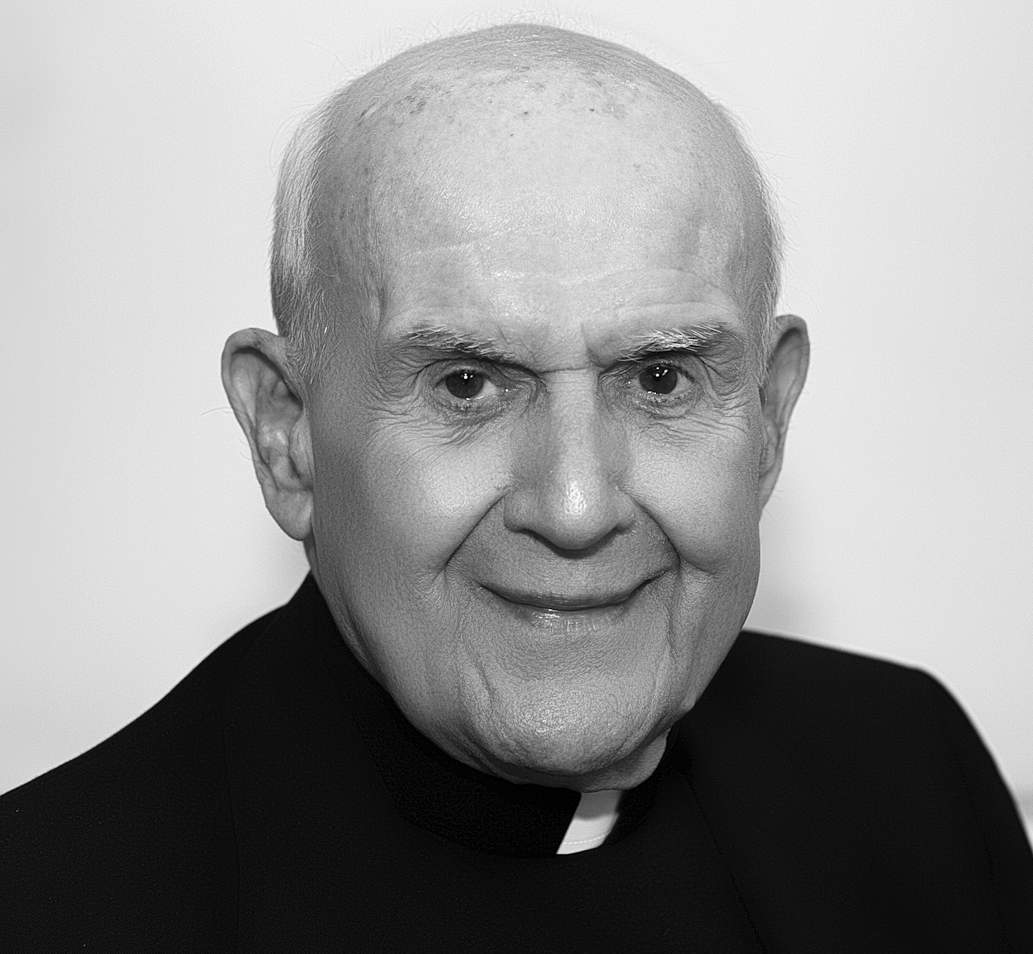
\includegraphics[scale=0.21]{fr-novak}
\lxRDFa{property=novak-graphic,resource={manual}}

\end{center}

% ------------------------------------------------------------------------------

\end{document}
